\documentclass[portuguese, oneside]{pucrs-ppgcc}

\usepackage[square]{natbib}
\usepackage{enumitem}
\usepackage{breakcites}
\usepackage{todonotes,soul}
\usepackage{comment}
\usepackage{cleveref}
\usepackage{booktabs}
\usepackage{xurl}
\usepackage{url}
\usepackage{listings}

\lstset{captionpos=b}
\lstset{basicstyle=\ttfamily\footnotesize}

\newcommand{\cfm}[1]{\todo[size=\tiny,linecolor=blue,backgroundcolor=green!30,bordercolor=black]{FM: #1}}

\newcommand{\cgk}[1]{\todo[size=\tiny,linecolor=blue,backgroundcolor=blue!30,bordercolor=black]{GK: #1}}


\setcounter{secnumdepth}{3}

\hypersetup{
    colorlinks=true,
    linkcolor=blue,
    citecolor=blue,
    filecolor=blue,      
    urlcolor=blue,
}

\setlength {\marginparwidth }{2cm} 


% -------------------------------------------------------------------------------------- %

\author{Gabriel Kaizer de Menezes}

\begin{comment}
    
\title{COMUNICAÇÃO P2P SOBRE QUIC PARA IOT: UMA ABORDAGEM DE BAIXA INFRAESTRUTURA}{P2P COMMUNICATION OVER QUIC FOR IOT: A LOW-INFRASTRUCTURE APPROACH}
\end{comment}

\title{CONECTIVIDADE P2P PARA IOT: ANÁLISE E IMPLEMENTAÇÃO DE HOLE PUNCHING COM O PROTOCOLO QUIC}{}
     
% \tipotrabalho{\ptese} % !!!

\grau{\bacharel}
%\grau{\mestre}
%\grau{\doutor}

\orientador{Fernando Gehm Moraes}

\begin{document}

\begin{agradecimentos}

  Lorem ipsum dolor sit amet, consectetuer adipiscing elit. Aenean commodo ligula eget dolor. Aenean massa. Cum sociis natoque penatibus et magnis dis parturient montes, nascetur ridiculus mus. Donec quam felis, ultricies nec, pellentesque eu, pretium quis, sem. Nulla consequat massa quis enim. Donec pede justo, fringilla vel, aliquet nec, vulputate eget, arcu. In enim justo, rhoncus ut, imperdiet a, venenatis vitae, justo. Nullam dictum felis eu pede mollis pretium. Integer tincidunt. Cras dapibus. Vivamus elementum semper nisi. Aenean vulputate eleifend tellus. Aenean leo ligula, porttitor eu, consequat vitae, eleifend ac, enim. Aliquam lorem ante, dapibus in, viverra quis, feugiat a, tellus. Phasellus viverra nulla ut metus varius laoreet. Quisque rutrum. Aenean imperdiet. Etiam ultricies nisi vel augue. Curabitur ullamcorper ultricies nisi. Nam eget dui. Etiam rhoncus. Maecenas tempus, tellus eget condimentum rhoncus, sem quam semper libero, sit amet adipiscing sem neque sed ipsum. Nam quam nunc, blandit vel, luctus pulvinar, hendrerit id, lorem. Maecenas nec odio et ante tincidunt tempus. Donec vitae sapien ut libero venenatis faucibus. Nullam quis ante. Etiam sit amet orci eget eros faucibus tincidunt. Duis leo. Sed fringilla mauris sit amet nibh. Donec sodales sagittis magna.

%I would like to use this space to express my deepest gratitude towards the people who made this work possible.

%First of all, I thank my advisor, Prof. Fernando Moraes, for the incredible guidance he offered. Thank you for taking me into this project, and for all the help and patience during this last year. I know it wasn't easy at times, and I hugely appreciate the support you've been giving me.

%I also extend my sincere thanks to Prof. Iaçanã Ianiski Weber for the teachings in the course 98G08-04 - Confiabilidade e Segurança de Software. The excellent theoretical foundation built during your classes was absolutely essential for me to fully grasp the highly complex algorithms required for this research.

%I also thank my family, especially my parents, Marildo and Siloé, and my sister, Natália, for the constant support they gave me during my graduation. Without them, none of this would've been possible in the first place.

%Finally, I thank FAPERGS for financing my participation in this research, thus enabling me to pursue this work.

\end{agradecimentos}

\begin{resumo}{Internet das Coisas, gateways, QUIC, travessia de NAT, comunicação P2P}

A comunicação entre aplicações de sistemas de Internet das Coisas (IoT) situadas em redes privadas distintas enfrenta dificuldades de conectividade impostas pela tradução de endereços de rede (NAT). O uso de servidores intermediários para transportar os dados contorna essas dificuldades, mas acrescenta infraestrutura à comunicação. Este trabalho apresenta uma infraestrutura de comunicação ponto a ponto entre \textit{gateways} IoT, utilizando QUIC para transportar dados de aplicações baseadas em TCP e ICE para descobrir e selecionar caminhos de comunicação. A arquitetura do WebRTC serve como referência para a organização das etapas de sinalização e estabelecimento de conectividade. A implementação parte de uma interface modular desenvolvida a partir do Chownat e integra as bibliotecas \texttt{OpenSSL} e \texttt{libnice}, preservando a interface TCP das aplicações. A solução permite utilizar caminhos diretos entre os \textit{gateways} ou retransmissão via TURN, conforme as condições de conectividade. A abordagem busca reduzir a dependência de servidores intermediários para o transporte contínuo dos dados quando um caminho direto estiver disponível, mantendo serviços auxiliares para o estabelecimento das conexões. O escopo concentra-se no transporte entre \textit{hosts} de propósito geral que representam os \textit{gateways}, sem abranger a aquisição de dados por sensores ou a execução das bibliotecas em dispositivos IoT com recursos limitados. A avaliação prevista contempla o funcionamento da integração e o desempenho da comunicação, considerando o tempo de estabelecimento das conexões, o tempo de resposta e a vazão útil.

%O avanço da computação quântica representa uma ameaça direta aos algoritmos criptográficos tradicionais. Para garantir a segurança futura, dispositivos de borda (\textit{edge computing}) e Internet das Coisas (IoT) precisam migrar para padrões de criptografia pós-quântica (PQC), como o algoritmo ML-KEM. No entanto, a alta complexidade computacional desses novos padrões sobrecarrega processadores embarcados limitados por restrições de energia e área. Este trabalho aborda esse desafio propondo a integração de aceleradores escalares dedicados como extensões do conjunto de instruções (ISA) em um processador RISC-V (RS5). O projeto foca na aceleração em hardware das operações mais custosas do ML-KEM: a multiplicação polinomial no domínio da Transformada Numérica de Teoria (NTT) e a compressão de dados. A arquitetura foi avaliada através de prototipagem em FPGA e síntese ASIC utilizando a tecnologia de 28nm da TSMC. A análise da implementação física revelou que abordagens puramente combinacionais para a aritmética pós-quântica degradam o roteamento e violam o fechamento de tempo (\textit{timing closure}). Para solucionar essa limitação, adotou-se uma arquitetura estruturalmente serializada, isolando a lógica criptográfica através de fronteiras de registradores e máquinas de estados. Essa estratégia consolidou um compromisso área-desempenho (\textit{trade-off}) favorável: a integração impôs custos de 5,8\% de aumento na área de silício e 3,4\% na dissipação de potência típica. Em contrapartida, a extensão acelerou a execução e entregou uma redução de 45,1\% na latência de decapsulação do ML-KEM, o que diminuiu o consumo total de energia em 43,3\%. Esse compromisso arquitetural permitiu que o núcleo sustentasse a restrição de 250 MHz sob piores condições operacionais (\textit{worst-case}), validando uma implementação física com eficiência energética otimizada.

\end{resumo}

\begin{abstract}{Internet of Things, gateways, QUIC, NAT traversal, P2P communication}

Communication between Internet of Things (IoT) applications located in different private networks faces connectivity challenges imposed by Network Address Translation (NAT). Using intermediary servers to carry application data overcomes these challenges but adds infrastructure to the communication path. This work presents a peer-to-peer communication infrastructure between IoT gateways, using QUIC to carry data from TCP-based applications and ICE to discover and select communication paths. The WebRTC architecture serves as a reference for organizing signaling and connectivity establishment. The implementation builds on a modular interface developed from Chownat and integrates the \texttt{OpenSSL} and \texttt{libnice} libraries while preserving the applications' TCP interface. The solution supports direct paths between gateways or relaying through TURN, depending on connectivity conditions. The approach aims to reduce reliance on intermediary servers for continuous data transport whenever a direct path is available, while retaining auxiliary services for connection establishment. The scope focuses on transport between general-purpose hosts representing gateways, without covering sensor data acquisition or the execution of these libraries on resource-constrained IoT devices. The planned evaluation addresses integration functionality and communication performance, considering connection establishment time, response time, and application goodput.

% The advancement of quantum computing poses a direct threat to traditional cryptographic algorithms. To ensure future security, edge computing and Internet of Things (IoT) devices must migrate to post-quantum cryptography (PQC) standards, such as the ML-KEM algorithm. However, the computational complexity of these new standards burdens embedded processors constrained by power and area limits. This work addresses this challenge by proposing the integration of dedicated custom scalar accelerators as Instruction Set Architecture (ISA) extensions into an RS5 RISC-V processor. The design focuses on the hardware acceleration of the most computationally expensive ML-KEM operations: Number Theoretic Transform (NTT) polynomial multiplication and data compression. The architecture was evaluated through FPGA prototyping and ASIC synthesis targeting a TSMC 28nm standard-cell library. The physical implementation analysis revealed that purely combinational approaches for post-quantum arithmetic degrade global routing and violate timing closure. To resolve this bottleneck, a structurally serialized architecture was adopted, isolating the cryptographic logic through register boundaries and state machines. This strategy established a clear area-performance trade-off: the integration incurred overheads of a 5.8\% increase in silicon footprint and a 3.4\% rise in typical power dissipation. In return, the custom extension achieved a 45.1\% reduction in ML-KEM decapsulation latency and decreased total energy consumption by 43.3\%. This architectural compromise allowed the core to sustain the 250 MHz constraint under worst-case operating conditions, validating a physical implementation with optimized efficiency.
\end{abstract}

\listoffigures       % Lista de figuras      (OPCIONAL)
\listoftables        % Lista de tabelas      (OPCIONAL)
%\listofalgorithms    % Lista de algoritmos   (OPCIONAL)
\listofacronyms      % Lista de siglas       (OPCIONAL)
%----------------------------------------------------------------------------------
% Lista de siglas. Cada comando alimenta a "List of Acronyms" (\listofacronyms).
% \sigla (definido na classe) converte a sigla para CAIXA ALTA.
% \siglapres preserva a grafia original -- usado em IoT, IPv4, IPv6, VoIP, WebRTC.
% As entradas aparecem na ordem abaixo; mantenha-a alfabetica.
%----------------------------------------------------------------------------------
\providecommand{\siglapres}[2]{\addcontentsline{los}{acronym}{#1\nobreakspace--\nobreakspace #2}}

\sigla{ACK}{Acknowledge}
\sigla{ADF}{Address Dependent Filtering}
\sigla{ADM}{Address Dependent Mapping}
\sigla{AEAD}{Authenticated Encryption with Associated Data}
\sigla{AES}{Advanced Encryption Standard}
\sigla{AES-CM}{Advanced Encryption Standard - Counter Mode}
\sigla{APDF}{Address and Port Dependent Filtering}
\sigla{APDM}{Address and Port Dependent Mapping}
\sigla{API}{Application Programming Interface}
\sigla{CGNAT}{Carrier-Grade NAT}
\sigla{CID}{Connection ID}
\sigla{CSPRNG}{Cryptographically Secure Pseudorandom Number Generator}
\sigla{DCID}{Destination Connection ID}
\sigla{DHE}{Diffie-Hellman Ephemeral}
\sigla{DTLS}{Datagram Transport Layer Security}
\sigla{ECB}{Electronic Code Book}
\sigla{ECDHE}{Elliptic Curve Diffie-Hellman Ephemeral}
\sigla{EDM}{Endpoint Dependent Mapping}
\sigla{EIF}{Endpoint Independent Filtering}
\sigla{EIM}{Endpoint Independent Mapping}
\sigla{GIPS}{Global IP Solutions}
\sigla{GNS3}{Graphical Network Simulator-3}
\sigla{GQUIC}{Google QUIC}
\sigla{HKDF}{HMAC-based Key Derivation Function}
\sigla{HMAC-SHA1}{Hash-based Message Authentication Code - Secure Hash Algorithm 1}
\sigla{HTTP}{Hypertext Transfer Protocol}
\sigla{HTTP/2}{HyperText Transfer Protocol Version 2}
\sigla{HTTP/3}{HyperText Transfer Protocol Version 3}
\sigla{ICE}{Interactive Connectivity Establishment}
\sigla{ICMP}{Internet Control Message Protocol}
\sigla{ID}{Identifier}
\sigla{IETF}{Internet Engineering Task Force}
\siglapres{IoT}{Internet of Things}
\sigla{IP}{Internet Protocol}
\siglapres{IPv4}{Internet Protocol Version 4}
\siglapres{IPv6}{Internet Protocol Version 6}
\sigla{IQUIC}{IETF QUIC}
\sigla{ISP}{Internet Service Provider}
\sigla{IV}{Initialization Vector}
\sigla{LAN}{Local Area Network}
\sigla{NAPT}{Network Address Port Translation}
\sigla{NAT}{Network Address Translator}
\sigla{NAT-PT}{Network Address Translation - Protocol Translation}
\siglapres{Nonce}{Number Used Once}
\siglapres{NPTv6}{IPv6-to-IPv6 Network Prefix Translation}
\sigla{OSI}{Open Systems Interconnection}
\sigla{P2P}{Peer-to-peer}
\sigla{PAT}{Port Address Translation}
\sigla{PSK}{Pre Shared Key}
\sigla{PSTN}{Public Switched Telephone Network}
\sigla{PTO}{Probe Timeout}
\siglapres{QoS}{Quality of Service}
\sigla{RFC}{Request for Comments}
\sigla{RTCP}{RTP Control Protocol}
\sigla{RTO}{Retransmission Timeout}
\sigla{RTP}{Real-time Transport Protocol}
\sigla{RTT}{Round Trip Time}
\sigla{SCID}{Source Connection ID}
\sigla{SCTP}{Stream Control Transmission Protocol}
\sigla{SDP}{Session Description Protocol}
\sigla{SOHO}{Small-Office-Home-Office}
\sigla{SRTCP}{Secure RTP Control Protocol}
\sigla{SRTP}{Secure Real-time Transport Protocol}
\sigla{STUN}{Session Traversal Utilities for NAT}
\sigla{TCP}{Transmission Control Protocol}
\sigla{TLS}{Transport Layer Security}
\siglapres{TLSv1.3}{Transport Layer Security Version 1.3}
\sigla{TURN}{Traversal Using Relays around NAT}
\sigla{UDP}{User Datagram Protocol}
\siglapres{VoIP}{Voice over IP}
\sigla{W3C}{World Wide Web Consortium}
\sigla{WAN}{Wide Area Network}
\siglapres{WebRTC}{Web Real-Time Communication}

%\listofabbreviations % Lista de abreviaturas (OPCIONAL)
%\listofsymbols       % Lista de símbolos     (OPCIONAL)
\tableofcontents     % Sumário               (OBRIGATÓRIO)

\chapter{Introdução}
\label{chap:intro}

A Internet das Coisas (IoT, do inglês \textit{Internet of Things}) tem se destacado como um campo em expansão, impulsionado pelo uso crescente de ferramentas de automação no cotidiano. Essas ferramentas demandam o controle e a gerência ágeis de dados, tarefas frequentemente vinculadas à leitura de sensores e à atuação em tempo real sobre dispositivos de uso diário. Esse cenário abrange diversas áreas, como segurança patrimonial, controle de veículos autônomos e medicina.

Nesse contexto, a comunicação entre os dispositivos deve atender aos requisitos de dependabilidade e segurança descritos em \citep{Avizienis2004}, pois falhas, indisponibilidade ou comprometimento dos dados podem afetar diretamente o funcionamento dos sistemas e, em aplicações críticas, gerar consequências graves. Além disso, o grande volume de dados potencialmente sensíveis transmitidos por esses dispositivos torna essencial a confidencialidade das informações. Nesse sentido, mecanismos criptográficos devem proteger o conteúdo das mensagens e, quando possível, os metadados da comunicação, frequentemente expostos nos cabeçalhos (\textit{headers}) dos protocolos e capazes de revelar informações sobre a conexão. Esses metadados podem revelar padrões de comunicação e outras informações que não deveriam ser acessíveis a terceiros não autorizados.

Este trabalho tem origem em um projeto desenvolvido em conjunto com a DATACOM, cujo objetivo era viabilizar a comunicação entre aplicações situadas em redes distintas, com o mínimo de infraestrutura intermediária. O projeto explorou técnicas de travessia de NAT (\textit{NAT traversal}) e o tunelamento de tráfego TCP sobre UDP, tomando como base o Chownat. A partir desse desenvolvimento, o presente trabalho aprofunda a integração do QUIC com mecanismos de estabelecimento de conectividade baseados em ICE e considera sua aplicação à comunicação entre \textit{gateways} de sistemas IoT.

A solução proposta consiste em uma infraestrutura de comunicação ponto a ponto entre \textit{gateways} de sistemas IoT situados em redes distintas. A proposta integra um modelo de arquitetura baseado no padrão WebRTC (\textit{Web Real-Time Communication}) \citep{WebRTCForTheCurious} que gerencia aplicações baseadas em TCP por meio de conexões locais e utiliza o protocolo de transporte QUIC \citep{rfc9000} para transportar seus dados entre os \textit{gateways}, utilizando o protocolo ICE \citep{rfc8445} para descobrir e selecionar caminhos de comunicação. O escopo experimental concentra-se no transporte entre \textit{hosts} de propósito geral que representam os \textit{gateways}, sem incluir a aquisição de dados por sensores ou a comunicação local com dispositivos IoT. A proposta visa aprimorar o seguinte conjunto de atributos de segurança e dependabilidade na transmissão de dados em aplicações IoT:

\begin{comment}
    
Este trabalho propõe uma infraestrutura de rede para a transmissão de dados com baixa latência em uma arquitetura ponto a ponto (P2P, do inglês \textit{peer-to-peer}), baseada no padrão WebRTC (\textit{Web Real-Time Communication}) \citep{WebRTCForTheCurious} e no protocolo de transporte QUIC\footnote{Embora tenha surgido como acrônimo de \textit{Quick UDP Internet Connections}, o termo QUIC é tratado como nome, e não como sigla, em sua especificação \citep{rfc9000}.} \citep{rfc9000}. A proposta visa aprimorar o seguinte conjunto de atributos de segurança e dependabilidade na transmissão de dados em aplicações IoT:

\end{comment}

\begin{itemize}
    \item \textbf{Confidencialidade:} garantia de que os dados transmitidos sejam acessíveis somente a entidades autorizadas.
    \item \textbf{Confiabilidade:} capacidade de um sistema de fornecer corretamente o serviço esperado, de forma contínua, durante um determinado período.
    \item \textbf{Disponibilidade:} prontidão do sistema para fornecer o serviço corretamente quando solicitado.
    \item \textbf{Integridade:} ausência de alterações indevidas no sistema, incluindo modificações não autorizadas nos dados transmitidos.
\end{itemize}
\cfm{ficou boa a intro}
\section{Motivação}

Em sistemas IoT organizados por meio de \textit{gateways}, esses nós assumem a responsabilidade pela comunicação externa das aplicações associadas aos dispositivos locais. Quando situados em redes privadas distintas, os \textit{gateways} precisam de mecanismos que permitam estabelecer conectividade através de NATs. Nesse cenário, a comunicação ponto a ponto pode reduzir a dependência de servidores intermediários para o transporte contínuo dos dados, mantendo serviços auxiliares para a descoberta e o estabelecimento das conexões.

O WebRTC \citep{WebRTCForTheCurious} é um padrão aberto criado para viabilizar a comunicação em tempo real entre navegadores, com baixa latência e infraestrutura reduzida. O padrão estabelece comunicação direta entre pares (\textit{peers}) situados em sub-redes (\textit{subnets}) distintas por meio de técnicas de travessia de NAT (\textit{NAT traversal}) \citep{rfc5128}, isto é, técnicas que permitem a comunicação através de tradutores de endereços de rede (NAT, do inglês \textit{Network Address Translator}). Protocolos como STUN (\textit{Session Traversal Utilities for NAT}), TURN (\textit{Traversal Using Relays around NAT}) e ICE (\textit{Interactive Connectivity Establishment}) implementam essas técnicas. O WebRTC serve como referência arquitetural para este trabalho, especialmente pela organização dos mecanismos de sinalização e estabelecimento de conectividade. A solução proposta utiliza esses mecanismos em conjunto com QUIC para a comunicação entre gateways.

O QUIC \citep{rfc9000}, por sua vez, é um protocolo de transporte que opera sobre o UDP (\textit{User Datagram Protocol}) e foi desenvolvido para superar limitações da comunicação baseada em TCP (\textit{Transmission Control Protocol}). Sua concepção está associada à redução da latência e à integração de mecanismos de segurança, inicialmente motivadas pelas necessidades das conexões HTTP (\textit{Hypertext Transfer Protocol}) na Web \citep{marx2020quic}. O QUIC implementa sobre UDP mecanismos de entrega confiável e controle de congestionamento, além de integrar mecanismos de proteção criptográfica ao estabelecimento da conexão. Sua implementação no espaço de usuário também facilita a evolução do protocolo sem depender de alterações no núcleo (\textit{kernel}) dos sistemas operacionais. Essas características motivam a investigação do QUIC como transporte externo entre os gateways. A proposta mantém a interface TCP local das aplicações existentes e transporta seus dados pelo caminho estabelecido com ICE, buscando facilitar a integração sem exigir mudanças no protocolo utilizado por essas aplicações.

\section{Objetivos}

Este trabalho tem por objetivo desenvolver e avaliar uma infraestrutura de comunicação ponto a ponto entre \textit{gateways} de sistemas IoT situados em redes distintas, capaz de integrar aplicações legadas baseadas em TCP a um transporte externo sobre QUIC. A organização da solução tem como referência a arquitetura do WebRTC, especialmente quanto às etapas de sinalização e estabelecimento de conectividade, utilizando ICE para descobrir e selecionar caminhos de comunicação entre os \textit{gateways}. A proposta mantém as conexões TCP das aplicações na interface local de \textit{loopback} e transporta seus dados via QUIC até o \textit{gateway} remoto, buscando preservar a interface de comunicação das aplicações e reduzir a necessidade de modificações em sua implementação.

A avaliação concentra-se no funcionamento e no desempenho da infraestrutura entre \textit{hosts} de propósito geral que representam os \textit{gateways}. Os atributos de confidencialidade, integridade, confiabilidade e disponibilidade apresentados anteriormente orientam a discussão dos mecanismos utilizados e das limitações da solução, considerando as configurações e os cenários efetivamente avaliados. Para alcançar o objetivo geral, são definidos os seguintes objetivos específicos:

\begin{comment}
    
\hl{falar de nat/hole punch nos específicos}

\end{comment}

\begin{itemize}

\item Desenvolver uma interface modular de comunicação que permita integrar diferentes protocolos de transporte e mecanismos de estabelecimento de conectividade, tomando como ponto de partida a arquitetura do Chownat.

\item Implementar o transporte de dados das aplicações TCP locais sobre QUIC, utilizando a biblioteca OpenSSL, de modo a preservar a interface de comunicação dessas aplicações nos \textit{gateways}.

\item Integrar o protocolo ICE por meio da biblioteca \texttt{libnice}, permitindo a descoberta e a seleção de caminhos de comunicação entre os \textit{gateways}, incluindo caminhos diretos e caminhos intermediados por servidores TURN.

\item Verificar o funcionamento da infraestrutura em topologias de rede controladas e sob diferentes configurações de NAT, considerando o estabelecimento de conectividade por \textit{UDP hole punching} ou por retransmissão via TURN, a transferência de dados e o encerramento das conexões.

\item Avaliar o desempenho da comunicação entre \textit{hosts} que representam os \textit{gateways}, considerando o tempo de estabelecimento das conexões, o tempo de resposta e a vazão útil nos cenários e perfis de tráfego definidos para os experimentos.

\end{itemize}

O escopo deste trabalho concentra-se na comunicação externa entre gateways de uma arquitetura IoT. Nos experimentos, esses gateways são representados por hosts de propósito geral que executam a infraestrutura proposta e aplicações locais de geração e recepção de mensagens. Não são avaliadas a aquisição de dados por sensores, a comunicação entre dispositivos IoT e gateways, a execução das bibliotecas em microcontroladores ou a eficiência energética desses dispositivos. Quando forem utilizados dados sintéticos, suas características serão explicitadas na metodologia experimental.

\begin{comment}
    
The \textbf{strategic} objective of this undergraduate thesis is to enhance the performance of the Kyber workflow along with its underlying symmetric cryptographic primitives. This involves modifying the RS5 processor to support hardware accelerators for the key generation, encapsulation, and decapsulation phases of the algorithm. The work focuses on optimizing the Number Theoretic Transform (NTT) operation, the primary computational bottleneck, while also integrating standard RISC-V extensions to accelerate the essential SHA-2 and SHA-3 hashing and bit-manipulation tasks. To achieve this general goal, the \textbf{specific} objectives are:

\begin{enumerate}[label=\Roman*]

\item \label{obj_toolchain} {\bf Toolchain Modification}.\\
     Modify and rebuild the compiler toolchain to support the custom XKYBER instructions.

\item \label{obj_zknh} {\bf ZKNH Extension Integration}.\\
     Integrate the ZKNH extension into the RS5 processor to accelerate SHA-2 cryptographic hashing, a feature specifically implemented to fulfill the requirements of the WIMED project.

\item \label{obj_xkyber} {\bf XKYBER Custom Instruction Set}.\\
    Port and integrate the XKYBER custom instruction set to optimize the core operations of the Kyber workflow. The original XKyber extension was developed in \citep{carlos24}. 

\item \label{obj_zbkb} {\bf ZBKB Extension Addition}.\\
     Add the ZBKB extension to accelerate SHA-3 bit-manipulation tasks.

\item \label{obj_verification} {\bf Functional Verification and Evaluation}.\\
     Verify the functional correctness of the integrated modules and evaluate the resulting performance improvements.

\item \label{obj_synthesis} {\bf Post-Synthesis Analysis}.\\
     Perform post-synthesis analysis to assess hardware resource utilization and achieve timing closure.

\end{enumerate}
\end{comment}

\section{Organização do Documento}

Este documento está organizado da seguinte forma:

\begin{itemize}

\item O Capítulo~\ref{chap:background} apresenta os fundamentos de comunicação necessários à compreensão da solução, incluindo os modelos de arquitetura de rede, o papel dos \textit{gateways}, o funcionamento do NAT, as técnicas de travessia de NAT e os protocolos STUN, TURN e ICE. Também são apresentados o Chownat e a relação da proposta com a arquitetura do WebRTC.

\item O Capítulo~\ref{chap:quic} descreve o protocolo QUIC, abordando sua estrutura, os mecanismos de estabelecimento e manutenção das conexões, o transporte de dados e sua utilização em conjunto com técnicas de travessia de NAT.

\item O Capítulo~\ref{chap:implementation} detalha a implementação da infraestrutura proposta, os ambientes e as topologias de teste, o desenvolvimento das interfaces de comunicação, o tunelamento das aplicações TCP locais e a integração das bibliotecas OpenSSL e \texttt{libnice} para a comunicação entre os \textit{gateways}.
    
\item O Capítulo~\ref{chap:results} apresenta a metodologia de avaliação e os resultados dos testes de funcionamento e desempenho, discutindo o comportamento da infraestrutura nos cenários considerados e as limitações da avaliação experimental.

\item O Capítulo~\ref{chap:conclusion} apresenta as conclusões do trabalho, relacionando os resultados aos objetivos estabelecidos e indicando possibilidades de continuidade e trabalhos futuros.


\end{itemize}

\begin{comment}
    
This work is organized as follows:

\begin{itemize}
    \item \Cref{chap:notation} defines the foundational terminology, acronyms, and mathematical notation utilized throughout the text, strictly aligned with the NIST FIPS 203 standard.
    
    \item \Cref{chap:background} provides the theoretical foundation required to comprehend this work, including the fundamentals of the ML-KEM algorithm, polynomial arithmetic over rings, and the NTT operation, which is the most complex part.
    
    \item \Cref{chap:xkyber} details the core contribution of this work: the integration of the custom scalar cryptographic extensions. It covers the structural evolution of the \texttt{kybermul} and \texttt{kybercompress} instructions, from the initial combinational versions to the final serialized implementations.
    
    \item \Cref{chap:results} evaluates the physical hardware implementation, presenting the ASIC synthesis results targeting a 28nm standard-cell library in GENUS and FPGA synthesis in Vivado. This chapter discusses execution latency, area footprints, power dissipation, and the necessary physical trade-offs required to achieve timing closure.
   
    \item \Cref{chap:conclusion} concludes this work, summarizing the findings regarding the physical cost of embedding post-quantum security into embedded processors, and points out directions for future research.
\end{itemize}
\end{comment}








%\chapter{Terms, Acronyms, and Notation}
\label{chap:notation}

Este capítulo estabelece a terminologia, as siglas e a notação matemática utilizadas ao longo deste trabalho. Para garantir a conformidade com a padronização atual dos protocolos de comunicação, as definições e os símbolos apresentados seguem os documentos oficiais de Request for Comments (RFC) da Internet Engineering Task Force (IETF).

\section{Terms and Definitions}

TBD

\begin{comment}
\todo{FAZER ESSA SEÇÃO}

\begin{description}
    \item[Cryptographic module: ] The set of hardware, software, and/or firmware that implements approved cryptographic functions (including key generation) that are contained within the cryptographic boundary of the module.
    \item[Decapsulation: ] The process of applying the Decaps algorithm of a KEM. This algorithm accepts a KEM ciphertext and the decapsulation key as input and produces a shared secret key as output.
    \item[Encapsulation: ] The process of applying the Encaps algorithm of a KEM. This algorithm accepts the encapsulation key as input, requires private randomness, and produces a shared secret key and an associated ciphertext as output.
    \item[(KEM) Ciphertext: ] A bit string that is produced by encapsulation and used as an input to decapsulation.
    \item[Shared secret key: ] A shared secret that can be used directly as a cryptographic key in symmetric-key cryptography. It does not require additional key derivation.
    \item[Security strength: ] A number associated with the amount of work (i.e., the number of operations) that is required to break a cryptographic algorithm or system.
\end{description}
\end{comment}


% \section{Mathematical Symbols}

\begin{comment}
    
The implementation of ML-KEM relies on polynomial arithmetic over rings. The mathematical notation utilized for the algorithmic description and hardware acceleration is defined below.

\begin{table}[!ht]
\renewcommand{\arraystretch}{1.5}
\centering
\begin{tabular}{@{}lp{13cm}@{}}
\toprule
\textbf{Symbol} & \textbf{Description} \\ \midrule
$n$ & Denotes the integer 256 throughout this document. \\
$q$ & Denotes the prime integer $3329 = 2^8 \cdot 13 + 1$ throughout this document. \\
$\zeta$ & Denotes the integer 17, which is a primitive $n$-th root of unity modulo $q$. \\
$\mathbb{B}$ & The set $\{0, 1, \dots, 255\}$ of unsigned 8-bit integers (bytes). \\
$\mathbb{Z}_q$ & The ring of integers modulo $q$ (i.e., the set $\{0, 1, \dots, q-1\}$ equipped with the operations of addition and multiplication modulo $q$). \\
$R_q$ & The ring $\mathbb{Z}_q[X]/(X^n + 1)$ consisting of polynomials of the form $f = f_0 + f_1X + \dots + f_{255}X^{255}$, where $f_j \in \mathbb{Z}_q$ for all $j$. \\
$T_q$ & The image of $R_q$ under the number-theoretic transform. Its elements are called ``NTT representations'' of polynomials in $R_q$. \\
$\hat{f}$ & The element of $T_q$ that is equal to the NTT representation of a polynomial $f \in R_q$. \\
$f_j$ & The coefficient of $X^j$ of a polynomial $f \in R_q$. \\
$\mathcal{D}_\eta(R_q)$ & A certain distribution of polynomials in $R_q$ with small coefficients, from which noise is sampled. \\
$\times_{T_q}$ & Denotes the operation on coefficient arrays that implements product in the ring $T_q$. \\
$\lceil x \rceil$ & The ceiling of $x$ (i.e., the smallest integer greater than or equal to $x$). \\
$\lfloor x \rfloor$ & The floor of $x$ (i.e., the largest integer less than or equal to $x$). \\
$\lfloor x \rceil$ & The rounding of $x$ to the nearest integer. \\
$A \parallel B$ & The concatenation of two arrays or bit strings $A$ and $B$. \\
$\text{BitRev}_7(r)$ & Bit reversal of a seven-bit integer $r$. \\
\bottomrule
\end{tabular}
\end{table}
\end{comment}
\include{src/2_relatedWorks}
\chapter{Protocolos de comunicação}
\label{chap:background}

Este capítulo apresenta os conceitos e os protocolos de comunicação que fundamentam a solução proposta neste trabalho, a qual implementa o QUIC sobre uma infraestrutura baseada em WebRTC. O capítulo está organizado da seguinte forma: \cfm{tive que organizar uma introdução}

\begin{itemize}

\item A Seção \ref{sec:protocol_stack} situa os protocolos abordados nos modelos de referência OSI (\textit{Open Systems Interconnection}) e TCP/IP (\textit{Transmission Control Protocol/Internet Protocol}) e delimita as camadas de rede e de transporte como foco do trabalho.

\item A Seção \ref{sec:network_architecture_models} apresenta os modelos arquiteturais de rede --- cliente-servidor, \textit{peer-to-peer} e híbrido --- e sua relação com a solução proposta.

\item A Seção \ref{sec:network_address_translator} descreve o funcionamento do NAT, suas características e classificações, bem como o problema que ele impõe à comunicação P2P.

\item A Seção \ref{sec:nat_traversal} expõe as técnicas de travessia de NAT, incluindo \textit{relaying}, \textit{connection reversal} e \textit{hole punching} sobre UDP e TCP.

\item A Seção \ref{sec:ice} apresenta o protocolo ICE e os servidores STUN e TURN empregados na descoberta e seleção de candidatos de comunicação.

\item A Seção \ref{sec:chownat} detalha a arquitetura e o protocolo Chownat, incluindo os tipos de pacotes e as etapas de conexão e comunicação.
\item A Seção \ref{sec:webrtc} descreve a arquitetura e o protocolo WebRTC, abrangendo sinalização, estabelecimento de conexão, segurança e a API (\textit{Application Programming Interface}).

% \item A Seção \ref{sec:quic} apresenta o protocolo QUIC, sua motivação em relação ao TCP e seu uso em aplicações P2P, incluindo cenários de tempo real e IoT.

\end{itemize}

O protocolo QUIC também integra a pilha de protocolos de comunicação; entretanto, devido à sua complexidade e relevância para este trabalho, o Capítulo~\ref{chap:quic} o aborda separadamente.

%%%%%%%%%%%%%%%%%%%%%%%%%%%%%%%%%%%%%%%%%%%%%%%%%%%%%%%%%%%%%%%%%%%%%%%%%%%%%%%%%%%
% OSI AND TCP/IP STACK
%%%%%%%%%%%%%%%%%%%%%%%%%%%%%%%%%%%%%%%%%%%%%%%%%%%%%%%%%%%%%%%%%%%%%%%%%%%%%%%%%%%
\section{Relações da Pilha de Protocolos}
\label{sec:protocol_stack}

Para compreender a relação entre os protocolos abordados neste trabalho, é necessário entender como eles se organizam nas pilhas de rede. O modelo OSI \citep{iso7498} define uma referência de sete camadas, que serve como abstração para a organização das funções de comunicação em redes. Posteriormente, consolidou-se a arquitetura de protocolos da Internet, comumente denominada arquitetura TCP/IP, que organiza as funções de comunicação em quatro camadas \citep{rfc1122}. Modelos de cinco camadas também representam essa arquitetura, principalmente para distinguir as funções das camadas de enlace e física. Este trabalho adota o modelo de cinco camadas como referência. A Figura~\ref{fig:osi_tcpip} apresenta essas camadas e suas correspondências com o modelo OSI.

\begin{figure}[!ht]
        \centering
        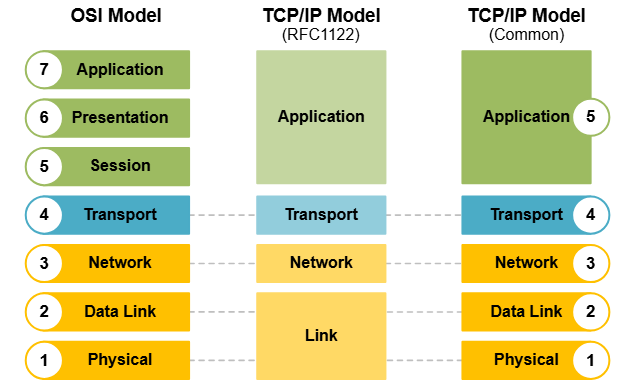
\includegraphics[width=0.7\linewidth]{fig/relationship/osi_tcpip.png}
        \caption{Comparação entre os modelos OSI e TCP/IP por \citep{networkacademy2026osi}.}
        \label{fig:osi_tcpip}
\end{figure}

Este trabalho concentra-se nas camadas de rede e de transporte, correspondentes às camadas 3 e 4 do modelo OSI. A camada de rede é responsável pelo endereçamento e pelo encaminhamento de pacotes entre diferentes redes, enquanto a camada de transporte é responsável pela comunicação fim a fim entre os \textit{peers}. Na arquitetura TCP/IP, essas funções correspondem, respectivamente, às camadas de Internet (\textit{Internet layer}) e de transporte (\textit{transport layer}) \citep{rfc1122}.

Este trabalho utiliza uma infraestrutura baseada em WebRTC, descrita na Seção~\ref{sec:webrtc}. Nessa infraestrutura, a comunicação entre os \textit{peers} depende dos mecanismos de travessia de NAT, descritos na Seção~\ref{sec:nat_traversal}, e do protocolo ICE, apresentado na Seção~\ref{sec:ice}, que realiza a descoberta e a seleção de candidatos de conexão. Sobre essa infraestrutura, o QUIC, descrito no Capítulo~\ref{chap:quic}, atua como protocolo de transporte e encapsula a comunicação TCP entre os \textit{peers}.

A arquitetura considerada neste trabalho é composta por dois \textit{peers} e por servidores auxiliares empregados pelos mecanismos de travessia de NAT. Cada \textit{peer} é um \textit{gateway} associado a um dispositivo IoT ou a uma aplicação consumidora dos dados gerados por esse dispositivo, representados na figura como \textit{device1} e \textit{device2}. Essa aplicação pode ser executada em um sistema de propósito geral ou em outro dispositivo IoT. Os \textit{gateways} executam a infraestrutura proposta e são distintos dos roteadores de acesso, responsáveis pelo encaminhamento dos pacotes e pela tradução de endereços nas redes representadas. As aplicações locais assumem os papéis de cliente e servidor, enquanto os \textit{gateways} viabilizam a comunicação entre elas.

A Figura~\ref{fig:quic_p2p_architecture} apresenta a arquitetura de comunicação proposta neste trabalho, com seus principais elementos e as relações entre eles. Este capítulo descreve os fundamentos teóricos das operações realizadas entre os \textit{peers}, os servidores e os demais elementos da arquitetura, e o Capítulo~\ref{chap:implementation} apresenta a implementação prática dessas operações.

\begin{figure}[!ht]
        \centering
        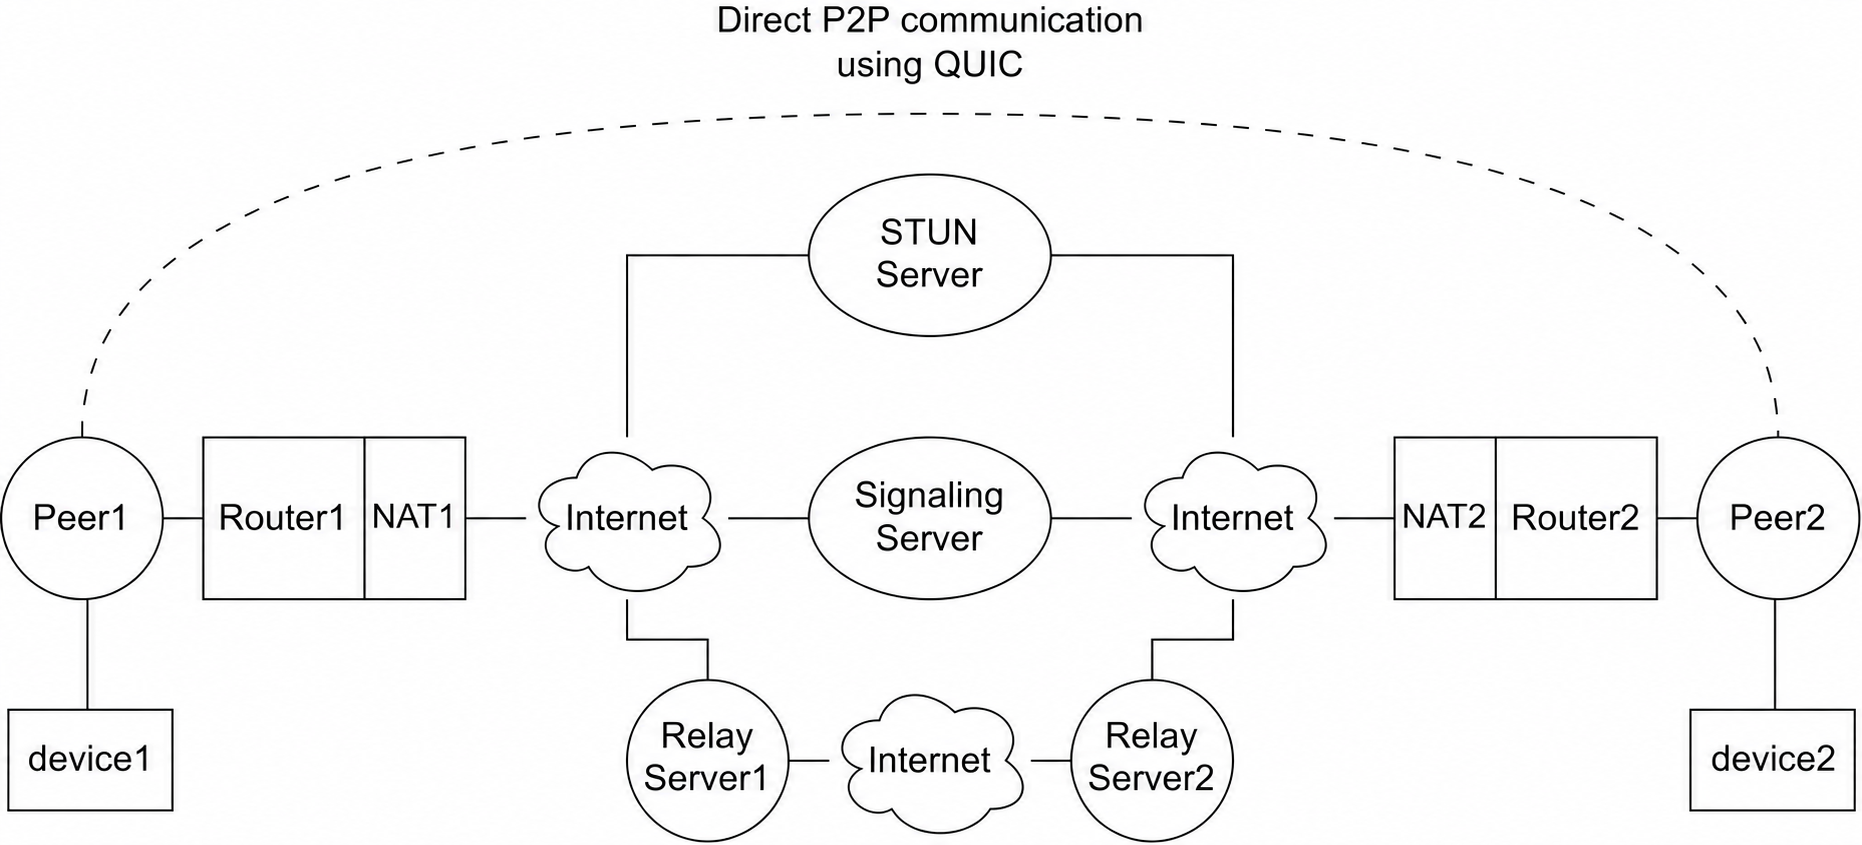
\includegraphics[width=1.0\linewidth]{fig/relationship/architecture_for_quic_p2p.png}
        \caption{Arquitetura para comunicação P2P com QUIC.}
        \label{fig:quic_p2p_architecture}
\end{figure}


%%%%%%%%%%%%%%%%%%%%%%%%%%%%%%%%%%%%%%%%%%%%%%%%%%%%%%%%%%%%%%%%%%%%%%%%%%%%%%%%%%%
% P2P NETWORKS
%%%%%%%%%%%%%%%%%%%%%%%%%%%%%%%%%%%%%%%%%%%%%%%%%%%%%%%%%%%%%%%%%%%%%%%%%%%%%%%%%%%
\section{Modelos de Arquitetura de Rede}
\label{sec:network_architecture_models}

O modelo de arquitetura de rede define a forma como os participantes de uma comunicação interagem entre si e os papéis que desempenham durante a prestação de um serviço. Esse modelo é frequentemente confundido com a topologia da rede, mas os conceitos são distintos: a arquitetura descreve o comportamento e as responsabilidades dos participantes, enquanto a topologia define como os dispositivos estão interconectados, seja física ou logicamente. Dessa forma, uma mesma arquitetura pode operar sobre diferentes topologias, conforme a aplicação. Entre os modelos arquiteturais mais utilizados, destacam-se as arquiteturas cliente-servidor e P2P.

Na prática, não existe uma fronteira rígida entre os diferentes modelos arquiteturais. Conforme discutido em \citep{RFC5694}, arquiteturas P2P e arquiteturas centralizadas não constituem categorias completamente disjuntas, e soluções híbridas são comuns. Nesses casos, diferentes modelos arquiteturais coexistem em uma mesma aplicação e assumem maior ou menor relevância conforme a etapa da comunicação. As aplicações WebRTC (Seção~\ref{sec:webrtc}) exemplificam esse comportamento: a sinalização e a identificação de candidatos pelo protocolo ICE seguem, em geral, o modelo cliente-servidor, por meio de um servidor de sinalização e dos servidores STUN e TURN, enquanto a troca de dados ocorre, sempre que possível, diretamente entre os pares, o que caracteriza uma comunicação P2P.

\subsection{Modelo Cliente-Servidor}

O modelo cliente-servidor é um dos mais utilizados em sistemas distribuídos. Nele, as entidades participantes assumem papéis distintos: o servidor disponibiliza serviços ou recursos, enquanto o cliente oferece uma interface para requisitar e utilizar esses serviços. Em razão dessa divisão de responsabilidades, esse modelo recebe também a denominação de modelo de acesso remoto (\textit{remote access model}) \citep{Tanenbaum2007}, no qual o cliente solicita a execução de operações e o servidor as executa e retorna os resultados. A Figura~\ref{fig:tannenbaum_client_server} ilustra esse modelo.

\begin{figure}[!ht]
        \centering
        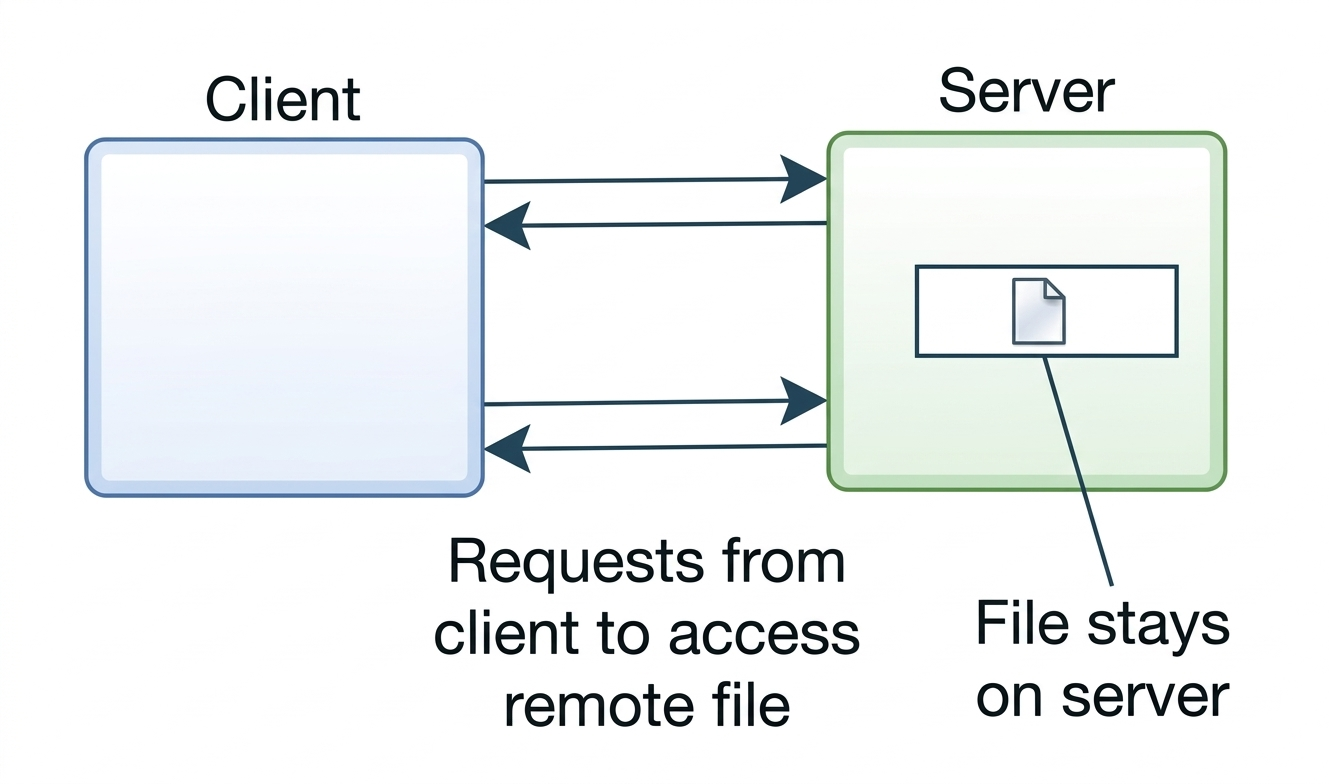
\includegraphics[width=0.5\linewidth]{fig/NetworkModels/client_server.jpg}
        \caption{Diagrama de alto nível do modelo de acesso remoto cliente-servidor, baseado em \citep{Tanenbaum2007}.}
        \label{fig:tannenbaum_client_server}
\end{figure}

\subsection{Modelo Peer-to-Peer}
\label{sec:p2p_model}

A arquitetura P2P caracteriza-se pela distribuição das responsabilidades entre os participantes da rede, sem papéis fixos de cliente e servidor. Dessa forma, um mesmo nó pode atuar tanto como provedor quanto como consumidor de serviços ao longo da comunicação. Apesar do uso amplo dessa arquitetura, não existe uma definição única para sistemas P2P, e a literatura apresenta diferentes interpretações, que variam conforme as características consideradas essenciais para esse modelo. Além disso, durante muitos anos, a arquitetura P2P foi associada ao compartilhamento de conteúdo ilegal. Essa associação, entretanto, decorre das aplicações desenvolvidas sobre essa arquitetura, e não do modelo arquitetural em si.

De acordo com a definição proposta no RFC (\textit{Request for Comments}) 5694 \citep{RFC5694}, um sistema P2P caracteriza-se pelo compartilhamento de recursos entre seus participantes para prover o serviço para o qual foi projetado. Nessa definição, os pares devem tanto fornecer serviços a outros participantes quanto requisitar serviços deles, e contribuem coletivamente para o funcionamento do sistema.

Diversos autores, como \citep{Milojicic2002}, apresentam o modelo cliente-servidor como uma arquitetura centralizada e o modelo P2P como uma arquitetura descentralizada. Essa distinção, entretanto, não constitui uma separação absoluta: conforme discutido na Seção~\ref{sec:network_architecture_models}, sistemas classificados como P2P podem conter componentes centralizados \citep{RFC5694}. A Figura~\ref{fig:centralized_vs_p2p} ilustra a comparação entre os dois modelos.


\begin{figure}[!ht]
        \centering
        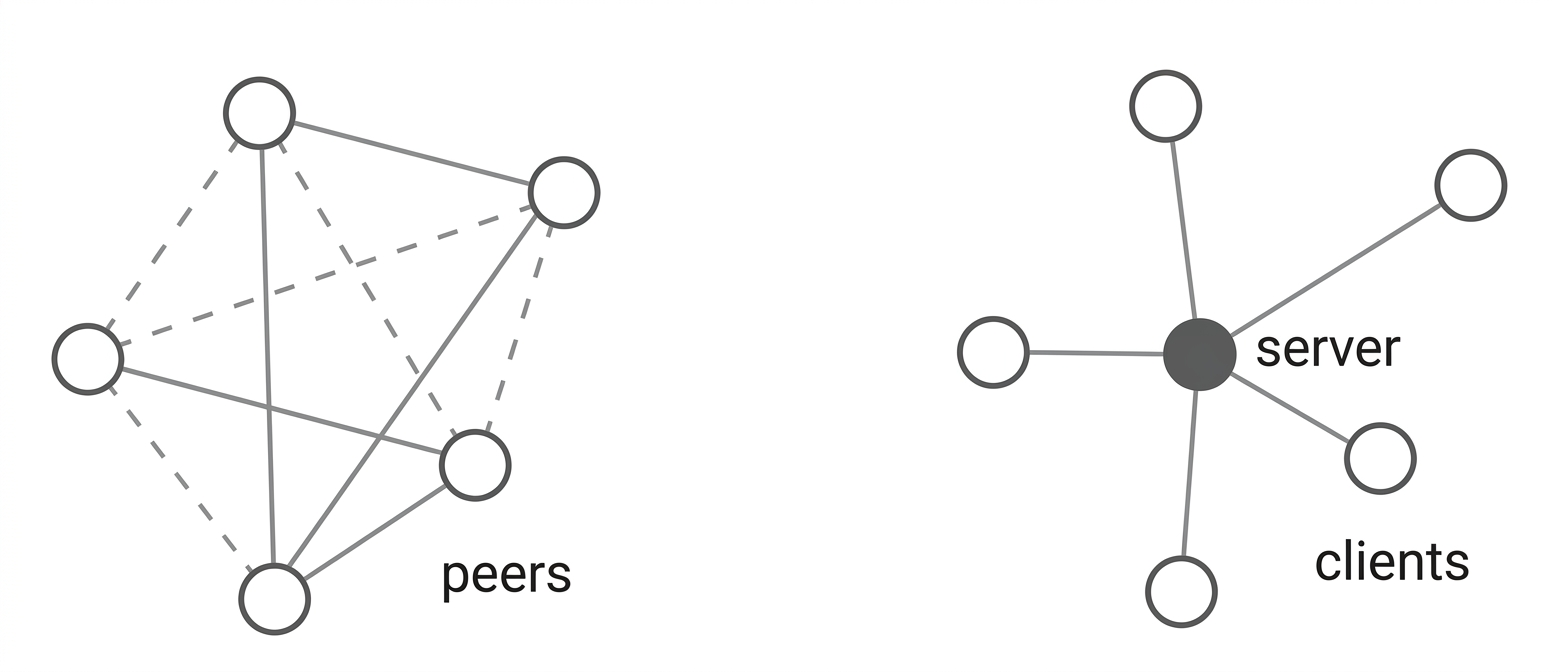
\includegraphics[width=0.6\linewidth]{fig/NetworkModels/centralized_vs_p2p.jpg}
        \caption{Diagrama de alto nível da comparação entre os modelos P2P e centralizado, baseado em \citep{Milojicic2002}.}
        \label{fig:centralized_vs_p2p}
\end{figure}

\subsection{Modelo Peer-to-Peer Híbrido}
\label{sec:hybrid_peer_to_peer_model}

Modelos P2P híbridos combinam características das arquiteturas cliente-servidor e P2P e, portanto, não pertencem exclusivamente a nenhuma delas. Nesses modelos, a comunicação principal ocorre entre os pares, porém determinadas funcionalidades, como autenticação, descoberta de pares, sinalização ou obtenção de metadados necessários à conexão, dependem de um servidor central \citep{Milojicic2002}.

A Figura~\ref{fig:hybrid_p2p} apresenta um exemplo desse modelo. Na Figura~\ref{fig:hybrid_p2p}(a), um \textit{peer} arbitrário A comunica-se com um servidor para obter as informações necessárias à conexão. Em seguida, conforme a Figura~\ref{fig:hybrid_p2p}(b), o \textit{peer} A utiliza essas informações para estabelecer uma comunicação direta com um \textit{peer} arbitrário B.

\begin{figure}[!ht]
        \centering
        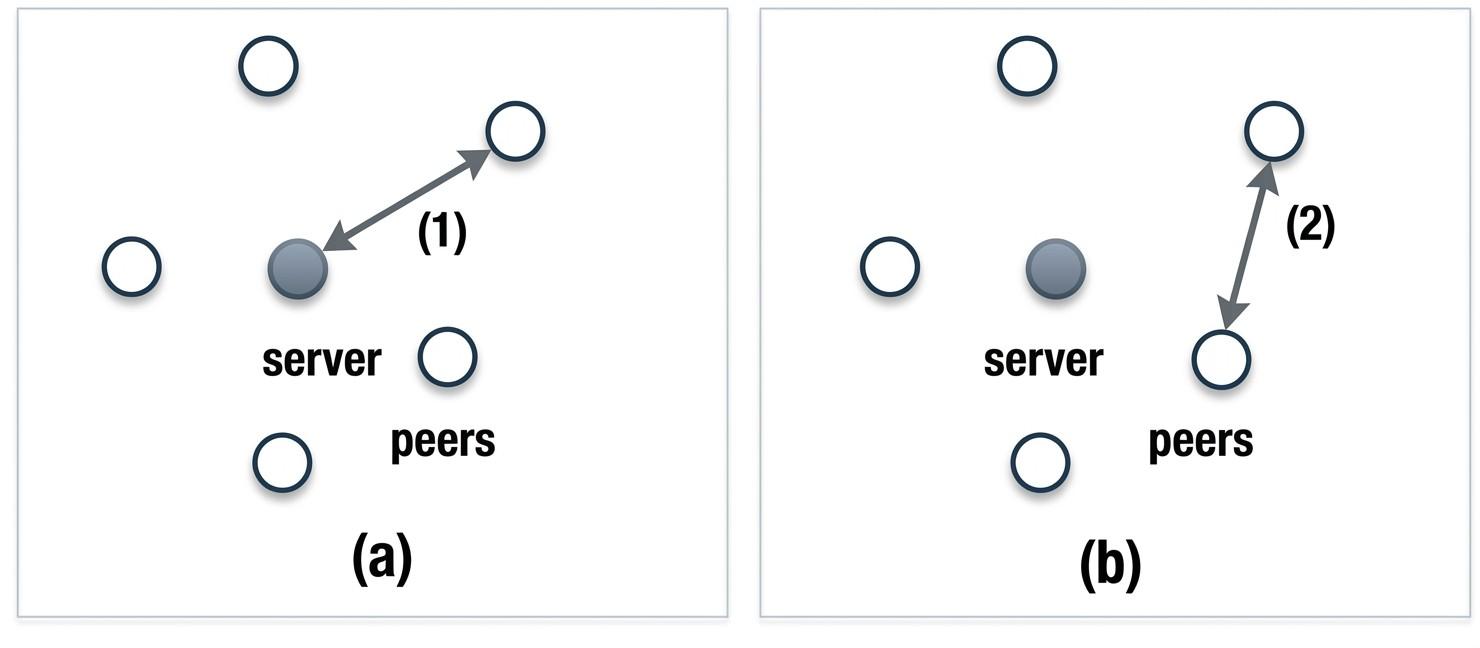
\includegraphics[width=0.6\linewidth]{fig/NetworkModels/hybrid_model.jpg}
        \caption{Exemplo de modelo híbrido, baseado em \citep{Milojicic2002}.}
        \label{fig:hybrid_p2p}
\end{figure}

\subsection{WebRTC como referência arquitetural}
\label{sec:webrtc}

O WebRTC (\textit{Web Real-Time Communication}) permite a comunicação de áudio, vídeo e dados entre \textit{peers}, tendo sido desenvolvido inicialmente para aplicações de comunicação em tempo real entre navegadores \citep{RFC8825}. Sua organização constitui um exemplo do modelo de arquitetura híbrida apresentado na Seção~\ref{sec:hybrid_peer_to_peer_model}: serviços auxiliares participam do estabelecimento da conexão, enquanto os dados podem ser transportados diretamente entre os participantes. Quando a comunicação direta não é possível, o transporte pode utilizar servidores de retransmissão (\textit{relay}).

A Figura~\ref{fig:webrtc_architecture} apresenta uma visão geral dessa arquitetura, destacando os participantes e os serviços envolvidos no estabelecimento da comunicação.

\begin{figure}[!ht]
        \centering
        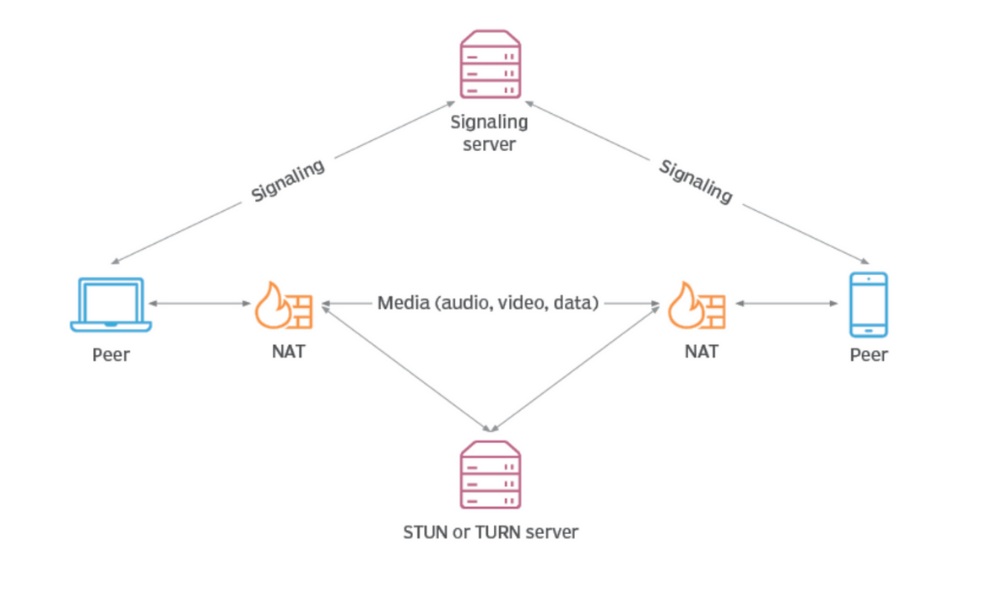
\includegraphics[width=1.0\linewidth]{fig/WebRTC/webrtc_architecture.png}
        \caption{Visão geral da arquitetura do WebRTC, conforme \citep{nugroho2026webrtcwebsocket}.}
        \label{fig:webrtc_architecture}
\end{figure}

DuBois e Ivov \citep{WebRTCForTheCurious} organizam o funcionamento do WebRTC em quatro etapas conceituais:

\begin{itemize}
    \item \textbf{Sinalização (\textit{signaling}):} troca das informações necessárias para que os participantes possam estabelecer a conexão e negociar as características da comunicação. O WebRTC não determina o mecanismo de transporte das mensagens de sinalização, cuja escolha cabe à aplicação.

    \item \textbf{Conexão (\textit{connecting}):} descoberta dos caminhos disponíveis entre os participantes e verificação de sua conectividade. Essa etapa permite selecionar um caminho direto ou retransmitido, conforme as condições das redes envolvidas.

    \item \textbf{Segurança (\textit{securing}):} estabelecimento dos mecanismos de autenticação e proteção criptográfica utilizados na comunicação entre os participantes.

    \item \textbf{Comunicação (\textit{communicating}):} transmissão dos dados das aplicações pelo caminho estabelecido, utilizando os mecanismos de proteção negociados.
\end{itemize}

Essa divisão permite distinguir as responsabilidades envolvidas na comunicação, sem exigir que cada etapa corresponda a um componente isolado. A sinalização viabiliza a troca inicial de informações, a conexão determina o caminho disponível e os mecanismos de segurança e transporte permitem a comunicação protegida entre os participantes.

Neste trabalho, o WebRTC serve como referência arquitetural para a organização dessas responsabilidades, especialmente nas etapas de sinalização e estabelecimento de conectividade entre os \textit{gateways}. A solução utiliza ICE, descrito na Seção~\ref{sec:ice}, para descobrir e selecionar os caminhos de comunicação, e QUIC, apresentado no Capítulo~\ref{chap:quic}, para transportar os dados das aplicações TCP locais e integrar os mecanismos de segurança ao estabelecimento da conexão. A proposta não utiliza a pilha completa ou a API de navegador do WebRTC.

%%%%%%%%%%%%%%%%%%%%%%%%%%%%%%%%%%%%%%%%%%%%%%%%%%%%%%%%
%%%%%%%%%%%%%%%%%%%%%%%%%%%%%%%%%%%%%%%%%%%%%%%%%%%%%%%%
%%%%%%%%%%%%%%%%%%%%%%%%%%%%%%%%%%%%%%%%%%%%%%%%%%%%%%%%
\section{Network Address Translator (NAT)}
\label{sec:network_address_translator}

O NAT é um mecanismo que traduz endereços IP entre diferentes domínios de endereçamento, como uma rede local (LAN, do inglês \textit{Local Area Network}) e uma rede de longa distância (WAN, do inglês \textit{Wide Area Network}). Essa tradução permite que a comunicação entre \textit{hosts} ocorra de forma transparente, sem que os dispositivos finais precisem conhecer ou gerenciar as alterações realizadas pelo dispositivo NAT. Conforme descrito em \citep{RFC1631}, o NAT surgiu principalmente como solução para dois problemas associados ao crescimento da Internet baseada no protocolo IPv4 (\textit{Internet Protocol version 4}): o esgotamento de endereços e a escalabilidade do sistema de roteamento.

\begin{itemize}
\item \textbf{Esgotamento de endereços:} O protocolo IPv4 utiliza endereços de 32 bits, o que permite aproximadamente 4,3 bilhões de endereços distintos. Entretanto, com a expansão da Internet e o aumento do número de dispositivos conectados, esse espaço de endereçamento mostrou-se insuficiente para atender à demanda global.

\item \textbf{Escalabilidade de roteamento:} O crescimento da Internet também aumentou a quantidade de redes e prefixos que precisam ser anunciados e armazenados pelos roteadores da infraestrutura global. A fragmentação do espaço de endereçamento aumenta o tamanho das tabelas de roteamento, o que eleva os requisitos de memória, processamento e atualização dos roteadores responsáveis pelo encaminhamento de pacotes.

\end{itemize}

\subsection{Características em Comum de NATs}

Os diferentes tipos de NAT variam quanto ao modo de realizar as traduções. Entretanto, conforme definido em \citep{RFC2663}, um mecanismo NAT deve apresentar algumas características fundamentais, implementadas de forma completa ou parcial:

\begin{itemize}
\item \textbf{Tradução transparente de endereços:} Os \textit{hosts} envolvidos na comunicação não devem precisar conhecer a existência do NAT nem as traduções realizadas, e devem operar como se a tradução não existisse.

\item \textbf{Encaminhamento transparente através da tradução:} O dispositivo NAT deve encaminhar os pacotes após a tradução de endereços de forma que, para os \textit{hosts} envolvidos, a comunicação ocorra da mesma maneira que ocorreria sem o NAT.

\item \textbf{Tradução do conteúdo de mensagens de erro ICMP:} As mensagens de erro do ICMP (\textit{Internet Control Message Protocol}) carregam em seu conteúdo uma cópia do pacote IP que originou o erro. Como essa cópia pode conter endereços ou informações de transporte modificados pelo NAT, o dispositivo deve traduzir esses campos para que o \textit{host} interno associe corretamente a mensagem de erro à conexão original.

\end{itemize}

Cabe destacar que, no RFC 1631 \citep{RFC1631}, o NAT traduz apenas endereços, enquanto definições posteriores, como a do RFC 3022 \citep{RFC3022}, introduzem o conceito de NAPT (\textit{Network Address Port Translation}), que também traduz portas.

A redução do uso de endereços IP baseia-se no pressuposto de que nem todos os dispositivos de uma rede privada precisam de um endereço IP público. Por isso, o RFC 1631 discute a necessidade de particionar o espaço de endereçamento entre endereços reutilizáveis (locais) e endereços globalmente únicos, sem, no entanto, definir faixas concretas para essa alocação. Em vez disso, o documento remete à alocação proposta no RFC 1597 \citep{rfc1597}. Posteriormente, o RFC 1918 \citep{rfc1918} tornou obsoleto o RFC 1597, manteve as mesmas faixas reservadas e as formalizou como \textit{Best Current Practice}. A Figura~\ref{fig:priv_pub_net_p2pnat} ilustra a relação entre endereços IP públicos e privados.

\begin{figure}[!ht]
        \centering
        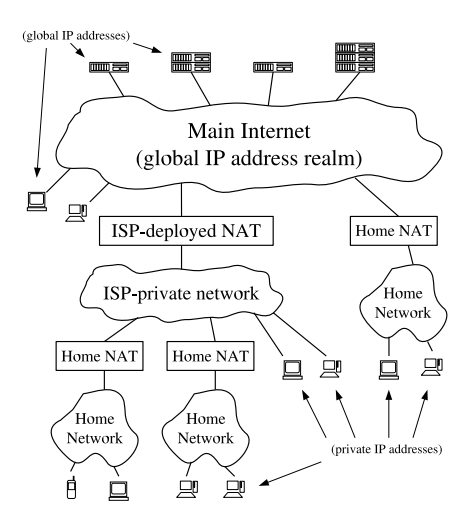
\includegraphics[width=0.5\linewidth]{fig/NATs/priv_pub_net_p2pnat.png}
        \caption{Domínios de endereços IP público e privado por \citep{ford2005peer}.}
        \label{fig:priv_pub_net_p2pnat}
\end{figure}

Entretanto, a reutilização das mesmas faixas de endereços privados em diferentes redes gera sobreposição de endereços: um mesmo endereço privado pode identificar dispositivos distintos em redes diferentes. Essa sobreposição impede que dois dispositivos situados em redes privadas distintas se comuniquem diretamente por meio de seus endereços privados \citep{RFC1631}. Esse problema é central para este trabalho, e a Seção~\ref{sec:nat_problem_for_p2p_communication} o aborda em detalhe.

\subsection{Tipos de NAT}

A literatura classifica os NATs segundo critérios distintos. Para fins de clareza, este trabalho organiza essas classificações em dois eixos: o primeiro relaciona-se ao que é traduzido, e o segundo, ao comportamento da operação de tradução. O primeiro eixo corresponde à nomenclatura do RFC 3022 \citep{RFC3022}, que divide o NAT tradicional (\textit{Traditional NAT}) em NAT básico (\textit{Basic NAT}) e NAPT, este também denominado NAT \textit{overload} ou PAT (\textit{Port Address Translation}). O segundo eixo corresponde à classificação em quatro tipos (\textit{Full Cone}, \textit{Restricted Cone}, \textit{Port-Restricted Cone} e \textit{Symmetric}), definida originalmente no RFC 3489 \citep{RFC3489}. Posteriormente, o RFC 5389 \citep{RFC5389} tornou obsoleto o RFC 3489 e abandonou essa classificação, pois muitos NATs reais não se enquadram de forma precisa em nenhum dos quatro tipos. Em seu lugar, os RFCs 4787 \citep{RFC4787} e 5780 \citep{RFC5780} adotam uma terminologia comportamental mais precisa.

\subsubsection{Classificação de NATs por Tipo de Tradução}
\label{sec:nat_classification_by_translation_type}

O RFC 3022 \citep{RFC3022} amplia o conceito original de tradução do RFC 1631. Enquanto o RFC 1631 prevê a tradução apenas do endereço IP, com mapeamento unívoco (1:1) entre um endereço local e um endereço global, o RFC 3022 formaliza o NAPT, no qual o NAT traduz múltiplos endereços locais, combinados com suas respectivas portas TCP/UDP, para um único endereço público e os diferencia pela porta atribuída. Essa abordagem decorre da necessidade de economizar endereços IPv4 públicos, cada vez mais escassos, e permite que múltiplos dispositivos de uma rede privada compartilhem simultaneamente um único endereço público.

Assim, o RFC 3022 define os seguintes tipos de tradução:
\begin{itemize}
    \item \textbf{\textit{Basic NAT}:} Tradução de endereço (mapeamento 1:1).
    \item \textbf{NAPT:} Tradução de endereço e porta (mapeamento N:1).
\end{itemize}

Além da diferenciação entre \textit{Basic NAT} e NAPT, o RFC 3022 define, de forma ortogonal a essa classificação, o modo de estabelecimento do mapeamento de tradução. No mapeamento estático, a associação entre uma identidade interna e uma identidade global é definida previamente e permanece fixa, o que permite que determinado \textit{host} ou serviço interno utilize sempre o mesmo endereço e a mesma porta globais.

No mapeamento dinâmico, por outro lado, o NAT cria os mapeamentos sob demanda, à medida que os \textit{hosts} da rede privada iniciam comunicações externas. No \textit{Basic NAT}, esse processo implica a alocação temporária de endereços globais aos endereços locais, enquanto no NAPT o dispositivo associa pares de endereço e porta internos a um par de endereço e porta externo disponível.

Dessa forma, o RFC 3022 estabelece dois modos de vinculação (\textit{binding}) aplicáveis tanto ao \textit{Basic NAT} quanto ao NAPT:
\begin{itemize}
    \item \textbf{\textit{Static NAT}:} Associação fixa e predefinida entre uma identidade privada e uma identidade global.
    \item \textbf{\textit{Dynamic NAT}:} Associação entre uma identidade privada e uma identidade global, estabelecida sob demanda a partir de um conjunto disponível.
\end{itemize}

Algumas fontes não normativas tratam o \textit{static} NAT e o \textit{dynamic} NAT como características exclusivas do \textit{Basic NAT}; entretanto, o RFC 3022 não estabelece essa restrição.

\subsubsection{Classificação de NATs por Comportamento de Tradução}
\label{sec:nat_classification_by_translation_behavior}

Os documentos de referência descrevem a classificação comportamental de NATs com diferentes níveis de granularidade. Esta seção apresenta, primeiro, a classificação clássica do RFC 3489, amplamente utilizada na literatura sobre \textit{hole punching} e comunicação P2P, e, em seguida, a classificação comportamental mais recente e detalhada do RFC 4787.

\paragraph{Classificação Clássica}

Além de definir o protocolo STUN e mecanismos de travessia de NAT, abordados nas Seções~\ref{sec:nat_traversal} e~\ref{sec:ice}, o RFC 3489 descreve uma classificação inicial dos tipos de NAT. Embora essa nomenclatura tenha se tornado obsoleta, ela permanece amplamente utilizada por motivos didáticos, e este trabalho a adota. Ainda assim, para manter a coerência com a terminologia atual, este trabalho apresenta, na sequência, as definições mais recentes.

O RFC 3489 trata apenas do NAPT, e não do \textit{Basic NAT}. Entretanto, é possível inferir que os tipos de NAT descritos a seguir se aplicam de forma semelhante ao \textit{Basic NAT}, com exceção do \textit{Symmetric} NAT, que exigiria um endereço externo distinto para cada destino. Como o NAPT estende o \textit{Basic NAT} e predomina nas redes atuais, este trabalho concentra-se no NAPT.

Com o objetivo de padronizar a nomenclatura, o RFC 3489 propõe uma classificação simples dos tipos de NAT observados na prática:

\begin{itemize}
    \item \textbf{\textit{Full Cone} NAT:} O NAT cria um único mapeamento para cada combinação de endereço e porta internos e mantém sempre o mesmo endereço e a mesma porta externos associados. Após a criação desse mapeamento, qualquer \textit{host} externo pode enviar pacotes para o endereço e a porta públicos atribuídos, independentemente de comunicação prévia com esse \textit{host}.
    \item \textbf{\textit{Restricted Cone} NAT:} Assim como no \textit{Full Cone}, uma mesma origem interna é sempre associada ao mesmo mapeamento externo. Entretanto, o recebimento de tráfego externo é restrito: apenas \textit{hosts} externos cujo endereço IP o dispositivo interno já tenha contatado podem enviar pacotes de volta através do mapeamento existente.
    \item \textbf{\textit{Port Restricted Cone} NAT:} Apresenta o mesmo comportamento do \textit{Restricted Cone}, porém a restrição também considera a porta de origem do \textit{host} externo. Dessa forma, o NAT aceita um pacote externo somente se ele tiver origem no mesmo endereço IP e na mesma porta previamente contatados pelo \textit{host} interno.
    \item \textbf{\textit{Symmetric} NAT:} O mapeamento depende não apenas do endereço e da porta internos, mas também do destino externo. Assim, uma mesma origem interna pode receber diferentes associações externas ao se comunicar com diferentes destinos. Além disso, somente o \textit{host} externo que recebeu o pacote originado pelo dispositivo interno pode enviar tráfego de volta através desse mapeamento.
\end{itemize}

Embora não exista uma definição formal padronizada, a literatura e documentações técnicas \hl{[citar exemplo]} empregam com frequência o termo \textit{Asymmetric NAT} (ou \textit{permissive NAT}) para designar, de forma genérica, todos os tipos de NAT que não são \textit{Symmetric}, ou seja, os três tipos de \textit{Cone} NAT. Este trabalho entende que essa assimetria decorre do fato de o mapeamento, conceito formalizado na classificação comportamental apresentada a seguir, depender apenas de um lado da comunicação (a origem). No \textit{Symmetric} NAT, por outro lado, o mapeamento depende do conjunto completo de endereço e porta de origem e de destino e, portanto, associa-se a um fluxo de comunicação específico: cada fluxo distinto gera um mapeamento diferente.

\paragraph{Classificação Comportamental}

Para compreender as descrições dos documentos mais recentes, é necessário entender o funcionamento de um NAPT. Conforme o RFC 4787 \citep{RFC4787}, ao receber o primeiro pacote de uma nova conexão ou de um novo fluxo, o NAPT cria em sua tabela interna (tabela NAT) uma entrada que associa o endereço e a porta internos de origem a um endereço e uma porta externos. O comportamento do NAT na criação e na reutilização desse mapeamento, bem como na filtragem de pacotes externos, determina a permissividade da tradução.

O RFC 4787 descreve esse comportamento a partir de dois eixos ortogonais: o comportamento de mapeamento (\textit{Mapping Behavior}), que define se o NAT reutiliza o mapeamento entre endereço e porta internos e externos para diferentes destinos, e o comportamento de filtragem (\textit{Filtering Behavior}), que define quais pacotes externos o NAT aceita através de um mapeamento existente. A combinação desses dois eixos caracteriza completamente um NAT e substitui, com maior granularidade, a classificação fechada em quatro tipos apresentada anteriormente.

\subparagraph{Comportamento de Mapeamento}

\begin{itemize}
    \item \textbf{\textit{Endpoint Independent Mapping} (EIM):} O NAT reutiliza o mesmo mapeamento externo para toda tradução originada da mesma tupla de endereço e porta internos, independentemente do endereço e da porta de destino.
    \item \textbf{\textit{Address Dependent Mapping} (ADM):} O NAT reutiliza o mesmo mapeamento externo para traduções originadas da mesma tupla de endereço e porta internos, desde que o pacote seja destinado ao mesmo endereço externo, independentemente da porta de destino.
    \item \textbf{\textit{Address and Port Dependent Mapping} (APDM):} O NAT reutiliza o mesmo mapeamento externo apenas para traduções originadas da mesma tupla de endereço e porta internos e destinadas à mesma tupla de endereço e porta externos.
\end{itemize}

\subparagraph{Comportamento de Filtragem}

\begin{itemize}
    \item \textbf{\textit{Endpoint Independent Filtering} (EIF):} O NAT encaminha ao \textit{host} interno qualquer pacote destinado ao endereço e à porta públicos mapeados na tabela NAT, independentemente do \textit{host} externo de origem, mesmo que o \textit{host} interno nunca tenha se comunicado com esse \textit{host} externo.
    \item \textbf{\textit{Address Dependent Filtering} (ADF):} O NAT encaminha ao \textit{host} interno apenas os pacotes que, destinados ao endereço e à porta públicos mapeados na tabela NAT, tenham origem em um endereço externo para o qual o \textit{host} interno já enviou pacotes, independentemente da porta externa de origem.
    \item \textbf{\textit{Address and Port Dependent Filtering} (APDF):} O NAT encaminha ao \textit{host} interno apenas os pacotes que, destinados ao endereço e à porta públicos mapeados na tabela NAT, tenham origem exatamente no endereço e na porta externos para os quais o \textit{host} interno já enviou pacotes.
\end{itemize}

\subsubsection{Problema do NAT para comunicações P2P}
\label{sec:nat_problem_for_p2p_communication}

Embora o NAT ofereça os benefícios, ainda que temporários, descritos na Seção~\ref{sec:network_address_translator} \citep{RFC1631}, o mecanismo impõe limitações à comunicação P2P, cuja demanda, segundo \citep{ford2005peer}, tenderia a crescer com a popularização de aplicações como VoIP (\textit{Voice over IP}) e jogos \textit{online}.

Alguns dos documentos citados apresentam o aumento de privacidade e de segurança como benefícios do NAT. Entretanto, o RFC 5128 \citep{rfc5128}, com base na Seção 2.2 do RFC 4941 \citep{RFC4941}, observa que essa privacidade é ilusória na maioria dos casos de uso de NATs em pequenos escritórios e residências (SOHO, do inglês \textit{Small-Office-Home-Office}).

A principal dificuldade que o NAT impõe às redes P2P decorre da sobreposição de endereços IP, já relatada no RFC 1631, somada ao fato de esses endereços serem privados e não roteáveis \citep{ford2005peer}. Segundo \citep{ford2005peer}, a arquitetura geral da Internet adequa-se bem ao modelo cliente-servidor, no qual dispositivos atrás de NAT apenas iniciam conexões de saída para servidores públicos conhecidos, mas pouco se adequa a modelos P2P, nos quais ambos os lados da comunicação podem estar atrás de um NAT, sem endereço público conhecido \textit{a priori}.

Embora o NAT esteja associado principalmente ao IPv4, o mesmo problema pode ocorrer no IPv6 (\textit{Internet Protocol version 6}). Conforme o RFC 5128 \citep{rfc5128}, alguma forma de NAT pode ser necessária durante a transição para o IPv6, para permitir a comunicação entre nós exclusivamente IPv4 e nós exclusivamente IPv6. O NAT-PT (\textit{Network Address Translation -- Protocol Translation}) \citep{RFC2766} tratou originalmente esse cenário, mas o RFC 4966 \citep{RFC4966} o reclassificou como histórico devido a problemas não resolvidos em sua especificação. Mecanismos mais recentes de tradução entre IPv4 e IPv6 incluem o NAT64 \citep{rfc6146} e o 464XLAT \citep{rfc6877}, e mecanismos de tradução entre endereços IPv6 incluem o NPTv6 (\textit{IPv6-to-IPv6 Network Prefix Translation}) \citep{rfc6296} e o NAT66, este ainda em proposta preliminar (\textit{Internet-Draft}) do IETF (\textit{Internet Engineering Task Force}) \citep{draft-mrw-nat66}.

Além disso, a filtragem realizada por \textit{firewalls} persistiria mesmo em um ambiente puramente IPv6, sem necessidade de tradução, e interferiria igualmente no funcionamento de aplicações P2P \citep{rfc5128}.

Diante desses problemas, surgiram métodos de travessia de NAT para viabilizar a comunicação P2P entre dispositivos atrás de NAT. Ford et al. \citep{ford2005peer} demonstram que essa travessia é viável na maioria dos casos práticos: em 380 relatos que abrangem NATs de 68 fabricantes, 82\% dos casos testados suportaram \textit{hole punching} sobre UDP, e 64\%, sobre TCP. Posteriormente, o RFC 5128 \citep{rfc5128} consolidou essas técnicas e tornou-se o documento de referência para as abordagens de travessia de NAT discutidas nas seções seguintes.

Na arquitetura proposta, esse problema afeta os gateways, que podem estar em redes privadas distintas e precisam estabelecer a comunicação externa sem depender de endereçamento público diretamente atribuído a cada host.

\section{NAT Traversal}
\label{sec:nat_traversal}

A travessia de NAT (\textit{NAT traversal}) consiste no conjunto de técnicas que viabilizam a comunicação em uma arquitetura P2P mesmo quando cada \textit{peer} está atrás de um dispositivo NAT. O RFC 5128 \citep{rfc5128} descreve os tipos mais comuns dessas técnicas desenvolvidos até a data de sua publicação.

Novas técnicas surgiram desde então, e este trabalho aborda algumas delas, como o protocolo ICE (Seção~\ref{sec:ice}) e o \textit{hole punching} com QUIC (Seção~\ref{sec:quic_hole_punching}). Entretanto, o problema e os fundamentos das soluções permanecem os mesmos, pois as limitações e a falta de padronização no comportamento dos NATs persistem.

Por conveniência de notação, esta seção emprega o termo ``endereço IP público'', salvo indicação contrária, para designar o par completo de endereço IP e porta públicos mapeados por um NAT, e não apenas o endereço IP isoladamente. Essa simplificação justifica-se porque, no NAPT (Seção~\ref{sec:nat_classification_by_translation_type}), a combinação de endereço e porta identifica de forma única um mapeamento de tradução; assim, a porta é um componente indissociável do endereço público de um \textit{peer} para fins de comunicação P2P.

\subsection{Relaying}

O \textit{relaying}, ou retransmissão, é, segundo o RFC 5128 \citep{rfc5128}, a técnica mais confiável e, ao mesmo tempo, a menos eficiente para a comunicação P2P. Em vez de estabelecer uma comunicação direta entre os dois \textit{peers}, essa técnica utiliza um servidor intermediário (\textit{Rendezvous Server}) para encaminhar os pacotes. Esse servidor realiza o registro, a descoberta e o encaminhamento de pacotes entre os \textit{peers}. Para isso, o servidor precisa possuir um endereço IP público e globalmente roteável, alcançável por ambos os \textit{peers}; do contrário, o NAT impediria que ao menos um deles o acessasse.

A vantagem desse modelo é que a comunicação sempre funciona, independentemente do tipo de NAT em cada lado, desde que ambos os \textit{peers} tenham conectividade com o servidor. Em contrapartida, essa abordagem impõe custos de infraestrutura, processamento e largura de banda ao servidor. O protocolo TURN padroniza esse tipo de servidor de retransmissão (\textit{relay}). Proposto inicialmente em um \textit{Internet-Draft} \citep{draft-ietf-behave-turn-08}, o TURN foi padronizado no RFC 5766 \citep{rfc5766}, posteriormente substituído pelo RFC 8656 \citep{rfc8656}; a Seção~\ref{sec:turn_server} descreve esse protocolo. A Figura~\ref{fig:relaying_server} ilustra esse modelo.

\begin{figure}[!ht]
        \centering
        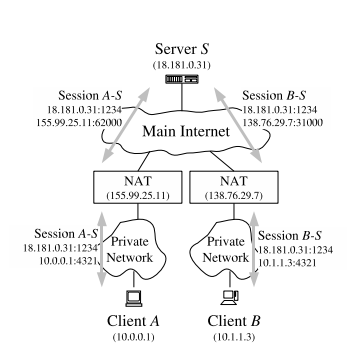
\includegraphics[width=0.5\linewidth]{fig/NAT_Traversal/relaying.png}
        \caption{Travessia de NAT por \textit{relaying}, conforme \citep{ford2005peer}.}
        \label{fig:relaying_server}
\end{figure}

\subsection{Connection Reversal}
\label{sec:connection_reversal}

O \textit{connection reversal} é uma técnica voltada para o caso em que apenas um dos \textit{peers} está atrás de um NAT (cliente A), enquanto o outro possui um endereço IP público (cliente B). O objetivo desse método é fazer com que o cliente atrás do NAT inicie a conexão com o cliente que possui endereço público, o que inverte o sentido original da tentativa de conexão. Para isso, a técnica utiliza um servidor intermediário (\textit{rendezvous point}), cuja função se limita ao registro dos \textit{peers} e à descoberta de seus respectivos endereços IP público e privado.

O processo ocorre da seguinte forma: o cliente A estabelece uma conexão com o servidor S, e o cliente B, ao se registrar, obtém por meio do servidor os endereços IP público e privado do cliente A. Em seguida, o cliente B tenta iniciar uma comunicação direta com o cliente A, utilizando ambos os endereços obtidos. Caso essa tentativa falhe, o cliente B solicita ao servidor S que encaminhe um pedido de conexão ao cliente A pela conexão já ativa entre A e o servidor. Ao receber esse pedido, o cliente A inicia uma nova conexão diretamente com o cliente B. Como o NAT permite conexões iniciadas a partir da rede interna, essa conexão será bem-sucedida desde que não haja filtragem de conexões no lado do cliente B. A Figura~\ref{fig:connection_reversal} ilustra esse processo.

\begin{figure}[!ht]
        \centering
        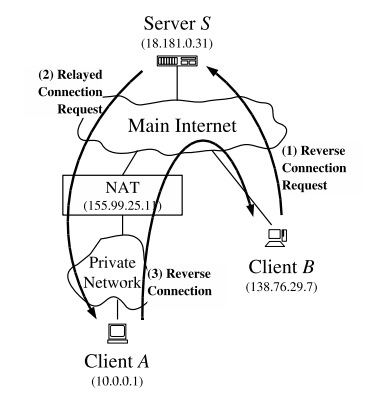
\includegraphics[width=0.5\linewidth]{fig/NAT_Traversal/connection_reversal.png}
        \caption{Travessia de NAT por \textit{connection reversal}, conforme \citep{ford2005peer}.}
        \label{fig:connection_reversal}
\end{figure}

A etapa de reversão, isto é, o encaminhamento do pedido de conexão de B para A por meio do servidor S, seguido do início da conexão por A, só ocorre caso a tentativa de conexão direta de B falhe. Se o NAT de A empregasse EIF (Seção~\ref{sec:nat_classification_by_translation_behavior}), essa tentativa direta teria sucesso para o endereço público do cliente A, e a etapa de reversão seria desnecessária.

\subsection{UDP Hole Punching}
\label{sec:udp_hole_punching}

O \textit{hole punching} sobre UDP (\textit{UDP hole punching}) é, segundo Ford et al. \citep{ford2005peer}, a técnica mais eficaz conhecida para a comunicação P2P. Essa técnica visa estabelecer a comunicação entre dois \textit{peers}, cada um atrás de um NAT, independentemente da topologia existente. Considere o seguinte cenário: dois clientes (A e B), cada um atrás de um NAT (NAT A e NAT B), e um servidor S (\textit{rendezvous server}), em que ambos os NATs são EIM e APDF. Os clientes A e B estabelecem uma sessão com o servidor S, o que cria um mapeamento A:a na tabela do NAT A e um mapeamento B:b na tabela do NAT B, em que A:a e B:b denotam os endereços públicos (endereço IP e porta) mapeados. Os clientes também obtêm, por meio do servidor, esses endereços públicos mapeados.

Caso o cliente A envie uma mensagem para B:b, o NAT B descartará os pacotes, pois o endereço IP e a porta de origem do cliente A não correspondem aos do servidor S, único \textit{host} para o qual o NAT B possui, até então, um mapeamento cuja filtragem permite a recepção de pacotes (o que não ocorreria caso o NAT B fosse EIF). Pelo mesmo motivo, o NAT A descartará as mensagens que o cliente B enviar para A:a.

Diante disso, o cliente A tenta iniciar uma sessão com o cliente B por intermédio do servidor S. O cliente A começa a enviar mensagens para B:b e, ao mesmo tempo, solicita ao servidor S que instrua o cliente B a transmitir pacotes para o endereço público A:a. Ao enviar mensagens para B:b, o cliente A faz com que o NAT A passe a aceitar, no mapeamento A:a, pacotes provenientes de B:b. Da mesma forma, ao enviar mensagens para A:a, o cliente B faz com que o NAT B passe a aceitar, no mapeamento B:b, pacotes provenientes de A:a. Com isso, os dois clientes estabelecem uma sessão direta. A Figura~\ref{fig:udp_hole_punching} ilustra esse cenário.

\begin{figure}[!ht]
        \centering
        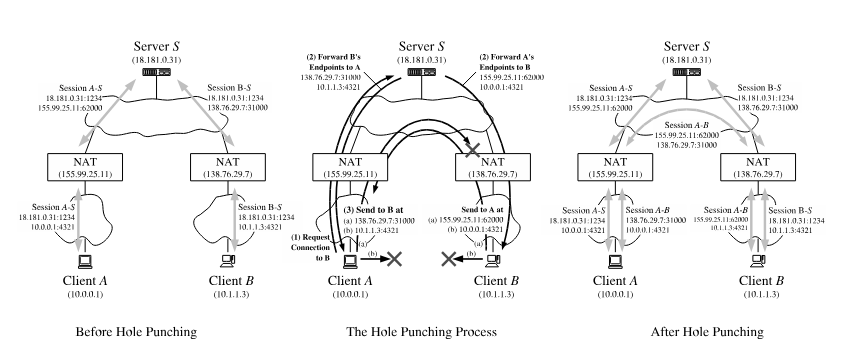
\includegraphics[width=1.0\linewidth]{fig/NAT_Traversal/udp_hole_punching.png}
        \caption{Travessia de NAT por \textit{hole punching} sobre UDP, conforme \citep{ford2005peer}.}
        \label{fig:udp_hole_punching}
\end{figure}

As técnicas de \textit{hole punching} descritas nesta seção dependem de NATs EIM; caso contrário, os clientes não conseguiriam descobrir o endereço público X:x do cliente de destino. Em NATs com mapeamento dependente do destino (EDM, do inglês \textit{Endpoint-Dependent Mapping}), isto é, ADM ou APDM, o endereço X:x seria diferente para cada destino, de modo que o servidor S não conseguiria fornecer aos clientes A e B os endereços públicos que cada um utilizaria na comunicação com o outro.

\subsubsection{UDP Hole Punching Sob o Mesmo NAT}

O \textit{hole punching} atrás do mesmo NAT corresponde ao cenário de topologia em que múltiplos \textit{peers} estão em uma mesma rede privada, sem necessariamente ter conhecimento dessa condição. Nesse cenário, duas técnicas permitem estabelecer a comunicação. Considere o cenário ilustrado na Figura~\ref{fig:udp_hole_punching_same_nat}.

Os clientes A e B inicialmente se conectam ao servidor S e obtêm seus respectivos endereços mapeados. A primeira técnica consiste em aplicar o \textit{hole punching} convencional com esses endereços públicos, o que só terá sucesso caso o dispositivo NAT suporte \textit{hairpinning}.

O \textit{hairpinning} consiste na capacidade de um NAT de encaminhar pacotes entre dois \textit{peers} da mesma rede privada quando um deles os envia ao endereço público mapeado do outro. A Figura~\ref{fig:hairpinning} ilustra esse comportamento.

\begin{figure}[!ht]
        \centering
        \hl{fazer}
 %       \includegraphics[width=1.0\linewidth]{tem que fazer}
        \caption{Técnica de NAT Hairpinning.}
        \label{fig:hairpinning}
\end{figure}

Dessa forma, quando o cliente A envia um pacote para o cliente B, o NAT traduz o endereço público B:b para o endereço privado de B, e o mesmo ocorre quando o cliente B envia um pacote para o cliente A. Entretanto, o suporte a esse comportamento está longe de ser universal: segundo Ford et al. \citep{ford2005peer}, das 335 amostras testadas para \textit{hairpin translation} em UDP, apenas 80 (24\%) o suportaram.

A segunda técnica, que independe do suporte a \textit{hairpinning}, aplica-se quando os endereços privados dos clientes são acessíveis e roteáveis entre eles. Assim como no \textit{connection reversal} (Seção~\ref{sec:connection_reversal}), os \textit{peers} informam ao servidor S tanto o endereço privado quanto o público. Ao receber os endereços do \textit{peer} de destino, cada \textit{peer} envia mensagens simultaneamente para os dois endereços, e o endereço que responder primeiro passa a ser utilizado na conexão.

\begin{figure}[!ht]
        \centering
        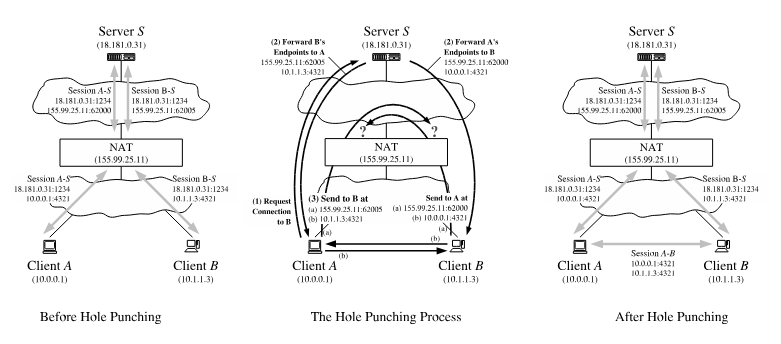
\includegraphics[width=1.0\linewidth]{fig/NAT_Traversal/udp_hole_punching_same_nat.png}
        \caption{Travessia de NAT por \textit{hole punching} sobre UDP atrás de um NAT compartilhado, conforme \citep{ford2005peer}.}
        \label{fig:udp_hole_punching_same_nat}
\end{figure}

\subsubsection{UDP Hole Punching Sob Múltiplos NATs}

Um cenário especialmente relevante na prática, dada a disseminação do \textit{Carrier-Grade NAT} (CGNAT) entre provedores de acesso à Internet (ISP, do inglês \textit{Internet Service Provider}), é o de topologias com múltiplos NATs, descrito no RFC 5128 \citep{rfc5128} e ilustrado na Figura~\ref{fig:udp_hole_punching_multiple_nat}.

Nesse caso, a comunicação se inicia como nas demais situações: os clientes A e B estabelecem conexão com o servidor S. Idealmente, o servidor S conheceria os endereços mapeados pelos NATs A e B; entretanto, esses endereços são privados no domínio de endereçamento do ISP, e os únicos endereços públicos que o servidor S conhece são os do NAT C, ao qual os NATs A e B estão conectados.

Portanto, segundo o RFC 5128, os clientes não têm outra opção senão utilizar os endereços IP públicos mapeados pelo NAT C e visíveis no domínio do servidor S, o que exige que o NAT C suporte \textit{hairpinning}.

\begin{figure}[!ht]
        \centering
        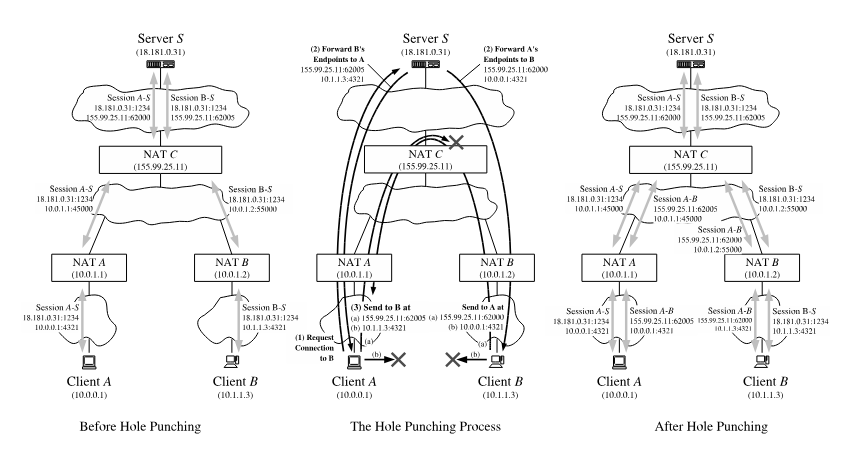
\includegraphics[width=1.0\linewidth]{fig/NAT_Traversal/udp_hole_punching_multiple_nat.png}
        \caption{Travessia de NAT por \textit{hole punching} sobre UDP atrás de múltiplos NATs, conforme \citep{ford2005peer}.}
        \label{fig:udp_hole_punching_multiple_nat}
\end{figure}

\subsubsection{UDP Hole Punching para EDM NAT}
\label{sec:udp_hole_punching_edm}

Algumas tentativas de comunicação P2P deparam-se com NATs mais restritivos, que não implementam EIM, isto é, NATs EDM (Seção~\ref{sec:nat_classification_by_translation_behavior}). Como, nesses NATs, o mapeamento público depende do destino, o servidor S não consegue informar aos \textit{peers} os endereços públicos de seus destinos.

Entretanto, conforme o RFC 5128, é possível analisar o comportamento do NAT na escolha da porta pública. Na maior parte dos casos, o NAT atribui e mapeia portas de forma sequencial, o que permite prever a próxima porta a ser alocada. Por isso, essa técnica de predição de portas (\textit{port prediction}) é frequentemente denominada ``N+1''.

Como nas seções anteriores, os clientes A e B acessam o servidor S e obtêm seus endereços públicos A:a e B:b. Em seguida, o cliente A envia mensagens para a porta prevista de B, B:b+1, e o cliente B envia mensagens para a porta prevista de A, A:a+1. Se ambos os clientes preverem corretamente a próxima porta que o NAT do outro \textit{peer} mapeará, os dois estabelecem a comunicação.

Na prática, essa técnica falha em diversos cenários: se a porta prevista já estiver em uso, se outro \textit{host} gerar um novo mapeamento antes do mapeamento da porta prevista ou se o NAT não atribuir portas de forma sequencial. Além disso, quanto mais níveis de NAT a comunicação precisar atravessar, menor a chance de sucesso, pois aumenta a probabilidade de que outro cliente envie um pacote e ocupe a porta prevista em algum dos níveis intermediários.

Por fim, para combinar essa técnica com as demais, seria necessário identificar previamente o tipo de NAT responsável pela tradução, o que aumentaria a complexidade e a latência do estabelecimento de conexão.

A predição de portas também se aplica ao \textit{hole punching} sobre TCP (Seção~\ref{sec:tcp_hole_punching}). Nesse caso, entretanto, a técnica é ainda mais frágil e sensível a \textit{timing} do que no UDP, o que torna a solução mais instável.

\subsection{TCP Hole Punching}
\label{sec:tcp_hole_punching}

O \textit{hole punching} sobre TCP (\textit{TCP hole punching}), também associado à abertura simultânea de conexões TCP (\textit{TCP simultaneous open}), segue o mesmo princípio do \textit{hole punching} sobre UDP. Entretanto, essa técnica é mais complexa devido ao problema de sincronização envolvido. Assim como no UDP, o NAT mapeia uma conexão TCP por fluxo. No UDP, que não possui o conceito de conexão, um fluxo começa com o envio do primeiro pacote e, como não há um fim explícito, o NAT remove o mapeamento, na maioria dos casos, após um tempo de inatividade (\textit{timeout}). No TCP, um fluxo começa quando o primeiro pacote \texttt{SYN} sai de um dos \textit{peers}, e seu fim é bem definido pelo envio de um pacote \texttt{FIN} ou \texttt{RST}.

O \textit{hole punching} sobre TCP também se baseia no mapeamento por fluxo da tabela NAT. Entretanto, segundo Ford et al. \citep{ford2005peer}, muitos NATs não tratam adequadamente pacotes \texttt{SYN} não solicitados. Ao receber uma conexão TCP externa, isto é, não iniciada pela rede privada, o NAT pode responder com um pacote \texttt{RST}, o que leva o NAT do remetente a remover o mapeamento do fluxo, ou simplesmente descartar o pacote. Ambos os comportamentos impedem o \textit{hole punching} sobre TCP.

Para contornar essa limitação, a técnica emprega o \textit{TCP simultaneous open}, em que ambos os \textit{peers} iniciam as conexões simultaneamente. Considere a mesma topologia da Figura~\ref{fig:udp_hole_punching}. Caso os clientes A e B enviem pacotes \texttt{SYN} ao mesmo tempo, os NATs A e B criam os mapeamentos A:a e B:b para os respectivos destinos. Assim, ao receber um pacote \texttt{SYN} logo após o envio de um \texttt{SYN} próprio, cada NAT interpreta o pacote recebido como uma resposta esperada e permite sua passagem, o que possibilita o início de uma sessão TCP. Entretanto, essa técnica não é confiável em todas as tentativas, justamente por causa da sincronização: caso um dos pacotes chegue ao NAT de destino muito antes do outro, esse NAT pode descartá-lo ou recusá-lo com um pacote \texttt{RST}. Além disso, a máquina de estados do TCP pode entrar em um estado de \textit{timeout} de fim de sessão, o que impede a aceitação de pacotes TCP mesmo que os dois \textit{peers} enviem pacotes \texttt{SYN} consecutivos.

Apesar dessas limitações, Ford et al. \citep{ford2005peer} e o RFC 5128 \citep{rfc5128} afirmam que a maior parte dos NATs permite o \textit{hole punching} sobre TCP por meio do \textit{TCP simultaneous open}, com sucesso em mais de 50\% dos casos. Ford et al. relatam, a partir de testes em uma ampla variedade de NATs, uma taxa de sucesso de 64\%. O RFC 5128 destaca ainda que outros trabalhos, com técnicas mais sofisticadas do que as de Ford et al., obtiveram suporte de até 88\% para o \textit{hole punching} sobre TCP.

\section{Interactive Connectivity Establishment (ICE)}
\label{sec:ice}

O protocolo ICE \citep{rfc8445} realiza a travessia de NAT em comunicações baseadas em UDP. O ICE utiliza o protocolo STUN e, como alternativa (\textit{fallback}), sua extensão TURN para permitir a comunicação entre dois \textit{peers}, cada um atrás de um NAT, por meio da técnica de \textit{hole punching} ou através de servidores \textit{relay}. Antes de descrever o funcionamento do ICE, as subseções a seguir apresentam os mecanismos dos protocolos STUN e TURN.

\subsection{Servidor STUN}
\label{sec:stun_server}

O STUN é um protocolo que outros protocolos utilizam para realizar a travessia de NAT; por si só, ele não constitui uma técnica de travessia, mas uma ferramenta. O STUN fornece o endereço IP e a porta que um NAT alocou para um dispositivo, permite verificar a conectividade entre \textit{endpoints} e atua como mecanismo de \textit{keep-alive}, que mantém ativos os mapeamentos da tabela NAT.

O campo de tipo das mensagens STUN divide-se em dois subcampos: a classe e o método. A classe indica a natureza da mensagem e ocupa 2 bits, o que resulta em quatro classes possíveis:

\begin{itemize}
    \item \textbf{\textit{Request}:} Mensagem que exige resposta e pode ser retransmitida;
    \item \textbf{\textit{Indication}:} Mensagem que não exige resposta;
    \item \textbf{\textit{Success Response}:} Resposta de sucesso a uma \textit{request};
    \item \textbf{\textit{Error Response}:} Resposta de erro a uma \textit{request}.
\end{itemize}

As extensões e aplicações que utilizam o STUN, como o TURN, definem, em geral, seus próprios métodos; o RFC 8489 \citep{rfc8489} define apenas o método \texttt{Binding}. Esse método retorna ao requisitante o endereço IP e a porta públicos observados pelo servidor STUN. Algumas implementações armazenam esses valores, embora o RFC 8489 não exija nem preveja esse armazenamento.

Em relação à segurança, o STUN pode operar sobre UDP, TCP, DTLS (\textit{Datagram Transport Layer Security}) sobre UDP e TLS (\textit{Transport Layer Security}) sobre TCP. Com DTLS ou TLS, a comunicação é cifrada e autenticada conforme esses protocolos. O STUN também prevê um mecanismo de autenticação por usuário e senha, com credenciais de curta ou de longa duração, aplicado a cada mensagem STUN, que pode servir como camada adicional de segurança mesmo com o uso de DTLS ou TLS. O protocolo permite essa autenticação sem DTLS ou TLS, mas essa configuração não é recomendada, pois a comunicação perde as garantias de confidencialidade providas pela criptografia dessas tecnologias.

A Figura~\ref{fig:stun_time_diagram} apresenta o diagrama de tempo do processamento de uma mensagem de método \texttt{Binding} e classe \texttt{Request}, com a respectiva resposta de método \texttt{Binding} e classe \texttt{Success Response}.

\begin{figure}[!ht]
        \centering
        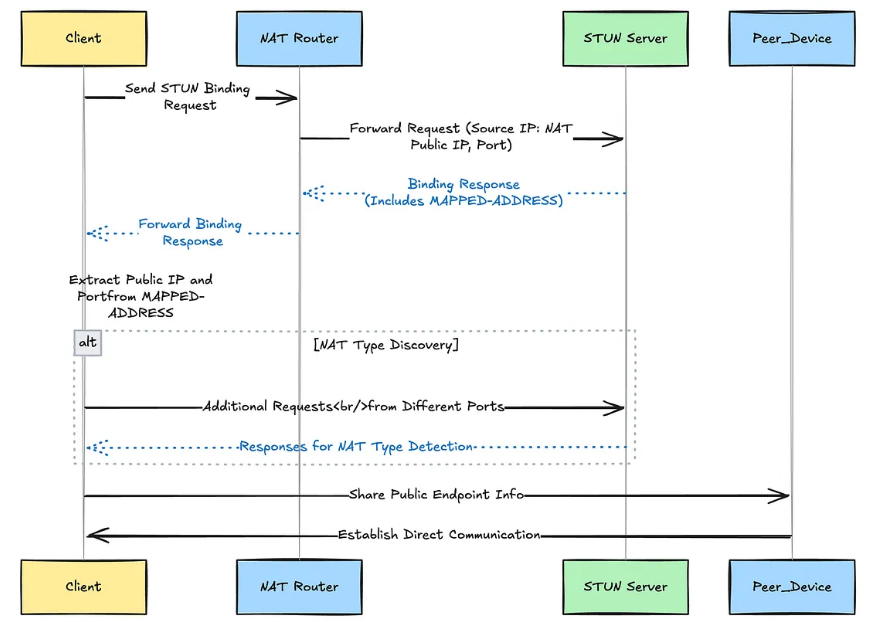
\includegraphics[width=1.0\linewidth]{fig/ICE/stun_time_diagram.png}
        \caption{Diagrama de tempo do STUN, conforme \citep{bordane2024stun}.}
        \label{fig:stun_time_diagram}
\end{figure}

\begin{comment}
CARA IMPORTANTE LEMBRAR O SEGUINTE

Hairpinning permite que de dentro da rede eu acesse o outro peer usando o IP/port público dele descober pelo STUN, isso permite que o holepunching funcione mesmo que os 2 peers estejam abaixo do mesmo NAT

Também importante lembrar onde isso se sobrepõe com aplicações UNSAF do RFC
\end{comment}

\subsection{Servidor TURN}
\label{sec:turn_server}

O TURN é um protocolo desenvolvido para viabilizar a comunicação nos casos em que dois \textit{peers} atrás de NAT não conseguem se comunicar diretamente. Esses casos, descritos nas Seções~\ref{sec:nat_classification_by_translation_behavior} e~\ref{sec:udp_hole_punching}, decorrem das limitações e dos bloqueios de NATs que não implementam EIM. Por isso, diversos trabalhos, como \citep{liao2020turnproxy}, descrevem o TURN como uma solução para os casos de falha do \textit{hole punching}.

O TURN resolve esses cenários por meio de um ponto intermediário, denominado \textit{relay} ou servidor TURN (\textit{TURN server}), que permite que \textit{peers} (\textit{TURN clients}) se comuniquem por meio de um terceiro \textit{host}. O servidor TURN também pode ocultar dos demais \textit{peers} os endereços IP e as portas públicos mapeados; nesse caso, o servidor atua como um \textit{proxy} especializado.

A Figura~\ref{fig:turn_topology} ilustra a topologia entre clientes e servidor TURN. Os clientes podem estar ou não atrás de um NAT, e cada um pode ou não atuar como \textit{TURN client}. O RFC 8656 \citep{rfc8656} define, entre outros, os seguintes endereços de transporte: o endereço do cliente no lado externo do NAT, visto pelo servidor, denomina-se \textit{server-reflexive transport address}; o endereço do servidor utilizado pelos clientes para enviar mensagens TURN denomina-se \textit{TURN server transport address}; e o endereço do \textit{peer}, visto pelo servidor, denomina-se \textit{peer transport address}.

\begin{figure}[!ht]
        \centering
        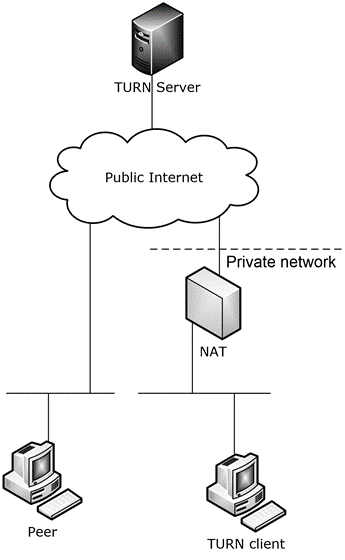
\includegraphics[width=0.4\linewidth]{fig/ICE/turn_topology.png}
        \caption{Exemplo de topologia cliente-servidor TURN, conforme \citep{microsoft2022msturn}.}
        \label{fig:turn_topology}
\end{figure}

O TURN foi projetado para operar como parte do protocolo ICE. Além disso, o TURN é uma extensão do protocolo STUN, e suas mensagens utilizam o formato das mensagens STUN.

Durante a comunicação, as mensagens enviadas de um cliente TURN ao servidor trafegam sobre um protocolo de transporte previamente escolhido. Ao receber um pacote a ser retransmitido, o servidor o desencapsula e o envia ao \textit{peer} de destino em um datagrama UDP. No sentido contrário, ao receber um datagrama UDP do \textit{peer}, o servidor TURN encapsula a mensagem em uma mensagem TURN e a encaminha ao cliente. A Tabela~\ref{tab:turn_transports} resume essa relação.

\begin{table}[htbp]
    \centering
    \begin{tabular}{|l|l|}
        \hline
        \textbf{Cliente TURN $\rightarrow$ Servidor TURN} &
        \textbf{Servidor TURN $\rightarrow$ \textit{Peer}} \\
        \hline
        UDP & UDP \\
        \hline
        TCP & UDP \\
        \hline
        TLS-over-TCP & UDP \\
        \hline
        DTLS-over-UDP & UDP \\
        \hline
    \end{tabular}
    \caption{Protocolos de transporte do TURN, conforme \citep{rfc8656}.}
    \label{tab:turn_transports}
\end{table}

Os clientes solicitam alocações ao servidor TURN por meio de uma requisição \texttt{Allocate}. O servidor autentica essas requisições com o mecanismo de autenticação do STUN e, em resposta, reserva um endereço próprio, denominado \textit{relayed transport address}. Esse endereço passa a ser o ponto de contato pelo qual os \textit{peers} enviam tráfego ao cliente, e o servidor encaminha ao cliente os dados recebidos nesse endereço. A Figura~\ref{fig:turn_time_diagram} apresenta o diagrama de tempo do processo de alocação em um servidor TURN.

\begin{figure}[!ht]
        \centering
        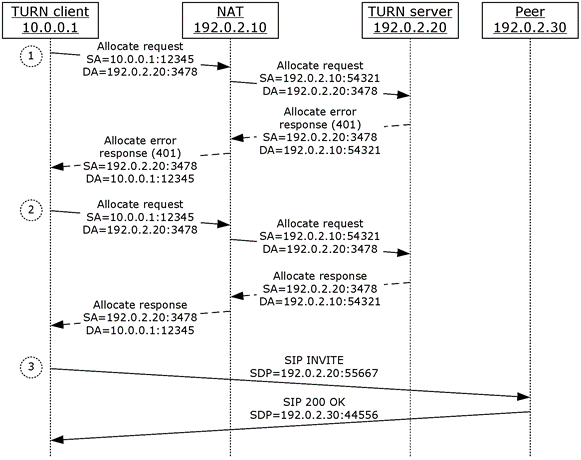
\includegraphics[width=0.8\linewidth]{fig/ICE/turn_time_diagram.png}
        \caption{Diagrama de tempo do TURN, conforme \citep{microsoft2022msturnexamples}.}
        \label{fig:turn_time_diagram}
\end{figure}

Para garantir a segurança e impedir o uso do TURN para contornar (\textit{bypass}) \textit{firewalls}, o servidor implementa o conceito de permissões: antes de aceitar tráfego de um \textit{peer} específico endereçado ao \textit{relayed transport address} do cliente, o servidor exige que o cliente tenha instalado explicitamente uma permissão para esse \textit{peer}. Esse conceito é análogo ao comportamento de filtragem dos NATs (Seção~\ref{sec:nat_classification_by_translation_behavior}). Cada permissão funciona como uma concessão temporária (\textit{lease}) e expira após 5 minutos caso o cliente não a renove.

O servidor TURN oferece dois mecanismos de envio e retransmissão de dados:

\begin{itemize}
    \item \textbf{\textit{Indications}:} As \textit{indications} são mensagens no formato STUN, conforme a Seção~\ref{sec:stun_server}, e dividem-se em dois tipos: \textit{Send Indication} e \textit{Data Indication}. A \textit{Send Indication} transporta dados do cliente ao servidor, que os retransmite ao \textit{peer}; a \textit{Data Indication} transporta ao cliente os dados que o servidor recebeu do \textit{peer};
    \item \textbf{\textit{Channels}:} Os canais utilizam um formato simplificado de mensagem, denominado \textit{ChannelData}, que dispensa o cabeçalho STUN e reduz o consumo de banda. Para criar um canal, o cliente envia uma requisição \texttt{ChannelBind} que associa um número de canal de 2 bytes, escolhido pelo próprio cliente, a um \textit{peer} específico; esse número, somado a um campo de tamanho de 2 bytes, forma o cabeçalho de 4 bytes de cada mensagem \textit{ChannelData}. O canal opera nos dois sentidos (do cliente ao \textit{peer} e do \textit{peer} ao cliente) e permanece ativo por 10 minutos caso o cliente não o renove, o dobro da duração de uma permissão, o que garante que o canal não expire antes dela.
\end{itemize}

\subsection{Protocolo ICE}

O protocolo ICE, definido no RFC 8445 \citep{rfc8445}, combina as vantagens das técnicas de travessia de NAT apresentadas anteriormente, de modo a reduzir a complexidade e maximizar o uso de comunicações P2P em diferentes topologias. O ICE opera nativamente sobre fluxos de dados (\textit{streams}) em UDP, utiliza os protocolos STUN e TURN na seleção de endereços e suporta \textit{hosts} com um ou múltiplos endereços IP (\textit{multihomed}).

O ICE baseia-se na coleta de endereços candidatos para a comunicação entre os dois \textit{peers}; cada combinação de candidatos representa uma possível tentativa de comunicação. Esses candidatos incluem o endereço local do \textit{host} (ou \textit{gateway}) e os endereços obtidos por meio dos protocolos auxiliares do ICE (STUN e TURN). A Figura~\ref{fig:ice_candidates} ilustra esses candidatos. Cada \textit{gateway} executa seu próprio agente ICE. Os candidatos obtidos e os pares selecionados referem-se aos caminhos de comunicação desses \textit{gateways}, e não aos endereços dos sensores ou atuadores associados a eles.

\begin{figure}[!ht]
        \centering
        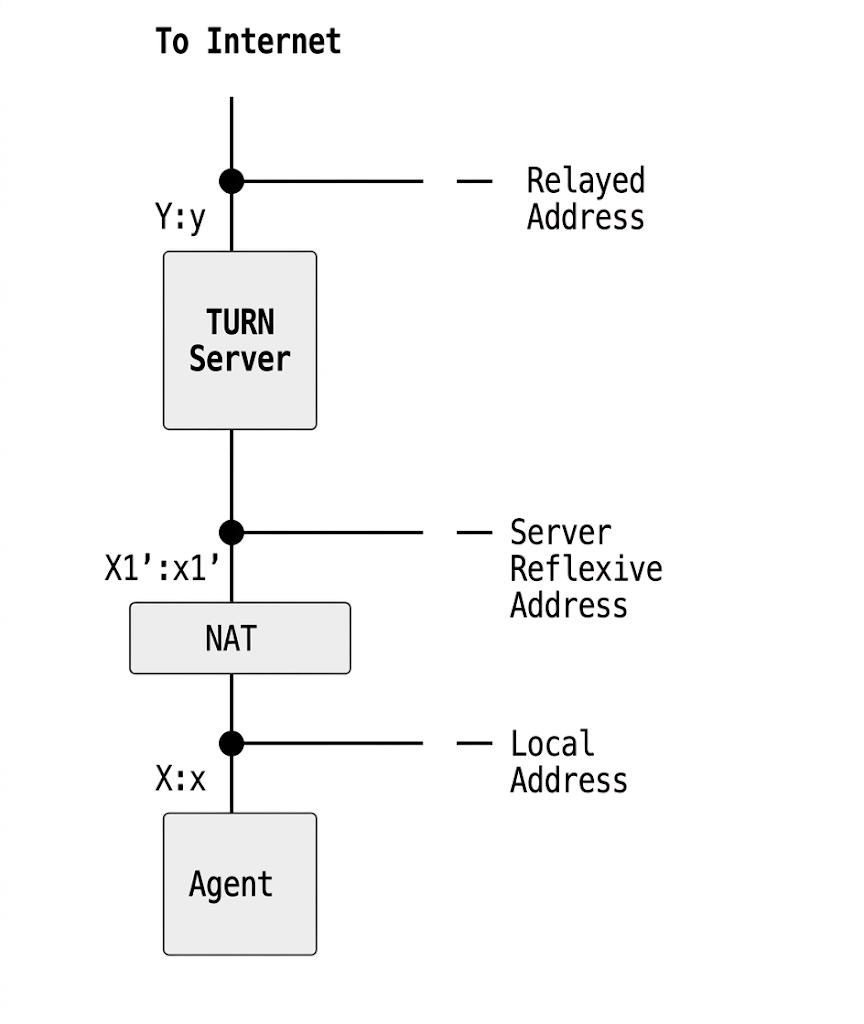
\includegraphics[width=0.6\linewidth]{fig/ICE/ice_addresses.png}
        \caption{Endereços de candidatos ICE, baseado em \citep{rfc8445}.}
        \label{fig:ice_candidates}
\end{figure}

Os candidatos apresentados na figura são:

\begin{itemize}
    \item \textbf{\textit{Local Address}:} Endereço IP da interface de rede do \textit{host};
    \item \textbf{\textit{Server Reflexive Address}:} Endereço IP público que o NAT atribui ao \textit{host}, obtido por meio do STUN;
    \item \textbf{\textit{Relayed Address}:} Endereço IP que o servidor TURN (\textit{relay}) aloca para o \textit{host}.
\end{itemize}

Há ainda o \textit{Peer Reflexive Address}, que corresponde ao endereço do \textit{host} observado pelo outro \textit{peer} e que pode diferir dos endereços observados pelos servidores STUN e TURN. O ICE descobre esse endereço durante as verificações de conectividade (\textit{connectivity checks}) e o adiciona à lista de candidatos. Em resumo, o ICE busca descobrir o maior número possível de endereços capazes de representar um \textit{peer}, a fim de encontrar ao menos um que viabilize a comunicação.

Cada candidato possui um atributo denominado \textit{base}, que representa o endereço a partir do qual o agente ICE (\textit{ICE agent}) efetivamente envia pacotes ao utilizar esse candidato. Para os candidatos \textit{host}, \textit{server-reflexive} e \textit{peer-reflexive}, a base corresponde ao \textit{local address}. Para o candidato \textit{relayed}, a base é o próprio candidato, isto é, o endereço alocado pelo servidor TURN, pois é o servidor, e não o \textit{host}, quem envia os pacotes a partir desse endereço.

Após a descoberta dos candidatos, o agente ICE os ordena por prioridade e os troca com o outro \textit{peer} por meio de um servidor de sinalização. A prioridade de cada candidato resulta de uma fórmula em que cada tipo de candidato possui um peso específico. O ICE não define o servidor de sinalização, que pode ser qualquer canal confiável entre os \textit{peers}. De posse dos candidatos de ambos os lados, o agente ICE forma pares de candidatos (\textit{candidate pairs}) e inicia as verificações de conectividade por meio de mensagens STUN \texttt{Binding} (\textit{request} e \textit{response}).

O algoritmo do ICE compreende as seguintes etapas, detalhadas a seguir:

\begin{itemize}
    \item \textbf{Ordenação de candidatos:} O agente ICE ordena os pares de candidatos por prioridade;
    \item \textbf{Verificações de conectividade:} Os agentes verificam cada par de candidatos por meio de mensagens STUN \texttt{Binding}; ao receber uma requisição de verificação, o \textit{peer} responde com uma \textit{Binding Success Response}.
\end{itemize}

\subsubsection{Verificações de Conectividade do ICE}
\label{sec:ice_connectivity_checks}

As verificações de conectividade avaliam os pares de candidatos para selecionar o melhor par da lista de prioridades e confirmar que ao menos um deles viabiliza a comunicação. O uso de \textit{relay} praticamente garante a comunicação; entretanto, por ser a opção menos eficiente, os candidatos \textit{relayed} recebem a menor prioridade e funcionam como última alternativa.

As verificações de conectividade seguem um \textit{handshake} de quatro mensagens (\textit{4-way handshake}), o que corresponde a dois RTTs (\textit{Round Trip Time}), conforme ilustra a Figura~\ref{fig:connectivity_check_4way_handshake}. O agente ICE executa as verificações na ordem da lista de prioridade dos pares de candidatos, denominada \textit{checklist}. Os \textit{triggered checks} otimizam esse processo: ao receber uma verificação de um par, o agente envia imediatamente uma verificação no sentido oposto, o que acelera a descoberta de pares válidos. O agente insere os pares que passam na verificação, denominados \textit{valid pairs}, em uma lista própria, a \textit{valid list}. Ao final do processo, o ICE seleciona um par por componente; assim, há mais de um par selecionado apenas quando a comunicação possui mais de um componente de \textit{stream}, como no uso do RTP (\textit{Real-time Transport Protocol}) e do RTCP (\textit{RTP Control Protocol}), protocolos que são utilizados no padrão WebRTC descritos na Seção~\ref{sec:webrtc}, em cenários sem multiplexação de componentes (Estes protocolos podem ou não multiplexar diferentes \textit{streams} no mesmo endereço).

\begin{figure}[!ht]
        \centering
        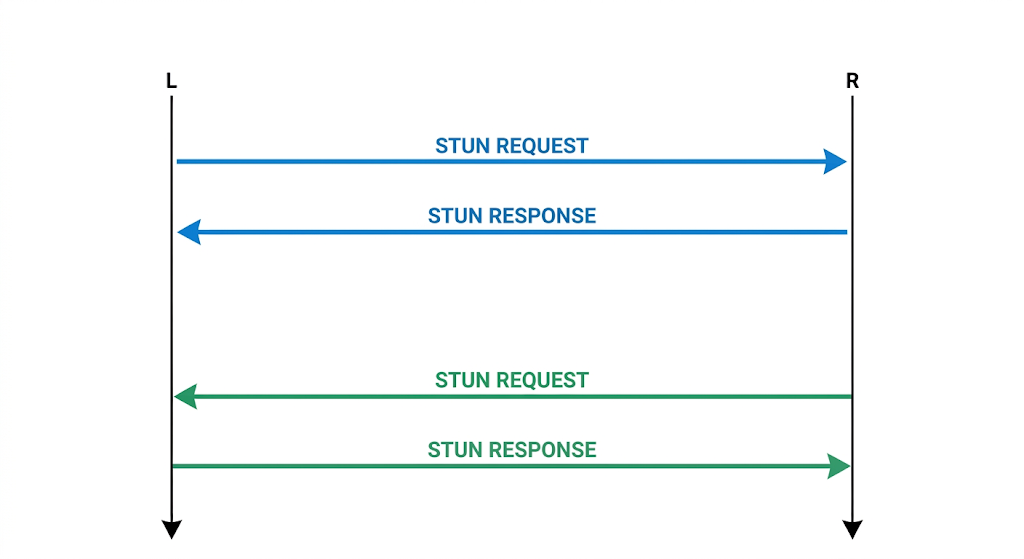
\includegraphics[width=0.7\linewidth]{fig/ICE/4way_handshake.png}
        \caption{\textit{4-way handshake} das verificações de conectividade do ICE, baseado em \citep{rfc8445}.}
        \label{fig:connectivity_check_4way_handshake}
\end{figure}

Durante as verificações de conectividade, o ICE atribui um papel a cada \textit{peer}: um atua como agente controlador (\textit{controlling agent}) e o outro, como agente controlado (\textit{controlled agent}). Essa atribuição define a condição de parada das verificações, que prosseguem até que o agente controlador encontre um par válido. Em seguida, o agente controlador envia uma requisição STUN \texttt{Binding} com o atributo \texttt{USE-CANDIDATE}, que informa ao agente controlado o par a ser utilizado para a transmissão de dados a partir desse momento (Figura~\ref{fig:4way_and_attribute}).

\begin{figure}[!ht]
        \centering
        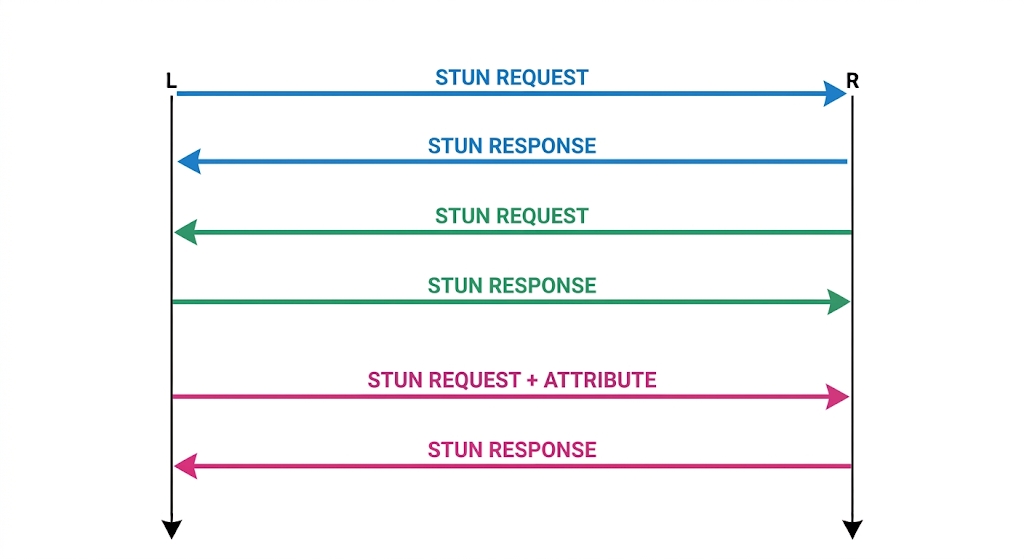
\includegraphics[width=0.7\linewidth]{fig/ICE/4way_and_attribute.png}
        \caption{\textit{4-way handshake} das verificações de conectividade do ICE com o atributo \texttt{USE-CANDIDATE}, baseado em \citep{rfc8445}.}
        \label{fig:4way_and_attribute}
\end{figure}

Como os pacotes do \textit{4-way handshake} podem ser perdidos, o agente ICE os retransmite em intervalos determinados. A perda de um pacote pode decorrer do comportamento de filtragem do NAT (Seção~\ref{sec:nat_classification_by_translation_behavior}) ou de características do meio. O primeiro motivo é o relevante, pois o ICE testa justamente a permissividade dos NATs. Portanto, para que o agente considere um par inválido apenas quando um NAT restritivo o bloqueia, a retransmissão é necessária, de modo a descartar perdas causadas por problemas de temporização, sincronização ou limitações do meio. Dois parâmetros definidos pelo protocolo, Ta e RTO (\textit{Retransmission Timeout}), regem as políticas de transmissão e retransmissão das verificações de conectividade:

\begin{itemize}
    \item \textbf{Ta:} Intervalo mínimo entre o envio de verificações de conectividade. Como pode haver mais de uma verificação em andamento, retransmissões podem ocorrer enquanto o agente gera novas verificações. O RFC 8445 sugere Ta de 50~ms, mas admite outros valores, desde que respeitem o limite mínimo de 5~ms;
    \item \textbf{RTO:} Tempo de espera antes de uma retransmissão. O protocolo STUN define esse parâmetro \citep{rfc8489}, cujo valor dobra a cada nova retransmissão. O RFC 8445 define o cálculo do RTO inicial, mas admite outros cálculos, desde que o valor inicial seja maior ou igual a 500~ms.
\end{itemize}

\section{Chownat}
\label{sec:chownat}

O Chownat é uma aplicação desenvolvida por Kamkar \citep{kamkar2004chownat} que aplica as técnicas de travessia de NAT apresentadas na Seção~\ref{sec:udp_hole_punching} para estabelecer uma conexão entre dois \textit{peers}, cada um atrás de um NAT, e encapsular tráfego TCP em UDP. Para isso, a aplicação divide os \textit{peers} em cliente e servidor: o cliente sempre inicia a conexão, e o servidor aguarda a mensagem do cliente.

\subsection{Arquitetura do Chownat}

O Chownat possui uma arquitetura que permite o tunelamento de serviços TCP sobre UDP. Para isso, a aplicação mantém abertos dois \textit{sockets}: um UDP, que realiza o \textit{hole punching}, e um TCP, que gerencia o serviço TCP. A Figura~\ref{fig:chownat_architecture} ilustra essa arquitetura.

\begin{figure}[!ht]
        \centering
        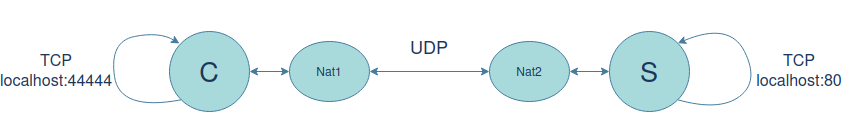
\includegraphics[width=1.0\linewidth]{fig/chownat/chownat_architecture.png}
        \caption{Diagrama de arquitetura do Chownat.}
        \label{fig:chownat_architecture}
\end{figure}

As portas indicadas na Figura~\ref{fig:chownat_architecture} são apenas ilustrativas e correspondem a um exemplo de tunelamento do tráfego TCP de um serviço HTTP (porta 80); o Chownat, entretanto, suporta qualquer serviço TCP. Este trabalho utiliza a versão 0.07 do Chownat \citep{kamkar2004chownatv07}.

O \textit{socket} UDP utiliza uma porta local escolhida e envia pacotes ao endereço IP público do \textit{peer} de destino. Para simplificar o cenário, o Chownat utiliza a mesma porta nos dois \textit{peers}, cuja porta padrão é a 2222. Essa porta é também a utilizada no \textit{hole punching}: como o Chownat não dispõe da infraestrutura de servidores e de descoberta de candidatos do ICE (Seção~\ref{sec:ice}), o endereço IP público do \textit{peer} deve ser configurado previamente, e o NAT deve preservar a porta na tradução.

Por exemplo, se o \textit{socket} UDP do cliente estiver vinculado a cIP:2222, o NAT1 precisará traduzi-lo para nat1IP:2222, de modo que o \textit{peer} servidor S consiga enviar pacotes para nat1IP:2222. Da mesma forma, o servidor terá o endereço sIP:2222, e o NAT2 precisará traduzi-lo para nat2IP:2222. Esse é o cenário necessário para que a comunicação e o \textit{hole punching} do Chownat funcionem. Com a infraestrutura de servidores do ICE, essa rigidez seria evitada, pois os endereços públicos seriam descobertos dinamicamente, e a porta pública não precisaria coincidir com a porta vinculada ao \textit{socket} UDP.

O \textit{socket} TCP vincula-se ao endereço \textit{localhost} e a uma porta que depende da função do \textit{peer}; assim, todo o tráfego TCP ocorre internamente no \textit{peer}. No servidor, a porta corresponde à do serviço associado (no exemplo da Figura~\ref{fig:chownat_architecture}, a porta 80 do serviço HTTP). No cliente, o Chownat utiliza qualquer porta livre (no exemplo, a porta 44444), para a qual o cliente do serviço TCP direciona todo o seu tráfego. Como o transporte TCP ocorre apenas localmente, o Chownat coleta o \textit{payload} (conteúdo) que o cliente TCP envia ao \textit{socket} e transporta apenas esse \textit{payload} via UDP, sem os segmentos de controle do TCP. Da mesma forma, o Chownat coleta o \textit{payload} recebido pelo \textit{socket} UDP e o entrega ao serviço local por meio do \textit{socket} TCP. Esse processo constitui o tunelamento de TCP sobre UDP.

Embora utilize técnicas associadas ao modelo P2P, o Chownat não adota necessariamente esse modelo, pois seu transporte segue a lógica cliente-servidor (Seção~\ref{sec:network_architecture_models}). Como o Chownat apenas fornece o meio de comunicação entre os \textit{peers} e não define o papel de cada nó em relação à informação transmitida, a arquitetura geral depende do serviço executado sobre ele.

\subsection{Protocolo Chownat}
\label{sec:chownat_protocol}

O protocolo do Chownat é simples e recupera pacotes perdidos por meio de pacotes de controle, além de prover as operações básicas necessárias à comunicação. O protocolo também deve viabilizar o \textit{hole punching} sobre UDP. Dessa forma, ele se divide em duas etapas: a etapa de conexão e a etapa de comunicação. Antes de descrevê-las, esta seção apresenta o cabeçalho e os tipos de pacotes utilizados.

\subsubsection{Tipos de Pacote do Chownat}

O Chownat utiliza dois tipos de pacotes, de controle e de dados, que compartilham o mesmo formato de cabeçalho. A análise do código-fonte da versão 0.07 \citep{kamkar2004chownatv07} indica que esse cabeçalho possui 3 bytes, no formato ilustrado na Figura~\ref{fig:header_chownat}.

\begin{figure}[!ht]
        \centering
        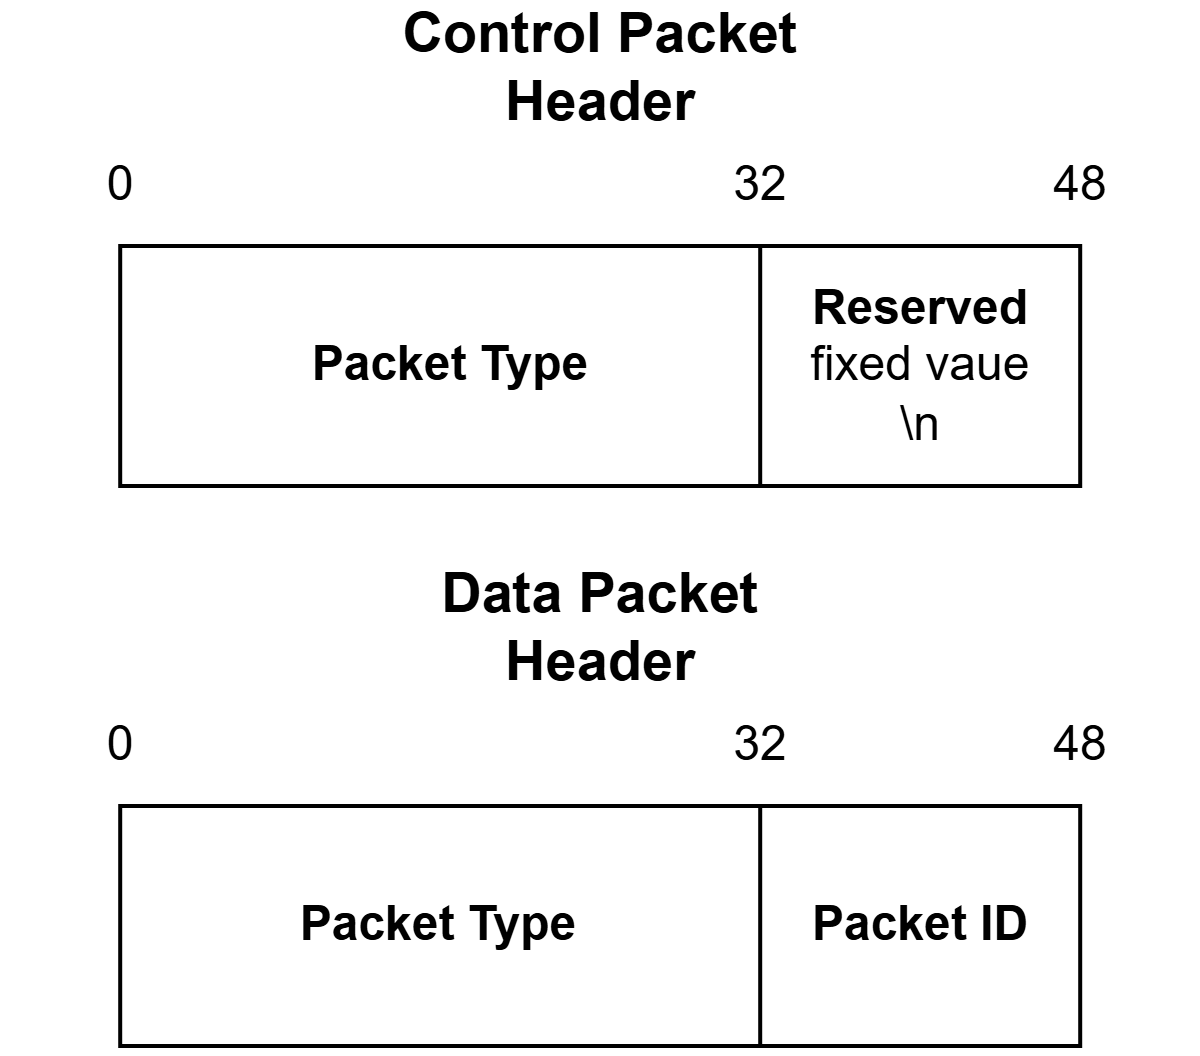
\includegraphics[width=0.6\linewidth]{fig/chownat/chownat_headers.png}
        \caption{Cabeçalhos do Chownat.}
        \label{fig:header_chownat}
\end{figure}

O campo \textit{packet type} abrange 5 tipos de pacotes, distribuídos entre controle e dados, descritos a seguir.

\paragraph{Pacotes de Controle}

\begin{itemize}
    \item \textbf{01:} Pacote de início de conexão, que o cliente Chownat envia para iniciar uma nova conexão e o processo de \textit{hole punching};
    \item \textbf{02:} Pacote de fim de conexão, que o cliente ou o servidor Chownat envia para encerrar uma conexão;
    \item \textbf{03:} Pacote de \textit{keep-alive}, que o servidor utiliza para iniciar o processo de \textit{hole punching} e que ambos os \textit{peers} utilizam para manter o mapeamento do endereço público em seus respectivos NATs.
\end{itemize}

\paragraph{Pacotes de Dados}

\begin{itemize}
    \item \textbf{08:} Pacote de requisição de retransmissão, que ambos os \textit{peers} podem utilizar para solicitar a retransmissão de pacotes; o campo \textit{packet ID} indica a partir de qual pacote o \textit{peer} necessita da retransmissão;
    \item \textbf{09:} Pacote de envio de dados, que ambos os \textit{peers} utilizam para enviar o \textit{payload} do serviço TCP; o campo \textit{packet ID} funciona como número de sequência do pacote.
\end{itemize}

\subsubsection{Etapa de Conexão do Protocolo Chownat}
\label{sec:chownat_connection}

A etapa de conexão realiza o \textit{hole punching} e um \textit{3-way handshake} que confirma a conexão entre os dois \textit{peers}. Cada \textit{peer} segue um fluxo distinto, e a combinação das ações de ambos viabiliza a comunicação; por isso, a comunicação exige um cliente e um servidor, e não ocorre entre dois clientes ou entre dois servidores.

O servidor inicialmente vincula (\textit{bind}) os \textit{sockets} TCP e UDP e aguarda o cliente por um intervalo fixo de 5~s. Sempre que esse intervalo se esgota, o servidor envia um pacote de \textit{keep-alive}, que gera o mapeamento do fluxo de comunicação no NAT e, assim, define o endereço IP e a porta públicos. Quando o \textit{hole punching} ocorre, o servidor recebe uma requisição de conexão do cliente e inicia o \textit{3-way handshake}. Se o \textit{handshake} for bem-sucedido, o servidor conecta seu \textit{socket} TCP local ao serviço TCP desejado (no exemplo, o serviço HTTP na porta 80) e conclui a etapa de conexão.

O cliente também vincula inicialmente os \textit{sockets}; entretanto, em vez de aguardar uma mensagem, como o servidor, o cliente aguarda uma conexão TCP em \texttt{localhost:Porta Servico} e atua como servidor TCP local (na Figura~\ref{fig:chownat_architecture}, \texttt{PortaServico} corresponde à porta 44444). O cliente local do serviço (no exemplo, o cliente HTTP) inicia essa comunicação ao direcionar seu tráfego para \texttt{localhost:PortaServico}. O cliente Chownat, então, aceita a conexão TCP e tenta se conectar ao servidor Chownat. Se o servidor Chownat já tiver enviado o primeiro pacote de \textit{keep-alive} e o NAT já tiver mapeado o endereço e a porta públicos, o \textit{3-way handshake} se inicia e, se bem-sucedido, conclui a etapa de conexão.

Em síntese, no Chownat há um cliente e um servidor UDP para o \textit{hole punching}, enquanto, no TCP, os papéis se invertem: o cliente Chownat atua como servidor TCP e recebe requisições TCP externas à aplicação, e o servidor Chownat atua como cliente TCP, inicia a conexão com o serviço TCP local e redireciona a ele o conteúdo recebido nos pacotes UDP, originalmente enviado pelo cliente TCP conectado ao cliente Chownat.

\subsubsection{Etapa de Comunicação do Protocolo Chownat}

A etapa de comunicação realiza o tunelamento de dados TCP sobre UDP nos dois sentidos. No sentido cliente-servidor, o cliente Chownat coleta o \textit{payload} recebido em seu \textit{socket} TCP local, no qual atua como servidor, e o encaminha pelo túnel UDP ao servidor Chownat, que o entrega ao serviço TCP local ao qual está conectado como cliente. No sentido servidor-cliente, o servidor Chownat coleta as respostas do serviço TCP e as encaminha pelo túnel UDP ao cliente Chownat, que as entrega ao cliente TCP local. A Figura~\ref{fig:chownat_architecture} ilustra esse fluxo com o exemplo de uma requisição HTTP, detalhado a seguir.

No exemplo, o cliente HTTP no \textit{peer} do cliente Chownat envia uma requisição para \texttt{localhost:PortaServico} (porta 44444), na qual o cliente Chownat a recebe como servidor TCP local. De posse do \textit{payload} dessa requisição, o cliente Chownat o encaminha pelo túnel UDP estabelecido com o servidor Chownat ao final da etapa de conexão (Seção~\ref{sec:chownat_connection}).

Ao receber esse pacote, o servidor Chownat encaminha o \textit{payload} ao serviço HTTP local pela conexão TCP que ele próprio estabeleceu, como cliente, ao final da etapa de conexão. O Chownat continua a repassar os pacotes nesse fluxo até que uma das partes encerre a conexão: o cliente HTTP local, ao final da requisição, ou o serviço HTTP local, por qualquer motivo (pacote inválido, serviço indisponível ou outro erro).

Como cada \textit{peer} gerencia a conexão TCP localmente, os segmentos de controle do TCP não trafegam pelo túnel UDP e, portanto, não existem na rede, o que torna a troca de informações mais rápida e reduz o uso de banda. Em contrapartida, como os mecanismos de controle do TCP não atuam sobre o túnel, o próprio protocolo Chownat assume esse controle e provê as garantias possíveis, como retransmissão de pacotes e ordem de chegada.

O Chownat garante a ordem de chegada e a retransmissão de pacotes por meio de um identificador único no cabeçalho dos pacotes de dados. O receptor detecta a perda de um pacote pela chegada de um pacote fora de ordem: ao receber um pacote cujo identificador não corresponde ao próximo esperado, o receptor descarta esse pacote e solicita a retransmissão a partir do identificador esperado, o que indica a perda dos pacotes intermediários.

Por exemplo, suponha que o cliente Chownat envie três pacotes ao servidor Chownat: o primeiro chega normalmente, o segundo se perde e o terceiro chega fora de ordem. Como o identificador do terceiro pacote não corresponde ao esperado (o do segundo), o servidor descarta esse pacote e solicita a retransmissão a partir do segundo; o cliente, então, reenvia o segundo e o terceiro pacotes. Caso a perda ocorra no último pacote de uma sequência, nenhum pacote subsequente chega fora de ordem para revelar a perda, e o mecanismo do Chownat não a detecta; nesses casos, cabe ao próprio serviço TCP tunelado perceber a ausência de resposta e solicitar a retransmissão na camada de aplicação.

Para manter o mapeamento no NAT e a disponibilidade da comunicação, o Chownat utiliza as mensagens de \textit{keep-alive}. Além de servirem de base para o início da comunicação, essas mensagens impedem que o mapeamento expire por inatividade na tabela NAT. O Chownat envia um pacote de \textit{keep-alive} sempre que permanece 5~s sem receber pacotes.

O Chownat apresenta limitações. Além da perda de parte dos recursos de controle do TCP, o protocolo implementa a desconexão apenas parcialmente: embora o protocolo preveja a desconexão, a implementação original da versão 0.07 apenas entra em \textit{loop}, e uma camada superior, como o sistema operacional, precisa finalizar o processo. Assim, para executar novamente o serviço TCP, é necessário um novo processo de conexão, com nova etapa de \textit{hole punching}, o que restringe a aplicação do Chownat. Na adaptação proposta neste trabalho, as aplicações e os serviços TCP locais são executados nos hosts que representam os gateways. Essa organização fornece o ponto de integração entre os dados das aplicações locais e o transporte externo.

\begin{comment}
    
\section{Web Real-Time Communication (WebRTC)}
\label{sec:webrtc}

Segundo o RFC 8825 \citep{RFC8825}, o WebRTC é um conjunto de protocolos que permite a comunicação de áudio, vídeo e dados entre \textit{peers} pelo caminho mais curto entre eles. O padrão foi desenvolvido inicialmente para o tráfego de tempo real entre navegadores, sobretudo videochamadas, e posteriormente se estendeu a outros tipos de aplicação.

Conforme \citep{WebRTCOrg} e \citep{Sequeira2017WebRTCHistory}, o WebRTC tem origem em tecnologias da GIPS (\textit{Global IP Solutions}), empresa adquirida pelo Google em 2010, que tornou essas tecnologias abertas em 2011. Atualmente, o W3C (\textit{World Wide Web Consortium}) e o IETF mantêm o padrão com escopos distintos \citep{RFC8825}: o W3C define uma API padronizada em JavaScript para a comunicação entre navegadores, enquanto o IETF define os protocolos de forma independente dessa API, de modo que quaisquer \textit{peers} que implementem o mesmo conjunto de especificações possam se comunicar entre si.

Como seu escopo não envolve comunicação Web, este trabalho concentra-se na abordagem do IETF, sobretudo do ponto de vista arquitetural. Ainda assim, a arquitetura concebida para o tráfego Web é útil para diversos outros tipos de comunicação. Por isso, este trabalho adota como principal referência o livro de DuBois e Ivov \citep{WebRTCForTheCurious}, que privilegia os aspectos técnicos e normativos do WebRTC e, portanto, se alinha ao escopo deste projeto.

DuBois e Ivov \citep{WebRTCForTheCurious} refinam a distinção entre W3C e IETF ao propor uma divisão terminológica entre \textit{protocolo WebRTC} e \textit{API WebRTC}: o protocolo WebRTC corresponde à comunicação bidirecional entre dois \textit{peers}, enquanto a API constitui um nível de abstração sobre o protocolo que permite que desenvolvedores o utilizem. Este trabalho adota essa nomenclatura, salvo indicação contrária.

\subsection{Protocolo WebRTC}
\label{sec:webrtc_protocol}

O protocolo WebRTC compõe-se de etapas sequenciais: cada etapa só começa após a conclusão bem-sucedida da anterior, condição necessária para garantir o transporte. Segundo DuBois e Ivov \citep{WebRTCForTheCurious}, essas etapas são:

\begin{itemize}
    \item \textit{Signaling} (sinalização);
    \item \textit{Connecting} (conexão);
    \item \textit{Securing} (segurança);
    \item \textit{Communicating} (comunicação).
\end{itemize}

A Seção~\ref{sec:webrtc_architecture} descreve cada uma dessas etapas, que dependem de um ou mais protocolos para sua conclusão. Assim, o WebRTC baseia-se em um conjunto de técnicas e protocolos já consolidados. A Figura~\ref{fig:webrtc_protocols} apresenta os protocolos utilizados por um \textit{peer} WebRTC.

\begin{figure}[!ht]
        \centering
        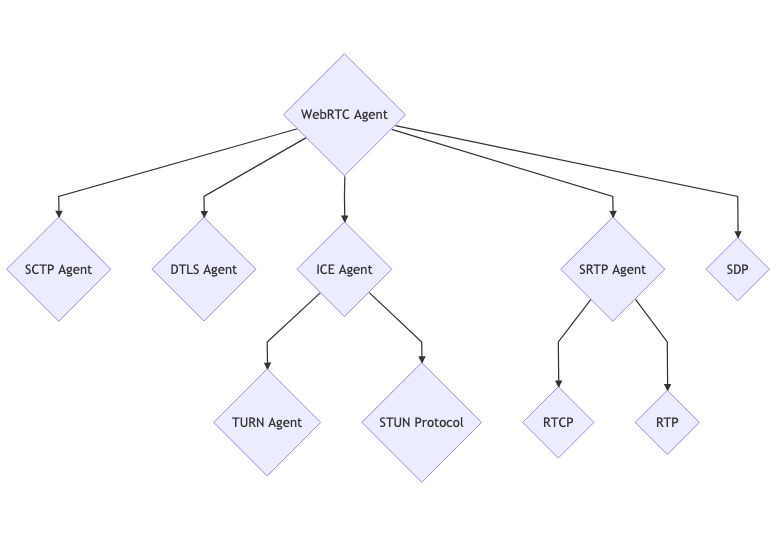
\includegraphics[width=1.0\linewidth]{fig/WebRTC/webrtc_protocol_tree.png}
        \caption{Árvore de dependência dos protocolos do WebRTC, conforme \citep{WebRTCForTheCurious}.}
        \label{fig:webrtc_protocols}
\end{figure}

\subsection{Arquitetura do WebRTC}
\label{sec:webrtc_architecture}

A arquitetura do protocolo WebRTC segue as etapas descritas na Seção~\ref{sec:webrtc_protocol} e pode ser vista, em muitos aspectos, como uma arquitetura híbrida (Seção~\ref{sec:hybrid_peer_to_peer_model}): a etapa inicial de descoberta de endereços segue o modelo cliente-servidor, enquanto a comunicação posterior entre os \textit{peers}, direta ou por meio de \textit{relay}, segue o modelo P2P. A Figura~\ref{fig:webrtc_architecture} ilustra essa arquitetura.

Neste trabalho, a arquitetura do WebRTC serve como referência para as etapas de sinalização e estabelecimento de conectividade por meio do ICE. A comunicação entre os \textit{gateways} utiliza QUIC (Capítulo~\ref{chap:quic}, que integra transporte e segurança no estabelecimento da conexão. A solução não utiliza a API WebRTC de navegador, os canais de dados SCTP ou os mecanismos de transmissão de áudio e vídeo descritos nas subseções seguintes.

\begin{figure}[!ht]
        \centering
        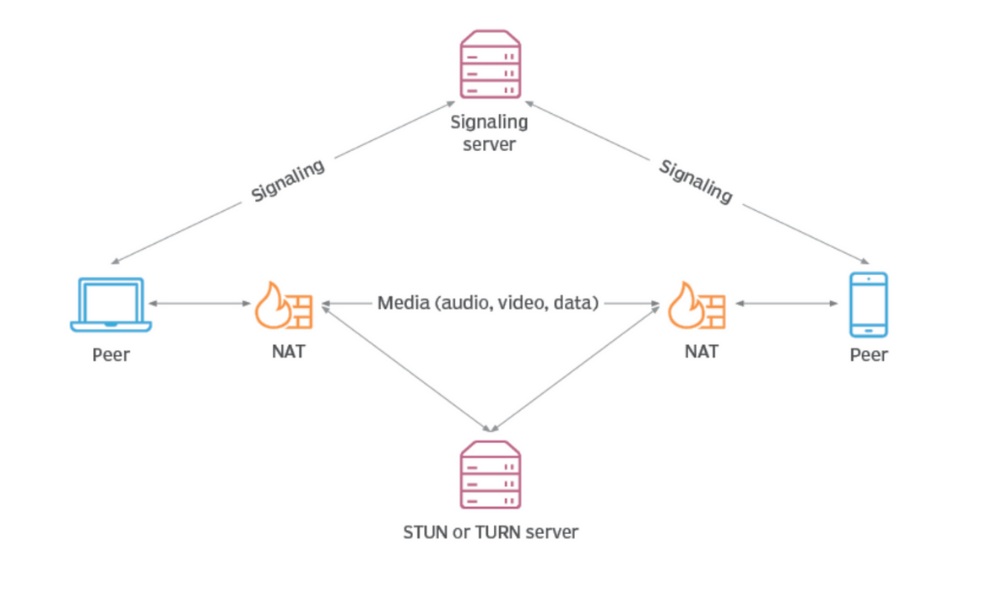
\includegraphics[width=1.0\linewidth]{fig/WebRTC/webrtc_architecture.png}
        \caption{Visão geral da arquitetura do WebRTC, conforme \citep{nugroho2026webrtcwebsocket}.}
        \label{fig:webrtc_architecture}
\end{figure}

\subsubsection{Signaling}
\label{sec:signaling}

A sinalização é a etapa inicial da conexão do protocolo WebRTC. Essa etapa é necessária porque, ao iniciar uma nova instância de conexão WebRTC, denominada agente WebRTC por DuBois e Ivov \citep{WebRTCForTheCurious}, o agente não possui nenhuma informação sobre o \textit{peer} de destino e, portanto, precisa de um meio de troca de mensagens para localizá-lo. O WebRTC não define um protocolo ou serviço para essa troca de mensagens, cuja escolha cabe à aplicação.

Para a sinalização, o protocolo WebRTC utiliza o SDP (\textit{Session Description Protocol}). Como o SDP não foi projetado especificamente para o WebRTC, esta seção não o aborda em seu escopo completo e apresenta apenas os conceitos necessários para compreender seu uso na sinalização do WebRTC.

\paragraph{SDP}

O SDP é um protocolo que padroniza a troca de informações em sessões multimídia. O RFC 2327 \citep{rfc2327} definiu originalmente o SDP, o RFC 4566 \citep{rfc4566} o revisou e, mais recentemente, o RFC 8866 \citep{rfc8866} o consolidou. O protocolo baseia-se em descritores no formato chave-valor (\texttt{<Type>=<Value>}), organizados em descritores de sessão e de mídia. Os descritores de mídia descrevem os fluxos de áudio, vídeo e dados oferecidos, com seus respectivos atributos (\textit{codecs}, credenciais do ICE, impressão digital do certificado, entre outros). A Figura~\ref{fig:sdp_example} apresenta o diagrama de fluxo do SDP.

\begin{figure}[!ht]
        \centering
        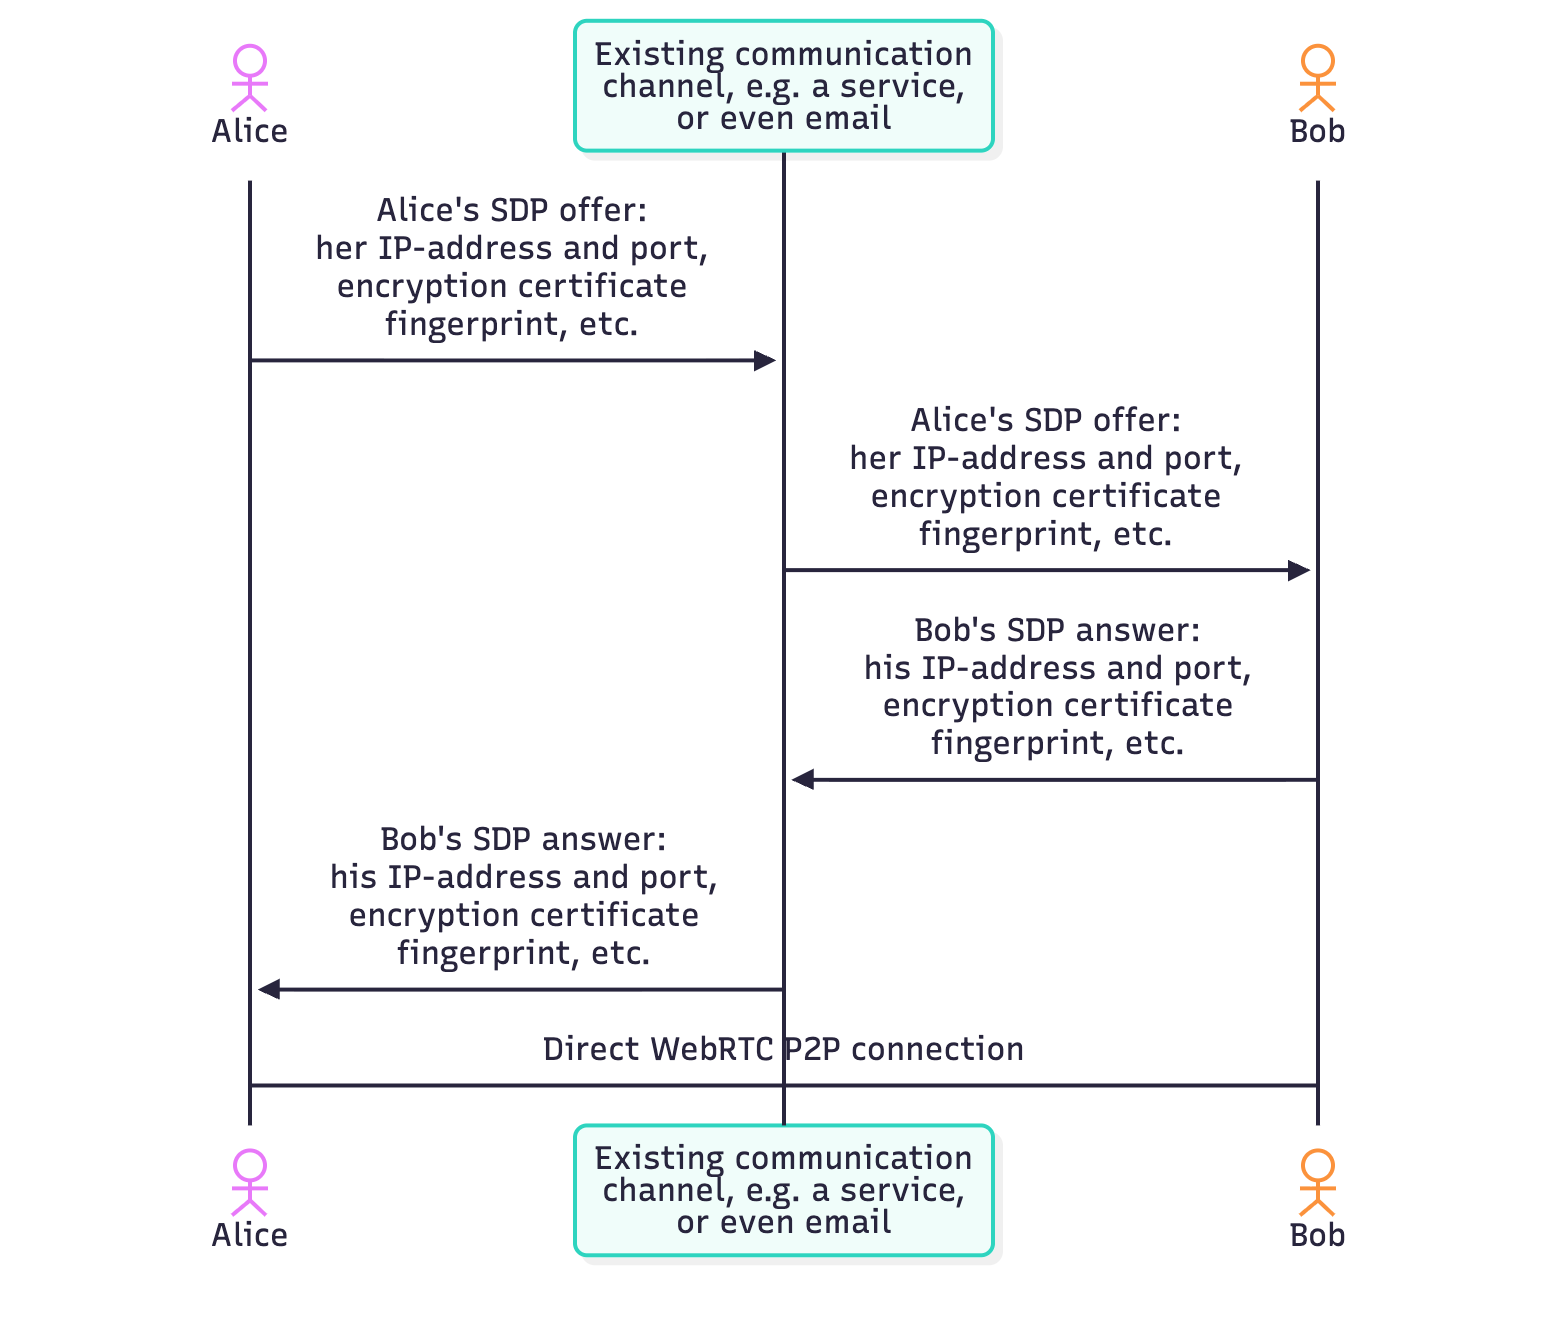
\includegraphics[width=1.0\linewidth]{fig/WebRTC/sdp_example.png}
        \caption{Diagrama de fluxo do SDP, conforme \citep{WebRTCForTheCurious}.}
        \label{fig:sdp_example}
\end{figure}

No contexto do WebRTC, os agentes utilizam o SDP segundo o modelo de oferta e resposta (\textit{offer/answer model}): um agente envia uma oferta com sua descrição de sessão, e o outro responde com uma descrição que aceita apenas os fluxos de seu interesse.

\subsubsection{Connecting}
\label{sec:connecting}

Conforme a Seção~\ref{sec:hybrid_peer_to_peer_model}, o WebRTC adota um modelo de arquitetura híbrido \citep{WebRTCForTheCurious}: emprega o modelo cliente-servidor na troca inicial de informações com os servidores STUN e TURN (Seção~\ref{sec:ice}) e, em seguida, adota o modelo P2P entre os agentes WebRTC.

A necessidade do ICE e dos servidores STUN e TURN decorre justamente da comunicação P2P, sujeita aos problemas descritos na Seção~\ref{sec:nat_problem_for_p2p_communication} e às características do NAT descritas na Seção~\ref{sec:network_address_translator}. As condições que viabilizam as técnicas de travessia no WebRTC são as mesmas descritas na Seção~\ref{sec:udp_hole_punching}.

Na prática, cada agente WebRTC coleta seus próprios candidatos (endereços locais, refletidos via STUN e, quando necessário, retransmitidos via TURN) e os troca com o agente remoto por meio dos atributos \texttt{a=candidate} da descrição de sessão (\textit{Session Description}), durante a sinalização (Seção~\ref{sec:signaling}). De posse dos candidatos de ambos os lados, o agente ICE forma pares de candidatos e testa a conectividade entre eles; os pares que trocam tráfego com sucesso tornam-se pares válidos (\textit{Valid Candidate Pairs}). Em seguida, o agente controlador escolhe um desses pares válidos e o nomeia como \textit{Nominated Pair}. Os agentes controlador e controlado realizam, então, uma última rodada de comunicação bidirecional sobre esse par; se bem-sucedida, o \textit{Nominated Pair} torna-se o \textit{Selected Candidate Pair}, utilizado durante o restante da sessão. A conclusão desse processo de seleção encerra a etapa de conexão do protocolo WebRTC. A Seção~\ref{sec:ice} detalha esse processo.

\subsubsection{Securing}
\label{sec:securing}

A segurança do protocolo WebRTC decorre da autenticação e da cifragem da conexão com o agente WebRTC remoto por meio do DTLS, em conjunto com um protocolo de comunicação como o SRTP (\textit{Secure Real-time Transport Protocol}), de modo que terceiros não tenham acesso às informações transmitidas. Entretanto, como a autenticação do DTLS depende da impressão digital do certificado trocada durante a sinalização (Seção~\ref{sec:signaling}), o protocolo não protege contra ataques \textit{man-in-the-middle} caso o canal de sinalização seja comprometido.

\paragraph{DTLS}

O DTLS \citep{RFC6347} é um protocolo projetado para ser o mais semelhante possível ao TLS, porém adaptado a datagramas. O TLS opera sobre o TCP e, portanto, depende de um transporte que garanta a entrega e a ordem dos pacotes. Como muitas aplicações passaram a utilizar o UDP e precisavam das mesmas garantias de autenticação e cifragem que o TLS oferece sobre o TCP, o IETF desenvolveu o DTLS.

Assim como o TLS, o DTLS realiza a troca das chaves utilizadas na criptografia e verifica os certificados apresentados no \textit{handshake}. No WebRTC, o agente compara o \textit{hash} do certificado apresentado durante o \textit{handshake} DTLS com a impressão digital (\textit{fingerprint}) do certificado trocada previamente via SDP, na sinalização (Seção~\ref{sec:signaling}).

\subsubsection{Communicating}
\label{sec:webrtc_communicating}

Segundo o RFC 8825 \citep{RFC8825}, a comunicação de um agente WebRTC abrange três tipos de conteúdo: áudio, vídeo e dados, cada um com características e protocolos próprios. A comunicação de áudio e vídeo ocorre em tempo real, um dos principais focos do WebRTC.

A etapa de comunicação ocorre após o estabelecimento da segurança (Seção~\ref{sec:securing}) e utiliza um protocolo de transporte. O WebRTC pode utilizar os seguintes protocolos de transporte:

\begin{itemize}
    \item \textbf{RTP e RTCP:} O RTP \citep{RFC3550} transporta informações de tempo real, como áudio e vídeo. Além dos dados, o RTP fornece números de sequência, marcas de tempo (\textit{timestamps}) e monitoramento de entrega; entretanto, não protege contra perda de pacotes nem garante a entrega em ordem ou qualquer recurso de QoS (\textit{Quality of Service}), o que exige, quando aplicável, outros protocolos que forneçam essas garantias. O RTCP constitui a camada de controle do RTP: gerencia a QoS e transmite informações sobre a sessão entre os \textit{peers}. Ambos os protocolos operam, em geral, sobre UDP;
    \item \textbf{SRTP e SRTCP:} O SRTP e o SRTCP (\textit{Secure RTCP}) \citep{RFC3711} são as versões seguras do RTP e do RTCP e garantem cifragem, autenticação e integridade. O SRTP utiliza dois níveis de chave: uma chave mestra (\textit{master key}), obtida por um mecanismo externo de estabelecimento de chaves, como o DTLS, e chaves de sessão, derivadas da chave mestra e usadas na cifragem dos dados de uma sessão. Os algoritmos utilizados incluem o AES (\textit{Advanced Encryption Standard}) em modo contador (AES-CM, \textit{Counter Mode}) e o HMAC-SHA1 (\textit{Hash-based Message Authentication Code} com \textit{Secure Hash Algorithm 1});
    \item \textbf{SCTP:} O SCTP (\textit{Stream Control Transmission Protocol}) \citep{RFC4960}, atualizado pelo RFC 9260 \citep{RFC9260}, é um protocolo de transporte que opera diretamente sobre o IP. O SCTP foi desenvolvido originalmente para transportar mensagens de sinalização de redes PSTN (\textit{Public Switched Telephone Network}) e passou a ser utilizado em aplicações mais amplas, como o WebRTC, no qual transmite dados sem requisitos de tempo real e opera encapsulado em DTLS sobre UDP. O SCTP é orientado a conexão, garante a entrega e, diferentemente do TCP, permite múltiplos fluxos (\textit{streams}) em uma mesma associação, o que evita o bloqueio de cabeça de fila (\textit{head-of-line blocking}) entre fluxos. O SCTP também oferece suporte nativo a \textit{multihoming}, isto é, a \textit{hosts} com múltiplos endereços IP e rotas disponíveis.
\end{itemize}

\subsection{WebRTC API}

A API WebRTC expõe ao desenvolvedor uma interface central, \texttt{RTCPeerConnection}, que representa a sessão WebRTC como um todo. Por meio dessa interface, o desenvolvedor adiciona fluxos de mídia com o método \texttt{addTrack}, que cria um novo fluxo RTP a ser transmitido, ou abre um canal de dados com o método \texttt{createDataChannel}, que inicializa uma associação SCTP sob demanda.

A descoberta dos endereços remotos ocorre por meio da troca de descrições de sessão. O método \texttt{createOffer} gera uma descrição do estado local do \textit{peer}, que a aplicação envia ao \textit{peer} remoto por um mecanismo externo de sinalização. Ao recebê-la, o \textit{peer} remoto a aplica e responde com uma descrição gerada pelo método \texttt{createAnswer}. Após ambos os lados aplicarem as respectivas descrições remotas, a comunicação P2P pode ser estabelecida. O método \texttt{addIceCandidate} permite incorporar, a qualquer momento, candidatos adicionais descobertos ao longo do processo.

Além disso, a API expõe um conjunto de \textit{callbacks} que notificam a aplicação sobre eventos relevantes da sessão, como o recebimento de uma nova sessão ou a mudança no estado de conectividade.

\end{comment}
\chapter{QUIC}
\label{chap:quic}

O QUIC \citep{rfc8999, rfc9000} é um protocolo de transporte desenvolvido para reduzir a latência, melhorar a eficiência e aumentar a confiabilidade das comunicações na Internet. Diferentemente da pilha tradicional, que combina TCP e TLS em camadas separadas, o QUIC opera sobre o UDP, o que facilita sua implantação em redes existentes e sua implementação no espaço de usuário. Além disso, o QUIC integra o \textit{handshake} do TLS~1.3 ao seu próprio \textit{handshake} de transporte \citep{rfc9001}. Essa integração permite estabelecer uma conexão segura em um único RTT (\textit{Round-Trip Time}), ou em zero RTT na retomada de sessão, enquanto a combinação de TCP e TLS exige dois RTTs com TLS~1.3 ou três com TLS~1.2.

O QUIC também define seu próprio identificador de conexão, o \textit{Connection ID}. No TCP, uma conexão é identificada pela quádrupla formada pelos endereços IP e pelas portas de origem e destino, de modo que a alteração de qualquer um desses valores interrompe a conexão. O QUIC, por sua vez, identifica a conexão pelo \textit{Connection ID}, o que permite mantê-la ativa após uma mudança no caminho de rede, como na migração de um dispositivo de uma rede Wi-Fi para uma rede celular, sem a necessidade de restabelecê-la. Esse mecanismo é denominado \textit{Connection Migration}.

\section{Recursos do QUIC utilizados na proposta}

Na infraestrutura proposta, o QUIC é executado nos \textit{gateways} e transporta os dados das aplicações TCP locais por meio de \textit{streams}. O ICE realiza a descoberta e a seleção dos caminhos de comunicação. Assim, o estabelecimento da conexão QUIC constitui uma etapa do processo completo, que também envolve a sinalização e as verificações de conectividade.

A implementação permite o uso de 0-RTT e de migração de conexão, mas esses recursos não foram avaliados explicitamente nos experimentos. Sua utilização permanece condicionada à disponibilidade de caminhos de comunicação viabilizados pelo ICE, incluindo os mecanismos de travessia de NAT necessários. Portanto, os resultados apresentados não caracterizam os ganhos de latência do 0-RTT nem a continuidade da comunicação durante uma migração.

A abordagem adotada utiliza ICE para estabelecer o caminho de comunicação, em vez da variante de \textit{hole punching} baseada em migração de conexão discutida neste capítulo na Seção \ref{sec:quic_hole_punching}. Os detalhes da integração entre QUIC e ICE são apresentados no Capítulo~\ref{chap:implementation}.

\section{História do QUIC}

O desenvolvimento do QUIC foi motivado pelas limitações da pilha tradicional TCP/TLS/HTTP \citep{marx2020quic}, ilustrada na Figura~\ref{fig:tcp_http_stack}. Embora o HTTP/2 tenha introduzido a multiplexação de fluxos sobre uma única conexão, ele ainda depende do TCP, que entrega os bytes estritamente em ordem. Assim, a perda de um único segmento bloqueia a entrega dos dados de todos os fluxos multiplexados até a sua retransmissão, problema conhecido como \textit{Head-of-Line Blocking}. Além disso, \textit{middleboxes}, como NATs e \textit{firewalls}, inspecionam e, por vezes, modificam o cabeçalho TCP, descartando pacotes com opções desconhecidas, o que dificulta a evolução do protocolo. A implementação do TCP no núcleo do sistema operacional também retarda a adoção de novas funcionalidades. Por fim, mudanças de mapeamento de endereço realizadas pelos próprios NATs, como o \textit{NAT rebinding}, interrompem conexões TCP, pois estas são identificadas pela quádrupla de endereços e portas.

\begin{figure}[!ht]
    \centering
    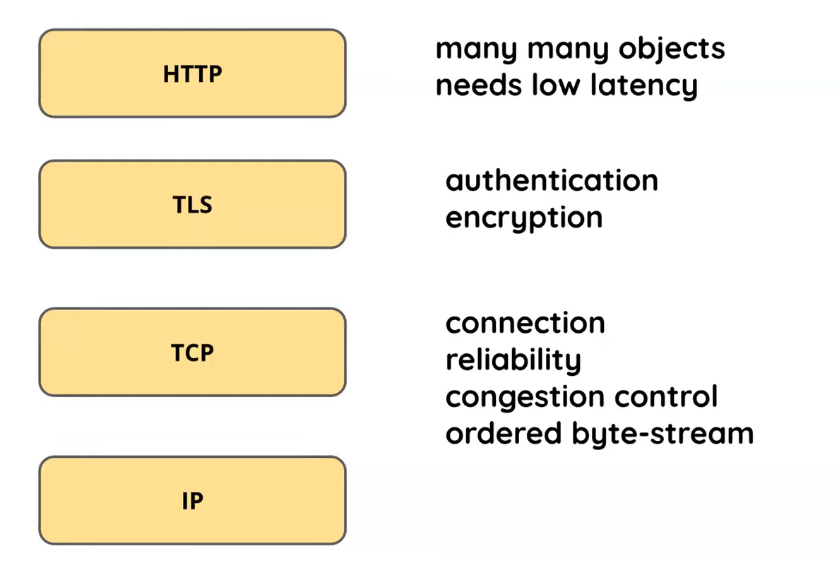
\includegraphics[width=0.7\textwidth]{fig/QUIC/tcp_http_stack.png}
    \caption{Pilha tradicional TCP/TLS/HTTP. Fonte: adaptado de \citep{marx2020quic}.}
    \label{fig:tcp_http_stack}
\end{figure}

A latência é um fator crítico para aplicações como \textit{streaming} de vídeo, navegação \textit{web} interativa e sistemas de tempo real, nas quais pequenas reduções no tempo de resposta melhoram a experiência do usuário. O QUIC foi projetado para superar as limitações descritas acima, oferecendo um protocolo de transporte mais flexível e com menor latência no estabelecimento de conexões.

Entre as principais características do QUIC, destacam-se:

\begin{itemize}
\item Integração com o TLS~1.3, que torna obrigatória a cifragem e a autenticação de todo o tráfego \citep{rfc9001};
\item Estabelecimento de conexão em 1-RTT e retomada de sessão em 0-RTT;
\item Múltiplos fluxos (\textit{streams}) independentes em uma mesma conexão, o que elimina o \textit{Head-of-Line Blocking} entre fluxos;
\item Detecção de perdas e controle de congestionamento implementados no espaço de usuário, com números de pacote monotonicamente crescentes que eliminam a ambiguidade nas retransmissões \citep{rfc9002};
\item Identificadores de conexão (\textit{Connection IDs}), que permitem a migração da conexão entre redes;
\item Proteção de cabeçalho, que cifra metadados como o número de pacote;
\item Suporte a protocolos de aplicação, como o HTTP/3, que exploram essas características.
\end{itemize}

\subsection{GQUIC (Google QUIC)}

O GQUIC foi a implementação original do QUIC, desenvolvida pelo Google a partir de 2012 com o objetivo de melhorar o desempenho do tráfego HTTPS \citep{marx2020quic}. Diferentemente da versão padronizada, o GQUIC utilizava um protocolo criptográfico próprio, o QUIC Crypto, em vez do TLS. Implantado de forma experimental nos serviços do Google, o GQUIC representava, em 2017, mais de 30\% do tráfego de saída da empresa, o que demonstrou na prática que um protocolo baseado em UDP com segurança integrada reduz a latência das conexões \textit{web}.

A arquitetura do GQUIC, ilustrada na Figura~\ref{fig:gquic_stack}, já incorporava conceitos posteriormente adotados pelo QUIC padronizado, como a multiplexação de fluxos, a criptografia integrada ao transporte e o estabelecimento de conexão com menos RTTs.

\begin{figure}[!ht]
    \centering
    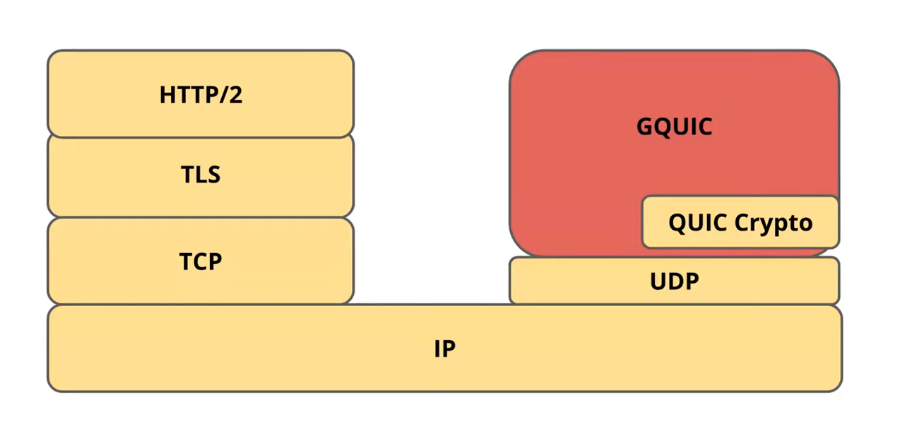
\includegraphics[width=0.7\textwidth]{fig/QUIC/gquic_stack.png}
    \caption{Arquitetura do GQUIC. Fonte: adaptado de \citep{marx2020quic}.}
    \label{fig:gquic_stack}
\end{figure}

\subsection{IQUIC (IETF QUIC)}

Em 2016, a IETF (\textit{Internet Engineering Task Force}) criou o grupo de trabalho QUIC, com o objetivo de padronizar o protocolo a partir da experiência obtida com o GQUIC. A versão resultante é denominada IETF QUIC, ou IQUIC. Durante a padronização, o protocolo recebeu diversas alterações, entre elas a substituição do QUIC Crypto pelo \textit{handshake} do TLS~1.3, novos formatos de cabeçalho, identificadores de conexão de tamanho variável escolhidos por cada \textit{endpoint}, a proteção do número de pacote e a definição de fluxos unidirecionais e bidirecionais. A padronização também separou o protocolo de transporte do mapeamento do HTTP, o que deu origem ao HTTP/3.

O resultado desse processo foi a primeira versão padronizada do protocolo, o QUICv1, publicada em 2021 \citep{rfc9000}, que serve de base para o HTTP/3. A Figura~\ref{fig:quic_stack} mostra a pilha de protocolos com o QUIC, na qual o protocolo de transporte incorpora funcionalidades antes distribuídas entre o TCP e o TLS.

\begin{figure}[!ht]
    \centering
    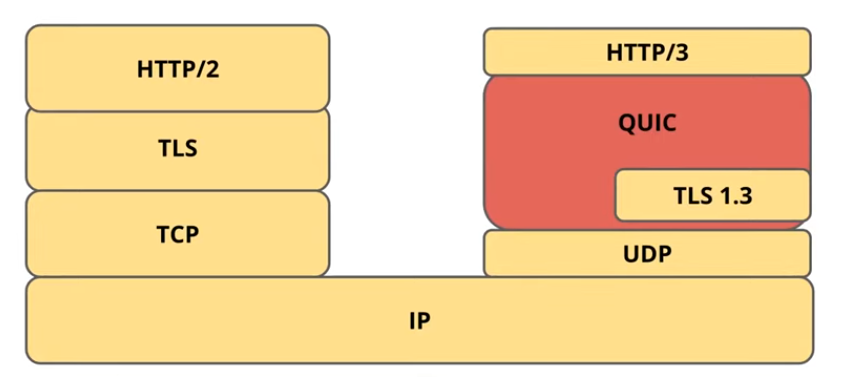
\includegraphics[width=0.7\textwidth]{fig/QUIC/quic_stack.png}
    \caption{Pilha de protocolos utilizando QUIC. Fonte: adaptado de \citep{marx2020quic}.}
    \label{fig:quic_stack}
\end{figure}

\section{Pacotes do QUIC}
\label{sec:quic_packets}

O QUIC define dois formatos de pacote \citep{rfc9000}: os pacotes com \textit{long header} e os pacotes com \textit{short header}. Cada pacote transporta um ou mais \textit{frames}, que são as unidades de informação do protocolo e podem conter dados de aplicação, como os \textit{frames} \texttt{STREAM}, ou informações de controle, como os \textit{frames} \texttt{ACK}. Os pacotes QUIC são transportados em datagramas UDP, e um mesmo datagrama pode conter vários pacotes QUIC, mecanismo denominado \textit{coalescing}. Como o \textit{short header} não possui campo de tamanho, um pacote com esse cabeçalho deve ser o último do datagrama. A Figura~\ref{fig:quic_encapsulation_packet} ilustra essa estrutura.

\begin{figure}[!ht]
    \centering
    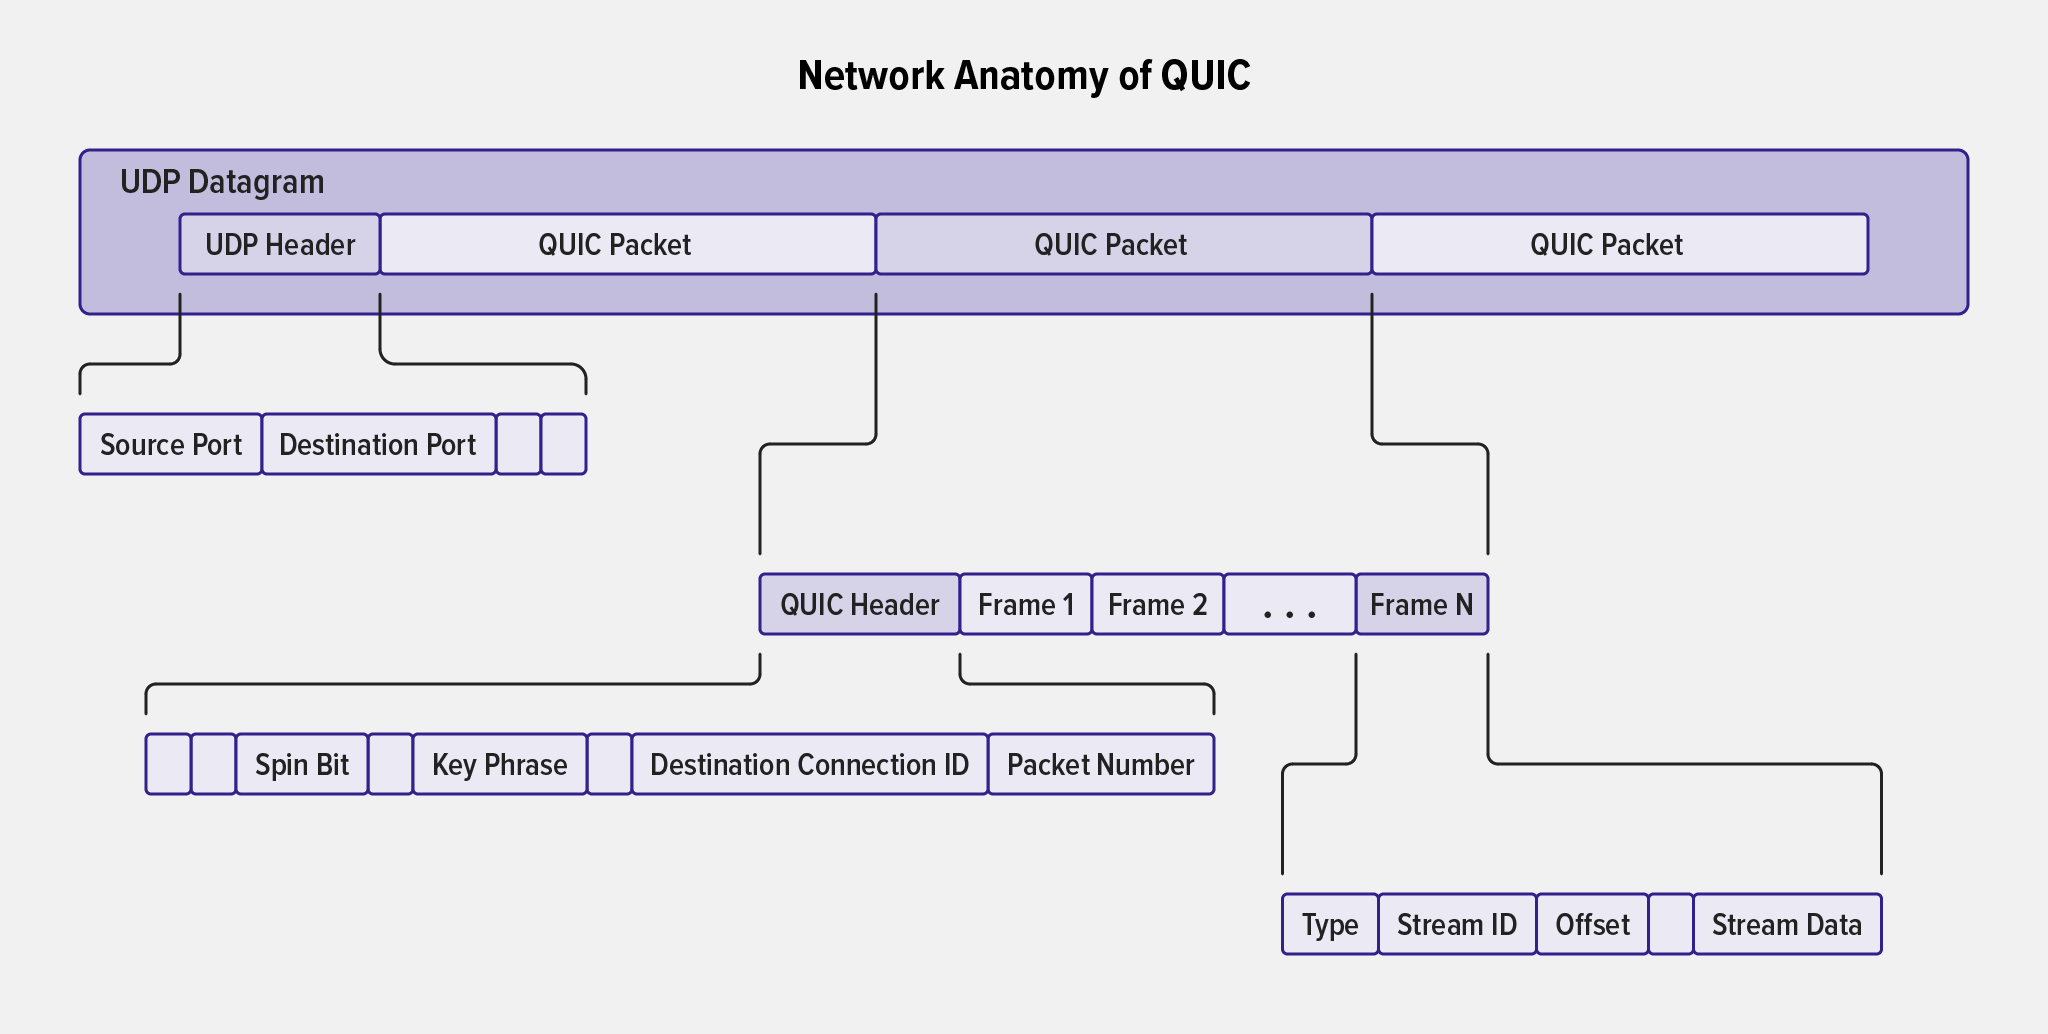
\includegraphics[width=0.9\textwidth]{fig/QUIC/quic_encapsulation_packet.png}
    \caption{Encapsulamento de pacotes QUIC em um datagrama UDP. Fonte: adaptado de \citep{f5_quic_http3}.}
    \label{fig:quic_encapsulation_packet}
\end{figure}


Cada formato de cabeçalho se subdivide em tipos de pacote, e cada tipo cumpre uma função em uma etapa específica da conexão. Os pacotes com \textit{long header} compreendem os tipos \texttt{Initial}, \texttt{0-RTT}, \texttt{Handshake} e \texttt{Retry}, utilizados durante o estabelecimento da conexão, enquanto o \textit{short header} possui um único tipo, o \texttt{1-RTT}, utilizado após o \textit{handshake}. Cada tipo de pacote pode transportar apenas determinados tipos de \textit{frame}, conforme a Tabela~\ref{tab:quic_frames_tab}.

Há ainda o pacote de \textit{Version Negotiation}, enviado pelo servidor quando este não suporta a versão proposta pelo cliente. Esse pacote utiliza o formato de \textit{long header}, com o campo de versão igual a zero, e não pertence a nenhuma versão específica do QUIC \citep{rfc8999}. A Seção~\ref{sec:version_negotiation_packet} descreve esse pacote.

\subsection{Cabeçalhos do QUIC}
\label{sec:quic_headers}

O RFC~8999 \citep{rfc8999} define as propriedades do QUIC independentes de versão, entre elas os dois formatos de cabeçalho: o \textit{long header} e o \textit{short header}. O primeiro é utilizado durante o estabelecimento da conexão, enquanto o segundo é utilizado a partir do momento em que as chaves 1-RTT estão disponíveis. Os demais campos de cada formato dependem da versão do protocolo. Este trabalho adota a primeira versão, o QUICv1, e descreve os campos conforme o RFC~9000 \citep{rfc9000}.

\subsubsection{Long Header}
\label{sec:quic_long_header}

\begin{figure}[!ht]
        \centering
        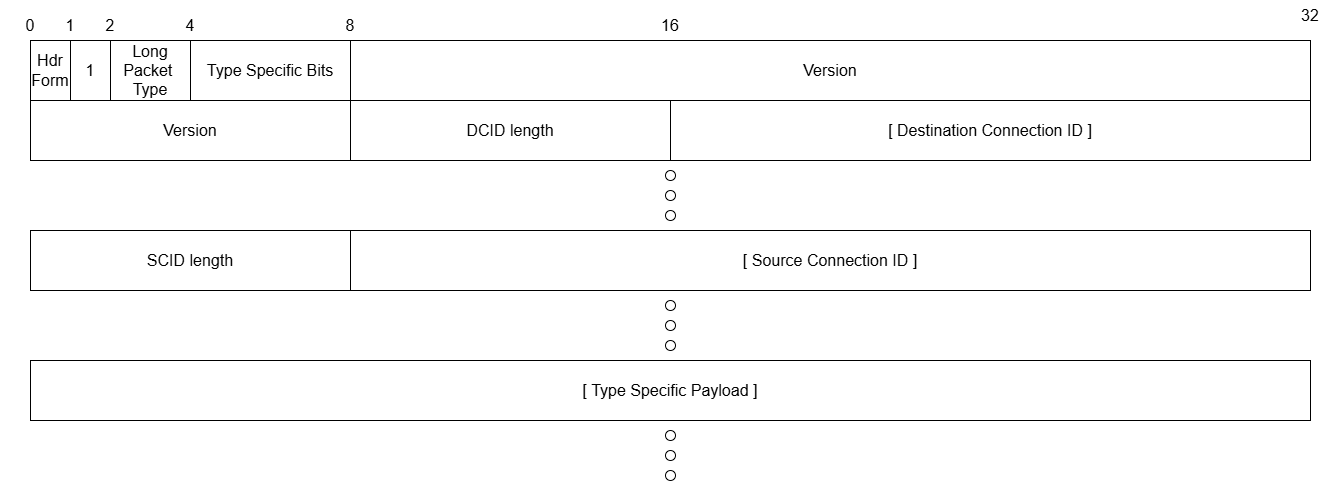
\includegraphics[width=1.0\linewidth]{fig/QUIC/quic_long_header.png}
        \caption{Cabeçalho longo do QUIC.}
        \label{fig:quic_long_header}
\end{figure}

A Figura~\ref{fig:quic_long_header} apresenta o formato do \textit{long header}, utilizado pelos quatro tipos de pacote listados na Tabela~\ref{tab:quic_long_header_packets} e descritos na Seção~\ref{sec:quic_long_header_packets}. O RFC~9000 \citep{rfc9000} define os campos comuns a esses pacotes e os campos específicos de cada tipo, descritos a seguir:


\begin{table}[!ht]
    \centering
    \setstretch{1.3}
    \begin{tabular}{|c|c|}
        \hline
        \textbf{Valor} & \textbf{Tipo de pacote} \\
        \hline
        0x00 & Initial   \\
        0x01 & 0-RTT     \\
        0x02 & Handshake \\
        0x03 & Retry     \\
        \hline
    \end{tabular}
    \caption{Tipos de pacotes QUIC com \textit{long header}. Fonte: \citep{rfc9000}.}
    \label{tab:quic_long_header_packets}
\end{table}

\begin{itemize}
    \item \textbf{Primeiro byte:}
    \begin{itemize}
        \item \textbf{Header Form} (1 bit): identifica o formato do cabeçalho; no \textit{long header}, possui sempre o valor 1;
        \item \textbf{Fixed Bit} (1 bit): possui sempre o valor 1, exceto em pacotes de \textit{Version Negotiation};
        \item \textbf{Long Packet Type} (2 bits): identifica o tipo de pacote, conforme a Tabela~\ref{tab:quic_long_header_packets};
        \item \textbf{Type-Specific Bits} (4 bits): bits cujo significado depende do tipo de pacote. Nos pacotes \texttt{Initial}, \texttt{0-RTT} e \texttt{Handshake}, esses bits contêm dois bits reservados e o campo \textit{Packet Number Length};
    \end{itemize}
    \item \textbf{Version} (32 bits): identifica a versão do QUIC e determina a interpretação dos demais campos; no QUICv1, possui o valor \texttt{0x00000001};
    \item \textbf{Destination Connection ID Length} (8 bits): indica o tamanho, em bytes, do campo seguinte;
    \item \textbf{Destination Connection ID} (DCID, 0 a 160 bits): identificador de conexão escolhido pelo receptor do pacote;
    \item \textbf{Source Connection ID Length} (8 bits): indica o tamanho, em bytes, do campo seguinte;
    \item \textbf{Source Connection ID} (SCID, 0 a 160 bits): identificador de conexão escolhido pelo emissor do pacote;
    \item \textbf{Type-Specific Payload}: campos específicos de cada tipo de pacote, descritos na Seção~\ref{sec:quic_long_header_packets}.
\end{itemize}

\subsubsection{Short Header}
\label{sec:quic_short_header}



A Figura~\ref{fig:quic_short_header} apresenta o formato do \textit{short header}. Diferentemente do \textit{long header}, que transporta informações necessárias apenas ao estabelecimento da conexão, como a versão e os comprimentos dos \textit{Connection IDs}, o \textit{short header} é utilizado na transmissão de dados e de controle ao longo da conexão e, por isso, é mais compacto. Pacotes com \textit{short header} podem ser enviados antes do término do \textit{handshake}, assim que as chaves 1-RTT estão disponíveis; no caso do servidor, isso ocorre logo após o envio de sua mensagem \texttt{Finished}.

\begin{figure}[!ht]
        \centering
        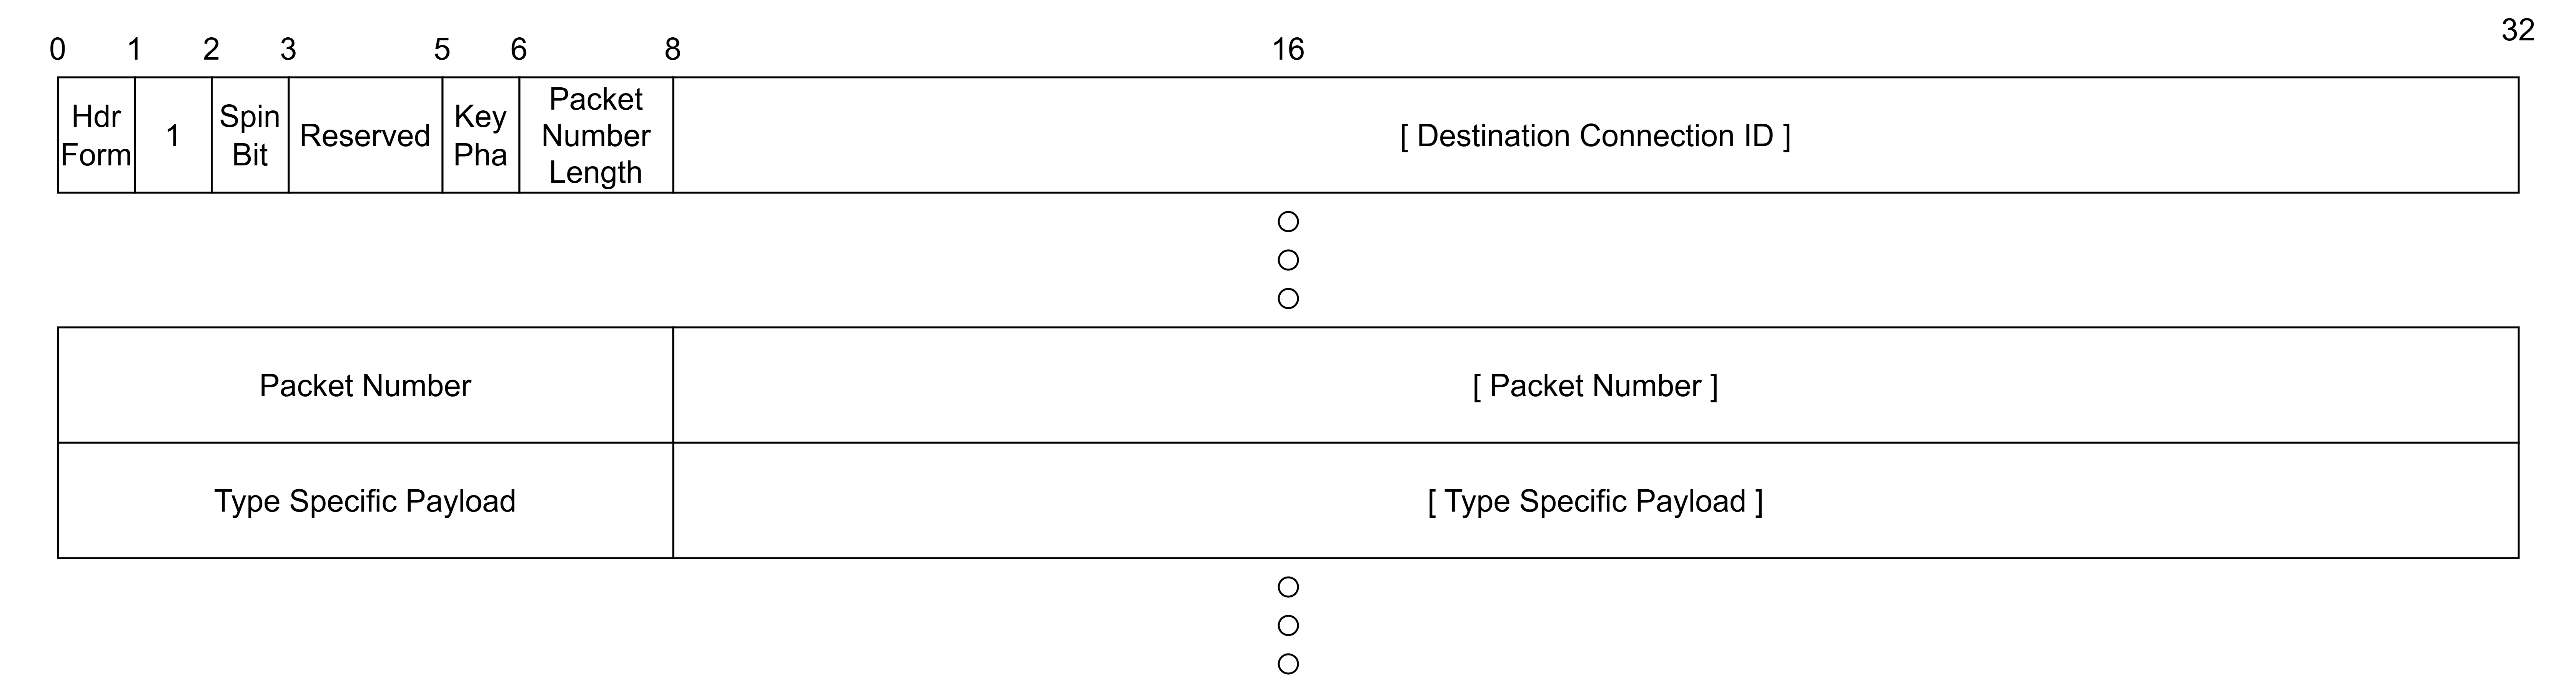
\includegraphics[width=1.0\linewidth]{fig/QUIC/quic_short_header.png}
        \caption{Cabeçalho curto do QUIC.}
        \label{fig:quic_short_header}
\end{figure}


O \textit{short header} possui um único tipo de pacote, o \texttt{1-RTT}, descrito na Seção~\ref{sec:quic_short_header_packets}. O RFC~9000 \citep{rfc9000} define seus campos, descritos a seguir:

\begin{itemize}
    \item \textbf{Primeiro byte:}
    \begin{itemize}
        \item \textbf{Header Form} (1 bit): identifica o formato do cabeçalho; no \textit{short header}, possui sempre o valor 0;
        \item \textbf{Fixed Bit} (1 bit): possui sempre o valor 1;
        \item \textbf{Spin Bit} (1 bit): permite que um observador externo meça o RTT da conexão sem decifrar os pacotes. Ao receber um pacote cujo número é maior que o de todos os pacotes recebidos do outro \textit{endpoint}, o servidor replica o valor do \textit{spin bit} recebido, enquanto o cliente envia o valor invertido. Essa assimetria faz o bit alternar uma vez a cada RTT em cada direção, o que permite ao observador estimar o RTT pela observação dessas alternâncias. Como expõe informação sobre a conexão, o mecanismo pode ser desabilitado por qualquer \textit{endpoint}; nesse caso, o \textit{spin bit} recebe valores aleatórios;
        \item \textbf{Reserved Bits} (2 bits): bits reservados, que devem possuir o valor 0;
        \item \textbf{Key Phase} (1 bit): indica qual geração de chaves protege o pacote. A alternância desse bit sinaliza a atualização de chaves (\textit{key update}), o que permite ao QUIC renovar as chaves de uma conexão sem um novo \textit{handshake};
        \item \textbf{Packet Number Length} (2 bits): indica o tamanho do campo \textit{Packet Number}, em bytes, menos um;
    \end{itemize}
    \item \textbf{Destination Connection ID} (0 a 160 bits): identificador de conexão do destinatário. O cabeçalho não indica o tamanho desse campo, pois o destinatário escolheu o próprio identificador e, portanto, conhece seu tamanho;
    \item \textbf{Packet Number} (8 a 32 bits): número do pacote, codificado de forma truncada com o tamanho indicado pelo campo \textit{Packet Number Length};
    \item \textbf{Packet Payload}: conteúdo cifrado do pacote, composto por um ou mais \textit{frames}.
\end{itemize}

\subsubsection{Proteção de cabeçalho}
\label{sec:quic_header_protection}

Estudos como o de \citep{reed2017identifying} demonstram que os metadados expostos pelo tráfego cifrado podem comprometer a confidencialidade da informação transmitida. Para reduzir esses metadados, o QUIC cifra, além do \textit{payload}, parte do cabeçalho, mecanismo denominado \textit{header protection} \citep{rfc9001}. A proteção abrange o número do pacote e bits do primeiro byte, o que dificulta a correlação de pacotes por observadores externos e impede que \textit{middleboxes} passem a depender desses campos, preservando a capacidade de evolução do protocolo.

Para cada nível de criptografia (\textit{Initial}, \textit{0-RTT}, \textit{Handshake} e \textit{1-RTT}), o QUIC deriva um segredo, a partir do qual a função HKDF (\textit{HMAC-based Key Derivation Function}) gera três valores: a chave de proteção do pacote, um IV (\textit{Initialization Vector}) e a chave de proteção do cabeçalho \citep{rfc9001}. Na proteção do pacote, o \textit{nonce} exigido pelo algoritmo AEAD (\textit{Authenticated Encryption with Associated Data}) resulta do XOR entre o IV e o número completo do pacote, completado com zeros à esquerda até o tamanho do IV. Como os números de pacote não se repetem em um mesmo espaço de numeração, o \textit{nonce} é único para cada pacote cifrado com a mesma chave.

Na proteção do cabeçalho, o número do pacote não pode servir como entrada, pois o receptor precisa remover essa proteção para conhecê-lo. Por isso, o QUIC utiliza como entrada uma amostra de 16 bytes do próprio \textit{ciphertext} do pacote, iniciada 4 bytes após o início do campo \textit{Packet Number}. Por resultar da cifragem, essa amostra é pseudoaleatória e cumpre o papel de um segundo \textit{nonce} \citep{marx2020quic}. A amostra e a chave de proteção do cabeçalho alimentam uma função que gera uma máscara: o AES em modo ECB (\textit{Electronic Code Book}), quando a suíte de cifras utiliza AES, ou o ChaCha20, quando a suíte utiliza ChaCha20-Poly1305 \citep{rfc9001}. A máscara é combinada via XOR com os bits menos significativos do primeiro byte, quatro no \textit{long header} e cinco no \textit{short header}, e com os bytes do campo \textit{Packet Number}.

A Figura~\ref{fig:quic_short_header_protection} ilustra a aplicação da \textit{header protection} a um pacote com \textit{short header}.

\begin{figure}[ht]
    \centering
    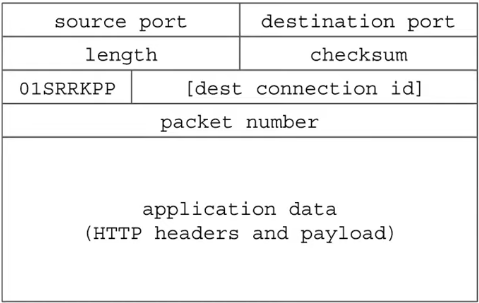
\includegraphics[width=0.45\textwidth]{fig/QUIC/quic_header.png}
    \hfill
    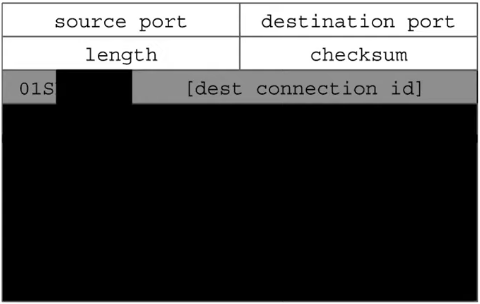
\includegraphics[width=0.45\textwidth]{fig/QUIC/quic_header_enc.png}
    \caption{\textit{Header protection} do QUIC em pacotes \textit{short header}. Fonte: adaptado de \citep{marx2020quic}.}
    \label{fig:quic_short_header_protection}
\end{figure}

\subsection{Tipos de pacotes QUIC}

O QUIC define seis tipos de pacote: \texttt{Initial}, \texttt{0-RTT}, \texttt{Handshake} e \texttt{Retry}, com \textit{long header}; \texttt{1-RTT}, com \textit{short header}; e \textit{Version Negotiation}, descrito na Seção~\ref{sec:version_negotiation_packet}. Os pacotes \texttt{Initial}, \texttt{0-RTT}, \texttt{Handshake} e \texttt{1-RTT} estão associados a um nível de criptografia, discutido na Seção~\ref{sec:quic_packet_protection}, e a um dos três espaços de números de pacote (\textit{packet number spaces}): \textit{Initial}, \textit{Handshake} e \textit{Application Data}, este último compartilhado pelos pacotes \texttt{0-RTT} e \texttt{1-RTT}. Cada espaço mantém sua própria numeração, independente dos demais, conforme discutido na Seção~\ref{sec:quic_acknowledgement}. Os pacotes \texttt{Retry} e \textit{Version Negotiation} não possuem número de pacote; o \texttt{Retry} possui apenas uma etiqueta de integridade, e o \textit{Version Negotiation} não possui proteção criptográfica.

\subsubsection{Pacotes com \textit{long header}}
\label{sec:quic_long_header_packets}

Os pacotes com \textit{long header} são utilizados durante o estabelecimento da conexão, até que os \textit{endpoints} passem a utilizar as chaves 1-RTT. Esses pacotes utilizam o cabeçalho descrito na Seção~\ref{sec:quic_long_header}, e seus tipos estão listados na Tabela~\ref{tab:quic_long_header_packets}.


\paragraph{Pacote Initial}

O pacote \texttt{Initial} transporta as primeiras mensagens do \textit{handshake} TLS, o \texttt{Client Hello} e o \texttt{ServerHello}, em \textit{frames} \texttt{CRYPTO}. Suas chaves derivam do DCID escolhido pelo cliente e de um \textit{salt} fixo definido pela versão do protocolo \citep{rfc9001}; como esses valores são públicos, qualquer observador pode decifrar os pacotes \texttt{Initial}. Essa proteção, portanto, não oferece confidencialidade, mas dificulta a injeção de pacotes por atacantes fora do caminho da conexão (\textit{off-path}). O cabeçalho do pacote \texttt{Initial} inclui ainda um campo \textit{Token}, utilizado na validação de endereço, e os datagramas que transportam pacotes \texttt{Initial} do cliente devem ter ao menos 1200 bytes. A Tabela~\ref{tab:quic_frames_tab} apresenta os demais \textit{frames} permitidos nesse pacote.

\paragraph{Pacote 0-RTT}

O pacote \texttt{0-RTT} transporta dados de aplicação enviados pelo cliente na primeira transmissão de mensagens, junto ao pacote \texttt{Initial}, antes da conclusão do \textit{handshake}. Esse pacote só pode ser utilizado na retomada de uma sessão anterior: suas chaves derivam de uma PSK (\textit{Pre-Shared Key}) obtida pelo cliente na conexão anterior, por meio de um \textit{session ticket} do TLS~1.3 \citep{rfc8446}. Os dados 0-RTT são cifrados, mas não possuem sigilo futuro (\textit{forward secrecy}) e podem ser reproduzidos por um atacante (\textit{replay}), de modo que a aplicação deve restringir seu uso a operações idempotentes. A Seção~\ref{sec:0rtt_connection_recovery} descreve o uso desses pacotes na retomada de sessão.

\paragraph{Pacote Handshake}

O pacote \texttt{Handshake} transporta, em \textit{frames} \texttt{CRYPTO}, as mensagens do \textit{handshake} TLS posteriores ao \texttt{ServerHello}: \texttt{EncryptedExtensions}, \texttt{Certificate}, \texttt{CertificateVerify} e \texttt{Finished} do servidor e a mensagem \texttt{Finished} do cliente. Esses pacotes são protegidos pelas \textit{Handshake keys}, derivadas do segredo compartilhado obtido na troca de chaves (EC)DHE (\textit{(Elliptic Curve) Diffie-Hellman Ephemeral}) realizada por meio do \texttt{ClientHello} e do \texttt{ServerHello}. Diferentemente das chaves \textit{Initial}, as \textit{Handshake keys} oferecem confidencialidade, pois dependem de um segredo conhecido apenas pelos \textit{endpoints}. A Tabela~\ref{tab:quic_frames_tab} apresenta os demais \textit{frames} permitidos nesse pacote.

\paragraph{Pacote Retry}

O pacote \texttt{Retry} é enviado pelo servidor em resposta a um pacote \texttt{Initial} do cliente, com o objetivo de validar o endereço deste antes de alocar recursos para a conexão. O pacote transporta um \textit{Retry Token}, que o cliente deve repetir no campo \textit{Token} de um novo pacote \texttt{Initial}. Ao receber o \textit{token}, o servidor confirma que o cliente recebe pacotes no endereço declarado, o que dificulta ataques com endereço de origem forjado (\textit{spoofing}). A Seção~\ref{sec:quic_connection} discute a validação de endereço. O pacote \texttt{Retry} não transporta \textit{frames} nem é cifrado, mas inclui uma \textit{Retry Integrity Tag}, calculada com uma chave fixa definida pelo RFC~9001 sobre o conteúdo do pacote e o DCID original do cliente \citep{rfc9001}. Como a chave é pública, a etiqueta não oferece autenticação, mas permite descartar pacotes corrompidos pela rede e garante que apenas uma entidade que observou o pacote \texttt{Initial} original consiga gerar um \texttt{Retry} válido.

\subsubsection{Pacote de \textit{Version Negotiation}}
\label{sec:version_negotiation_packet}

O pacote de \textit{Version Negotiation} utiliza o formato de \textit{long header} e é enviado pelo servidor em resposta a um pacote do cliente cuja versão o servidor não suporta. O pacote lista as versões aceitas pelo servidor e repete os \textit{Connection IDs} do pacote recebido, com os campos de origem e destino invertidos, o que permite ao cliente verificar que a resposta corresponde ao pacote que enviou.

Como esse pacote independe de versão, seu formato é definido pelo RFC~8999 \citep{rfc8999}, que admite \textit{Connection IDs} de até 255 bytes. O limite de 20 bytes aplica-se apenas aos pacotes do QUICv1 \citep{rfc9000}: um \textit{endpoint} descarta pacotes da versão 1 com \textit{Connection IDs} maiores, mas um servidor deve ser capaz de ler identificadores mais longos de outras versões para formar corretamente o pacote de \textit{Version Negotiation}.

\begin{figure}[!ht]
        \centering
        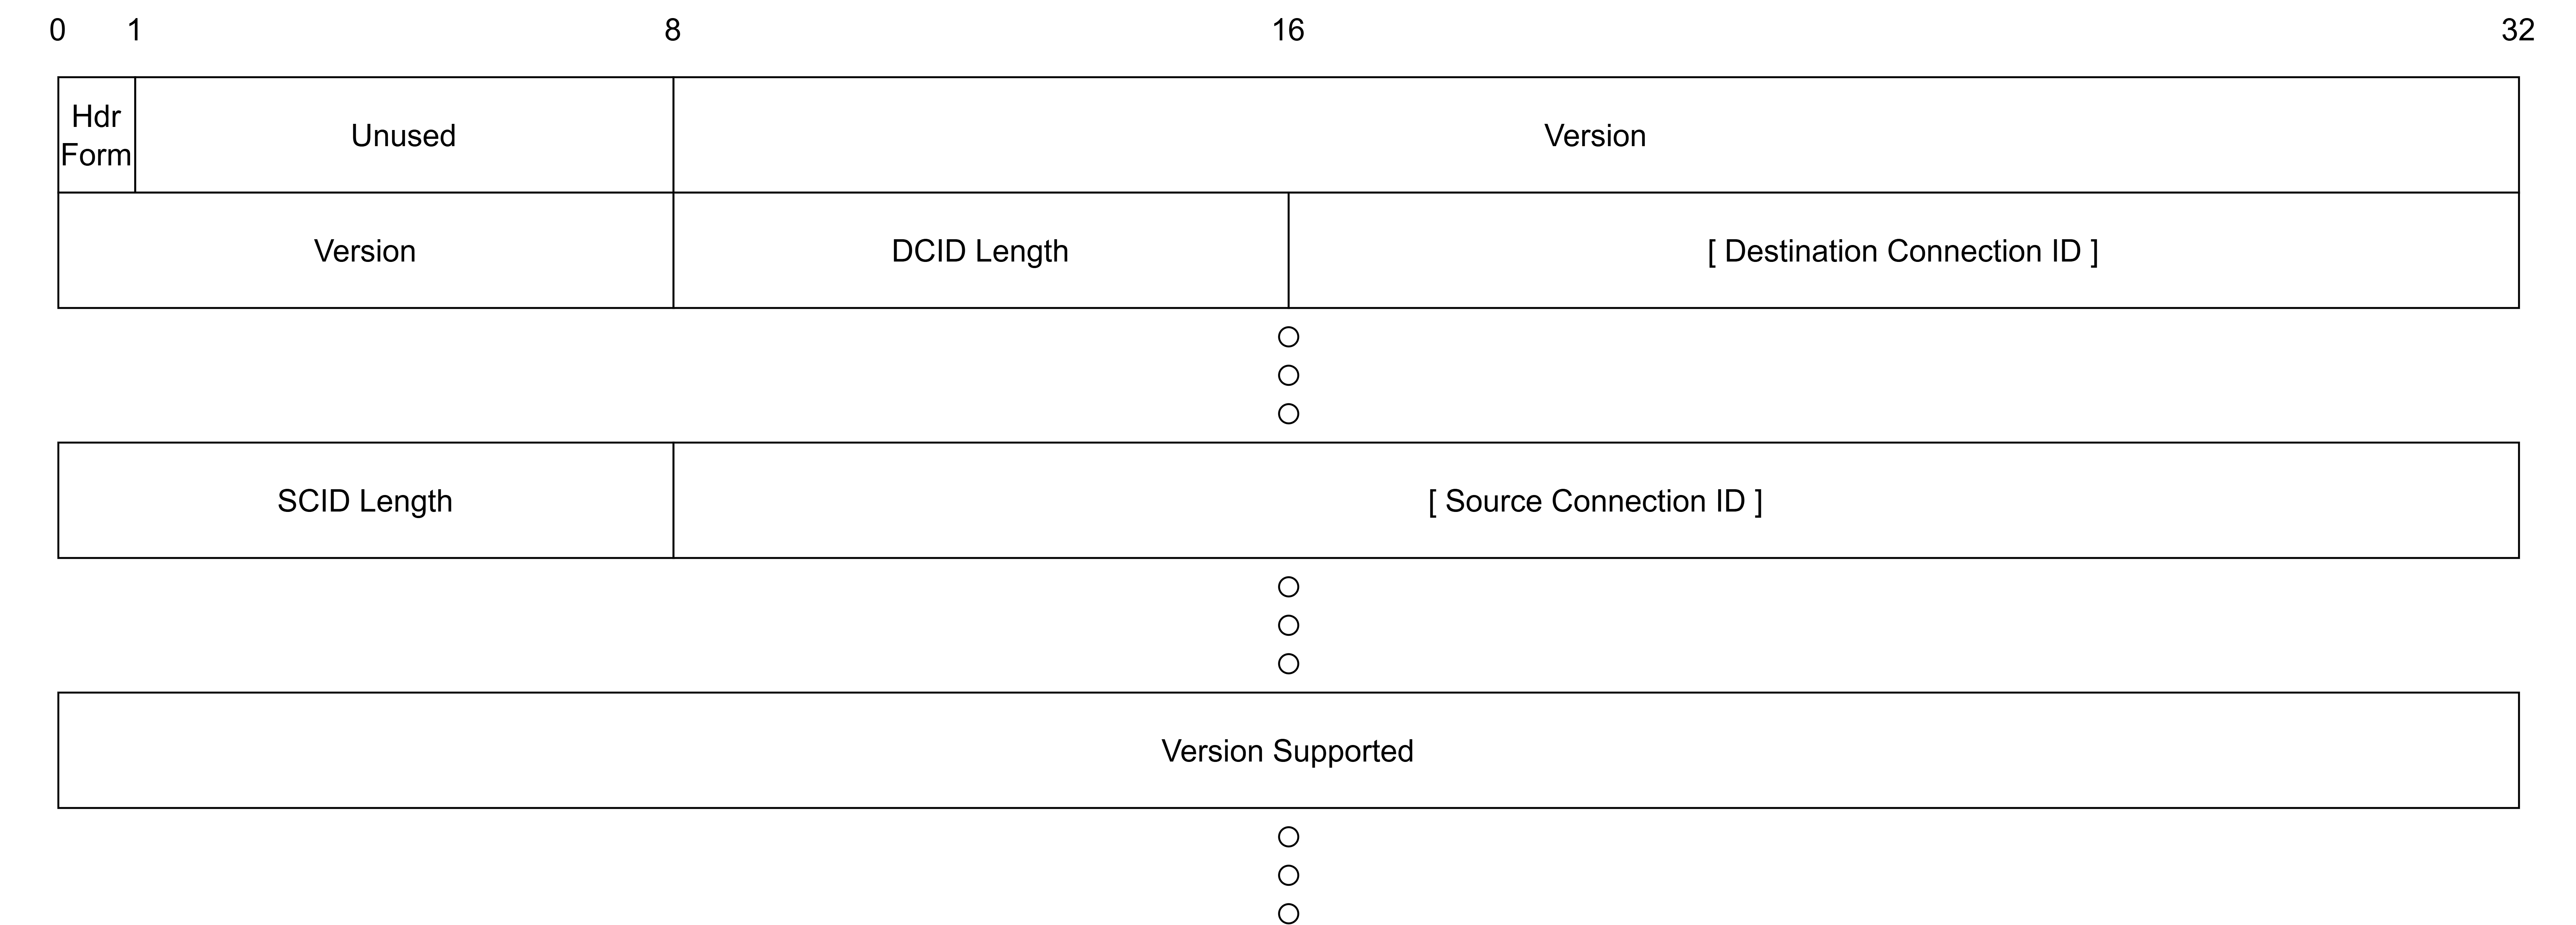
\includegraphics[width=1.0\linewidth]{fig/QUIC/quic_version_negotiation_packet.png}
        \caption{Pacote de Version Negotiation do QUIC.}
        \label{fig:quic_version_negotiation_packet}
\end{figure}

A Figura~\ref{fig:quic_version_negotiation_packet} apresenta o formato do pacote, cujos campos são descritos a seguir:

\begin{itemize}
    \item \textbf{Primeiro byte:}
    \begin{itemize}
        \item \textbf{Header Form} (1 bit): possui o valor 1, como no \textit{long header};
        \item \textbf{Unused} (7 bits): bits com valor arbitrário definido pelo servidor e ignorados pelo cliente. Quando o QUIC compartilha a porta com outros protocolos, o servidor deve atribuir o valor 1 ao bit mais significativo desse campo;
    \end{itemize}
    \item \textbf{Version} (32 bits): possui o valor \texttt{0x00000000}, reservado para identificar o pacote de \textit{Version Negotiation} e que nenhuma versão do protocolo pode utilizar;
    \item \textbf{Destination Connection ID Length} (8 bits) e \textbf{Destination Connection ID} (0 a 255 bytes): repetem o SCID do pacote recebido do cliente;
    \item \textbf{Source Connection ID Length} (8 bits) e \textbf{Source Connection ID} (0 a 255 bytes): repetem o DCID do pacote recebido do cliente;
    \item \textbf{Supported Version} (32 bits cada): lista das versões suportadas pelo servidor.
\end{itemize}

\subsubsection{Pacotes com \textit{short header}}
\label{sec:quic_short_header_packets}

Os pacotes com \textit{short header} transportam dados e informações de controle após o estabelecimento das chaves 1-RTT, conforme descrito na Seção~\ref{sec:quic_short_header}. No QUICv1, o \textit{short header} possui um único tipo de pacote, o \texttt{1-RTT}.

\paragraph{Pacote 1-RTT}

O pacote \texttt{1-RTT} pode transportar a maioria dos tipos de \textit{frame}, conforme a Tabela~\ref{tab:quic_frames_tab}, e é utilizado principalmente após a conclusão do \textit{handshake}. O servidor, entretanto, dispõe das chaves 1-RTT logo após enviar sua mensagem \texttt{Finished}, antes de receber a mensagem \texttt{Finished} do cliente, e pode enviar dados de aplicação nesse intervalo. Esses dados são denominados 0.5-RTT \citep{rfc9001}. Como o servidor ainda não verificou o \texttt{Finished} do cliente, os dados 0.5-RTT não devem depender da autenticação do cliente. Após a conclusão do \textit{handshake}, ambos os \textit{endpoints} utilizam as chaves 1-RTT.

\subsubsection{Proteção de pacotes}
\label{sec:quic_packet_protection}

Esta seção detalha a proteção aplicada aos pacotes QUIC em cada nível de criptografia, que complementa a proteção de cabeçalho descrita na Seção~\ref{sec:quic_header_protection}. Com exceção do \textit{Version Negotiation}, todos os tipos de pacote possuem algum mecanismo de proteção, descrito a seguir.

\paragraph{Initial Secrets}

Os \textit{Initial Secrets} são os segredos utilizados na proteção dos pacotes \texttt{Initial}. O QUIC calcula um segredo inicial pela função HKDF-Extract, a partir de um \textit{salt} fixo definido para a versão e do DCID escolhido pelo cliente em seu primeiro pacote \texttt{Initial} \citep{rfc9001}. Desse segredo derivam dois segredos distintos, um para cada sentido da comunicação, obtidos com os rótulos \texttt{client in} e \texttt{server in}. Se o servidor responder com um pacote \texttt{Retry}, o cliente recalcula os segredos com o novo DCID, escolhido pelo servidor no campo SCID do \texttt{Retry}.

\paragraph{0-RTT Keys}

As chaves 0-RTT derivam da PSK obtida em uma sessão anterior com o mesmo servidor e, portanto, são distintas das chaves 1-RTT, que dependem também do segredo (EC)DHE negociado na conexão atual. Como dependem apenas da PSK, as chaves 0-RTT não oferecem \textit{forward secrecy}: o comprometimento da PSK expõe os dados 0-RTT de todas as conexões que a utilizaram. Além disso, um atacante pode reenviar pacotes 0-RTT capturados (\textit{replay}), fazendo com que o servidor processe a mesma requisição mais de uma vez. Por isso, o RFC~9001 \citep{rfc9001} exige que o protocolo de aplicação defina quais operações podem ser enviadas em 0-RTT, em geral apenas as idempotentes. Os pacotes 0-RTT aceitam apenas parte dos tipos de \textit{frame}, conforme a Tabela~\ref{tab:quic_frames_tab}, e o cliente pode enviá-los até obter as chaves 1-RTT.

\paragraph{Handshake Keys}

As \textit{Handshake Keys} derivam do \textit{Handshake Secret} do TLS~1.3, obtido a partir do segredo compartilhado da troca de chaves (EC)DHE \citep{rfc8446}. Desse segredo, o TLS deriva um segredo de tráfego para cada sentido, com os rótulos \texttt{c hs traffic} e \texttt{s hs traffic}, que incorporam o \textit{hash} das mensagens \texttt{ClientHello} e \texttt{ServerHello}. A esses segredos, o QUIC aplica os rótulos \texttt{quic key}, \texttt{quic iv} e \texttt{quic hp} para obter as chaves de proteção do pacote, o IV e a chave de proteção do cabeçalho \citep{rfc9001}. Essas chaves protegem apenas os pacotes \texttt{Handshake}.

\paragraph{Retry Integrity Tag}
\label{sec:quic_retry_integrity_tag}

A \textit{Retry Integrity Tag} é um campo de 128 bits que encerra o pacote \texttt{Retry}. O servidor a calcula com o algoritmo AEAD\_AES\_128\_GCM, que utiliza uma chave e um \textit{nonce} fixos definidos pelo RFC~9001 \citep{rfc9001}, um texto claro vazio e, como dados associados, um pseudopacote formado pelo DCID original do cliente e pelo conteúdo do \texttt{Retry}. Como a chave é pública, a etiqueta não envolve derivação de chaves nem oferece confidencialidade ou autenticação, mas protege o pacote contra corrupção acidental e contra atacantes que não observaram o pacote \texttt{Initial} original.

\paragraph{1-RTT Keys}

As \textit{1-RTT Keys} derivam do \textit{Master Secret} do TLS~1.3, que, por sua vez, deriva do \textit{Handshake Secret} \citep{rfc8446}. Do \textit{Master Secret}, o TLS obtém um segredo de tráfego de aplicação para cada sentido, com os rótulos \texttt{c ap traffic} e \texttt{s ap traffic}, que incorporam o \textit{hash} das mensagens do \textit{handshake} até o \texttt{Finished} do servidor. Assim como nas \textit{Handshake Keys}, o QUIC aplica a esses segredos os rótulos \texttt{quic key}, \texttt{quic iv} e \texttt{quic hp} \citep{rfc9001}. Na atualização de chaves sinalizada pelo bit \textit{Key Phase}, o QUIC deriva um novo segredo com o rótulo \texttt{quic ku}, sem alterar a chave de proteção do cabeçalho. As \textit{1-RTT Keys} protegem exclusivamente os pacotes \texttt{1-RTT}.

\subsubsection{\textit{Frames} do QUIC}

Com exceção dos pacotes \texttt{Retry} e \textit{Version Negotiation}, o \textit{payload} de um pacote QUIC é composto por uma sequência de \textit{frames}. Cada tipo de pacote admite apenas determinados tipos de \textit{frame}, conforme a Tabela~\ref{tab:quic_frames_tab}. A função de cada tipo de \textit{frame} é definida no RFC~9000 \citep{rfc9000} e não é detalhada neste trabalho.


\begin{table}[!ht]
\centering
\begin{tabular}{|c|l|l|}
\hline
\textbf{Valor} & \textbf{Tipo de \textit{frame}} & \textbf{Pacotes} \\ \hline
0x00       & PADDING                 & Initial, 0-RTT, Handshake, 1-RTT \\ \hline
0x01       & PING                    & Initial, 0-RTT, Handshake, 1-RTT \\ \hline
0x02--0x03 & ACK                     & Initial, Handshake, 1-RTT \\ \hline
0x04       & RESET\_STREAM            & 0-RTT, 1-RTT \\ \hline
0x05       & STOP\_SENDING            & 0-RTT, 1-RTT \\ \hline
0x06       & CRYPTO                  & Initial, Handshake, 1-RTT \\ \hline
0x07       & NEW\_TOKEN               & 1-RTT \\ \hline
0x08--0x0f & STREAM                  & 0-RTT, 1-RTT \\ \hline
0x10       & MAX\_DATA                & 0-RTT, 1-RTT \\ \hline
0x11       & MAX\_STREAM\_DATA        & 0-RTT, 1-RTT \\ \hline
0x12--0x13 & MAX\_STREAMS             & 0-RTT, 1-RTT \\ \hline
0x14       & DATA\_BLOCKED            & 0-RTT, 1-RTT \\ \hline
0x15       & STREAM\_DATA\_BLOCKED    & 0-RTT, 1-RTT \\ \hline
0x16--0x17 & STREAMS\_BLOCKED         & 0-RTT, 1-RTT \\ \hline
0x18       & NEW\_CONNECTION\_ID      & 0-RTT, 1-RTT \\ \hline
0x19       & RETIRE\_CONNECTION\_ID   & 1-RTT \\ \hline
0x1a       & PATH\_CHALLENGE          & 0-RTT, 1-RTT \\ \hline
0x1b       & PATH\_RESPONSE           & 1-RTT \\ \hline
0x1c       & CONNECTION\_CLOSE        & Initial, 0-RTT, Handshake, 1-RTT \\ \hline
0x1d       & CONNECTION\_CLOSE        & 0-RTT, 1-RTT \\ \hline
0x1e       & HANDSHAKE\_DONE          & 1-RTT \\ \hline
\end{tabular}
\caption{Tipos de \textit{frame} do QUIC e pacotes que podem transportá-los. Fonte: adaptado de \citep{rfc9000}.}
\label{tab:quic_frames_tab}
\end{table}


\section{Conexão do QUIC}
\label{sec:quic_connection}

O estabelecimento de conexão do QUIC segue diferentes fluxos, conforme o estado prévio dos \textit{endpoints} e os pacotes recebidos. Esta seção descreve o \textit{handshake} 1-RTT, utilizado como caso base, e suas variações:

\begin{itemize}
    \item A Seção~\ref{sec:quic_connection_steps} detalha as etapas do \textit{handshake} 1-RTT do QUICv1;
    \item A Seção~\ref{sec:0rtt_connection_recovery} descreve a retomada de sessão com dados 0-RTT;
    \item A Seção~\ref{sec:quic_version_negotiation} descreve a negociação da versão do protocolo entre os \textit{endpoints};
    \item A Seção~\ref{sec:quic_address_validation} descreve a validação de endereço, que mitiga ataques de \textit{spoofing} e de amplificação;
    \item A Seção~\ref{sec:connection_ids_operation} descreve o funcionamento dos \textit{Connection IDs}.
\end{itemize}

A Seção~\ref{sec:quic_connection_steps} descreve o \textit{handshake} TLS apenas no nível necessário à compreensão do QUIC; o funcionamento detalhado do TLS~1.3 é definido no RFC~8446 \citep{rfc8446}.

\subsection{Etapas de conexão do QUIC}
\label{sec:quic_connection_steps}

No fluxo padrão, denominado \textit{handshake} 1-RTT, o QUIC combina o estabelecimento da conexão de transporte com o \textit{handshake} TLS~1.3: os parâmetros de transporte de cada \textit{endpoint} são trocados em uma extensão do próprio TLS \citep{rfc9001}. Assim, o cliente pode enviar dados de aplicação após um único RTT, enquanto a combinação de TCP e TLS~1.3 exige dois RTTs: um para o \textit{3-way handshake} do TCP e outro para o \textit{handshake} TLS. A Figura~\ref{fig:quic_vs_tcptls} compara os dois fluxos.

\begin{figure}[!ht]
        \centering
        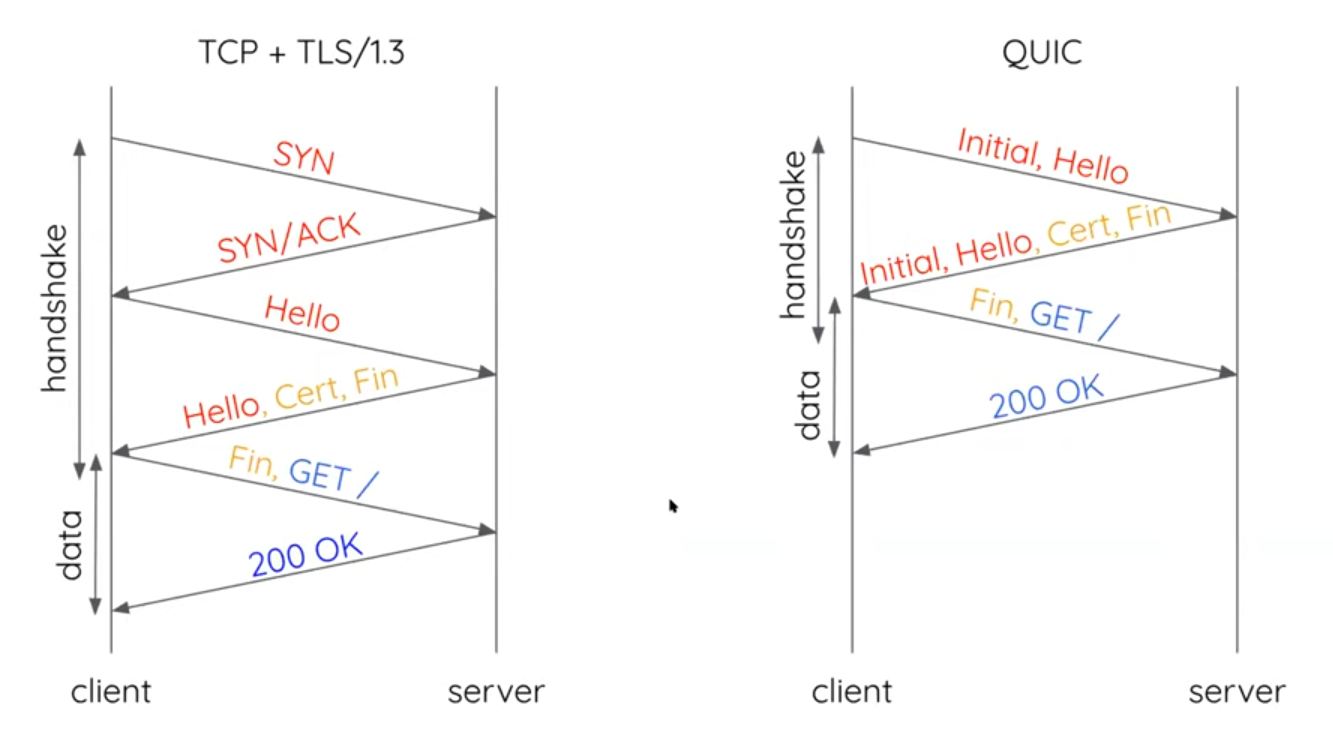
\includegraphics[width=0.85\linewidth]{fig/QUIC/quic_vs_tcptls_cmp.png}
        \caption{Comparação entre conexões do TCP/TLS e QUIC. Fonte: adaptado de \citep{marx2020quic}.}
        \label{fig:quic_vs_tcptls}
\end{figure}

O \textit{handshake} 1-RTT ocorre da seguinte forma. O cliente envia um pacote \texttt{Initial} com a mensagem \texttt{ClientHello}, que contém sua parcela da troca de chaves (EC)DHE e seus parâmetros de transporte.

O servidor responde com um pacote \texttt{Initial}, que contém a confirmação de recebimento (\textit{frame} \texttt{ACK}) do pacote do cliente e a mensagem \texttt{ServerHello}, e com um pacote \texttt{Handshake}, que contém as mensagens \texttt{EncryptedExtensions}, \texttt{Certificate}, \texttt{CertificateVerify} e \texttt{Finished}. Opcionalmente, o servidor envia também um pacote \texttt{1-RTT} com dados 0.5-RTT, discutidos na Seção~\ref{sec:quic_short_header_packets}. Esses pacotes podem ser agrupados em um mesmo datagrama UDP (\textit{coalescing}).

O cliente confirma o recebimento dos pacotes \texttt{Initial} e \texttt{Handshake} do servidor e conclui sua parte do \textit{handshake} TLS ao enviar a mensagem \texttt{Finished} em um pacote \texttt{Handshake}. A partir desse momento, o cliente pode enviar dados de aplicação em pacotes \texttt{1-RTT}.

Ao receber o \texttt{Finished} do cliente, o servidor considera o \textit{handshake} concluído e confirmado e envia ao cliente um \textit{frame} \texttt{HANDSHAKE\_\allowbreak{}DONE}. O cliente, por sua vez, considera o \textit{handshake} confirmado ao receber esse \textit{frame}. A confirmação permite que os \textit{endpoints} descartem as chaves de \textit{Handshake} e é pré-requisito para operações como a migração de conexão, discutida na Seção~\ref{sec:quic_connection_migration}. A Figura~\ref{fig:quic_connection_steps_time_diagram} ilustra esse fluxo.

\begin{figure}[!ht]
        \centering
        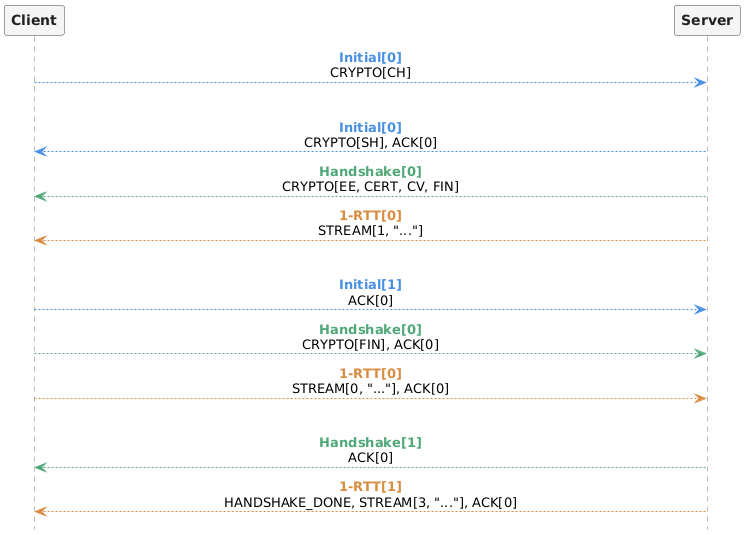
\includegraphics[width=0.9\linewidth]{fig/QUIC/quic_connection_steps.png}
        \caption{Diagrama de tempo do \textit{handshake} 1-RTT do QUIC. Fonte: elaborado com base em \citep{rfc9000}.}
        \label{fig:quic_connection_steps_time_diagram}
\end{figure}

\subsection{Retomada de sessão (0-RTT)}
\label{sec:0rtt_connection_recovery}


A retomada de sessão permite que o cliente reaproveite o estado criptográfico de uma conexão anterior com o mesmo servidor. Nessa conexão anterior, o servidor envia ao cliente um \textit{session ticket} do TLS~1.3, a partir do qual o cliente obtém uma PSK. Em uma nova conexão, o cliente deriva dessa PSK as chaves 0-RTT e envia dados de aplicação, em \textit{frames} \texttt{STREAM}, no primeiro voo de mensagens, junto ao pacote \texttt{Initial}, sem aguardar nenhum RTT. O restante do \textit{handshake} segue o fluxo 1-RTT. A Figura~\ref{fig:quic0rtt_vs_tcptls} compara a retomada de sessão no QUIC e no TCP com TLS, e a Figura~\ref{fig:quic_connection_resumption_time_diagram} ilustra o fluxo de pacotes.

\begin{figure}[!ht]
        \centering
        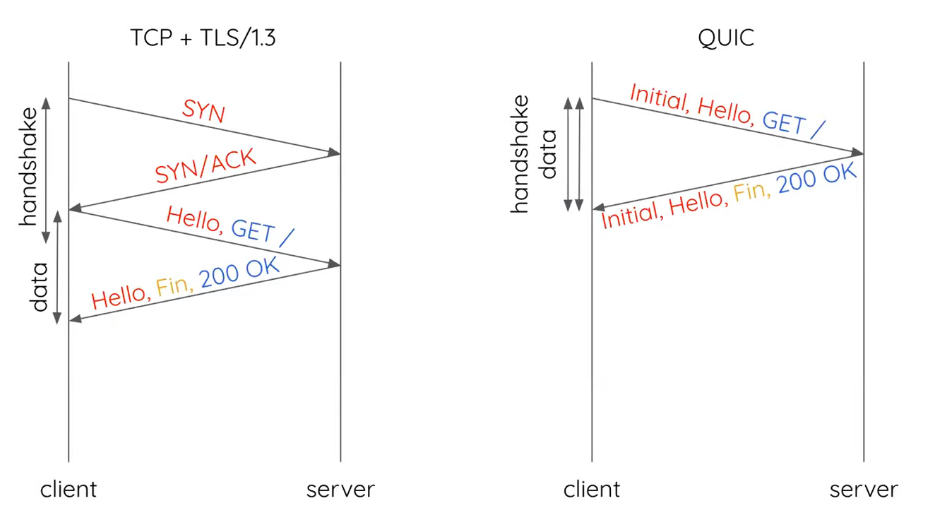
\includegraphics[width=0.8\linewidth]{fig/QUIC/quic0rtt_vs_tcptls_cmp.png}
        \caption{Comparação da retomada de sessão no QUIC (0-RTT) e no TCP com TLS. Fonte: adaptado de \citep{marx2020quic}.}
        \label{fig:quic0rtt_vs_tcptls}
\end{figure}

\begin{figure}[!ht]
        \centering
        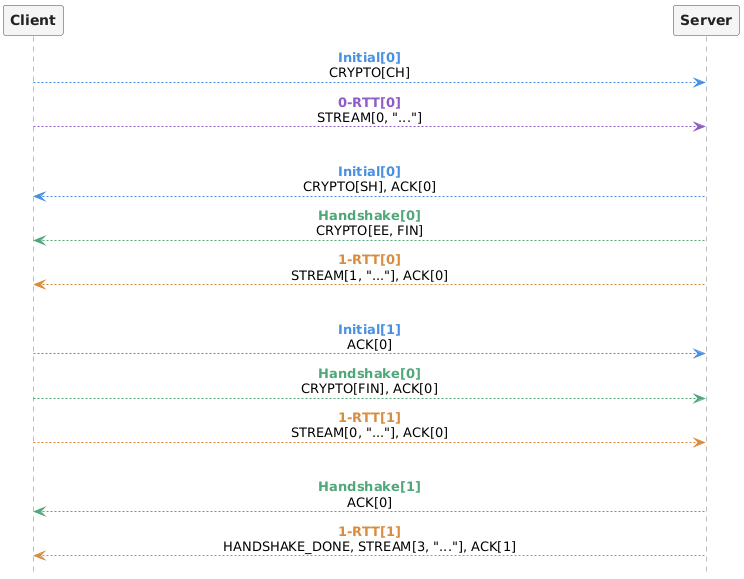
\includegraphics[width=0.7\linewidth]{fig/QUIC/quic_connection_resumption.png}
        \caption{Diagrama de tempo da retomada de sessão do QUIC. Fonte: elaborado com base em \citep{rfc9000}.}
        \label{fig:quic_connection_resumption_time_diagram}
\end{figure}


Os dados 0-RTT, entretanto, estão sujeitos a ataques de \textit{replay}, mencionados na Seção~\ref{sec:quic_packet_protection}: um atacante pode capturar um pacote 0-RTT e reenviá-lo ao servidor, que não consegue distinguir a repetição de uma nova requisição, pois o pacote permanece criptograficamente válido. O critério para decidir o que pode ser enviado em 0-RTT é a idempotência. Operações cuja repetição produz o mesmo efeito de uma única execução, como a leitura de dados, podem ser processadas mais de uma vez sem prejuízo, enquanto operações não idempotentes, como uma compra ou uma transferência financeira, podem ter seus efeitos duplicados. Por isso, protocolos de aplicação como o HTTP/3 definem mecanismos próprios de proteção: o servidor pode responder a uma requisição recebida em 0-RTT com o código de status \texttt{425 Too Early} \citep{rfc8470}, o que leva o cliente a repeti-la após a conclusão do \textit{handshake}.

\subsection{Negociação de versão}
\label{sec:quic_version_negotiation}

A negociação de versão permite que cliente e servidor estabeleçam uma versão comum do QUIC. Ao receber do cliente um pacote com uma versão que não suporta, o servidor responde com um pacote de \textit{Version Negotiation}, que lista as versões aceitas. O cliente então seleciona uma dessas versões e inicia uma nova tentativa de conexão com um novo pacote \texttt{Initial}, o que acrescenta um RTT ao estabelecimento da conexão, conforme a Figura~\ref{fig:quic_version_negotiation_time_diagram}. O servidor não mantém estado durante esse processo e pode limitar o número de pacotes de \textit{Version Negotiation} que envia \citep{rfc9000}. Como esse pacote não é autenticado, o QUICv1 não protege a escolha de versão contra ataques de \textit{downgrade}; o RFC~9368 \citep{rfc9368} define um mecanismo complementar para essa proteção.

\begin{figure}[!ht]
        \centering
        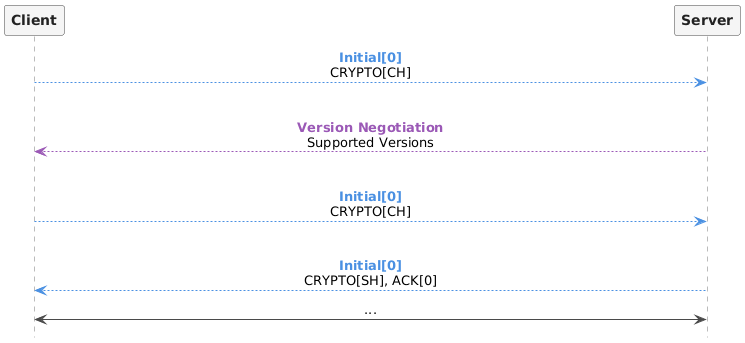
\includegraphics[width=0.7\linewidth]{fig/QUIC/quic_version_negotiation.png}
        \caption{Diagrama de tempo da negociação de versão do QUICv1. Fonte: elaborado com base em \citep{rfc9000}.}
        \label{fig:quic_version_negotiation_time_diagram}
\end{figure}

\subsection{Validação de endereço}
\label{sec:quic_address_validation}

A validação de endereço permite ao servidor confirmar que o cliente recebe pacotes no endereço de origem declarado \citep{rfc9000}. O mecanismo impede que o servidor seja utilizado em ataques de amplificação, nos quais o atacante forja o endereço de origem dos pacotes com o endereço da vítima (\textit{spoofing}), de modo que o servidor envie à vítima um volume de tráfego superior ao gerado pelo atacante. Para isso, o servidor limita os dados enviados a endereços ainda não validados ou valida o endereço antes de prosseguir com o \textit{handshake}. A validação não oferece garantias sobre o conteúdo transmitido; ela apenas confirma que o cliente recebe as respostas no endereço declarado.

Antes da validação, o servidor não pode enviar a um endereço mais do que o triplo dos bytes recebidos desse endereço \citep{rfc9000}. Esse limite de amplificação restringe o tráfego que um atacante consegue direcionar a uma vítima por meio do servidor.

Esse limite pode causar um impasse (\textit{deadlock}): se o servidor o atingir antes de concluir o envio de suas mensagens de \textit{handshake} e as confirmações do cliente se perderem, nenhum dos \textit{endpoints} envia novos pacotes. Para evitar essa situação, o cliente envia pacotes de sondagem (\textit{probe packets}) sempre que seu temporizador de PTO (\textit{Probe Timeout}) expira, mesmo sem dados a transmitir, até ter a garantia de que o servidor validou seu endereço \citep{rfc9002}. Cada pacote recebido amplia a margem de envio do servidor.

Para que o servidor disponha de margem suficiente desde a primeira troca, os datagramas UDP que transportam pacotes \texttt{Initial} do cliente devem ter ao menos 1200 bytes, completados com \textit{frames} \texttt{PADDING} quando necessário. Assim, o servidor pode responder com até 3600 bytes antes de validar o endereço do cliente.

Algumas formas de validação decorrem do próprio \textit{handshake}. O servidor considera validado o endereço do cliente ao receber dele um pacote \texttt{Handshake}, pois o cliente só consegue gerar esse pacote após processar o pacote \texttt{Initial} do servidor. O servidor também pode considerar o endereço validado quando o cliente utiliza um \textit{Connection ID} escolhido pelo servidor com ao menos 64 bits de entropia, já que o cliente só conhece esse identificador se recebeu os pacotes do servidor.

Quando o servidor deseja validar o endereço do cliente antes de prosseguir com o \textit{handshake}, ele responde ao primeiro pacote \texttt{Initial} com um pacote \texttt{Retry} que contém um \textit{token} \citep{rfc9000}. O cliente deve repetir esse \textit{token} no campo \textit{Token} de seu novo pacote \texttt{Initial}, o que comprova o recebimento do \texttt{Retry} no endereço declarado. Como apenas o servidor que emitiu o \textit{token} o valida, seu formato não é padronizado; o servidor deve apenas impedir que outra entidade o forje, em geral por meio de autenticação criptográfica que vincula o \textit{token} ao endereço do cliente. Esse mecanismo acrescenta um RTT ao estabelecimento da conexão, conforme a Figura~\ref{fig:quic_retry_with_token}.

\begin{figure}[!ht]
        \centering
        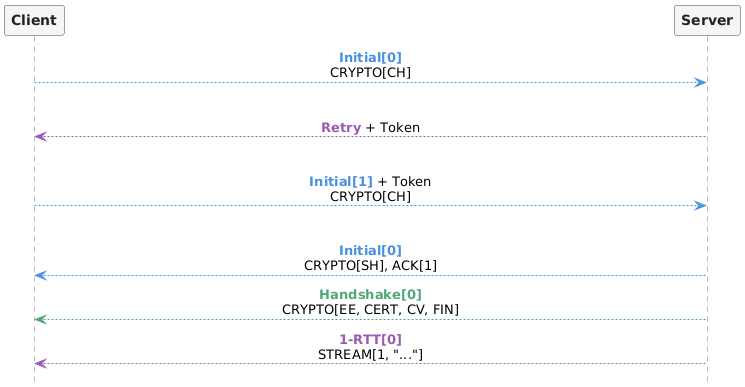
\includegraphics[width=0.7\linewidth]{fig/QUIC/quic_retry_with_token.png}
        \caption{Diagrama de tempo da validação de endereço com pacote \texttt{Retry}. Fonte: elaborado com base em \citep{rfc9000}.}
        \label{fig:quic_retry_with_token}
\end{figure}
 
O servidor também pode fornecer ao cliente, durante uma conexão estabelecida, um \textit{token} por meio do \textit{frame} \texttt{NEW\_\allowbreak{}TOKEN} \citep{rfc9000}. O cliente inclui esse \textit{token} no pacote \texttt{Initial} de uma conexão futura, o que permite ao servidor validar o endereço sem o RTT adicional do \texttt{Retry} e, assim, enviar respostas maiores, como as respostas a requisições 0-RTT, sem as restrições do limite de amplificação.

\subsection{Funcionamento dos \textit{Connection IDs}}
\label{sec:connection_ids_operation}

Os \textit{Connection IDs} permitem que o \textit{endpoint} receptor associe cada pacote à conexão correta independentemente dos endereços e das portas das camadas inferiores, que podem mudar ao longo da conexão. Cada \textit{endpoint} escolhe os identificadores pelos quais deseja ser endereçado: o DCID de um pacote corresponde ao identificador escolhido pelo receptor, e o SCID, ao identificador escolhido pelo emissor (Seção~\ref{sec:quic_headers}).

Ao longo da conexão, cada \textit{endpoint} fornece ao outro novos \textit{Connection IDs} por meio de \textit{frames} \texttt{NEW\_\allowbreak{}CONNECTION\_\allowbreak{}ID} e solicita o descarte dos antigos com \textit{frames} \texttt{RETIRE\_\allowbreak{}CONNECTION\_\allowbreak{}ID} \citep{rfc9000}. A troca de identificadores, em especial após uma migração de conexão, impede que um observador externo associe à mesma conexão pacotes enviados por caminhos diferentes. Para isso, um identificador não deve permitir sua correlação com os demais identificadores da mesma conexão, o que leva as implementações a gerá-los com um gerador de números pseudoaleatórios criptograficamente seguro (CSPRNG, \textit{Cryptographically Secure Pseudorandom Number Generator}).

Um \textit{endpoint} pode utilizar \textit{Connection IDs} de tamanho zero quando o endereço e a porta bastam para identificar a conexão. Nesse caso, porém, o \textit{endpoint} depende desses valores para associar os pacotes e perde o suporte a recursos como a migração de conexão e a tolerância a \textit{NAT rebinding}, relevantes para as técnicas de \textit{hole punching} discutidas na Seção~\ref{sec:quic_hole_punching}.

\cgk{Confirmar quando escrever sobre QUIC holepunching se isso realmente se aplica}

O ciclo de vida dos \textit{Connection IDs}, incluindo a emissão de novos identificadores e o momento de seu descarte, é definido no RFC~9000 \citep{rfc9000} e não é detalhado neste trabalho.

\section{Comunicação do QUIC}

Esta seção apresenta os mecanismos de comunicação entre os \textit{endpoints} de uma conexão QUIC. O protocolo multiplexa, em uma mesma conexão, \textit{streams} independentes entre si, e oferece entrega confiável e controle de fluxo. Esses mecanismos são descritos nas seguintes seções:

\begin{itemize}
    \item A Seção~\ref{sec:quic_streams} descreve a criação e o gerenciamento de \textit{streams};
    \item A Seção~\ref{sec:quic_acknowledgement} descreve os espaços de números de pacote e os mecanismos de confirmação de recebimento e de retransmissão;
    \item A Seção~\ref{sec:quic_flow_control} descreve o controle de fluxo;
    \item A Seção~\ref{sec:quic_connection_migration} descreve a migração de conexão após a mudança de endereço IP ou de porta de um dos \textit{endpoints}.
\end{itemize}

\subsection{\textit{Streams} do QUIC}
\label{sec:quic_streams}

Uma \textit{stream} é um canal ordenado de bytes dentro de uma conexão QUIC e pode ser unidirecional ou bidirecional \citep{rfc9000}. Cada \textit{stream} é identificada por um \textit{Stream ID}, um inteiro de 62 bits cujos dois bits menos significativos codificam o tipo da \textit{stream}: o bit menos significativo indica qual \textit{endpoint} a iniciou, e o segundo indica se ela é bidirecional ou unidirecional, conforme a Tabela~\ref{tab:quic_stream_types}. Assim, cada tipo dispõe de $2^{60}$ identificadores, atribuídos em incrementos de 4; as \textit{streams} bidirecionais iniciadas pelo cliente, por exemplo, recebem os identificadores 0, 4, 8 e assim por diante.

\begin{table}[ht]
    \centering
    \begin{tabular}{|c|l|}
        \hline
        \textbf{Bits} & \textbf{Tipo de \textit{stream}} \\
        \hline
        0x00 & Iniciada pelo cliente, bidirecional \\
        0x01 & Iniciada pelo servidor, bidirecional \\
        0x02 & Iniciada pelo cliente, unidirecional \\
        0x03 & Iniciada pelo servidor, unidirecional \\
        \hline
    \end{tabular}
    \caption{Tipos de \textit{stream} codificados nos dois bits menos significativos do \textit{Stream ID}. Fonte: \citep{rfc9000}.}
    \label{tab:quic_stream_types}
\end{table}

As \textit{streams} transportam dados de aplicação e podem ser encerradas normalmente pelo emissor, por meio do bit FIN do \textit{frame} \texttt{STREAM}, interrompidas pelo emissor, com o \textit{frame} \texttt{RESET\_\allowbreak{}STREAM}, ou ter sua recepção cancelada pelo receptor, com o \textit{frame} \texttt{STOP\_\allowbreak{}SENDING}. O QUIC garante a entrega confiável e ordenada dos bytes dentro de cada \textit{stream}, mas não impõe ordem entre \textit{streams} distintas. Assim, a perda de um pacote atrasa apenas as \textit{streams} cujos dados ele transportava, enquanto as demais continuam a entregar dados à aplicação, como ilustra a Figura~\ref{fig:quic_no_holb}. Esse mecanismo elimina o \textit{Head-of-Line Blocking} entre fluxos presente no HTTP/2 sobre TCP. O QUICv1 não define um esquema de priorização de \textit{streams}, mas recomenda que as implementações permitam à aplicação indicar a prioridade relativa de cada uma \citep{rfc9000}.

\begin{figure}[!ht]
        \centering
        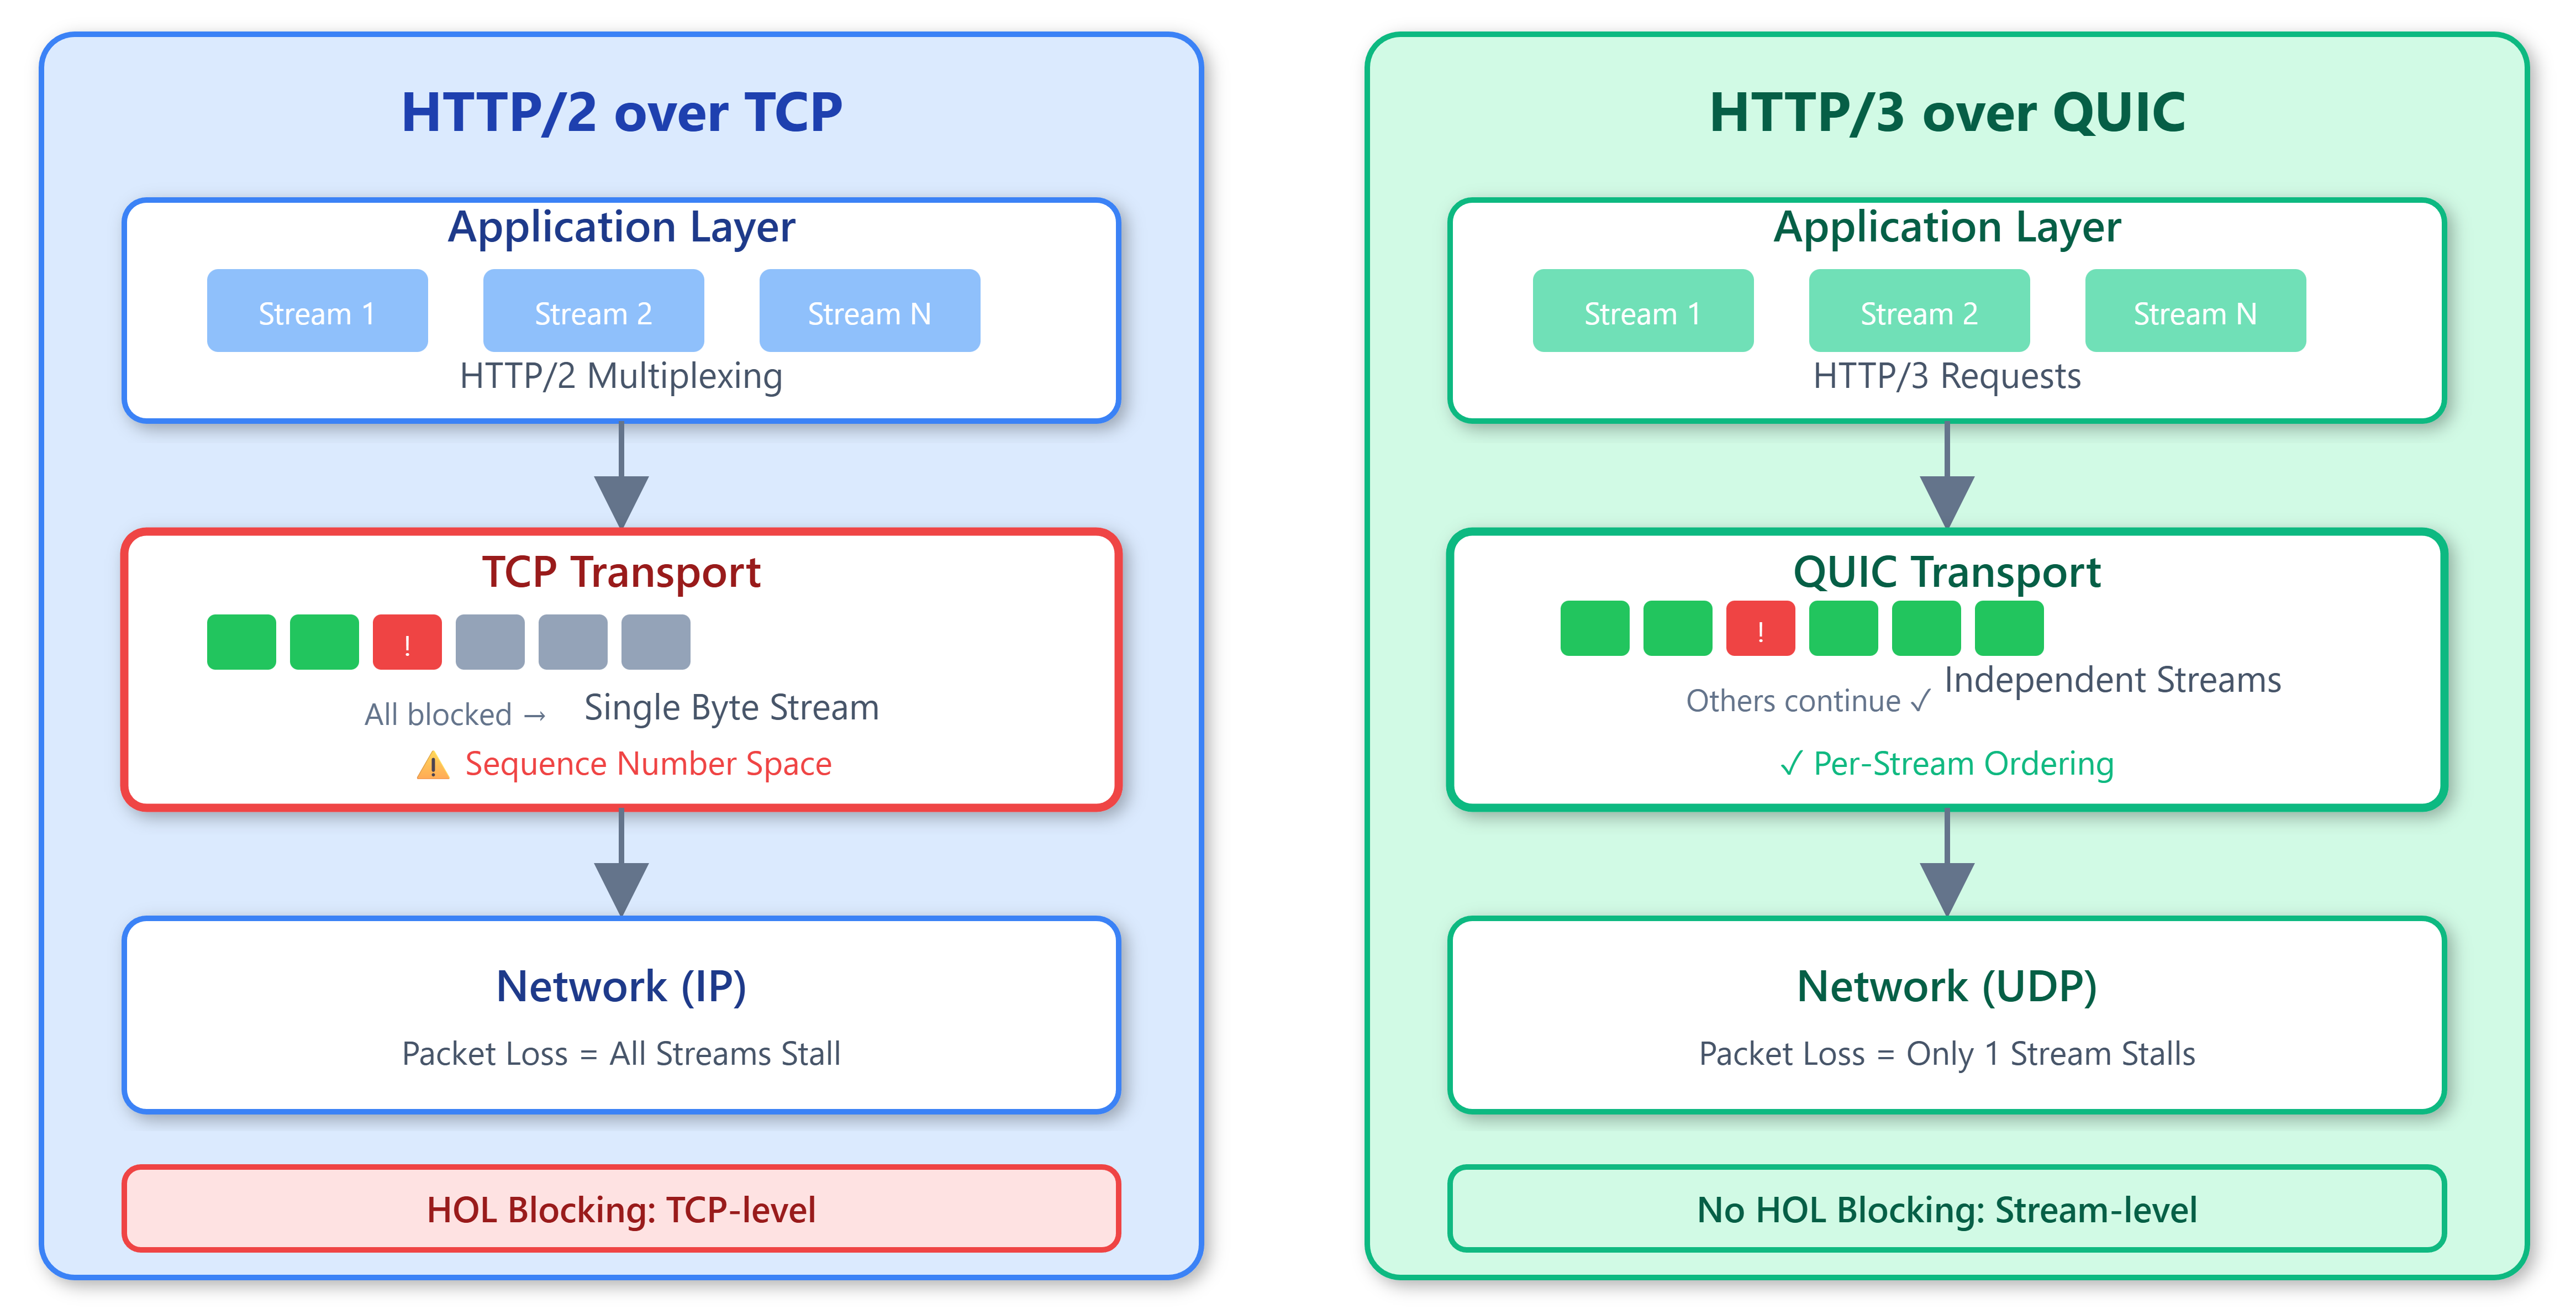
\includegraphics[width=0.9\linewidth]{fig/QUIC/quic_no_holb.png}
        \caption{Ausência de \textit{Head-of-Line Blocking} entre \textit{streams} no QUIC.}
        \label{fig:quic_no_holb}
\end{figure}

O RFC~9000 \citep{rfc9000} descreve o ciclo de vida de uma \textit{stream} por meio de duas máquinas de estados: uma para a parte de envio e outra para a parte de recepção. Em cada \textit{endpoint}, uma \textit{stream} unidirecional utiliza apenas uma dessas máquinas, enquanto uma \textit{stream} bidirecional utiliza ambas. Essas máquinas de estados servem apenas como referência: as implementações podem modelar seus estados internos de outra forma, desde que o comportamento observável seja consistente com a especificação. O detalhamento desses estados está fora do escopo deste trabalho.

\subsection{Confirmação de recebimento}
\label{sec:quic_acknowledgement}

Como descrito na Seção~\ref{sec:quic_packets}, um pacote QUIC pode conter vários \textit{frames}. Para fins de confirmação de recebimento, o pacote herda propriedades dos \textit{frames} que contém \citep{rfc9002}:

\begin{itemize}
    \item \textbf{Ack-eliciting:} pacote que contém ao menos um \textit{frame} diferente de \texttt{ACK}, \texttt{PADDING} e \texttt{CONNECTION\_\allowbreak{}CLOSE}. O receptor deve confirmar esse pacote imediatamente nos espaços \textit{Initial} e \textit{Handshake} e, no espaço \textit{Application Data}, em até \textit{max\_\allowbreak{}ack\_\allowbreak{}delay}, valor anunciado nos parâmetros de transporte;
    \item \textbf{Non-ack-eliciting:} pacote que contém apenas \textit{frames} \texttt{ACK}, \texttt{PADDING} ou \texttt{CONNECTION\_\allowbreak{}CLOSE}. O receptor não envia uma confirmação motivada apenas por esse pacote, mas o inclui nos intervalos do próximo \textit{frame} \texttt{ACK} que enviar por outro motivo.
\end{itemize}

Dessa forma, um pacote \textit{non-ack-eliciting} pode nunca ser confirmado, caso o receptor não tenha outro motivo para enviar um \textit{frame} \texttt{ACK}. A Tabela~\ref{tab:quic_ack_rules} resume as regras de envio de confirmações.

\begin{table}[ht]
    \centering
    \begin{tabular}{|p{0.72\textwidth}|c|}
        \hline
        \textbf{Situação} & \textbf{Permitido} \\
        \hline
        Responder a um pacote \textit{non-ack-eliciting} com um pacote \textit{non-ack-eliciting} enviado apenas para confirmá-lo & Não \\
        \hline
        Incluir um \textit{frame} \texttt{ACK} em um pacote que já seria enviado por outro motivo & Sim \\
        \hline
        Adiar a confirmação de um pacote \textit{non-ack-eliciting} até o recebimento de um pacote \textit{ack-eliciting} & Sim \\
        \hline
        Confirmar um pacote \textit{ack-eliciting} do espaço \textit{Application Data} em até \textit{max\_\allowbreak{}ack\_\allowbreak{}delay} & Sim \\
        \hline
    \end{tabular}
    \caption{Regras para o envio de confirmações no QUIC. Fonte: elaborado com base em \citep{rfc9000}.}
    \label{tab:quic_ack_rules}
\end{table}

Esse atraso permite ao receptor confirmar vários pacotes com um único \textit{frame} \texttt{ACK}, o que reduz a sobrecarga de confirmações.

No QUIC, a retransmissão não reenvia pacotes, mas as informações neles contidas, em novos pacotes com novos números \citep{rfc9002}. Cada tipo de \textit{frame} segue uma regra própria: os dados de \textit{streams} são reenviados em novos \textit{frames} \texttt{STREAM}, enquanto informações obsoletas, como \textit{frames} \texttt{ACK} antigos, não são retransmitidas. Como os números de pacote nunca se repetem em um mesmo espaço de numeração, o emissor distingue a confirmação de uma transmissão original da confirmação de uma retransmissão, ambiguidade presente no TCP. Essa regra também evita a reutilização de \textit{nonces} na proteção de pacotes (Seção~\ref{sec:quic_packet_protection}). A Seção~\ref{sec:quic_packet_numbers} discute os espaços de números de pacote; os algoritmos de detecção de perda e de retransmissão, definidos no RFC~9002 \citep{rfc9002}, estão fora do escopo deste trabalho.

Os \textit{frames} \texttt{ACK} descrevem intervalos de números de pacote recebidos (\textit{ACK Ranges}), e cada novo \textit{frame} \texttt{ACK} repete os intervalos já informados enquanto o receptor não souber que o emissor os recebeu, ou seja, até que o pacote que transportava esse \textit{frame} \texttt{ACK} seja confirmado \citep{rfc9000}. Assim, a perda de um pacote com um \textit{frame} \texttt{ACK} não exige retransmissão, pois o \textit{frame} \texttt{ACK} seguinte contém as mesmas informações. Como esses intervalos poderiam crescer indefinidamente, o receptor pode deixar de informar intervalos antigos para limitar o tamanho do \textit{frame}, ao custo de possíveis retransmissões desnecessárias pelo emissor.

\subsubsection{Números de pacote do QUIC}
\label{sec:quic_packet_numbers}

Os números de pacote variam de 0 a $2^{62}-1$, mas o cabeçalho transporta apenas seus bits menos significativos, em um campo de 1 a 4 bytes \citep{rfc9000}. O emissor escolhe o tamanho desse campo de modo a cobrir o dobro do intervalo entre o número do pacote atual e o maior número confirmado pelo receptor, e o receptor reconstrói o número completo a partir do maior número já recebido. Os números de pacote são organizados em três espaços:

\begin{itemize}
    \item \textbf{Initial:} pacotes \texttt{Initial};
    \item \textbf{Handshake:} pacotes \texttt{Handshake};
    \item \textbf{Application Data:} pacotes \texttt{0-RTT} e \texttt{1-RTT}.
\end{itemize}

Cada espaço possui numeração própria e é protegido por chaves distintas, o que separa criptograficamente os pacotes de cada fase da conexão. Em cada espaço, os números de pacote crescem monotonicamente e nunca são reutilizados. Se um \textit{endpoint} esgotar os números disponíveis, atingindo $2^{62}-1$, ele deve encerrar a conexão sem enviar um \textit{frame} \texttt{CONNECTION\_\allowbreak{}CLOSE}; para continuar a comunicação, é necessário estabelecer uma nova conexão.

\subsection{Controle de fluxo}
\label{sec:quic_flow_control}

O controle de fluxo do QUIC limita a quantidade de dados que o emissor pode enviar antes que o receptor os consuma, o que restringe a memória de \textit{buffer} necessária no receptor \citep{rfc9000}. O controle opera em dois níveis: cada receptor anuncia quantos bytes aceita receber em cada \textit{stream} e no conjunto de todas as \textit{streams} da conexão. De forma análoga, cada \textit{endpoint} limita o número de \textit{streams} que o outro pode abrir.

Os limites iniciais são anunciados nos parâmetros de transporte durante o \textit{handshake}. Os limites de dados correspondem a \textit{offsets} absolutos e só podem aumentar: o receptor os amplia à medida que consome os dados, por meio dos \textit{frames} \texttt{MAX\_\allowbreak{}STREAM\_\allowbreak{}DATA}, para uma \textit{stream}, e \texttt{MAX\_\allowbreak{}DATA}, para a conexão, e ignora qualquer \textit{frame} que anuncie um valor menor que o vigente. Quando o emissor é bloqueado por um desses limites, recomenda-se que ele envie um \textit{frame} \texttt{STREAM\_\allowbreak{}DATA\_\allowbreak{}BLOCKED} ou \texttt{DATA\_\allowbreak{}BLOCKED}, respectivamente, para informar o receptor. O limite de \textit{streams} é ampliado com \textit{frames} \texttt{MAX\_\allowbreak{}STREAMS}, que indicam o número total de \textit{streams} de cada tipo que podem ser abertas ao longo da conexão.

\subsection{Migração de conexão}
\label{sec:quic_connection_migration}

A migração de conexão (\textit{Connection Migration}) permite que uma conexão QUIC sobreviva à mudança do endereço IP ou da porta de um dos \textit{endpoints}, pois a conexão é identificada pelos \textit{Connection IDs}, e não pela quádrupla de endereços e portas \citep{rfc9000}. No QUICv1, apenas o cliente pode migrar a conexão; o servidor pode, no máximo, indicar um endereço preferencial durante o \textit{handshake}. A migração só é permitida após a confirmação do \textit{handshake} e se o servidor não tiver desabilitado o recurso pelo parâmetro de transporte \texttt{disable\_\allowbreak{}active\_\allowbreak{}migration}. Ao receber pacotes de um novo endereço, o \textit{endpoint} valida o novo caminho por meio dos \textit{frames} \texttt{PATH\_\allowbreak{}CHALLENGE} e \texttt{PATH\_\allowbreak{}RESPONSE}, descritos a seguir.

\subsubsection{Validação de caminho}
\label{sec:quic_path_validation}

Na validação de caminho (\textit{path validation}), o \textit{endpoint} que deseja verificar a alcançabilidade do outro \textit{endpoint} por um novo caminho envia, por esse caminho, um \textit{frame} \texttt{PATH\_\allowbreak{}CHALLENGE} com 8 bytes imprevisíveis \citep{rfc9000}. O outro \textit{endpoint} responde com um \textit{frame} \texttt{PATH\_\allowbreak{}RESPONSE} que repete esses bytes, e o recebimento de uma resposta correta valida o caminho. Os datagramas que transportam \texttt{PATH\_\allowbreak{}CHALLENGE} devem ter ao menos 1200 bytes, o que também verifica se o caminho suporta esse tamanho, respeitado o limite de amplificação descrito na Seção~\ref{sec:quic_address_validation}. O \textit{endpoint} pode enviar novos \textit{frames} \texttt{PATH\_\allowbreak{}CHALLENGE} para tolerar perdas. A Figura~\ref{fig:quic_path_validation} ilustra esse processo.

\begin{figure}[!ht]
        \centering
        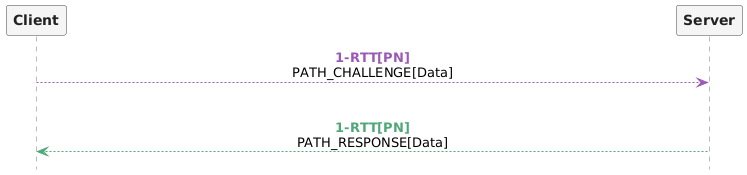
\includegraphics[width=0.7\linewidth]{fig/QUIC/quic_path_validation.png}
        \caption{Diagrama de tempo da validação de caminhos com o QUIC.}
        \label{fig:quic_path_validation}
\end{figure}

Esse processo se assemelha às verificações de conectividade do ICE (Seção~\ref{sec:ice}). O RFC~9000, no entanto, afirma que a validação de caminho não foi projetada como mecanismo de travessia de NAT. Ainda assim, a semelhança motivou propostas como a de \citep{draft-seemann-quic-nat-traversal}, que estende a validação de caminho, inclusive permitindo que o servidor a inicie, com o objetivo de viabilizar o \textit{hole punching} diretamente sobre o QUIC.

\subsubsection{Funcionamento da migração de conexão}
\label{sec:quic_connection_migration_process}

Para migrar, o \textit{endpoint} precisa dispor de um \textit{Connection ID} ainda não utilizado, fornecido pelo outro \textit{endpoint} (Seção~\ref{sec:connection_ids_operation}), que passa a ser usado como DCID no novo caminho. Essa troca impede que um observador correlacione os pacotes enviados antes e depois da migração. Se o outro \textit{endpoint} utilizar \textit{Connection IDs} de tamanho zero, a conexão fica associada ao endereço e à porta, e o tráfego nos dois caminhos se torna correlacionável; por isso, o \textit{endpoint} não deve iniciar a migração nesse caso.

Os pacotes trocados durante uma migração classificam-se em \textit{probing} e \textit{non-probing} \citep{rfc9000}. Um pacote \textit{probing} contém apenas \textit{frames} \texttt{PATH\_\allowbreak{}CHALLENGE}, \texttt{PATH\_\allowbreak{}RESPONSE}, \texttt{NEW\_\allowbreak{}CONNECTION\_\allowbreak{}ID} e \texttt{PADDING}, e serve para sondar um caminho sem migrar a conexão. Qualquer outro pacote é \textit{non-probing}; quando o servidor recebe, a partir de um novo endereço, um pacote \textit{non-probing} com o maior número de pacote já recebido, ele passa a utilizar esse endereço como destino, o que efetiva a migração.

Este trabalho distingue dois tipos de migração, denominação que não consta do RFC~9000. Na migração intencional, o cliente valida previamente o novo caminho com pacotes \textit{probing} e, em seguida, passa a enviar pacotes \textit{non-probing} por ele; o cliente pode também validar um caminho apenas para utilizá-lo posteriormente. Na migração não intencional, o endereço do cliente muda sem que ele o perceba, como em um \textit{NAT rebinding}, no qual o NAT altera o mapeamento de endereço ou de porta associado ao cliente, em geral após um período de inatividade. Nesse caso, o servidor recebe pacotes \textit{non-probing} de um novo endereço, passa a enviar pacotes a esse endereço, sujeito ao limite de amplificação, e inicia a validação do novo caminho. As Figuras~\ref{fig:quic_intentional_migration} e~\ref{fig:quic_non_intentional_migration} ilustram os dois casos.

\begin{figure}[ht]
    \centering
    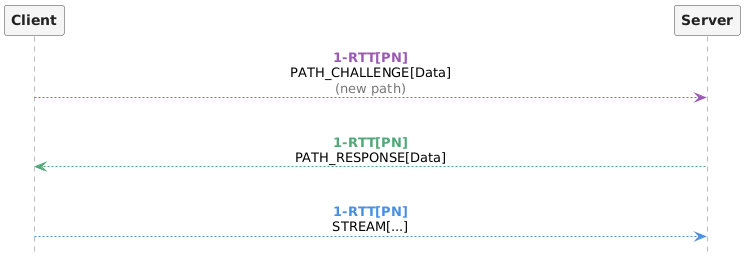
\includegraphics[width=0.6\textwidth]{fig/QUIC/quic_intentional_connection_migration.png}
    \caption{Diagrama de tempo da migração de conexão intencional.}
    \label{fig:quic_intentional_migration}
\end{figure}

\begin{figure}[ht]
    \centering
    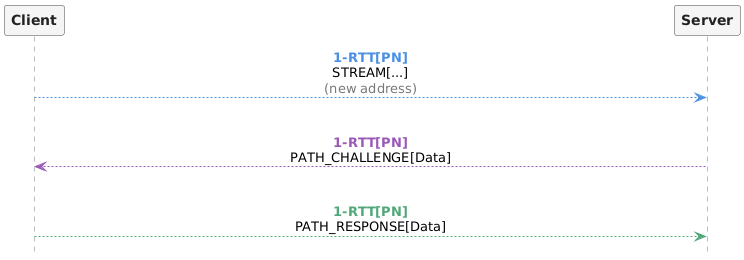
\includegraphics[width=0.6\textwidth]{fig/QUIC/quic_non_intentional_connection_migration.png}
    \caption{Diagrama de tempo da migração de conexão não intencional.}
    \label{fig:quic_non_intentional_migration}
\end{figure}

\section{QUIC Hole Punching}
\label{sec:quic_hole_punching}

O QUIC possui propriedades que favorecem técnicas de travessia de NAT. Por operar sobre UDP, beneficia-se do comportamento dos NATs que torna o \textit{hole punching} UDP mais eficaz que o TCP (Seção~\ref{sec:udp_hole_punching}). Além disso, a validação de caminho e a migração de conexão, embora não tenham sido projetadas para esse fim, podem apoiar essas técnicas (Seção~\ref{sec:quic_path_validation}).

Entre as propostas existentes, \citep{draft-seemann-quic-nat-traversal} apresenta duas formas de travessia de NAT com o QUIC.

A primeira utiliza o ICE (Seção~\ref{sec:ice}) sem alterações no QUIC e exige apenas que pacotes QUIC e STUN possam ser demultiplexados na mesma porta. Os \textit{peers} coletam seus candidatos ICE, trocam-nos por meio de um servidor de sinalização e executam as verificações de conectividade do ICE (Seção~\ref{sec:ice_connectivity_checks}). Concluído o \textit{hole punching}, os \textit{peers} estabelecem a conexão QUIC pelo par de candidatos selecionado.

A segunda abordagem integra a travessia de NAT ao próprio QUIC, com modificações em \textit{frames} e no processo de validação de caminho (Seção~\ref{sec:quic_path_validation}). Nessa abordagem, cliente e servidor estabelecem inicialmente uma conexão por meio de um terceiro servidor com endereço público, como um \textit{relay} ou \textit{proxy}. O cliente obtém seus candidatos de endereço, e o servidor anuncia os seus ao cliente por meio de um novo tipo de \textit{frame}. O cliente define a ordem de teste dos candidatos e sinaliza ao servidor o início do \textit{hole punching}; ambos iniciam então, simultaneamente, a validação de caminho para o mesmo par de candidatos, o que abre os mapeamentos nos NATs de ambos os lados. Trabalhos como \citep{draft-bruynooghe-n0-quic-nat-traversal} estendem essa abordagem com técnicas como o QUIC \textit{multipath} \citep{draft-quic-multipath-06}.

Essa abordagem exige alterações no protocolo, como três novos tipos de \textit{frame}, e permite que o servidor inicie a validação de caminho, o que o RFC~9000 não admite. O próprio \textit{draft} reconhece que essa extensão expõe a conexão a um risco semelhante ao de ataques de amplificação, sem apresentar uma mitigação completa.

Além dessas propostas, \citep{liang2024nat} compara técnicas de \textit{hole punching} TCP (Seção~\ref{sec:tcp_hole_punching}) e QUIC. Até a escrita deste trabalho, entretanto, o IETF não publicou nenhum RFC sobre travessia de NAT com o QUIC, e questões como o risco de amplificação permanecem em aberto.

\begin{comment}
    
\section{QUIC para Aplicações P2P}

\cgk{verificar se isso não vai pra outro lugar}

\subsection{QUIC para Aplicações P2P real-time}

\subsection{QUIC para Aplicações P2P IoT}

\end{comment}

\chapter{Integração de uma Arquitetura de Transporte QUIC sobre ICE}
\label{chap:implementation}

Este capítulo descreve o desenvolvimento da comunicação entre \textit{peers} atrás de um NAT através das técnicas de \textit{NAT traversal} vistas na Seção~\ref{sec:nat_traversal}, com enfoque nas etapas de \textit{hole punching} baseadas nos métodos que utilizam o protocolo de transporte UDP, estendendo-se a um uso do protocolo QUIC para realizar a mesma comunicação, utilizando a biblioteca \texttt{OpenSSL} \citep{openssl_quic}.

A partir do protocolo Chownat, visto na Seção~\ref{sec:chownat}, e da configuração de topologias vistas na Seção~\ref{sec:topologies}, em ambientes de simulação descritos na Seção~\ref{sec:simulation_environments}, foi realizada uma tradução e extensão deste protocolo, de forma a permitir maior estabilidade nas etapas de comunicação (como visto na Seção~\ref{sec:chownat_translation_extension}), a partir de uma interface genérica para realização de \textit{hole punching} (vista na Seção~\ref{sec:hole_punching_protocols}).

Além disso, esta solução foi generalizada para permitir o uso do protocolo ICE na obtenção de candidatos e na realização do \textit{hole punching}, como descrito na Seção~\ref{sec:ice_library}. Também é descrito o uso da biblioteca \texttt{libnice} para essa integração, que passa a ter a possibilidade de assumir a manipulação das \textit{sockets} de comunicação, antes feita diretamente pela interface genérica, tanto para protocolos genéricos (como o Chownat) quanto para a própria OpenSSL.

A implementação descrita neste capítulo é executada nos \textit{gateways} da arquitetura proposta. Nos ambientes de teste, esses \textit{gateways} são representados por \textit{hosts} de propósito geral, nos quais também executam as aplicações TCP locais. Os roteadores da topologia desempenham funções de encaminhamento e, quando configurados para isso, de NAT; não são os equipamentos nos quais a implementação é executada.

\section{Topologias}
\label{sec:topologies}

As topologias foram desenvolvidas a fim de realizar a validação das técnicas de hole punching a partir testes dos protocolos abordados na seção \ref{sec:hole_punching_protocols}. 

Nas topologias apresentadas nesta seção, os \textit{peers} representam os \textit{gateways} que executam a infraestrutura de comunicação proposta na Seção \ref{sec:protocol_stack}. Os dispositivos e as aplicações locais associados a esses nós não são representados nos diagramas, pois o foco está no transporte entre os \textit{gateways}.

\subsection{Topologia Simples para Hole Punching}
\label{sec:basic_topology_hole_punching}

A topologia utilizada como base nos testes das técnicas de UDP \textit{hole punching} (vistas na Seção~\ref{sec:udp_hole_punching}) foi baseada em um cenário simples, no qual cada \textit{peer} vive abaixo de um único NAT. Este cenário é capaz de exercitar o funcionamento do \textit{hole punching} em si, sem depender completamente do correto funcionamento dos NATs. Isto também simplifica as etapas de configuração dos ambientes de simulação para cada caso.

Esta topologia, que pode ser vista na Figura~\ref{fig:basic_topology}, viabiliza os testes efetivos de \textit{hole punching}. Entretanto, ela não foi projetada pensando em simulações para uso do ICE; apesar disso, também pode ser reaproveitada para esse propósito, bastando atribuir uma função específica ao servidor. No modelo original desta topologia, o servidor não possui função alguma, e os \textit{peers} já conhecem previamente os IPs públicos um do outro. Além disso, como já visto anteriormente (na Seção~\ref{sec:chownat}), dado que o endereço é necessariamente pré-conhecido, as portas públicas (que também fazem parte do endereço público) precisam ser traduzidas exatamente para a porta de origem (porta na qual a \textit{socket} fez a operação de \textit{bind}), de forma que não seja necessário nenhum mecanismo de predição de portas, descrito na Seção~\ref{sec:udp_hole_punching_edm}.

\begin{figure}[ht]
    \centering
    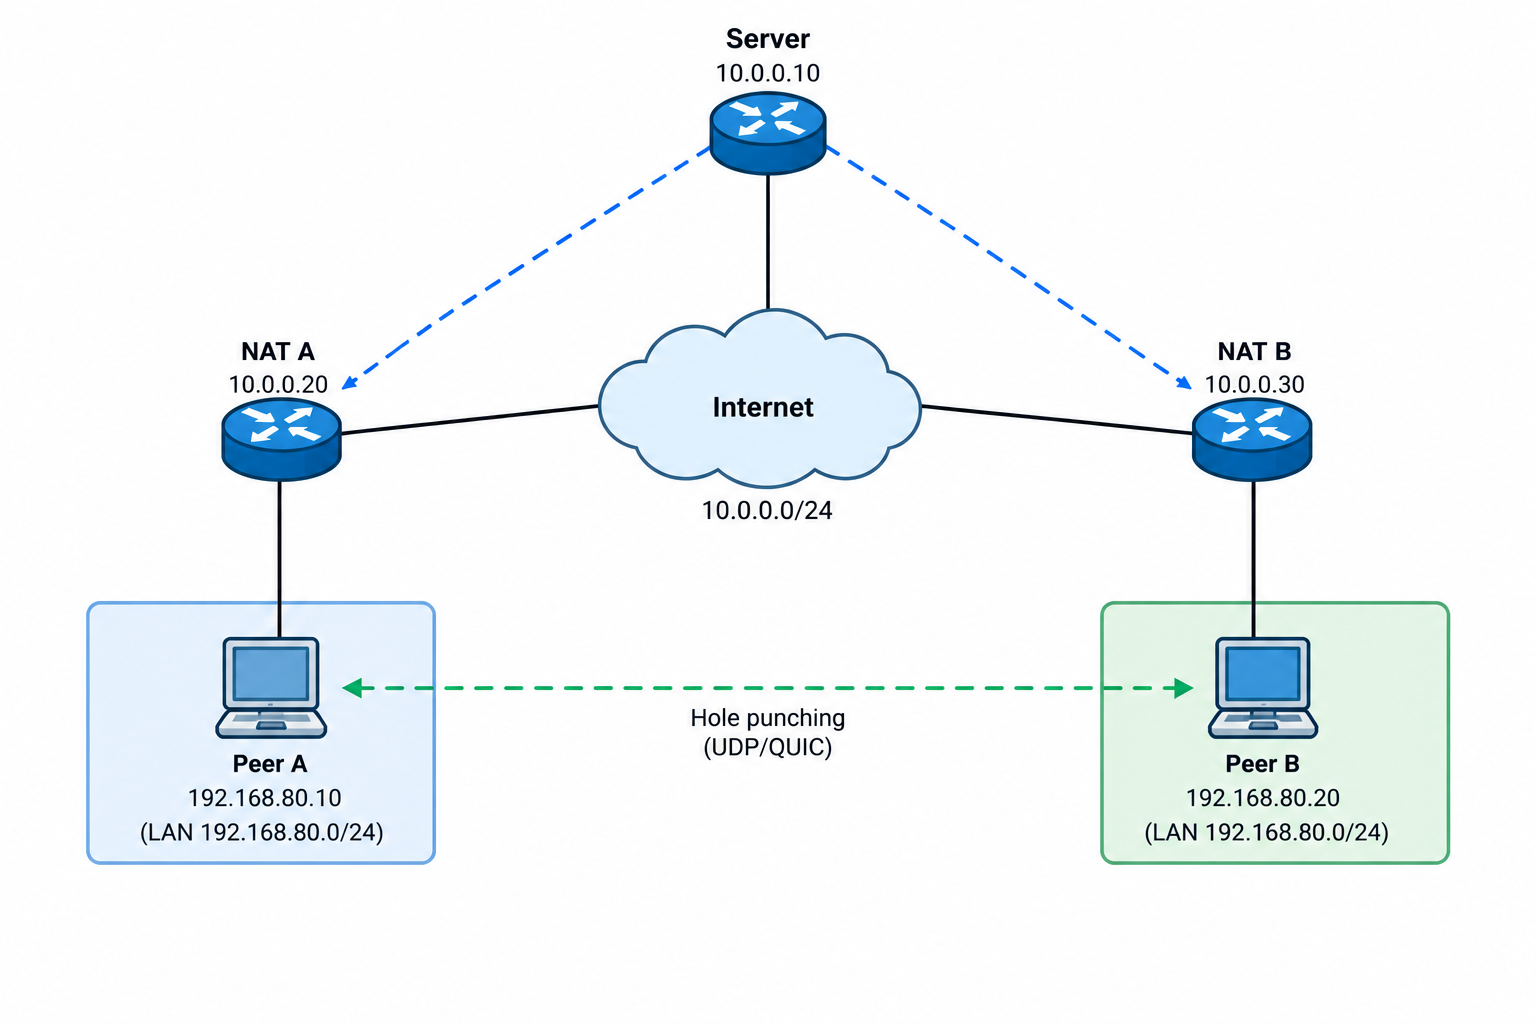
\includegraphics[width=0.8\textwidth]{fig/implementation/topologies/basic_topology.png}
    \caption{Topologia simples para realização de \textit{hole punching}.}
    \label{fig:basic_topology}
\end{figure}

\subsection{Topologia para Hole Punching Utilizando o Protocolo ICE}
\label{sec:ice_topology}

Nesta topologia, os roteadores possuem as mesmas responsabilidades e configurações de NATs  como esperado pelo próprio intuito de uso do ICE de forma a reaproveitar dispositivos já existentes sem que haja a necessidade de alteração destes. Entretanto, os \textit{peers} e o servidor (Server da Figura \ref{fig:basic_topology} obterão novas responsabilidades associas ao processo de estabelecimento de candidatos ICE.

Os \textit{peers} serão incumbidos da responsabilidades associadas a obtenção de candidatos ICE, Essa obtenção, como visto anteriormente na Seção \ref{sec:ice} é possível a partir do protocolo STUN, do protocolo TURN, IPs das interfaces locais, e também IPs descobertos durante a fase dos \textit{connectivity checks}. O \citep{rfc8838} também descreve que estes candidatos não estão limitados a esse escopo e também podem ser obtidos por outros meios. A partir desta obtenção de candidatos, os \textit{peers} também terão a responsabilidade de trocar os IPs candidatos entre si a partir de um servidor de sinalização, que, como descrito anteriormente na Seção \ref{sec:ice}, não faz parte da espectativa do próprio protocolo, portanto uma solução genérica pode ser utilizada (servidor MQTT, servidor HTTP/WebSockets, etc...). E como responsabilidade final, estes \textit{peers} também precisarão realizar os \textit{connectivity checks} do ICE afim de encontrar um possível candidato para a comunicação.

O servidor, nesta topologia, obterá as responsabilidades faltantes para a conclusão do protocolo ICE, portanto este servidor será responsável pela gerência de um servidor STUN, um servidor TURN, e também um servidor de sinalização, a fim de prover os serviços necessários para realização de testes de funcionalidade sobre a implementação proposta entre os demais protocolos.

A topologia continua a mesma, entretanto as responsabilidades aumentam e são dispostas como vistas na Figura \ref{fig:ice_topology}.

\begin{figure}[ht]
    \centering
    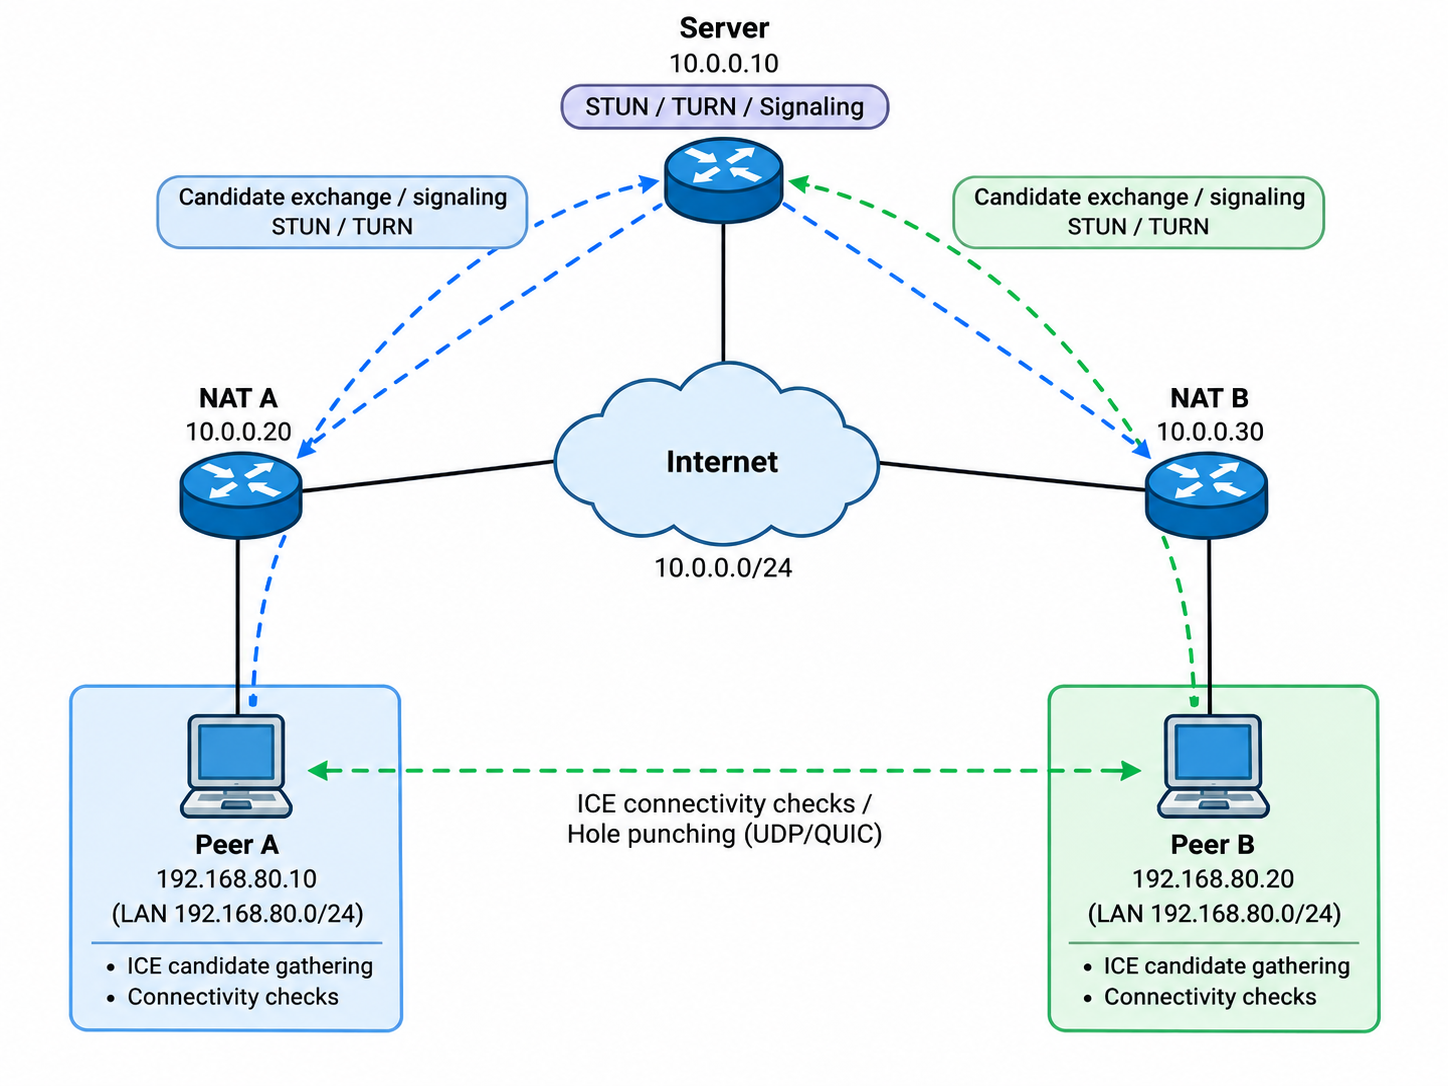
\includegraphics[width=0.8\textwidth]{fig/implementation/topologies/ice_topology.png}
    \caption{Topologia para realização de \textit{hole punching} utilizando o protoclo ICE.}
    \label{fig:ice_topology}
\end{figure}

\section{Ambientes de Simulação}
\label{sec:simulation_environments}

Para a validação das técnicas de \textit{hole punching} utilizando os protocolos propostos na Seção~\ref{sec:hole_punching_protocols}, diferentes ambientes de simulação de rede foram avaliados antes da definição da topologia final de testes (vista na Seção~\ref{sec:topologies}).


\subsection{Ambiente de Simulação GNS3}

O GNS3, ou \textit{Graphical Network Simulator-3}, disponível em \citep{gns3}, é um simulador amplamente utilizado para simulação de redes, permitindo a emulação de dispositivos de rede virtualizados em topologias complexas.

Este simulador foi o primeiro a ser utilizado, devido à familiaridade e ao uso prévio dele em projetos anteriores voltados à universidade. Além disso, a interface gráfica e a integração com o \textit{Wireshark} (ferramenta utilizada para \textit{sniffing} de rede) providas por ele facilitam a análise visual dos pacotes transmitidos, auxiliando na verificação do correto funcionamento das transmissões.

Entretanto, esta ferramenta deixou de ser utilizada à medida que os testes dos protocolos se tornaram mais intensos, devido à sua limitação de integração com o \textit{build system} CMake (ferramenta geradora de sistemas de \textit{build}) desenvolvido para este trabalho, dificultando a automação de testes de regressão.

\subsubsection{Máquinas Virtuais Utilizadas no GNS3}

Para os testes utilizando o GNS3, foram utilizadas máquinas virtuais para simular cada \textit{peer}, NAT e servidor das topologias propostas. Os componentes virtualizados utilizados foram os seguintes:

\begin{itemize}
    \item \textbf{Debian 12.6:} Máquina Debian utilizada para roteadores genéricos e \textit{hosts}, a fim de facilitar a execução de \textit{scripts} e a instalação de bibliotecas;
    \item \textbf{Cisco IOSv 15.9:} Máquina Cisco utilizada como roteador para a simulação e configuração de NATs;
    \item \textbf{NAT:} Componente nativo do GNS3 que simula um NAT de rede. Este componente não é utilizado como NAT alvo do \textit{hole punching}, mas sim para distribuir acesso à internet aos dispositivos internos da topologia, dado que alguns deles necessitam de internet para a instalação de bibliotecas.
\end{itemize}

\subsubsection{Configuração da Topologia Simples para Hole Punching no GNS3}
\label{sec:basic_topology_gns3}

A topologia configurada pode ser vista na Figura~\ref{fig:basic_topology_gns3}. Ela utiliza dois roteadores com NAT de ``mapeamento espelhado'' de porta origem, dois clientes e um servidor (utilizado apenas como \textit{stub} neste momento). Este ``mapeamento espelhado'' se refere ao mapeamento citado na Seção~\ref{sec:basic_topology_hole_punching}, no qual a porta pública é traduzida para a porta de origem. Isso permite que as portas traduzidas sejam conhecidas previamente; do contrário, não seria possível realizar \textit{hole punching} sem a existência de um servidor como o servidor STUN.

\begin{figure}[ht]
    \centering
    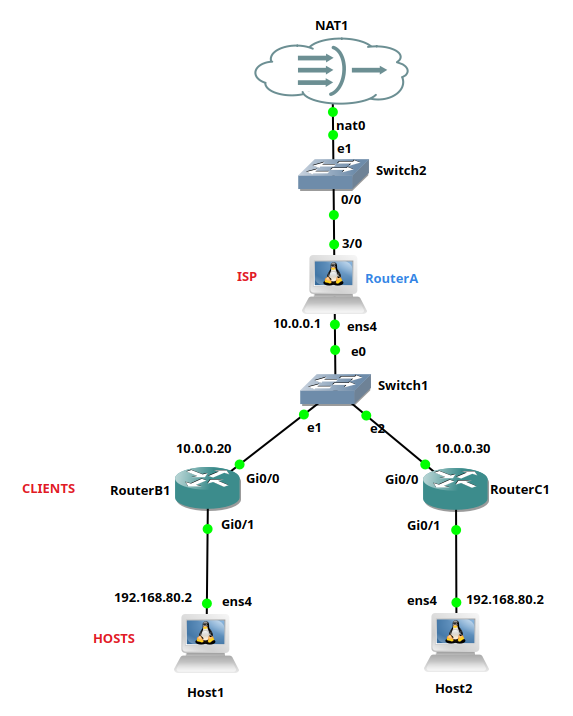
\includegraphics[width=0.6\textwidth]{fig/implementation/gns3/basic_topology_gns3.png}
    \caption{Topologia simples desenvolvida no GNS3.}
    \label{fig:basic_topology_gns3}
\end{figure}

Nesta topologia, todos os \textit{hosts} utilizam o sistema operacional Debian, e cada um deles atua como um \textit{peer} do cenário de \textit{hole punching}. Os NATs são roteadores Cisco IOSv, cada um configurado com um IP público fixo e com mapeamento de portas espelhado em relação à porta dos pacotes de saída, como descrito anteriormente. O ISP é um roteador que, nesta topologia, atua apenas como \textit{stub}, sem participar do \textit{hole punching}, servindo somente como servidor DHCP para os roteadores NAT em uma rede \texttt{10.0.0.0/24}. Já o componente \texttt{NAT1} serve apenas para prover acesso à internet a todos os \textit{peers} abaixo dele.

\begin{comment}
    
\subsubsection{Configuração da Topologia ICE para Hole Punching no GNS3}

Escrever quanto tiver a implementação

\cgk{Implementar a configuração, mas acho que não vale a pena perder tempo}

\end{comment}

\subsection{Linux Network Namespaces}
\label{sec:linux_network_namespaces}

Os \textit{Linux Network Namespaces} (vistos em \citep{linux-network-namespaces}) permitem configurar ambientes de teste na máquina local, utilizando apenas interfaces virtualizadas na comunicação. Os \textit{namespaces} compartilham o mesmo \textit{kernel}, mas possuem isolamento dos recursos de rede, como pode ser visto na Figura~\ref{fig:namespaces_isolation}. Isso facilita a execução de testes de \textit{debug} e de regressão, permitindo a análise de alterações no código que afetam mais do que uma única biblioteca. Este mecanismo foi adotado como principal ambiente de testes devido à sua praticidade.

\begin{figure}[ht]
    \centering
    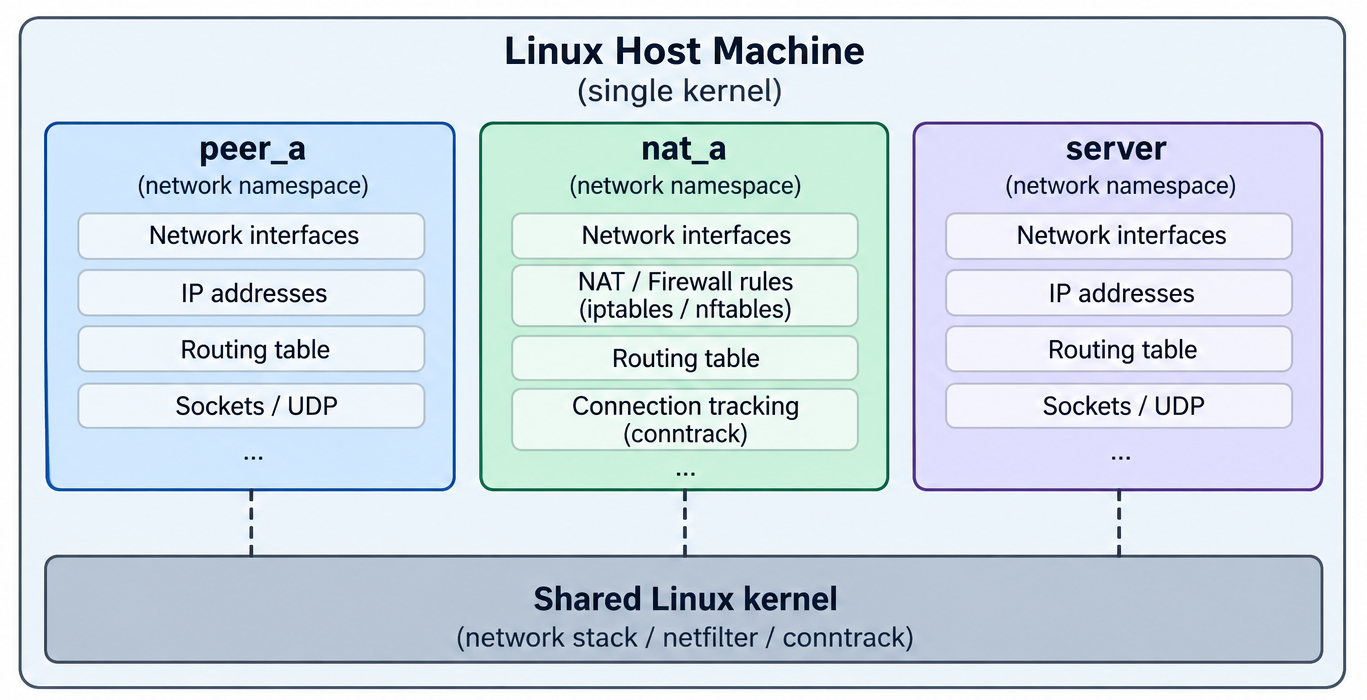
\includegraphics[width=0.8\textwidth]{fig/implementation/network_namespaces/namespaces_isolation.png}
    \caption{Isolamento dos \textit{Network Namespaces} no \textit{kernel} do Linux.}
    \label{fig:namespaces_isolation}
\end{figure}

Entretanto, a configuração nativa desses \textit{namespaces} é feita com o comando \texttt{ip}, que não é trivial de utilizar dado o grande conjunto de configurações possíveis. Por exemplo, para configurar um NAT, além de configurar as interfaces virtuais, é necessário um outro tipo de configuração, feita com o programa \texttt{iptables}. Além disso, a documentação é extensa e não existem perfis pré-configurados para tipos específicos de NAT, como o NAT com EIM ou o NAT com ``mapeamento espelhado''. Por isso, foi escolhido utilizar a biblioteca PatchBay \citep{patchbay}, desenvolvida em Rust, que permite a configuração completa do ambiente a partir de perfis de configuração previamente definidos. Isso facilita os testes e garante o comportamento esperado de cada configuração. Portanto, este trabalho utiliza este \textit{framework} como base das configurações de rede dos \textit{Linux Network Namespaces}.

Nesse ambiente, os nós representam os extremos da comunicação entre \textit{gateways}, sem reproduzir o hardware de dispositivos IoT. Como os \textit{namespaces} compartilham recursos da mesma máquina, os resultados devem ser interpretados de acordo com essa configuração. Os testes nesse ambiente permitem controlar as condições de rede e verificar o funcionamento da integração, enquanto eventual avaliação em hosts separados constitui outro ambiente experimental.

\subsubsection{Topologia Simples para Hole Punching Utilizando Linux Network Namespaces}
\label{sec:basic_topology_network_namespaces}

A topologia simples utilizando \textit{Linux Network Namespaces} é muito parecida com a vista na Figura~\ref{fig:basic_topology_gns3}. A diferença é que o PatchBay não permite a definição manual do IP de WAN dos roteadores NAT; em vez disso, cada roteador recebe um endereço fornecido pelo ISP (como visto na Listagem \ref{lst:patchbay_isp_config}, que neste caso pertence à mesma rede \texttt{10.0.0.0/24}. Cada roteador também atribui endereços IP à sua rede local (LAN) e configura um NAT do tipo \textit{Moderate}.

\begin{lstlisting}[caption={Configuração do ISP no PatchBay.}, label={lst:patchbay_isp_config}]
    let isp = lab
        .add_router("isp")
        .preset(RouterPreset::Public)
        .downstream_cidr("10.0.0.0/24".parse()?)
        .build()
        .await?;
\end{lstlisting}

O PatchBay \citep{patchbay} fornece quatro tipos de NAT para IPv4, além de um modo customizável (\textit{Custom}), de variações para IPv6 e de \textit{firewalls}:

\begin{itemize}
    \item \textbf{None:} Sem NAT, ou seja, um roteador sem qualquer tradução de endereços;
    \item \textbf{Open:} Implementa EIM e EIF, descritos na Seção~\ref{sec:nat_classification_by_translation_behavior}, correspondendo ao \textit{Full-Cone NAT};
    \item \textbf{Moderate:} Implementa EIM e APDF, correspondendo ao \textit{Port-Restricted Cone NAT}. Este é o comportamento típico de roteadores domésticos;
    \item \textbf{Strict:} Implementa EDM (\textit{Endpoint-Dependent Mapping}, com portas aleatórias) e APDF, correspondendo ao \textit{Symmetric NAT}. Quando ambos os \textit{peers} estão atrás desse tipo de NAT, o \textit{hole punching} direto não é possível, sendo necessário um \textit{relay}.
\end{itemize}

Portanto, a topologia implementada utiliza, nos roteadores (clients), o modo \textit{Moderate} como visto na Listagem \ref{lst:patchbay_client_config}, com a alteração de algumas regras de mapeamento para manter o ``mapeamento espelhado'', de modo que a porta traduzida seja, por padrão, a porta de origem do \textit{socket} (definida via \textit{bind}). Desta forma, os \textit{peers} podem permanecer em uma mesma rede local, que neste caso é a mesma vista na Figura~\ref{fig:basic_topology_gns3}, \texttt{192.168.80.0/24}.

\begin{lstlisting}[caption={Configuração de roteadores no PatchBay.}, label={lst:patchbay_client_config}]
    let router_a = lab
        .add_router("router_a")
        .preset(RouterPreset::Home)
        .upstream(isp.id())
        .downstream_cidr("192.168.80.0/24".parse()?)
        .nat(Nat::Moderate)
        .firewall(Firewall::None)
        .build()
        .await?;
\end{lstlisting}

\subsubsection{Configuração da Topologia ICE para Hole Punching utilizando Linux Network Namespaces}
\label{sec:ice_topology_network_namespaces}

A topologia para ICE mantém a disposição dos nós, o endereçamento das redes e o perfil NAT \textit{Moderate} utilizados na topologia básica, descrita na Seção~\ref{sec:basic_topology_network_namespaces}. As regras adicionais de tradução de portas, entretanto, dependem do cenário: os testes sem ICE preservam a porta de origem para permitir o conhecimento prévio dos endpoints públicos; os testes com ICE utilizam a descoberta desses endpoints, incluindo um caso com remapeamento explícito de portas, apresentado na Seção~\ref{sec:experimental_scenarios}. Entretanto, como visto na Seção~\ref{sec:ice_topology}, tanto o servidor quanto os \textit{peers} assumem novas responsabilidades. Na configuração da topologia em si, a configuração dos \textit{peers} não muda, dado que a biblioteca ICE estará integrada ao mesmo \textit{script} já executado anteriormente em cada \textit{peer}. O servidor, entretanto, passará a executar \textit{scripts} que vão além de sua funcionalidade anterior de apenas fornecer o serviço de DHCP.

O servidor passa a assumir duas novas responsabilidades. A primeira está associada ao fornecimento de serviços STUN e TURN, permitindo a cada \textit{peer} a obtenção de mais candidatos públicos a partir desses protocolos. Já a segunda está associada ao fornecimento de um serviço de sinalização, de forma que os \textit{peers} possam trocar candidatos entre si a fim de realizar suas verificações de conectividade.

Para o fornecimento dos serviços STUN e TURN, foi utilizada a biblioteca \texttt{coturn} \citep{coturn}, responsável por implementar serviços coerentes com os RFCs \citep{rfc8489} e \citep{rfc8656}, que trazem as informações mais atualizadas sobre os protocolos e obsoletam comportamentos antigos, tornando-se, portanto, uma solução adequada para a validação da implementação em questão.

Para o fornecimento do serviço de sinalização, o servidor será responsável por executar um \textit{script} simples que realiza a troca de informações entre os \textit{peers}. Este \textit{script} executa um servidor TCP que ouve em todas as interfaces na porta 5555 e aguarda a conexão dos dois \textit{peers}. Assim que os \textit{peers} se conectam, é iniciada a troca de informações entre eles, contendo os dados sobre os candidatos locais de cada \textit{peer}, obtidos por meio do servidor STUN/TURN ou de outro método, juntamente com as informações necessárias para a autenticação prevista no protocolo ICE.

\subsection{Infraestrutura controlada}

Configurar nos roteadores da Datacom...

\cgk{lembrar de adicionar se fizer configurações}

\section{Protocolos de Comunicação para Hole Punching}
\label{sec:hole_punching_protocols}

Este trabalho teve origem em um projeto realizado em conjunto com a Datacom, cujo objetivo era viabilizar a comunicação entre dois \textit{peers} com o mínimo de infraestrutura possível. % Opcional: Com o encerramento do projeto, o trabalho passou a ser continuado em caráter acadêmico, no contexto deste TCC.

Inicialmente, o objetivo era transmitir dados TCP, especificamente HTTP, por meio de técnicas de \textit{hole punching}. Dada a complexidade do TCP \textit{hole punching}, vista na Seção~\ref{sec:tcp_hole_punching}, optou-se pelo UDP \textit{hole punching}. Como base, foi utilizado o Chownat, que, além de realizar \textit{hole punching}, é capaz de tunelar dados TCP sobre UDP sem o custo dos pacotes de controle do TCP, permitindo uma comunicação direta e rápida entre os \textit{peers}.

Para a comunicação, foi proposto o uso de um servidor mínimo (\textit{rendezvous server}), responsável pela autenticação e pela troca de endereços IP entre os \textit{peers}, com função semelhante à de um servidor STUN no que diz respeito à descoberta de endereços. Também foi proposto o uso de um protocolo capaz de garantir os requisitos de dependabilidade e segurança descritos na introdução deste trabalho, tendo-se optado pelo QUIC, dada a sua recente expansão e a compatibilidade com os requisitos de transmissão de dados de aplicação do projeto.

A implementação da infraestrutura de servidores foi realizada apenas parcialmente durante o projeto, e pouco foi desenvolvido da comunicação entre dois \textit{peers} utilizando o QUIC. Este trabalho é também uma extensão do trabalho de Ivan [CITAR TCC DO IVAN], que abordou aspectos mais voltados à segurança e aos objetivos por trás da escolha do QUIC como protocolo ideal para os cenários propostos.

\cgk{Citar o TCC do Ivan}

\begin{comment}
    
No contexto de dispositivos IoT, que podem gerar grandes volumes de dados, a comunicação P2P é um cenário relevante, como descrito na introdução, principalmente em relação ao uso de banda e à necessidade de um servidor especializado para gerenciar o tráfego, além dos requisitos de dependabilidade e segurança para os usuários.

\cgk{Ver se realmente tem trabalhos de IoT relacionados com QUIC e citar aqui}
\end{comment}

No cenário IoT adotado neste trabalho, a comunicação externa é realizada pelos gateways, que executam as aplicações integradas ao túnel. O interesse está em interligar essas aplicações quando os gateways se encontram em redes distintas, utilizando os mecanismos de descoberta e seleção de caminhos disponíveis na solução. Os dados dos dispositivos são representados, nos experimentos, por mensagens geradas por aplicações locais.

Nesta seção são apresentadas as implementações e extensões desenvolvidas para viabilizar a comunicação com as técnicas de \textit{hole punching} propostas inicialmente, possibilitando uma comunicação direta entre dois \textit{peers} atrás de um NAT. 

\begin{itemize}
    \item A Seção \ref{sec:chownat_translation_extension} apresenta uma continuação da implementação desenvolvida durante o projeto;
    \item A Seção \ref{sec:ossl_quic_for_hole_punching} apresenta uma proposta de uso da biblioteca OpenSSL no modo \textit{threadless} para \textit{hole punching}; 
\end{itemize}

\subsection{Interface de transporte para hole punching}
\label{sec:hole_punching_interface}

A interface de transporte para \textit{hole punching} é uma interface criada especificamente para este trabalho, com o intuito de auxiliar a aplicação de múltiplos protocolos de transporte UDP na realização de \textit{hole punching}, independentemente de o protocolo possuir ou não esse recurso de forma nativa. Além disso, esta interface também tem como objetivo habilitar o tunelamento de TCP sobre protocolos de transporte UDP, de modo a transportar pacotes de serviços da camada de aplicação que utilizam TCP sobre protocolos de transporte diferentes.

Esta interface é baseada no Chownat (Seção~\ref{sec:chownat}) e propõe uma abordagem modular desse mesmo protocolo, a fim de permitir reutilizar sua estrutura na aplicação de \textit{hole punching} para outros protocolos, como o QUIC. Como objetivo principal, busca-se permitir o reuso dos componentes do protocolo original (as partes associadas à realização de \textit{hole punching} e ao tunelamento TCP), de forma a permitir apenas ``trocar peças'' e facilitar a integração de outros protocolos.

Esta interface também propõe uma abordagem \textit{threadless}, a partir de uma API baseada em eventos, similar à provida pela \texttt{libwebsockets} \citep{libwebsockets},
que serviu como inspiração para a API desenvolvida. Esta implementação baseada em eventos utiliza chamadas de sistema por meio da \textit{syscall} \texttt{select}, que permite a integração de múltiplos \textit{sockets} e a espera por novos dados recebidos neles.

Além disso, esta interface também permite um modelo de configuração que possibilita a gerência tanto da configuração quanto do uso de \textit{hole punching}, bem como do uso de tunelamento TCP. Isto é feito de forma prévia ao início real da conexão do protocolo, o que também favorece a arquitetura modular.

\subsubsection{Configuração da interface}

A configuração da interface permite, assim como o próprio Chownat visto anteriormente, a existência de duas sessões: uma sessão UDP e uma sessão TCP, possibilitando o tunelamento.

Cada sessão possui configurações específicas para a devida conexão, como \textit{timeouts} e endereços de origem e destino. Isto permite que uma aplicação que utilize esta interface possa configurá-la previamente a partir de dados obtidos de forma externa, como, por exemplo, a partir do ICE.

A configuração também permite o registro de uma \textit{callback}, que será chamada a cada novo evento, passando como parâmetro o \textit{reason} (motivo) do evento específico.

Para fornecer uma organização baseada no paradigma de orientação a objetos, a configuração também permite que seja escolhida uma implementação específica de protocolo que utilizará a sessão UDP. Isso significa que um novo protocolo UDP que deseje utilizar esta mesma interface precisa apenas implementar um conjunto de funções pré-definidas, simulando o comportamento de uma tabela virtual. Na prática, essa tabela é representada por um conjunto de ponteiros de função, que devem ser implementados por cada implementação de protocolo UDP com interesse em utilizar a interface. A API pública da interface pode ser observada diagrama de blocos visto na Figura \ref{fig:udp_conn_diagram}.

\begin{figure}[ht]
    \centering
    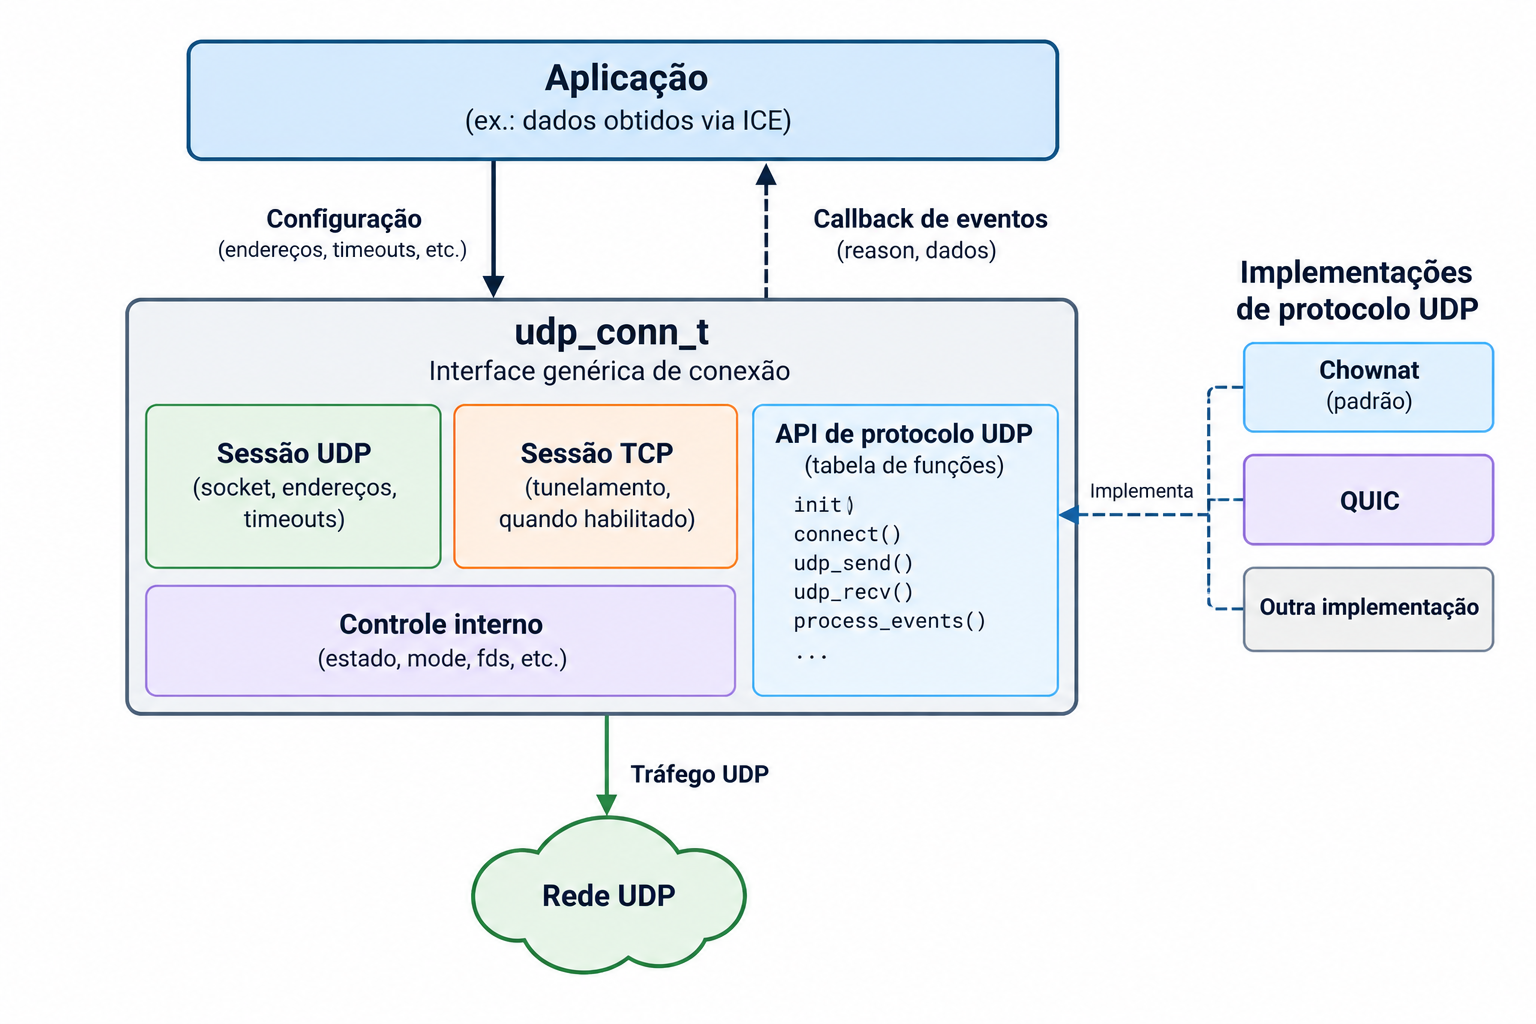
\includegraphics[width=0.8\textwidth]{fig/implementation/interface/udp_conn_diagram.png}
    \caption{Diagrama de blocos da interface genérica de conexão UDP udp\_conn\_t.}
    \label{fig:udp_conn_diagram}
\end{figure}

Além disso, esta interface genérica permite que o protocolo UDP que roda sobre ela funcione em dois modos: o modo cliente e o modo servidor. Cada um dos modos possui determinadas funções quando se está fazendo uso do tunelamento TCP. Esses mesmos comportamentos são os vistos na Seção~\ref{sec:chownat} e também serão abordados na próxima seção.

\subsubsection{Fluxo de conexão e hole punching}
\label{sec:interface_connection_flow_and_hole_punching}

A conexão utilizando esta interface se baseia em três operações diferentes; a ordem dessas operações é o que define se o processo está operando como cliente ou servidor. Portanto, dependendo do modo de operação da interface, essas operações são chamadas em uma ordem diferente. As operações utilizadas nesse processo são:

\begin{enumerate}
    \item \textbf{Bind TCP:} Responsável pelo vínculo da sessão TCP com o serviço local;
    \item \textbf{Hole Punching:} Realização de NAT traversal por UDP hole punching;
    \item \textbf{Conexão UDP:} Processo de conexão do protocolo em si, caso não integrado com \textit{hole punching}.
\end{enumerate}

Para entender essas diferenças, é importante retomar as etapas de conexão já descritas na Seção~\ref{sec:chownat_connection}. No modo cliente, aguarda-se uma conexão TCP realizada por um outro processo na própria máquina para o serviço desejado, enquanto, no modo servidor, apenas se espera por uma conexão UDP remota. Da mesma forma, após o recebimento da conexão UDP, o cliente inicia o \textit{hole punching}; já o servidor, após completar o \textit{hole punching}, conecta-se ao serviço TCP local. Isto implica uma ordem invertida entre essas duas operações, gerando o fluxo que pode ser visto na Figura~\ref{fig:udp_conn_connection_flow_diagram}:

\begin{figure}[ht]
    \centering
    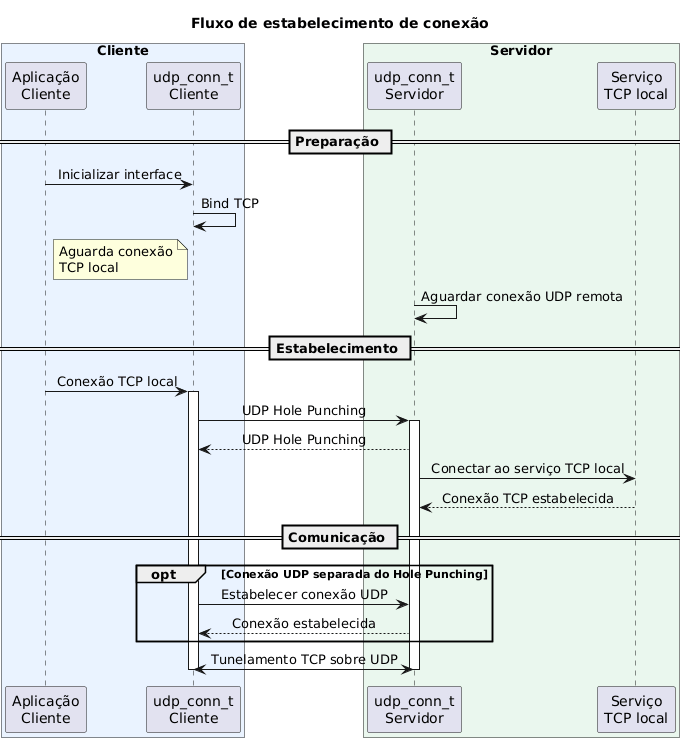
\includegraphics[width=0.8\textwidth]{fig/implementation/interface/udp_conn_connection_flow_diagram.png}
    \caption{Diagrama de tempo da interface de conexão UDP \texttt{udp\_conn\_t}.}
    \label{fig:udp_conn_connection_flow_diagram}
\end{figure}

Importante destacar que a implementação do protocolo UDP é responsável apenas pelas etapas que envolvem a comunicação externa com o outro \textit{peer}. Ou seja, as comunicações TCP internas ficam gerenciadas diretamente pela própria interface, abstraindo do protocolo a necessidade de conhecimento sobre o funcionamento do tunelamento.

\subsubsection{API e loop de eventos}
\label{sec:api_and_event_loop}

A API baseada em eventos é uma adição ao protocolo Chownat, permitindo um comportamento reativo, além de possibilitar o uso do protocolo sem que haja tunelamento TCP. Isso faz parte da extensão do protocolo Chownat implementada, descrita mais detalhadamente na Seção~\ref{sec:chownat_translation_extension}.

Existem dois níveis de recebimento de eventos. O primeiro são os eventos indicados pelo sistema operacional à própria interface, para indicar que um novo pacote foi recebido em uma determinada \textit{socket}. Isto é feito por meio da chamada de sistema \textit{select}, que permite a espera em um subconjunto de \textit{sockets}, gerando um evento para a interface e permitindo que ela continue executando a partir dessa chamada. Esta chamada já era utilizada no Chownat, e é um dos principais mecanismos que permite o \textit{hole punching} a partir do envio de pacotes \textit{keep-alive}, como visto na Listagem~\ref{lst:select_pseudocode}.

\begin{lstlisting}[caption={Pseudocódigo do loop de eventos da interface}, label={lst:select_pseudocode}]
    while (true)
        ret = select(sockets, ..., timeout)
        if (ret == TIMEOUT_EXCEEDED)
            send_keep_alive()
        else
            handle_sockets()
\end{lstlisting}

O outro nível são os eventos recebidos pela própria aplicação. Estes eventos são determinados por cada implementação de protocolo, dado que cada uma pode possuir diferentes tipos de eventos, podendo ser o recebimento de determinada mensagem, de determinado erro, início e fim de conexão, etc. Isso permite que a aplicação possa interferir no fluxo de conexão em determinados momentos, a partir da API pública da interface, que inclui as seguintes ações:

\begin{itemize}
    \item \textbf{udp\_conn\_send:} Enviar mensagem;
    \item \textbf{udp\_conn\_recv:} Esperar recebimento de mensagem;
    \item \textbf{udp\_conn\_disconnect:} Finalizar conexão.
\end{itemize}

Além desta API pública, existem ainda as funções de criação de conexão, que não são permitidas dentro do \textit{loop} de eventos, sendo elas:

\begin{itemize}
    \item \textbf{udp\_conn\_init:} Inicializa a interface com determinada implementação;
    \item \textbf{udp\_connection:} Inicializa a conexão. É o próprio \textit{loop} de eventos; ao entrar nessa função, só sai dela se a conexão for finalizada;
    \item \textbf{udp\_conn\_deinit:} Desinicializa a interface.
\end{itemize}

\subsubsection{Tunelamento TCP}

O tunelamento TCP é um dos principais atributos da arquitetura do Chownat, permitindo a conectividade entre \textit{peers} e o reuso de serviços já implementados sobre TCP, com menor \textit{overhead} de comunicação, modularidade dos serviços (pois desacopla, de forma indireta, o protocolo de transporte) e facilidade de migração de serviços baseados em TCP para UDP. Essa facilidade de migração representa uma característica relevante para a proposta deste trabalho, considerando a ampla utilização de protocolos de aplicação baseados em TCP e em arquiteturas cliente-servidor no contexto da Internet das Coisas (IoT), como HTTP e MQTT. Dessa forma, a solução proposta busca facilitar a adoção de uma arquitetura \textit{peer-to-peer} por aplicações existentes, reduzindo a necessidade de modificações nos serviços originalmente desenvolvidos para comunicação sobre TCP.

A interface permite o uso de técnicas de tunelamento de forma transparente à implementação do protocolo, mantendo-o como um atributo opcional para a aplicação que fará uso da interface. Como visto anteriormente na Seção~\ref{sec:chownat}, a conexão TCP ocorre apenas de forma local, e os pacotes produzidos pelo serviço são enviados à interface por meio de uma \textit{socket} TCP vinculada ao serviço em execução, permitindo que segmentos de controle TCP (como ACKs, FIN, SYN) existam apenas localmente, mantendo, para a conexão remota externa, apenas o envio de dados do serviço de aplicação (HTTP, SSH, etc.). Entretanto o protocolo UDP pode transmitir seus próprios pacotes de controle. Quando a aplicação envia uma mensagem para a \textit{socket} vinculada, o \textit{loop} de eventos da interface (visto na Seção~\ref{sec:api_and_event_loop}) é ativado, avisando-a do recebimento da mensagem em uma das \textit{sockets}. É então analisado em qual \textit{socket} o pacote foi recebido: caso seja na \textit{socket} TCP, os dados do pacote são coletados e enviados através da implementação UDP. Ao receber um pacote do \textit{loop} de eventos da interface, caso ele seja UDP, basta retornar os dados à interface, que será responsável por verificar a existência de tunelamento e redirecionar os dados recebidos para a \textit{socket} TCP local, permitindo uma resposta à aplicação. Este fluxo completo pode ser visto na Figura~\ref{fig:udp_conn_tcp_tunneling_diagram}.

\begin{figure}[ht]
    \centering
    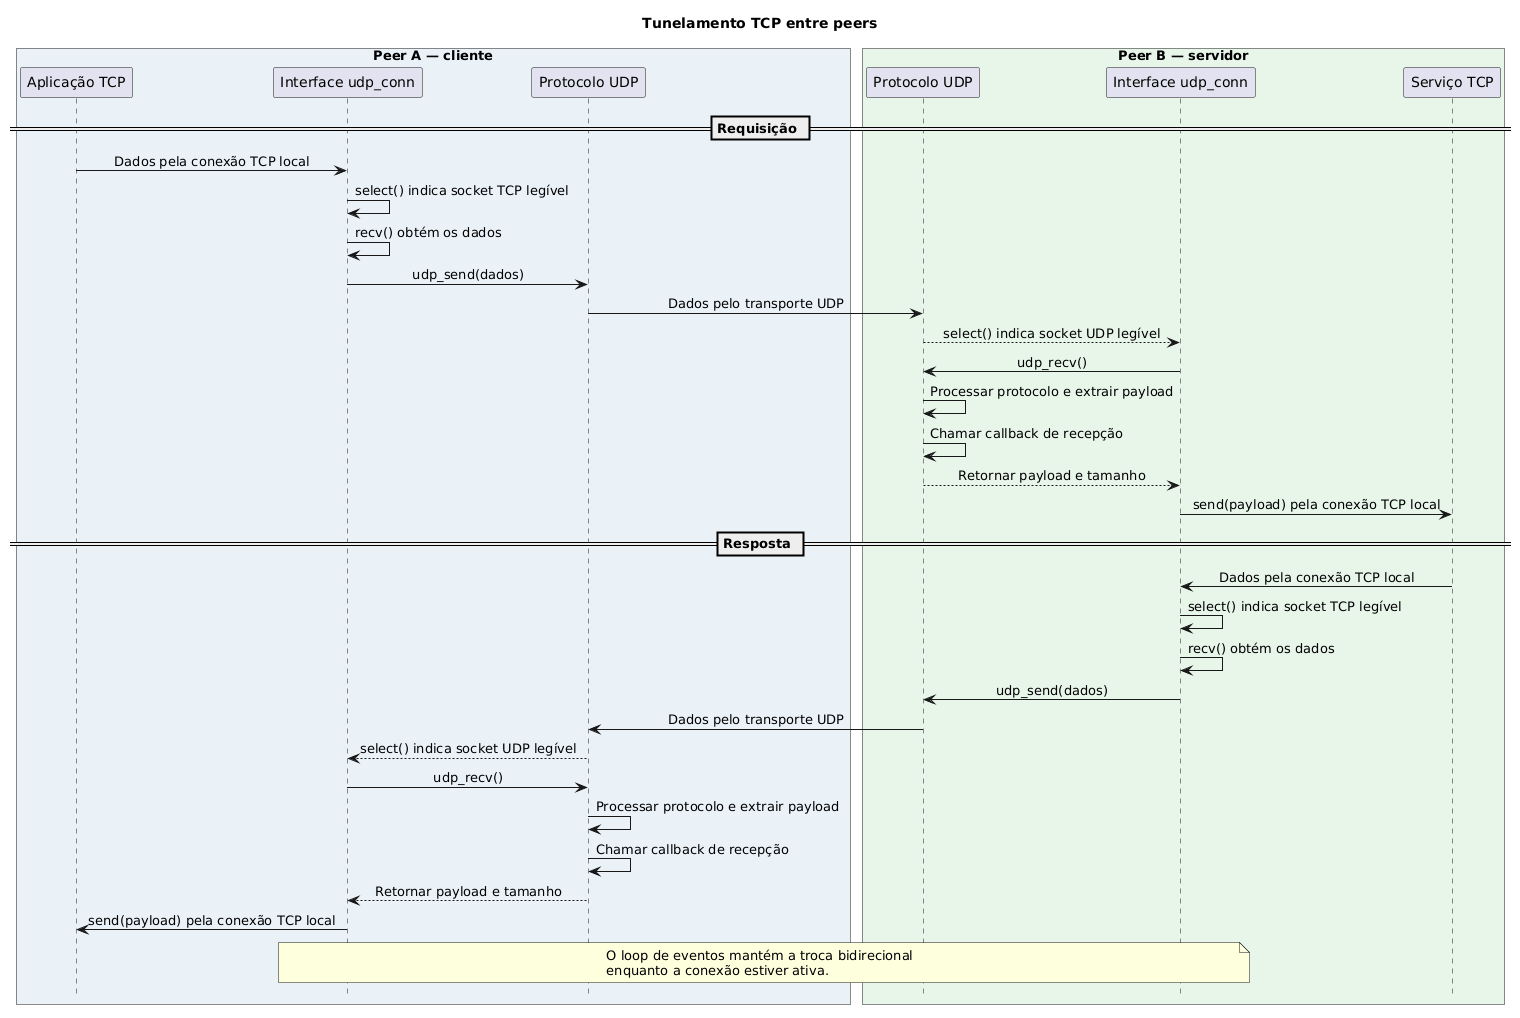
\includegraphics[width=1.0\textwidth]{fig/implementation/interface/udp_conn_tcp_tunneling_diagram.png}
    \caption{Diagrama de tempo de uma requisição TCP tunelada por UDP utilizando a interface udp\_conn\_t.}
    \label{fig:udp_conn_tcp_tunneling_diagram}
\end{figure}

No cenário considerado, a aplicação integrada ao túnel executa no próprio gateway. Ela utiliza uma conexão TCP local para entregar e receber os dados transportados entre os hosts. A obtenção desses dados a partir de sensores, assim como seu encaminhamento a atuadores locais, pertence à aplicação do gateway e não é implementada pelo túnel. Nos experimentos, essas funções são abstraídas por aplicações locais de geração e recepção de mensagens.

\subsection{Tradução e Extensão do Protocolo Chownat}
\label{sec:chownat_translation_extension}

O protocolo Chownat, como visto anteriormente, é nativo em Perl, disponível em \citep{kamkar2004chownatv07}. Durante o projeto da Datacom descrito no início desta seção, foi escolhido o uso deste protocolo, dado que ele era capaz de suprir as necessidades momentâneas para compreensão e aplicação de técnicas de NAT traversal, assim como pela existência do \textit{hole punching} de forma nativa ao protocolo, além do tunelamento TCP, que permitia o tráfego TCP necessário para as aplicações HTTP do projeto.

Durante o projeto com a Datacom, foi feita uma tradução do protocolo para C e Dart, de forma a manter sua forma nativa de funcionamento, sem extensões e sem modificações, apenas replicação da funcionalidade. Entretanto, a tradução não havia sido feita de forma completa, e possuía diversas limitações, principalmente associadas às etapas de criação, reinício e finalização de conexões. Além disso, por conta do propósito inicial do Chownat possuir apenas tunelamento TCP, não era possível utilizar uma comunicação apenas com UDP.

O objetivo do desenvolvimento de extensões e modificações no próprio Chownat, apesar de este não ser o objetivo principal do trabalho, foi a realização de testes de funcionamento e a generalização da própria interface (vista na Seção~\ref{sec:hole_punching_interface}) para protocolos posteriores, como o QUIC. Portanto, o valor desse desenvolvimento está associado muito mais à garantia de funcionamento do que à real sugestão de uso deste protocolo para qualquer tipo de aplicação posterior, dadas as diversas limitações, como a falta de garantia dos requisitos de dependabilidade (citados na introdução deste trabalho) cruciais na transmissão de dados da comunicação IoT.

\subsubsection{Limitações do Chownat e extensões desenvolvidas}
\label{sec:chownat_limitations}

O protocolo Chownat possui diversas limitações, principalmente associadas ao seu objetivo original. No momento de seu desenvolvimento (2004) \citep{kamkar2004chownat}, técnicas de NAT traversal ainda estavam sendo exploradas, e o uso de arquiteturas de rede P2P ainda era mal visto, devido ao seu histórico de uso em contextos de pirataria. Portanto, o objetivo principal do Chownat não parece ter sido pensado para o uso contínuo em um dispositivo, mas sim principalmente para provar o funcionamento de técnicas de \textit{hole punching} sobre dispositivos NAT.

Dado que a interface genérica apresentada na Seção~\ref{sec:hole_punching_interface} foi baseada inicialmente no protocolo Chownat, foram propostos alguns mecanismos para generalizar a interface e viabilizar seu uso completo por outros protocolos, o que implica que o próprio Chownat também passa a se beneficiar dessas mudanças. Nem todas as limitações foram solucionadas, principalmente por serem específicas do protocolo, como suas próprias garantias de dependabilidade; ainda assim, parte delas foi resolvida para permitir a realização de testes sobre os recursos da interface. As principais limitações, e o tratamento dado a cada uma, são:

\begin{itemize}
    \item \textbf{Conexão suporta apenas o envio de 256 pacotes:} existe apenas um único byte de representação de identificador de pacote, portanto existem apenas valores possíveis entre 0 e $2^8-1$ para os identificadores. Optou-se por manter o mesmo cabeçalho do Chownat (Seção~\ref{sec:chownat_protocol}), reinicializando a contagem de pacotes ao atingir o limite; perdas de mais de 256 pacotes consecutivos ainda geram comportamento indefinido, mas essa solução foi preferida a estender o campo para 2 bytes, preservando o formato original do pacote;
    \item \textbf{Apenas permite comunicação de dados TCP:} o protocolo Chownat funciona apenas tunelando TCP, não sendo possível o envio nativo de dados UDP sem a existência do tunelamento. Com a criação da interface genérica, o tunelamento TCP passou a ser opcional por conexão, permitindo que a aplicação envie dados nativamente, sem depender de uma conexão TCP externa;
    \item \textbf{Permite apenas uma conexão por aplicação:} ao finalizar a única conexão TCP suportada, o protocolo original entrava em \textit{loop} infinito. Isso foi resolvido com a implementação de um \textit{3-way-handshake} de desconexão, com número máximo de tentativas configurável por conexão, permitindo que, ao finalizar uma conexão TCP, a conexão Chownat também seja finalizada e uma nova conexão possa ser inicializada;
    \item \textbf{Hole punching exige tradução de porta com ``mapeamento espelhado'':} o \textit{hole punching} do Chownat depende de o mapeamento das portas seguir uma regra específica, traduzindo-as exatamente para a porta de origem vinculada pela \textit{socket} que enviará o pacote UDP. Na prática, alguns NATs assumem esse comportamento, como o NAT simulado pelo PatchBay \citep{patchbay} no modo \textit{Moderate}, mas trata-se de um caso particular, e não de uma regra geral entre implementações de NAT. Este problema foi posteriormente resolvido com a integração da biblioteca ICE, descrita na Seção~\ref{sec:ice_library};
    \item \textbf{Sem garantias de dependabilidade:} o protocolo não possui qualquer garantia de confiabilidade, integridade, autenticidade e segurança. Esse problema não foi resolvido, dado que o objetivo final é o uso do protocolo QUIC, que oferece nativamente mecanismos de entrega confiável e proteção criptográficare, mantendo-se, portanto, a simplicidade do Chownat para fins exclusivos de teste.
\end{itemize}

Em síntese, as extensões desenvolvidas não transformam o Chownat em um protocolo pronto para uso em produção, sua limitação mais fundamental, a ausência de garantias de dependabilidade, foi deliberadamente deixada sem solução. O valor desse trabalho de extensão está em ter viabilizado um protocolo funcional e já conhecido como base de testes para a interface genérica proposta neste trabalho, permitindo validar empiricamente as técnicas de \textit{hole punching} antes de aplicá-las a um protocolo com garantias mais robustas, como o QUIC.

\subsection{Uso da Biblioteca OpenSSL para QUIC Hole Punching}
\label{sec:ossl_quic_for_hole_punching}

Dada a complexidade do protocolo QUIC, como visto anteriormente no Capítulo~\ref{chap:quic}, optou-se por utilizar uma biblioteca para realizar a comunicação entre \textit{peers} utilizando este protocolo. Além disso, o protocolo possui diversas características associadas à segurança, o que contribui como outro fator contrário à implementação própria, de forma a evitar riscos de segurança associados a qualquer falha de implementação.

Dado o objetivo de utilizar uma arquitetura baseada no protocolo Chownat, optou-se por não utilizar uma implementação já existente de QUIC hole punching, pois estas seguem abordagens diferentes, como a realização de alterações no próprio protocolo QUIC, a exemplo da segunda proposta de \citep{draft-seemann-quic-nat-traversal}. Portanto, o objetivo foi utilizar uma biblioteca já implementada e bem estabelecida para a realização da primeira alternativa de QUIC \textit{hole punching} proposta por \citep{draft-seemann-quic-nat-traversal}, que se resume em realizar o \textit{hole punching} previamente, via ICE ou outro método equivalente, seguido da transição para a conexão QUIC sobre o caminho já estabelecido.

Para a implementação do protocolo QUIC, optou-se pela utilização da biblioteca OpenSSL, um projeto de código aberto consolidado no desenvolvimento de soluções criptográficas e protocolos de comunicação segura. A partir da versão 3.2, disponibilizada em novembro de 2023 (como visto por \citep{openssl_quic}), a OpenSSL passou a oferecer suporte nativo a conexões QUIC no lado cliente, posteriormente expandido para o lado servidor na versão 3.5. A escolha dessa biblioteca fundamenta-se na manutenção ativa do projeto, na disponibilidade de documentação oficial e na integração do protocolo QUIC à API SSL já existente, permitindo reutilizar abstrações e mecanismos de comunicação disponibilizados pela biblioteca. Além disso, a biblioteca OpenSSL permite o uso de uma \textit{socket} externa, possibilitando reutilizar uma \textit{socket} que, por exemplo, já tenha passado por \textit{hole punching}, mantendo o caminho aberto para a conexão QUIC, o que é um pré-requisito para o uso da abordagem baseada na arquitetura Chownat com a primeira alternativa proposta por \citep{draft-seemann-quic-nat-traversal}, dado que não há alterações na implementação original do protocolo.

A plataforma de execução considerada é o \textit{host} que representa o \textit{gateway}. A escolha das bibliotecas prioriza os recursos necessários à integração e à avaliação do transporte. O trabalho não estabelece requisitos mínimos de execução nem caracteriza o consumo dessas dependências em dispositivos IoT com recursos limitados.

\subsubsection{Configuração e conexão do protocolo QUIC}

Para a configuração, a implementação do protocolo sobre a interface expõe parte da API da OpenSSL; portanto, nem todos os recursos disponibilizados estão acessíveis, e a implementação funciona mais como um \textit{wrapper}, adicionando algumas configurações à API que simplificam o uso para o usuário. Esta implementação \textit{wrapper} foi denominada com o nome ``ossl\_quic''. O usuário poderá configurar, tanto para o cliente quanto para o servidor, as suítes de criptografia disponibilizadas pela OpenSSL para o TLS 1.3, que é o único protocolo de criptografia disponível para a comunicação QUIC.

A implementação da OpenSSL é baseada em contextos, e cada contexto permite uma série de configurações diferentes. As configurações para cliente e servidor diferem, principalmente por não estar sendo utilizada a variante de mTLS (\textit{Mutual Transport Layer Security}), responsável pela garantia de autenticidade tanto do servidor quanto do cliente. Nos experimentos, foi utilizado um certificado autoassinado e a validação do certificado pelo cliente foi desabilitada. Essa configuração permite o estabelecimento da conexão cifrada, mas não verifica a identidade do servidor remoto. Seu uso foi restrito aos testes e é desaconselhado em ambientes de produção. Em ambientes de produção, a validação do certificado deve estar habilitada, com uma configuração de confiança adequada para verificar a identidade do servidor remoto.

Além disso, apesar de não ter sido abordado no Capítulo~\ref{chap:quic}, o QUIC também permite a configuração de um protocolo de aplicação a partir da ALPN (\textit{Application Layer Protocol Negotiation}), a fim de definir um protocolo acordado para uso durante a negociação da conexão. Neste caso, essa configuração não é estritamente necessária, pois o objetivo é apenas o transporte de dados genéricos, não associados a um protocolo específico; para isso, utiliza-se apenas um nome arbitrário, escolhido como sendo ``osslquic''.

Assim como no Chownat, esta etapa inicial inicializa a \textit{socket} UDP, vinculando-a a um endereço específico, da mesma forma descrita na Seção~\ref{sec:chownat}. O diagrama de tempo desta configuração pode ser visto na Figura~\ref{fig:ossl_quic_configuration}.

\begin{figure}[ht]
    \centering
    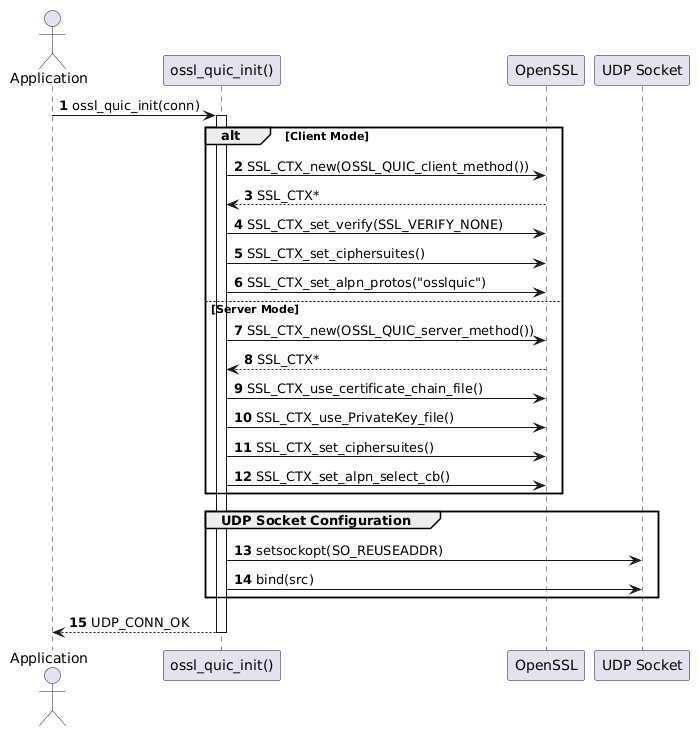
\includegraphics[width=0.8\textwidth]{fig/implementation/ossl_quic/ossl_quic_configuration_time_diagram.png}
    \caption{Diagrama de tempo da configuração do QUIC da OpenSSL sobre a interface.}
    \label{fig:ossl_quic_configuration}
\end{figure}

\subsubsection{Processo de hole punching e conexão}

O processo de \textit{hole punching} da implementação ``ossl\_quic'' segue o mesmo padrão visto no Chownat: o objetivo central é a realização do \textit{hole punching} de forma prévia à conexão QUIC, implementando assim, de forma parcial, a primeira proposta descrita por \citep{draft-seemann-quic-nat-traversal}. Na prática, este \textit{hole punching} pode ser realizado utilizando o próprio ICE, como descrito na Seção~\ref{sec:ice_library}.

Após a realização do \textit{hole punching} por si só, inicia-se a conexão QUIC. Isto implica a implementação da etapa opcional de conexão UDP, descrita na Seção~\ref{sec:interface_connection_flow_and_hole_punching} e ilustrada na Figura~\ref{fig:udp_conn_connection_flow_diagram}. Para a realização desta operação, é primeiro necessário executar uma operação interna da implementação, chamada por este trabalho de \textit{pre connect}. Além disso, é relevante relembrar que não é necessário realizar o descarte de pacotes manualmente, pois, como visto na Seção~\ref{sec:quic_long_header_packets}, que se baseia em \citep{rfc9000}, pacotes \texttt{Initial} recebidos pela \textit{engine} do QUIC que possuam tamanho menor que 1200 bytes já são descartados automaticamente por ela.

A \textit{pre connect} é uma operação realizada antes da conexão, como o próprio nome sugere, sendo responsável por criar uma nova conexão SSL (nome dado às conexões da OpenSSL), posteriormente utilizada para realizar a conexão QUIC. Esta operação executa três ações principais: cria a conexão (ou \textit{listener}, no caso do servidor); inicializa cada um desses objetos em seu devido estado; e vincula o FD (\textit{file descriptor}) correspondente, configurando a conexão do cliente como cliente e a do servidor como \textit{listener}. Além disso, no lado do cliente, é chamada a função \texttt{connect} da POSIX, responsável por vincular uma \textit{socket} UDP a um endereço remoto, sem necessariamente realizar uma conexão (diferentemente do que ocorreria com TCP). Já no lado do servidor, a \textit{socket} é configurada inicialmente como bloqueante, para que o servidor aguarde pela própria conexão QUIC.

Durante a conexão, o QUIC no modo servidor apenas aguarda, com um \texttt{accept}, até receber uma conexão externa, enquanto no modo cliente é iniciada uma operação de conexão utilizando a biblioteca OpenSSL. Esta operação de conexão realiza as etapas descritas na Seção~\ref{sec:quic_connection_steps}.

\subsubsection{Gerência da conexão}

A gerência da conexão ocorre da mesma forma que a vista no Chownat, na Seção~\ref{sec:chownat}, através do uso de \textit{keep-alives} e do envio de mensagens por chamadas \texttt{send} e \texttt{recv}, além da gerência do tunelamento TCP já discutida anteriormente. Entretanto, por conta de a \textit{engine} QUIC provida pela OpenSSL ser mais elaborada do que um protocolo simples como o Chownat, foi necessária uma extensão da interface descrita na Seção~\ref{sec:hole_punching_interface}, de forma a suportar possíveis comportamentos da implementação do protocolo. Esta extensão da interface incluiu o processamento de possíveis eventos, em conjunto com o processamento de possíveis dados pendentes do protocolo.

O processamento de eventos é necessário dado que a interface é \textit{threadless}, como visto anteriormente na Seção~\ref{sec:hole_punching_interface}. Isto implica que eventos assíncronos, como \textit{timeouts} ou o tratamento do recebimento e envio de pacotes de controle, precisam ser processados explicitamente pela própria interface. Como descrito por \citep{openssl_ssl_handle_events}, isso não seria necessário caso a biblioteca estivesse configurada para o modo de assistência por \textit{threads}, já que, nesse modo, a \textit{thread} de controle da biblioteca seria periodicamente responsável pelo tratamento desses eventos. Estes eventos também são gerenciados nas chamadas de \textit{read} e \textit{write}, que operam em modo bloqueante apenas dur103ante a etapa de conexão, sendo não bloqueantes em todos os demais momentos. Importante destacar que, mesmo no modo bloqueante, ainda é necessário o tratamento de eventos quando as chamadas de \textit{read} e \textit{write} ocorrem apenas após longos períodos de tempo.

O processamento de dados pendentes, por sua vez, decorre de um comportamento específico da biblioteca OpenSSL. Ao receber um conjunto de pacotes QUIC, seja através do processamento de eventos, seja a partir de operações de \textit{read}, a biblioteca armazena esses pacotes em um \textit{buffer} interno de sua própria implementação, deixando dados pendentes de leitura que, no entanto, não são mais lidos diretamente da \textit{socket}, e sim da própria biblioteca. Na abordagem original do Chownat, a espera por dados dependia inteiramente da existência de dados na \textit{socket}, verificada pelo \textit{loop} de eventos. Ao utilizar a biblioteca QUIC, entretanto, essa mesma lógica de espera na \textit{socket} passa a ser insuficiente: a \textit{socket} é considerada vazia assim que a OpenSSL a esvazia internamente, mesmo que outros pacotes tenham chegado e sido armazenados no \textit{buffer} interno da biblioteca, ainda pendentes de processamento. Por esse motivo, também se faz necessário o processamento desses dados pendentes na própria implementação interna da interface.

Além disso, ao ser adicionado o processamento de eventos, uma segunda dependência temporal passa a existir na interface. Inicialmente, a única dependência temporal era o \textit{timeout} de atividade nas \textit{sockets}, controlado pela chamada de sistema \textit{select}; com a extensão, passa a existir também o \textit{timeout} para a ocorrência de eventos internos, gerenciado pela própria implementação da OpenSSL. Isto implica que o tempo de espera do \textit{select} pode precisar ser mais curto, em função da necessidade de tratar um evento interno do protocolo antes do próximo \textit{keep-alive}.

A forma como isso foi resolvido consiste em manter um ponto de referência de inatividade, atualizado sempre que ocorre atividade na \textit{socket}. A cada iteração, os dois \textit{timeouts} são comparados, e o menor entre eles é utilizado como tempo de espera do \textit{select}. Ao ocorrer um \textit{timeout} do \textit{select}, verifica-se se o ponto de inatividade já foi atingido ou ultrapassado: em caso afirmativo, o \textit{timeout} ocorreu por inatividade, e um \textit{keep-alive} é enviado para manter o mapeamento do NAT. Caso contrário, o \textit{timeout} foi causado pelo \textit{timeout} interno de eventos, mais curto; nesse caso, o \textit{loop} retorna ao início e processa os eventos e pacotes pendentes antes de aguardar novamente pelo próximo pacote no \textit{select}.

Desta forma, o fluxo visto previamente na Figura~\ref{fig:udp_conn_tcp_tunneling_diagram} recebe algumas alterações, de forma a se manter portável para bibliotecas com certos requisitos não exigidos nem tratados anteriormente pelo Chownat, devido à sua simplicidade. Isto resulta em um fluxo com os passos vistos na Figura~\ref{fig:udp_conn_additional_methods}.

\begin{figure}[!ht]
    \centering
    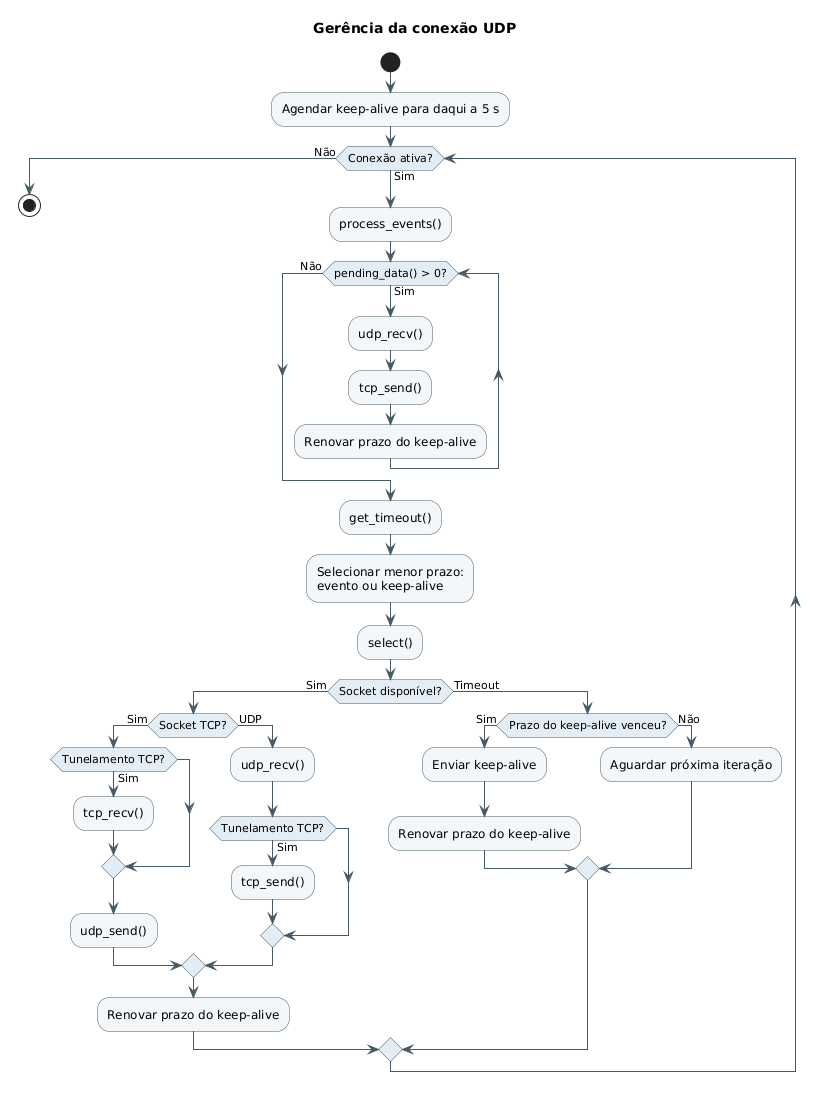
\includegraphics[width=0.8\textwidth]{fig/implementation/ossl_quic/new_udp_conn_diagram.png}
    \caption{Diagrama de atividades do fluxo atualizado da interface \texttt{udp\_conn\_t}.}
    \label{fig:udp_conn_additional_methods}
\end{figure}

\section{Uso da Biblioteca libnice para a Integração do Protocolo ICE}
\label{sec:ice_library}

Como visto anteriormente na Seção~\ref{sec:ice}, o protocolo ICE é o protocolo responsável pela descoberta prévia dos endereços IP de cada \textit{peer} que deseja realizar uma comunicação P2P a partir de técnicas de NAT traversal. A implementação descrita até então na Seção~\ref{sec:hole_punching_protocols} herda do protocolo Chownat a dependência do conhecimento prévio desses endereços pelo \textit{peer}. Isto implica a dependência chamada por este trabalho de ``mapeamento espelhado'', também descrita na Seção~\ref{sec:chownat_limitations}. Como forma de propor uma solução genérica para este problema, tanto para o próprio Chownat quanto para protocolos que herdam a interface genérica \texttt{udp\_conn} descrita na Seção~\ref{sec:hole_punching_interface}, foi criada uma nova interface de transporte, responsável pela gerência da \textit{socket} UDP da conexão, que permite à aplicação escolher o modelo de protocolo de transporte, suportando tanto a abordagem legada descrita na Seção~\ref{sec:hole_punching_interface} quanto a nova abordagem descrita nesta seção, utilizando ICE.

Durante a busca entre as principais bibliotecas de ICE, foi escolhida a \texttt{libnice}. Esta escolha se deve principalmente à praticidade de integração, devido a esta já possuir uma API baseada em eventos utilizando a biblioteca \texttt{GLib}, além de prover um controle completo sobre os protocolos STUN e TURN, mantendo-os de forma abstraída da implementação. Além disso, a \texttt{libnice} é implementada em C, o que facilita a integração direta com sua API. Outro ponto importante na escolha da biblioteca foi sua maturidade e validação, além de sua interoperabilidade com a Google WebRTC Library \citep{WebRTCOrg}, principal biblioteca de implementação de WebRTC utilizada na maioria dos navegadores, como apontado pela própria \texttt{libnice} em \citep{libnice}, o que implica também uma implementação que segue fielmente o RFC8445 \citep{rfc8445}, facilitando a integração com outros serviços para teste, como a própria biblioteca \texttt{coturn} \citep{coturn}.

\subsection{Interface de gerência de sockets}

Diferentemente da abordagem que vinha sendo utilizada, que permitia controle completo da \textit{socket} UDP usada no transporte dos pacotes, a \texttt{libnice} não expõe diretamente a sua \textit{socket}, impossibilitando a manutenção da mesma abordagem. Isto ocorre devido a necessidade da gerência de possíveis pacotes de \textit{keep-alive} da conexão ou até mesmo tunelamento dos dados até um servidor TURN como visto pela figura \ref{fig:turn_quic_tcp_tunneling}

\begin{figure}[ht]
    \centering
    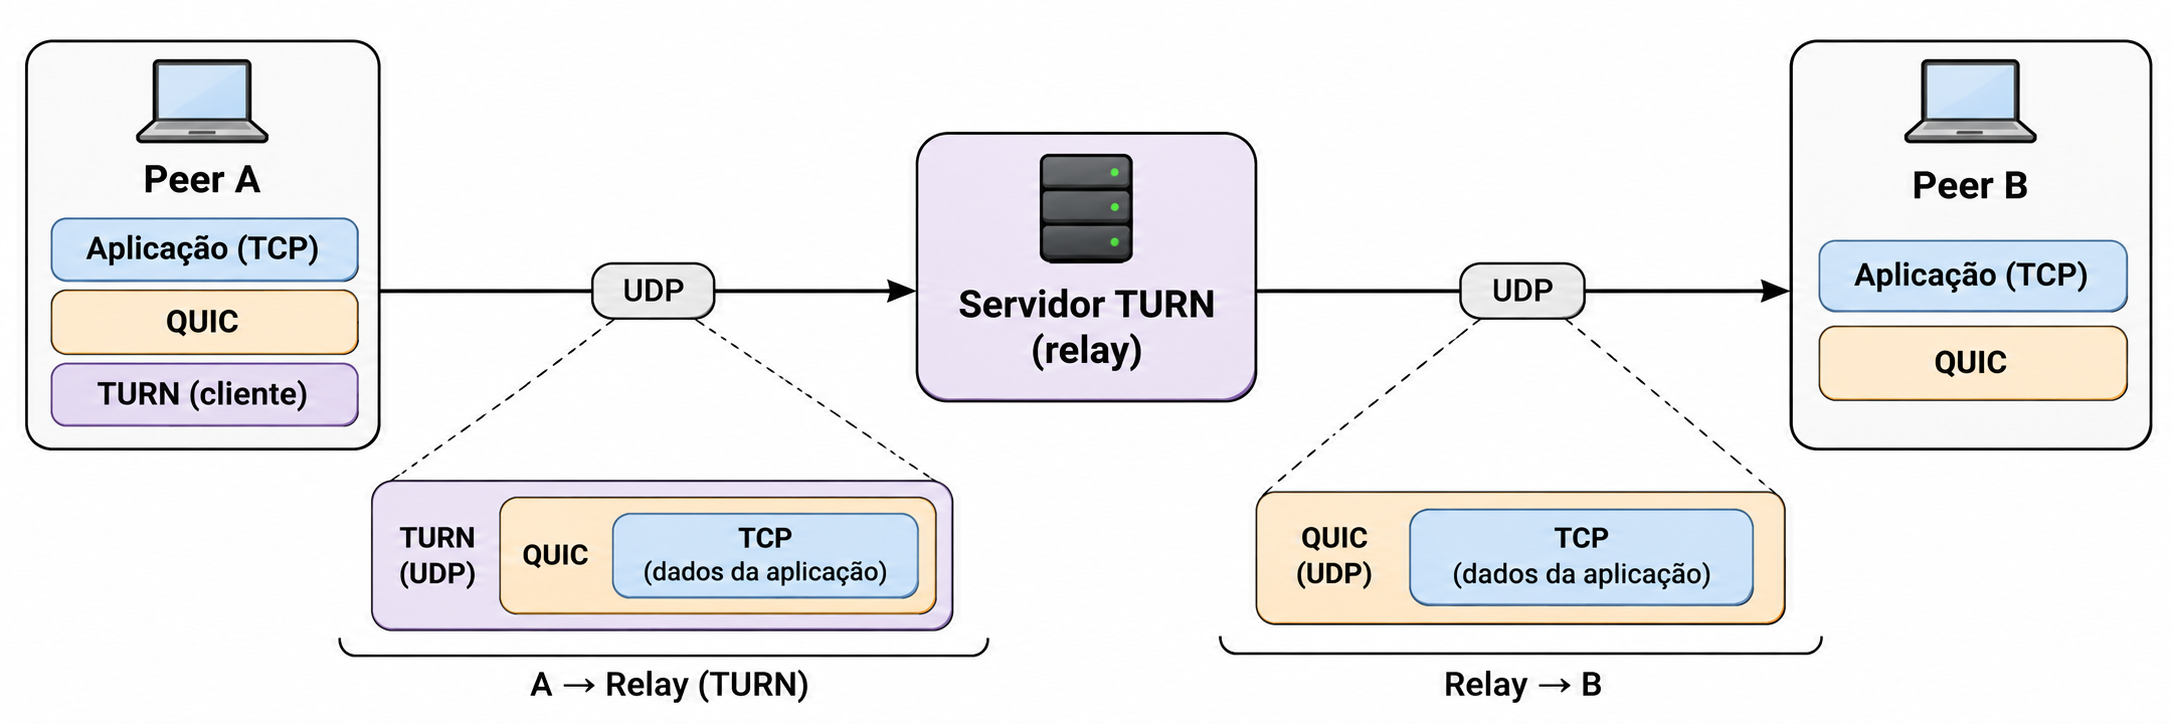
\includegraphics[width=0.8\textwidth]{fig/implementation/libnice/turn_quic_tcp_tunneling.png}
    \caption{Representação de transimssão de pacote TCP tunelados sobre QUIC sendo tunelados por TURN até o servidor \textit{relay}.}
    \label{fig:turn_quic_tcp_tunneling}
\end{figure}


Até então, chamadas POSIX eram feitas passando diretamente a \textit{socket} utilizada (\texttt{sendto}, \texttt{recvfrom}, etc.). Portanto, para a adequação e manutenção dessa mesma estrutura, foi criada uma camada fina responsável por abstrair a existência da \textit{socket} UDP, permitindo que as chamadas fossem feitas sem a necessidade de acesso direto a ela. Esta camada fina é uma interface que define um contrato a ser implementado por determinadas soluções, chamada de \texttt{udp\_transport\_t}. Isto permite que implementações específicas, como o uso da \texttt{libnice}, implementem o contrato desta interface, mantendo os detalhes de sua gerência de \textit{socket} opacos, abstraídos dos usuários desta mesma camada, que, neste caso, é a própria interface \texttt{udp\_conn} e suas respectivas implementações. Além disso, a existência desta camada permite manter a solução legada, que gerencia \textit{sockets} diretamente. Essa estrutura, se representada por um diagrama, permite a flexibilidade demonstrada na Figura~\ref{fig:udp_transport_interface}, onde a solução legada foi chamada de ``Direct UDP'' e a nova solução é a solução ICE.

\begin{figure}[ht]
    \centering
    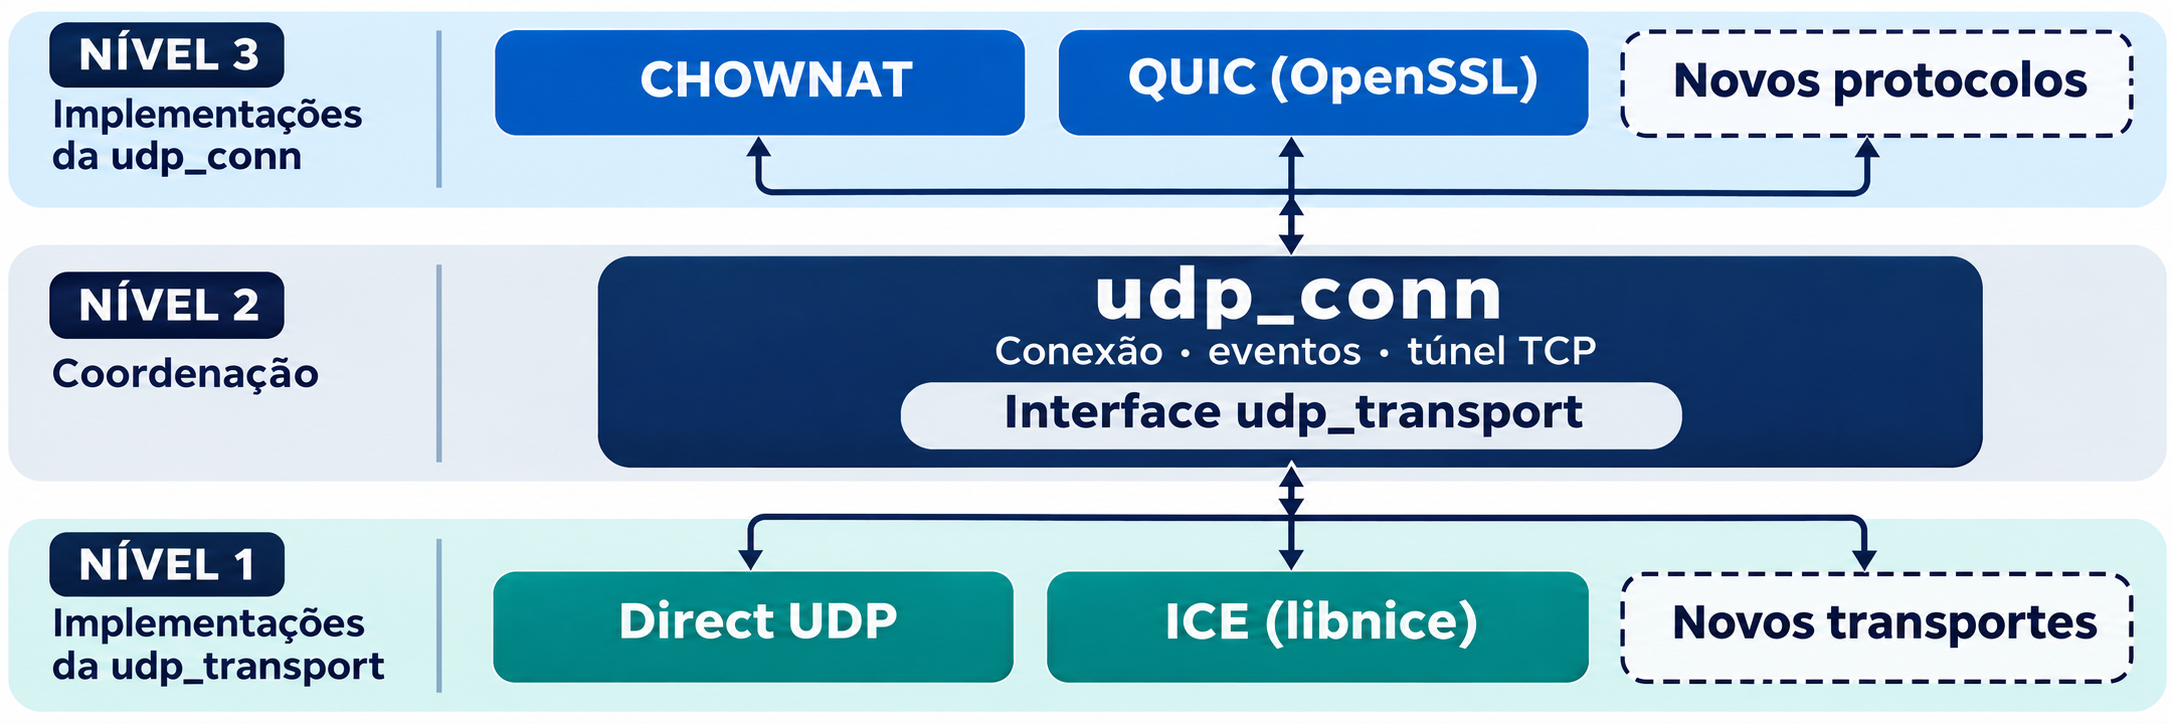
\includegraphics[width=0.8\textwidth]{fig/implementation/interface/udp_transport_flexibility.png}
    \caption{Diagrama de estrutura pós-adesão da interface \texttt{udp\_transport\_t}.}
    \label{fig:udp_transport_interface}
\end{figure}

\subsection{QUIC da OpenSSL com BIO}

Diferentemente da implementação do protocolo Chownat, em que as chamadas de manipulação de conexão e dados eram feitas através das funções da POSIX, a conexão e o transporte do protocolo QUIC da OpenSSL abstraem o uso dessas funções, fornecendo versões próprias e permitindo apenas o envio através da \textit{socket} escolhida. Portanto, não é possível simplesmente alternar sua implementação para chamar uma função de \texttt{udp\_transport}; do contrário, o \texttt{udp\_transport} precisaria conhecer a implementação QUIC, o que quebraria o contrato e inviabilizaria o isolamento da interface \texttt{udp\_transport} sem conhecimento do protocolo de transporte utilizado.

Entretanto, a OpenSSL fornece um recurso denominado BIO (\textit{Basic Input/Output}). Um BIO é uma abstração, ou pode também ser visto como outra interface, que permite abstrair o tipo de entrada e saída utilizado (arquivo, \textit{socket}, \textit{buffer}, etc.), permitindo que uma implementação específica defina um contrato próprio para o tratamento dos dados recebidos por esse BIO. Na prática, toda implementação da OpenSSL cria um BIO internamente, o que também permite que, caso outra implementação queira utilizar um contrato diferente do padrão da OpenSSL, baste implementar esse contrato. 

Esta solução resolve exatamente o problema abordado anteriormente, pois desta forma, o contrato de uma nova conexão BIO pode chamar a implementação de \texttt{udp\_transport}, abstraindo da camada acima o conhecimento sobre o protocolo de transporte utilizado. O fluxo pode ser visto na Figura~\ref{fig:openssl_quic_bio_update}.

\begin{figure}[ht]
    \centering
    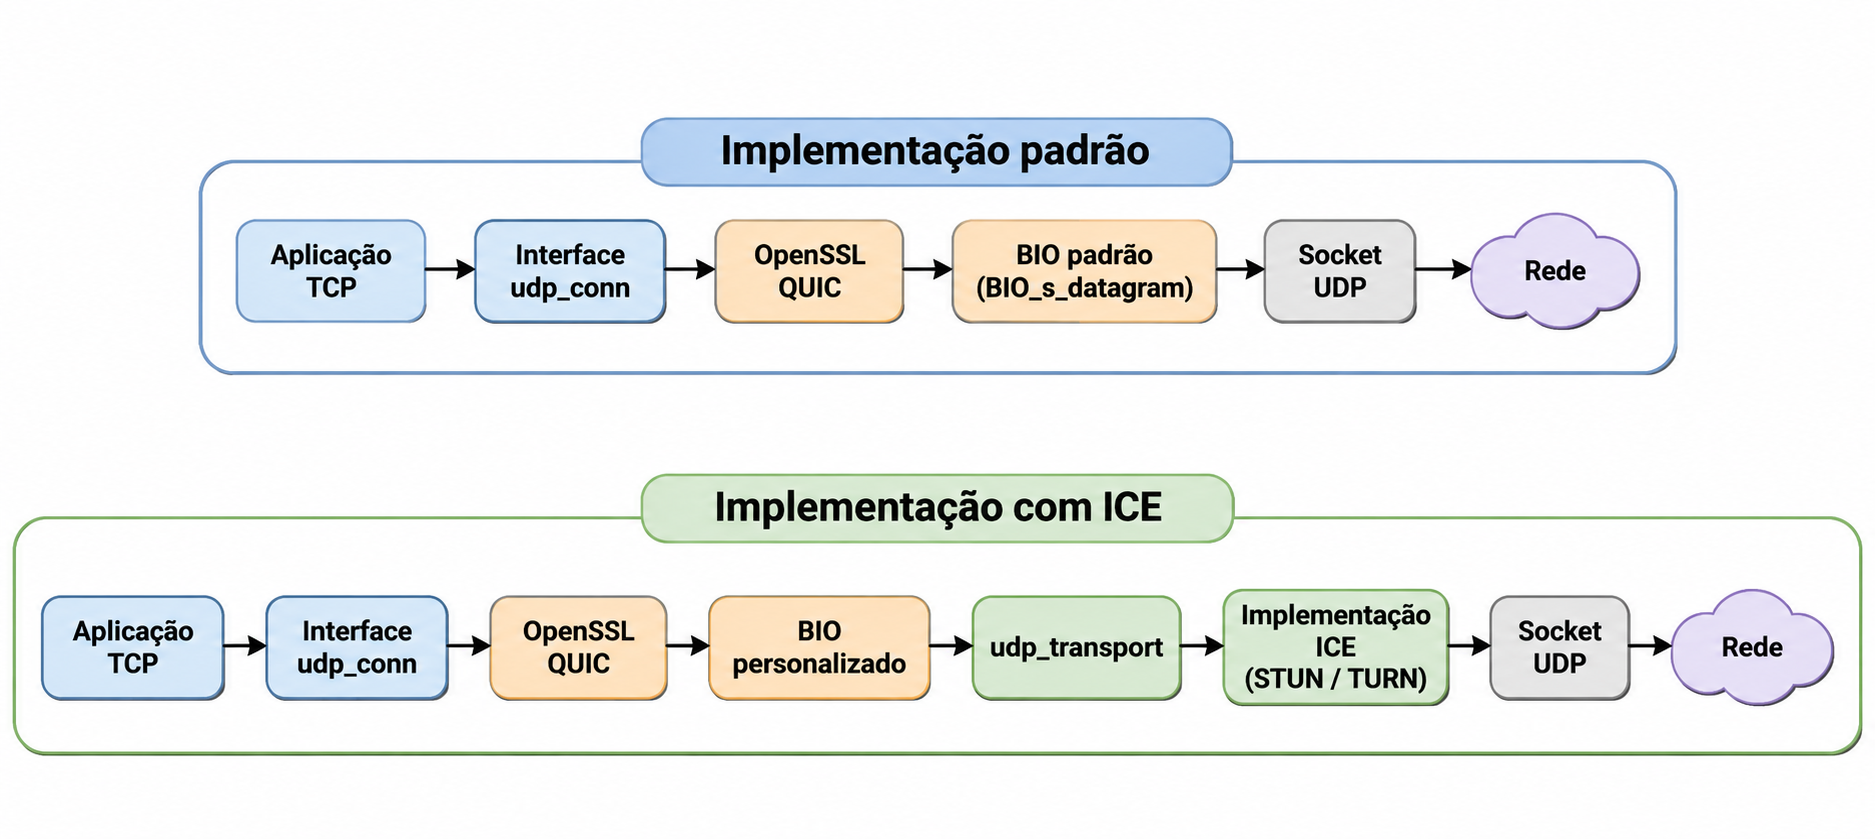
\includegraphics[width=0.9\textwidth]{fig/implementation/libnice/openssl_quic_bio_update.png}
    \caption{Diagrama de funcionamento do BIO OpenSSL juntamente com a interface \texttt{udp\_transport}.}
    \label{fig:openssl_quic_bio_update}
\end{figure}

O contrato necessário para a criação de um novo BIO, como no caso da implementação utilizada neste trabalho, é descrito por \citep{openssl_bio_meth} e exige a implementação dos seguintes métodos:

\begin{itemize}
    \item \textbf{create}: inicializar o estado específico de uma nova instância do BIO, cuja estrutura já foi alocada pela OpenSSL;
    \item \textbf{destroy}: liberar os recursos específicos da instância. A estrutura BIO em si é liberada pela OpenSSL;
    \item \textbf{ctrl}: atender comandos e consultas de controle, como \textit{flush}, configuração e obtenção de informações sobre o BIO;
    \item \textbf{sendmmsg}: enviar os datagramas fornecidos e informar quantas mensagens foram processadas;
    \item \textbf{recvmmsg}: receber datagramas nos \textit{buffers} fornecidos, preencher os tamanhos e endereços solicitados e informar quantas mensagens foram processadas.
\end{itemize}

\subsection{Funcionamento da integração da libnice}

Na arquitetura proposta, a integração da \texttt{libnice} é executada em cada \textit{gateway} e gerencia a conectividade com o \textit{gateway} remoto. Os candidatos ICE representam os caminhos disponíveis para a comunicação entre esses \textit{hosts}. Os dispositivos IoT associados ao cenário de aplicação não participam desse processo de negociação. 

Na integração da \texttt{libnice} com a interface \texttt{udp\_transport}, o usuário em nível de aplicação fica responsável apenas pela configuração desta interface, que se resume à configuração de IP/porta do servidor STUN, à configuração de IP/porta do servidor TURN e ao fornecimento de uma \textit{callback} responsável por realizar o processo de sinalização da forma que a aplicação encontrar mais adequada.

Durante as etapas de integração, grande parte das responsabilidades do protocolo ICE já são resolvidas diretamente na inicialização da interface. As configurações definidas pela aplicação são aplicadas à biblioteca, configurando cada um dos servidores. Após essa configuração, é realizada a coleta dos candidatos locais a partir dos servidores e da interface local; em seguida, é chamada a \textit{callback} definida pelo usuário para o tratamento do processo de sinalização, aguardando até que os candidatos remotos sejam recebidos. Ao recebê-los, são realizados os \textit{connectivity checks}, e, a partir da escolha dos endereços candidatos, o \textit{hole punching} é concluído, e o controle é liberado para a interface \texttt{udp\_conn}, restando como única responsabilidade pendente a gerência da conexão.

Como visto anteriormente, a \texttt{libnice} utiliza a \texttt{GLib}, uma biblioteca que fornece uma API baseada em eventos. Na implementação original da \texttt{udp\_conn}, era utilizada a chamada \texttt{select} para a gerência de múltiplas \textit{sockets}. Com a adesão da interface \texttt{udp\_transport}, essa chamada passou a ficar abstraída pela própria interface, já que ela é a responsável por gerenciar a \textit{socket} UDP. Com isso, a implementação ICE abandona o uso da chamada \texttt{select} em favor de uma variação da chamada \texttt{poll} da POSIX, também utilizada para gerenciar eventos. Dado o uso da \texttt{GLib}, a chamada utilizada é a \texttt{g\_poll}, responsável por gerenciar eventos da \texttt{GLib} e que, na prática, também utiliza \texttt{poll} internamente, ou até mesmo a própria chamada \textit{select}. Portanto, o \textit{loop} de eventos descrito anteriormente na Seção~\ref{sec:api_and_event_loop} passa a ser gerenciado internamente pela implementação de \texttt{udp\_transport}, e a gerência da conexão ICE é tratada dentro desse \textit{event loop}. Desta forma, o novo fluxo de conexão após a atualização com a biblioteca ICE se resume como visto pela Figura \ref{fig:udp_transport_connection_flow}.

\begin{figure}[ht]
    \centering
    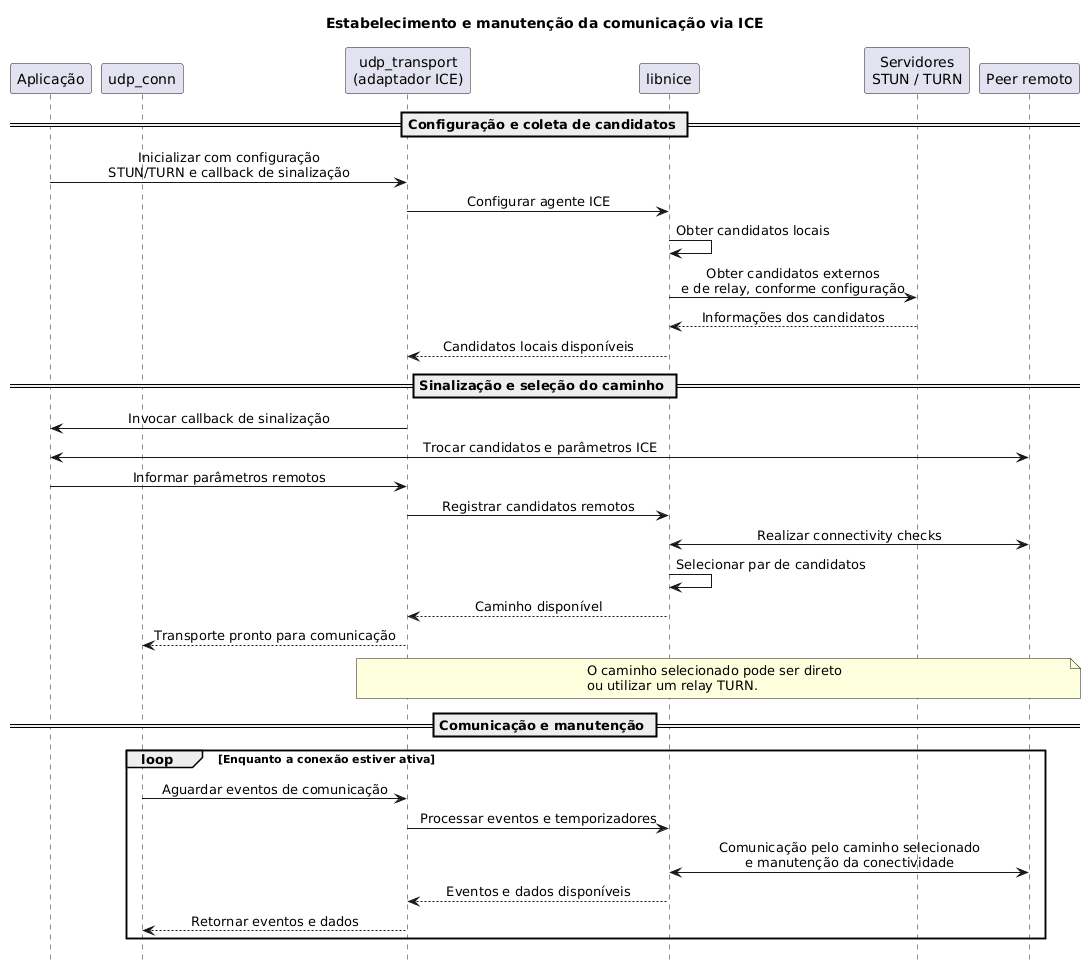
\includegraphics[width=0.8\textwidth]{fig/implementation/libnice/udp_transport_connection_flow.png}
    \caption{Diagrama de sequência do novo fluxo de conexão utilizando a biblioteca \texttt{libnice}.}
    \label{fig:udp_transport_connection_flow}
\end{figure}

\begin{comment}
    
\section{Implementação simplificada do QUIC}
\cgk{A ser feito (Implementação manual)}

\subsection{Implementação Simplificada da Conexão e Comunicação do QUIC}

\subsection{Implementação Simplificada de Connection Migration}

\subsection{Realização de Connection Migration Hole Punching}

\end{comment}

\begin{comment}
1. Transporte comum: UDP direto e ICE usam a mesma HAL. A libnice controla seus sockets, e o chamador processa eventos e timers pelo wait(), sem thread dedicada do adaptador.
2. ICE/STUN/TURN: coleta de candidatos, troca por callback de signaling, seleção do par e opção force_relay. Há testes de NAT, remapeamento de porta e TURN obrigatório.
3. CHOWNAT sobre ICE: mantém o handshake 01 → 03 → 03. A função chownat_recv_control() controla o prazo das esperas, evitando que timers ICE consumam tentativas antecipadamente.
4. QUIC sobre ICE: OpenSSL recebe datagramas por um BIO próprio ligado à HAL. Cliente e servidor usam estabelecimento e shutdown não bloqueantes com prazo. Foram separados dois streams bidirecionais, um para dados e outro para controle/keep-alive, evitando inserir bytes de controle no túnel TCP.
5. Fechamento e patch da libnice: o adaptador continua processando respostas durante o fechamento. Além disso, o build compila libnice 0.1.21 com um patch que repete a remoção TURN quando recebe 438 Stale nonce. A dependência corrigida fica estática em _deps, sem substituir a biblioteca do sistema.
\end{comment}
\chapter{Resultados}
\label{chap:results}

Este capítulo apresenta a avaliação da infraestrutura de comunicação desenvolvida, com foco no estabelecimento de conectividade e na transferência de dados entre aplicações TCP associadas a \textit{gateways} situados em redes distintas. A avaliação busca verificar o funcionamento da integração entre QUIC e ICE, considerando os caminhos de comunicação selecionados, a preservação dos dados transportados e o comportamento da solução durante a manutenção e o encerramento das conexões, como proposto pelos cenários de teste do Capítulo~\ref{chap:implementation}.

Inicialmente, são descritos o ambiente experimental, os cenários de teste e os critérios utilizados para analisar os resultados. Em seguida, são apresentados os testes de funcionamento e as medições de desempenho, relacionando as observações aos objetivos do trabalho. A discussão limita-se às configurações e às condições efetivamente avaliadas, sem pressupor a validação de um sistema IoT completo.

Além disso, são propostas na Seção~\ref{sec:another_connection_approaches} outras possíveis abordagens a serem comparadas apenas em nível lógico, o que implica que essa comparação não foi feita a partir de cenários de teste, mas apenas a partir dos conhecimentos previamente descritos nos Capítulos~\ref{chap:background} e~\ref{chap:quic}.

\section{Objetivo e metodologia da avaliação}

A avaliação tem como objetivo verificar se a infraestrutura desenvolvida permite estabelecer comunicação e transportar corretamente dados entre aplicações TCP associadas a \textit{gateways} situados em redes distintas. Os testes abrangem a integração entre QUIC e ICE, considerando o estabelecimento da conexão, a transferência bidirecional de dados, a manutenção da sessão e o encerramento dos recursos utilizados.

A metodologia compreende testes funcionais e medições de desempenho. Os testes funcionais verificam o comportamento da solução em cenários com comunicação direta e com retransmissão por TURN. A correção da transferência é verificada pela comparação entre os dados enviados e recebidos pelas aplicações. Nos testes de manutenção, são intercalados períodos de transferência e de inatividade para observar a continuidade da comunicação na mesma sessão.

Uma execução funcional é considerada bem-sucedida quando o caminho de comunicação esperado é selecionado, a conexão é estabelecida dentro do prazo definido, os dados são transferidos sem divergências e o encerramento ocorre sem erros. 

As medições de desempenho consideram o tempo de estabelecimento da comunicação, o tempo de resposta das aplicações e a vazão útil. Cada intervalo de medição é delimitado por eventos explícitos da execução, distinguindo o estabelecimento completo da infraestrutura do \textit{handshake} QUIC isolado. Os parâmetros de carga, a quantidade de repetições e os procedimentos de coleta são definidos para cada experimento e mantidos equivalentes nos cenários comparados.

Os testes utilizam dados sintéticos para avaliar o transporte entre os \textit{gateways}. A avaliação não inclui aquisição de dados por sensores físicos ou validação de requisitos de uma aplicação IoT específica. As conclusões são restritas aos ambientes, às configurações e às cargas efetivamente utilizados.

\section{Ambiente experimental e cenários com PatchBay}
\label{sec:experimental_patchbay}

Os experimentos utilizam as topologias descritas nas Seções~\ref{sec:basic_topology_network_namespaces}  e~\ref{sec:ice_topology_network_namespaces}, executadas com o PatchBay sobre \textit{Linux Network Namespaces}. Esta seção registra a configuração do ambiente e as diferenças entre os cenários de teste. A organização das interfaces de transporte e dos protocolos é apresentada no Capítulo~\ref{chap:implementation}.

\subsection{Plataforma e serviços auxiliares}

Os testes foram executados em ambientes com Ubuntu 24.04 LTS e Rocky Linux 8.10. A Tabela~\ref{tab:experimental_software} apresenta as versões das dependências utilizadas.

\begin{table}[htbp]
    \centering
    \label{tab:experimental_software}
    \begin{tabular}{@{}p{0.22\textwidth}p{0.14\textwidth}p{\dimexpr0.64\textwidth-4\tabcolsep\relax}@{}}
        \toprule
        \textbf{Componente} & \textbf{Versão} & \textbf{Função} \\
        \midrule
        OpenSSL & 4.1.0 &
        Implementação QUIC e proteção criptográfica. \\
        \texttt{libnice} & 0.1.21 &
        Coleta de candidatos, negociação ICE e transporte
        direto ou via TURN. \\
        \texttt{coturn} & 4.6.3 &
        Fornecimento dos serviços STUN e TURN. \\
        PatchBay & 0.7.0 &
        Criação e configuração da rede de testes. \\
        \bottomrule
    \end{tabular}
    \caption{Software utilizado no ambiente experimental.}
\end{table}

Os serviços auxiliares executam no nó ISP, conforme a topologia ICE apresentada na Seção~\ref{sec:ice_topology}. Sua configuração é resumida na Tabela~\ref{tab:experimental_services}.

\begin{table}[htbp]
    \centering
    \label{tab:experimental_services}
    \begin{tabular}{@{}p{0.28\textwidth}p{\dimexpr0.72\textwidth-2\tabcolsep\relax}@{}}
        \toprule
        \textbf{Elemento} & \textbf{Configuração} \\
        \midrule
        STUN/TURN &
        Comunicação por UDP, na porta 3478.
        O adaptador utiliza
        \texttt{NICE\_RELAY\_TYPE\_TURN\_UDP};
        TCP, TLS e DTLS estão desabilitados no servidor
        do laboratório. \\
        Autenticação TURN &
        Credenciais de longo prazo, com usuário e senha
        estáticos de laboratório e \textit{realm}
        \texttt{ice-test}. \\
        Sinalização &
        Servidor TCP na porta 5555, utilizado para trocar
        candidatos e credenciais ICE
        (\texttt{ice-ufrag} e \texttt{ice-pwd}). \\
        Proteção QUIC &
        TLS 1.3, com certificado autoassinado e chave
        privada no servidor. A correspondência entre
        certificado e chave é verificada na configuração. \\
        Verificação de identidade &
        O cliente utiliza \texttt{SSL\_VERIFY\_NONE},
        sem validar o certificado do servidor.
        Não há autenticação mútua por certificados. \\
        \bottomrule
    \end{tabular}
    \caption{Configuração dos serviços e da proteção QUIC.}
\end{table}

A configuração de certificados é restrita ao ambiente experimental. Os testes exercitam o transporte protegido pelo QUIC, mas não demonstram a validação da identidade do servidor remoto.

\subsection{Topologia e cenários de comunicação}
\label{sec:experimental_scenarios}

A rede contém dois \textit{peers}, cada um atrás de um roteador NAT, conectados por um roteador ISP. Os \textit{peers} representam os \textit{gateways} da arquitetura e executam tanto a implementação quanto as aplicações TCP locais utilizadas nos testes de tunelamento.

Conforme as Figuras~\ref{fig:basic_topology} e~\ref{fig:ice_topology}, a estrutura da rede é mantida entre os cenários. As diferenças estão nas regras de NAT, nos serviços auxiliares habilitados e na escolha do transporte. As LANs são isoladas, embora utilizem o mesmo prefixo \texttt{192.168.80.0/24}; a rede entre o ISP e os roteadores utiliza \texttt{10.0.0.0/24}.

Os roteadores partem do perfil \texttt{Moderate} do PatchBay. Nos cenários sem ICE, regras adicionais preservam a porta de origem, permitindo o conhecimento prévio dos endpoints públicos, como descrito na Seção~\ref{sec:basic_topology_hole_punching}. Nos cenários com ICE, a descoberta e a seleção dos endpoints são realizadas pela \texttt{libnice}, conforme a Seção~\ref{sec:ice_library}.

A Tabela~\ref{tab:experimental_scenarios} organiza os cenários por configuração de conectividade. Uma mesma configuração pode ser exercitada por mais de um teste.

\begin{table}[htbp]
    \centering
    \small
    \label{tab:experimental_scenarios}
    \begin{tabular}{@{}p{0.20\textwidth}p{0.38\textwidth}p{\dimexpr0.42\textwidth-4\tabcolsep\relax}@{}}
        \toprule
        \textbf{Cenário} &
        \textbf{Configuração} &
        \textbf{Objetivo} \\
        \midrule
        Comunicação sem ICE &
        UDP direto, endpoints previamente conhecidos
        e mapeamento de portas espelhado. &
        Exercitar Chownat e QUIC, com e sem tunelamento
        TCP, na topologia básica. \\
        Transporte ICE direto &
        STUN e sinalização habilitados, sem
        obrigatoriedade de relay. &
        Verificar a seleção de um caminho direto
        e a troca de datagramas pela interface
        \texttt{udp\_transport}. \\
        ICE com remapeamento de porta &
        Regras adicionais fazem a porta pública
        diferir da porta local. &
        Verificar a comunicação sem depender
        da preservação da porta de origem. \\
        Transporte ICE via TURN &
        TURN configurado e opção
        \texttt{force\_relay} habilitada. &
        Verificar o transporte de datagramas por
        um par de candidatos relay. \\
        Chownat sobre ICE &
        Tunelamento TCP com seleção ICE direta
        ou TURN obrigatório. &
        Verificar a integração do Chownat com
        ambos os caminhos de transporte. \\
        QUIC sobre ICE &
        Tunelamento TCP com seleção ICE direta
        ou TURN obrigatório. &
        Verificar a integração QUIC/ICE por meio
        do BIO descrito na
        Figura~\ref{fig:openssl_quic_bio_update}. \\
        \bottomrule
    \end{tabular}
    \caption{Cenários de comunicação avaliados com PatchBay.}
\end{table}

Nos cenários diretos, os servidores auxiliam o estabelecimento da comunicação, enquanto os dados da aplicação trafegam entre os \textit{peers}. Nos cenários TURN, os dados passam pelo servidor relay, conforme a Figura~\ref{fig:turn_quic_tcp_tunneling}.

O uso de \texttt{force\_relay} torna obrigatório o caminho TURN mesmo quando um caminho direto poderia existir. Portanto, esses testes verificam a operação via relay, sem representar, por si só, uma falha de conectividade direta causada por um NAT mais restritivo. 

Há também um teste prolongado de QUIC sobre TURN, destinado a verificar a manutenção da sessão e a renovação dos recursos TURN. A duração e a carga aplicada são apresentadas na seção de cargas de trabalho e coleta das medições.

\subsection{Parâmetros de execução}

A Tabela~\ref{tab:experimental_parameters} apresenta os prazos e limites definidos pela implementação e pelas configurações dos testes. Esses valores se aplicam às etapas indicadas e não constituem um prazo global de execução. Importante destacar que a maior parte destes parÂmetros são configuráveis pela camada de aplicação.

\begin{table}[htbp]
    \centering
    \label{tab:experimental_parameters}
    \begin{tabular}{@{}p{0.49\textwidth}p{0.10\textwidth}p{\dimexpr0.41\textwidth-4\tabcolsep\relax}@{}}
        \toprule
        \textbf{Parâmetro} &
        \textbf{Valor} &
        \textbf{Aplicação} \\
        \midrule
        Espera pela prontidão do ICE &
        5~s & Chownat/ICE e QUIC/ICE \\
        Leitura/escrita da sinalização &
        3~s & Chownat/ICE e QUIC/ICE \\
        Estabelecimento QUIC e abertura dos streams &
        5~s & Testes QUIC \\
        Espera por resposta de controle Chownat &
        1~s & Conexão e encerramento \\
        Limite de tentativas Chownat &
        5--20 & Com e sem ICE \\
        Inatividade para acionar \textit{keep-alive}
        da sessão &
        5~s & Camada \texttt{udp\_conn} \\
        Buffer de leitura e encaminhamento &
        1024~B & Túnel TCP na camada \texttt{udp\_conn} \\
        Limite de payload por datagrama UDP &
        1200~B & BIO utilizado pelo QUIC \\
        \bottomrule
    \end{tabular}
    \caption{Parâmetros de execução dos testes de comunicação.} 
\end{table}

O intervalo de \textit{keep-alive} indicado corresponde à camada de sessão descrita na
Seção~\ref{sec:api_and_event_loop}; os temporizadores internos do ICE e do QUIC são gerenciados pelas respectivas bibliotecas. O executor não configura explicitamente atraso, perda de pacotes ou limitação de banda nos enlaces.

Como os \textit{namespaces} compartilham o mesmo \textit{kernel} e os recursos da máquina hospedeira, os resultados caracterizam esse ambiente local de execução, conforme discutido na Seção~\ref{sec:linux_network_namespaces}.









\section{Resultados dos testes funcionais}
\label{sec:functional_results}

A avaliação funcional investigou três propriedades da integração: a descoberta de um caminho entre gateways sem conhecimento prévio das portas públicas, a preservação dos dados das aplicações TCP e a manutenção e liberação dos recursos utilizados pelo transporte. Para relacionar essas propriedades à implementação do Capítulo~\ref{chap:implementation}, foram examinados os pacotes capturados em diferentes interfaces, os pares selecionados pela \texttt{libnice} e as verificações de conteúdo realizadas pelos testes.

A Tabela~\ref{tab:functional_cases} identifica os casos avaliados nesta seção. Os códigos C1 a C13 são utilizados ao longo da análise para relacionar cada resultado à configuração e à verificação correspondente. C1 a C12 são casos da suíte regular executada em poucos segundos; C13 corresponde ao teste prolongado com cerca de aproximadamente 10 minutos de simulação.

\begin{table}[htbp]
    \centering
    \small
    \label{tab:functional_cases}
    \begin{tabular}{@{}p{0.07\textwidth}p{0.40\textwidth}p{\dimexpr0.53\textwidth-4\tabcolsep\relax}@{}}
        \toprule
        \textbf{Caso} & \textbf{Configuração} & \textbf{Verificação} \\
        \midrule
        C1 & Chownat sem ICE, sem túnel TCP & Três rodadas de requisição/resposta e encerramento. \\
        C2 & Chownat sem ICE, encerramento dedicado & Troca de 20/21 mensagens e liberação da sessão. \\
        C3 & Chownat sem ICE, com túnel TCP & Transferência de 16384 bytes por sentido. \\
        C4 & QUIC sem ICE, sem túnel TCP & Três rodadas de requisição/resposta e encerramento. \\
        C5 & QUIC sem ICE, com túnel TCP & Transferência de 16384 bytes por sentido. \\
        C6 & Transporte ICE direto & Troca bidirecional de datagramas pelo par selecionado. \\
        C7 & Transporte ICE com remapeamento & Descoberta de portas públicas diferentes das locais e troca de datagramas. \\
        C8 & Transporte ICE via TURN obrigatório & Troca de datagramas por relay e remoção das allocations. \\
        C9 & Chownat/ICE direto, com túnel TCP & Transferência de 16384 bytes por sentido. \\
        C10 & Chownat/ICE via TURN, com túnel TCP & Transferência de 16384 bytes por sentido e remoção das allocations. \\
        C11 & QUIC/ICE direto, com túnel TCP & Transferência de 16384 bytes por sentido. \\
        C12 & QUIC/ICE via TURN, com túnel TCP & Transferência de 16384 bytes por sentido e remoção das allocations. \\
        C13 & QUIC/ICE via TURN, sessão prolongada & 67 blocos de 16384 bytes por sentido, renovação e remoção dos recursos TURN. \\
        \bottomrule
    \end{tabular}
    \caption{Casos avaliados nos testes funcionais.}
\end{table}

Os resultados a seguir detalham as evidências desses casos. As figuras reservadas nesta seção correspondem a recortes das capturas e devem ser inseridas conforme as indicações nos comentários.

\subsection{Estabelecimento da comunicação e caminhos selecionados}
\label{sec:functional_establishment}

A primeira diferença observável entre os transportes direto e ICE é a obtenção do endpoint remoto. Nos casos sem ICE (C1--C5), Chownat e QUIC utilizam os endereços previamente configurados e o mapeamento de portas espelhado descrito na Seção~\ref{sec:basic_topology_hole_punching}. A comunicação nesses casos estabelece a referência funcional para a comparação com o adaptador ICE. A descoberta e a negociação acrescentadas por esse adaptador são examinadas pelo caso C7, com remapeamento de porta.

No caso C7, a captura da interface LAN do gateway A registra um Binding Request originado em \texttt{192.168.80.20:54960}. A mesma transação aparece na WAN do roteador A com origem \texttt{10.0.0.2:38576}. A resposta STUN contém esse último endpoint no atributo \texttt{XOR-MAPPED-ADDRESS} como é possível ver na Figura \ref{fig:result_stun_remap}. A associação entre as duas capturas é feita pelo identificador da transação STUN, preservado durante a tradução. Portanto, a diferença entre as portas não é apenas uma configuração declarada: ela aparece nos pacotes efetivamente enviados e na resposta utilizada para a descoberta.

\begin{figure}[htbp]
    \centering
    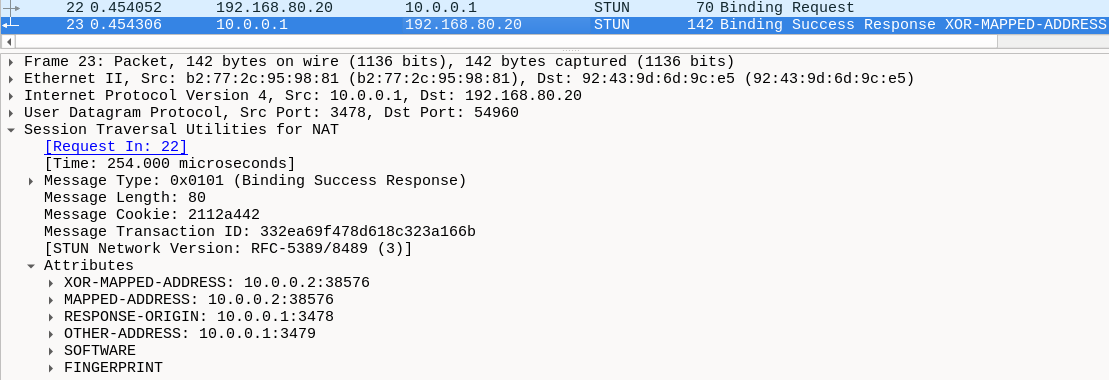
\includegraphics[width=1.0\textwidth]{fig/results/tests/stun_response_diff_mapping.png}
    \caption{Descoberta do endpoint público do gateway A no cenário
    com remapeamento.}
    \label{fig:result_stun_remap}
\end{figure}

Após a troca de candidatos, a WAN do roteador A registra um Binding Request destinado a \texttt{10.0.0.3:64027}, com \texttt{USERNAME}, \texttt{MESSAGE-INTEGRITY} e \texttt{USE-CANDIDATE}, seguido de uma resposta de sucesso. O destino é o endpoint público do gateway B, cuja porta local 47643 foi traduzida para 64027. A seleção registrada pela \texttt{libnice} corresponde ao par
\texttt{10.0.0.2:38576} e \texttt{10.0.0.3:64027}. Essa sequência vincula a descoberta, a nomeação do par e a comunicação posterior a portas públicas diferentes das portas locais. Assim, nesse cenário, o transporte ICE remove a dependência do ``mapeamento espelhado'' presente na referência sem ICE.

No caso C11 (QUIC/ICE direto), a captura permite acompanhar também a passagem da negociação ICE para o estabelecimento QUIC. Ao analisar a Figura \ref{fig:result_ice_quic_direct}, os quadros
26 e 27 contêm a nomeação e a resposta STUN, e descrevem as próprias etapas de UDP \textit{hole punching} a partir dos \textit{connectivity checks}. Posteriormente, o quadro 59 apresenta um datagrama UDP de 1200 bytes iniciado por um pacote QUIC Initial. A sequência inclui Retry e pacotes Handshake entre \texttt{10.0.0.2:49381} e \texttt{10.0.0.3:38368}. Esses são os \textit{endpoints} do par reflexivo selecionado nos \textit{logs}. Entre os \textit{checks} e o Initial aparecem os pequenos datagramas de controle do procedimento de descoberta mantido pelo \textit{backend} QUIC. A captura, portanto, permite distinguir a preparação do caminho do \textit{handshake} QUIC descrito na implementação.

% FIGURA 2: network_quic_ice_tcp/pcap/router-a/wan.pcap.
% Filtro: (frame.number >= 25 && frame.number <= 32) ||
%         (frame.number >= 59 && frame.number <= 73)
% Dois painéis: checks STUN (selecionar 26) e handshake (selecionar 59).
% Mostrar No., Time, Source, Destination, Protocol, Info e portas UDP.
% Sem chaves da sessão, não usar a imagem para afirmar validação de
% certificado nem para mostrar o conteúdo cifrado dos pacotes Handshake.
\begin{figure}[htbp]
    \centering
    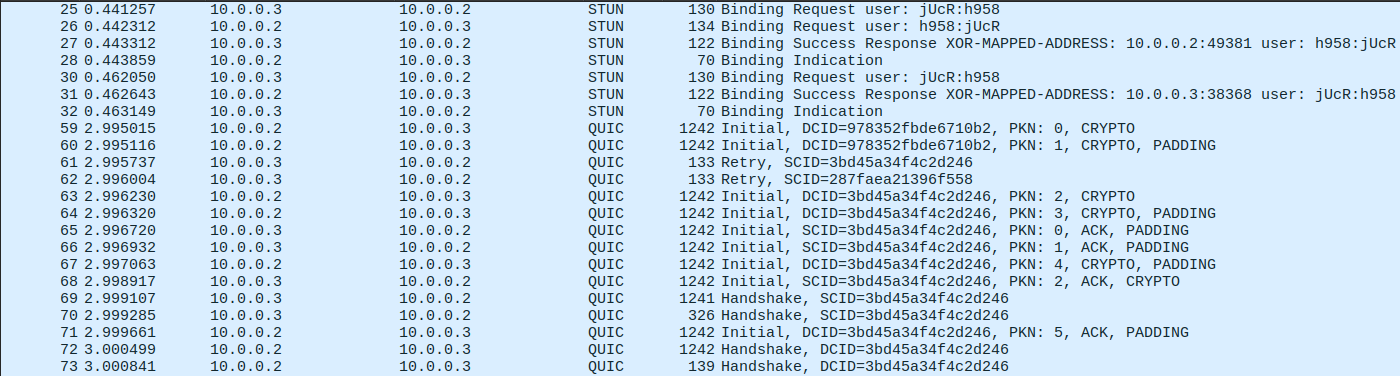
\includegraphics[width=1.0\textwidth]{fig/results/tests/cc_and_quic_handshake.png}
    \caption{Estabelecimento QUIC sobre o caminho ICE direto.}
    \label{fig:result_ice_quic_direct}
\end{figure}

A Tabela~\ref{tab:functional_paths} sintetiza as seleções da suíte regular (C1--C12). Nos quatro casos ICE diretos (C6, C7, C9 e C11), os dois candidatos foram identificados como reflexivos de servidor. Nos três casos com TURN obrigatório (C8, C10 e C12), ambos os candidatos eram relay.

\begin{table}[htbp]
    \centering
    \small
    \caption{Caminhos observados nos testes de estabelecimento.}
    \label{tab:functional_paths}
    \begin{tabular}{@{}p{0.43\textwidth}p{\dimexpr0.57\textwidth-2\tabcolsep\relax}@{}}
        \toprule
        \textbf{Cenários} & \textbf{Caminho observado} \\
        \midrule
        C1--C5: Chownat e QUIC sem ICE & UDP direto, com endpoints configurados previamente. \\
        C6 e C7: transporte ICE direto e com remapeamento & Par reflexivo de servidor/reflexivo de servidor. \\
        C9 e C11: Chownat/ICE e QUIC/ICE diretos & Par reflexivo de servidor/reflexivo de servidor. \\
        C8, C10 e C12: transporte ICE, Chownat/ICE e QUIC/ICE via TURN & Par relay/relay, com allocations no servidor. \\
        \bottomrule
    \end{tabular}
\end{table}

O uso de TURN altera o caminho de dados, além da seleção informada pela biblioteca. No caso C12 (QUIC/ICE/TURN), a resposta \textit{Allocate} informa \texttt{10.0.0.1:49191} como endereço de \textit{relay} do \textit{gateway} A. O ChannelBind associa o canal \texttt{0x4000} ao \textit{relay} remoto \texttt{10.0.0.1:49172}; em seguida, a WAN registra mensagens ChannelData entre \texttt{10.0.0.2:47158} e o servidor \texttt{10.0.0.1:3478}. No quadro 64, como visto na Figura \ref{fig:result_turn_data_path}, uma dessas mensagens contém 1200 \textit{bytes} de dados encapsulados, além do cabeçalho ChannelData de quatro \textit{bytes}. A captura evidencia, assim, o encapsulamento acrescentado pelo adaptador ICE sem alterar a interface utilizada pelo \textit{backend} QUIC (Figura~\ref{fig:openssl_quic_bio_update}).

\begin{figure}[htbp]
    \centering
    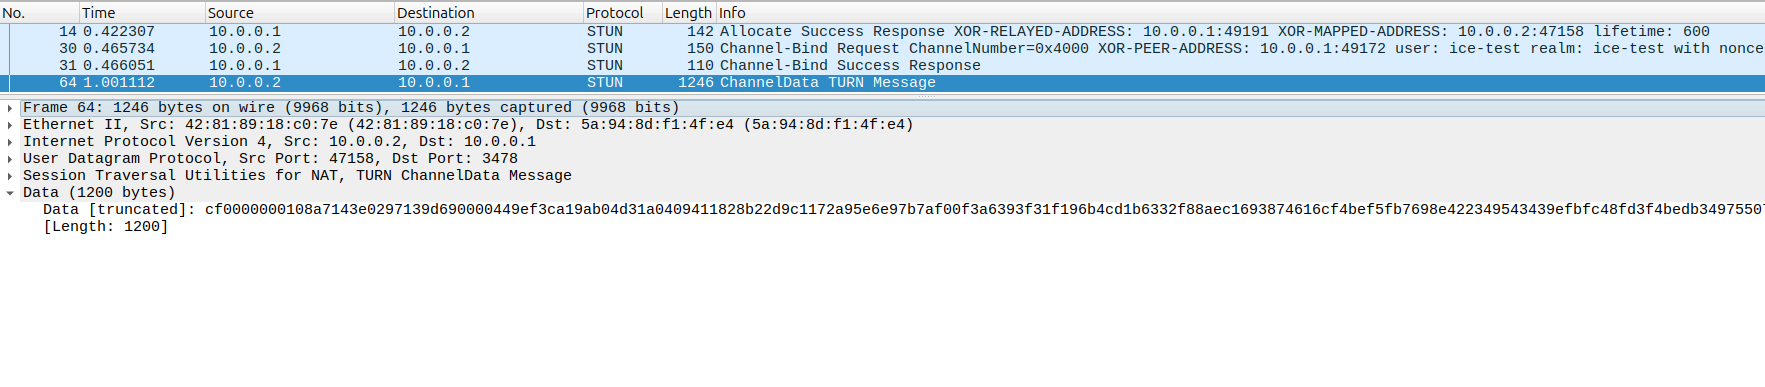
\includegraphics[width=1.0\textwidth]{fig/results/tests/turn_allocate_data_transfer.png}
    \caption{Caminho QUIC/ICE via TURN: \textit{allocation}, associação do canal
    ao relay remoto e transporte de dados por ChannelData.}
    \label{fig:result_turn_data_path}
\end{figure}

Os casos C8, C10, C12 e C13 utilizam \texttt{force\_relay} (opção que obriga a \texttt{libnice} a utilizar um servidor \textit{relay}). Demonstram o transporte pelo servidor quando esse caminho é imposto, mas não avaliam a transição automática de uma tentativa direta malsucedida para TURN.

\subsection{Transferência de dados e integração com aplicações TCP}
\label{sec:functional_data_transfer}

A verificação dos dados foi realizada nas interfaces entregues às aplicações, pois a conclusão do \textit{handshake} não demonstra que o túnel preserva o conteúdo transmitido. Nos seis casos curtos de túnel TCP (C3, C5 e C9--C12), o gerador enviou 16384 bytes e comparou a resposta do serviço \textit{echo} byte a byte.

O caso C11 (QUIC/ICE direto) ilustra a relação entre as duas conexões TCP locais e o transporte entre \textit{gateways}. No \textit{gateway} A, a aplicação se conecta à porta 44444, e o quadro 86 da captura de \textit{loopback} (Figura \ref{fig:result_tcp_application}(a)) contém os 16384 bytes entregues ao túnel. No \textit{gateway} B (Figura \ref{fig:result_tcp_application}(b)), a implementação abre outra conexão TCP com o serviço \textit{echo} na porta 1234. Nessa segunda conexão, o primeiro segmento de dados observado contém 1024 bytes, e os demais completam a mesma sequência de aplicação. As fronteiras dos segmentos são diferentes, enquanto o conteúdo entregue ao serviço é preservado.

\begin{figure}[htbp]
    \centering

    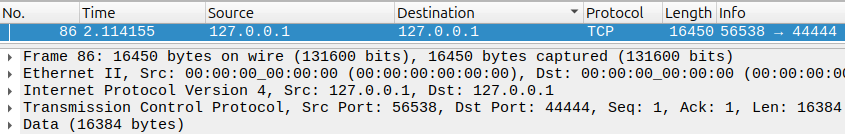
\includegraphics[width=0.90\linewidth]{fig/results/tests/tcp_local_payload.png}
    \\ Gateway A — envio dos dados TCP
    
    \par\medskip

    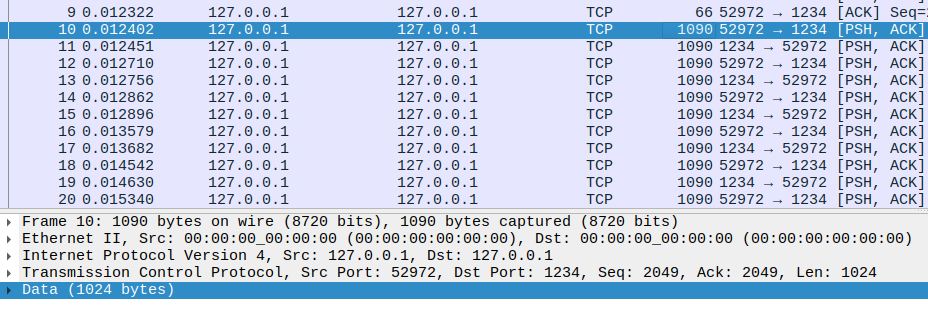
\includegraphics[width=0.90\linewidth]{fig/results/tests/tcp_remote_payload.png}
    \\ Gateway B — recepção dos dados TCP

    \caption{Integração com aplicações TCP no cenário QUIC/ICE direto.}
    \label{fig:result_tcp_application}
\end{figure}

Para conferir o conteúdo além do recorte visual, os dados foram reconstruídos a partir dos números de sequência TCP dessas duas capturas. Os quatro fluxos unidirecionais, correspondentes à ida e à volta em cada gateway, continham exatamente 16384 bytes, sem lacunas, e eram idênticos ao payload de referência. Isso relaciona os bytes enviados pela aplicação aos recebidos pelo serviço remoto e aos devolvidos na resposta. A evidência sustenta o tunelamento de dados descrito na Figura~\ref{fig:udp_conn_tcp_tunneling_diagram}: os segmentos TCP pertencem às conexões locais, e os dados atravessam a rede externa pelo transporte QUIC selecionado.

\begin{table}[htbp]
    \centering
    \small
    \caption{Resultados das verificações de conteúdo e entrega às aplicações.}
    \label{tab:functional_transfer}
    \begin{tabular}{@{}p{0.36\textwidth}p{\dimexpr0.64\textwidth-2\tabcolsep\relax}@{}}
        \toprule
        \textbf{Grupo de testes} & \textbf{Resultado observado} \\
        \midrule
        C1 e C4: Chownat e QUIC sem túnel & Três rodadas de requisição/resposta com conteúdo e sequência conferidos por protocolo. \\
        C6--C8: transporte ICE direto, remapeado e via TURN & Mensagens recebidas nos dois sentidos com conteúdo e tamanho esperados. \\
        C3, C9 e C10: Chownat com túnel TCP & Echo de 16384 bytes íntegro nas variantes sem ICE, ICE direto e ICE/TURN. \\
        C5, C11 e C12: QUIC com túnel TCP & Echo de 16384 bytes íntegro nas variantes sem ICE, ICE direto e ICE/TURN. \\
        \bottomrule
    \end{tabular}
\end{table}

No caso C2, dedicado ao encerramento Chownat, foram verificadas 20 mensagens recebidas no cliente e 21 no servidor, seguidas do fechamento e da liberação da sessão. Indicando o correto funcionamento configurado baseado no limite de tentativas do Chownat descrito na Tabela \ref{tab} que são utilizados tanto para tentativas de início de conexão tanto para o limíte de pacotes de \textit{keep-alive} enviados até considerar que uma conexão foi finalizada.

Nas quatro integrações de túnel com ICE (C9--C12), os contadores dos peers também registraram 16384 bytes enviados e recebidos por extremo e um único evento de conexão estabelecida. O resultado simultâneo nas variantes direta e TURN indica que a escolha do caminho ficou encapsulada no transporte, mantendo a entrega esperada pelas aplicações TCP locais. Essa conclusão se refere às cargas e às condições de rede exercitadas nesta coleta.

\subsection{Manutenção e encerramento das conexões}
\label{sec:functional_maintenance_shutdown}

Uma execução curta pode concluir a transferência antes de ser necessário renovar os recursos TURN. Por isso, o caso C13 manteve a sessão QUIC/ICE/TURN durante 67 transferências, com intervalos de 10~s entre os blocos a partir do segundo envio. Cada peer confirmou 1097728 bytes enviados e recebidos, e o teste completo, incluindo preparação e encerramento, terminou em 663,81~s. Sua duração permitiu observar renovações durante a mesma sessão.

A captura do gateway A mostra novos pedidos CreatePermission aproximadamente aos 241 e 481~s, ambos respondidos com sucesso. Aos 540~s, aparecem um Refresh e um ChannelBind, também seguidos de respostas de sucesso; a resposta ao Refresh informa \texttt{LIFETIME=600}. A Tabela~\ref{tab:functional_lifecycle} situa essas transações na captura, e a Figura~\ref{fig:result_turn_renewals} reserva os recortes correspondentes. Os registros do servidor confirmam as mesmas operações para a sessão do outro gateway.

\begin{table}[htbp]
    \centering
    \small
    \caption{Transações de manutenção e remoção na captura do gateway A
    durante o caso C13. Tempos relativos ao início dessa captura.}
    \label{tab:functional_lifecycle}
    \begin{tabular}{@{}p{0.15\textwidth}p{0.24\textwidth}p{\dimexpr0.61\textwidth-4\tabcolsep\relax}@{}}
        \toprule
        \textbf{Tempo (s)} & \textbf{Quadros} & \textbf{Transação e resposta} \\
        \midrule
        241,29 & 1312--1313 & CreatePermission e resposta de sucesso. \\
        481,73 & 2456--2457 & Nova renovação de permissão e resposta de sucesso. \\
        540,54 & 2757--2760 & Refresh com resposta LIFETIME 600 e renovação ChannelBind. \\
        662,14 & 3371--3374 & Remoção com LIFETIME zero, erro 438, novo pedido e sucesso. \\
        \bottomrule
    \end{tabular}
\end{table}

\begin{figure}[htbp]
    \centering
    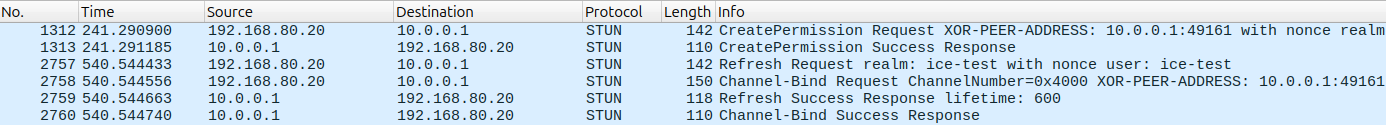
\includegraphics[width=1.0\linewidth]{fig/results/tests/renewals.png}
    \caption{Renovação dos recursos TURN durante a sessão QUIC/ICE.}
    \label{fig:result_turn_renewals}
\end{figure}

No encerramento do caso C13, o \textit{gateway} A solicita a remoção da allocation com \texttt{LIFETIME=0}, Como o \textit{nonce} utilizado já havia expirado, o servidor responde com erro 438 (\textit{Stale Nonce}) e fornece um novo \textit{nonce}. Em seguida, envia outro \textit{Refresh} com o \textit{nonce} fornecido nessa resposta e recebe sucesso com tempo de vida zero. Os dois pares de mensagens possuem identificadores de transação distintos: trata-se de um novo pedido autenticado, e não apenas da retransmissão do datagrama anterior.

\begin{figure}[htbp]
    \centering
    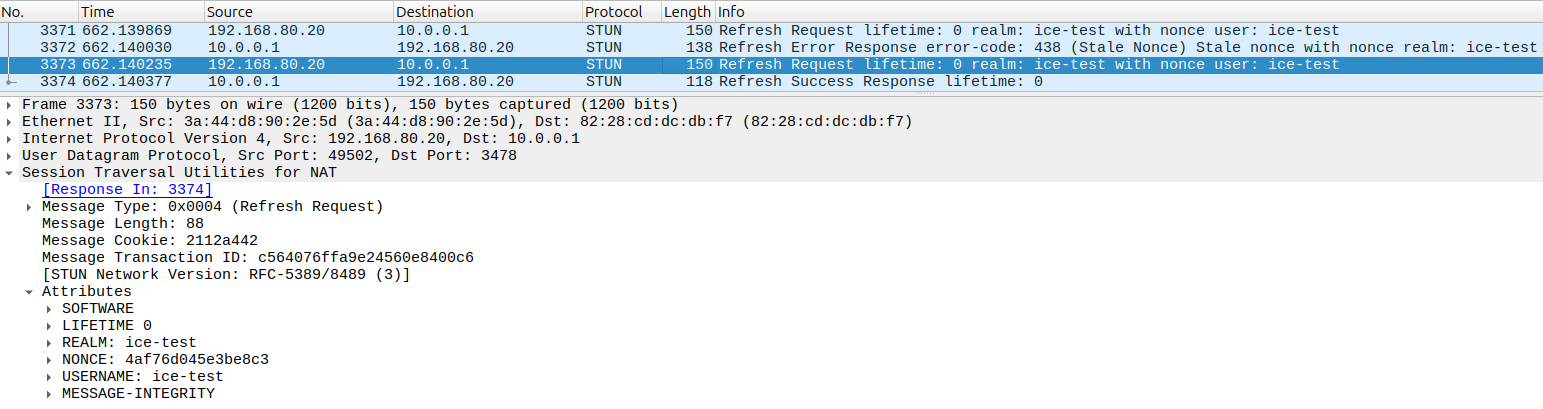
\includegraphics[width=1.0\linewidth]{fig/results/tests/turn_stale_nonce.png}
    \caption{Remoção da allocation TURN após expiração do nonce:
    tratamento do erro 438 e conclusão da nova transação de remoção.}
    \label{fig:result_turn_stale_nonce}
\end{figure}

Essa sequência permite verificar o efeito de uma correção aplicada à \texttt{libnice}. A correção faz a \texttt{libnice}, ao receber o erro 438 durante a remoção de uma allocation TURN, atualizar o nonce e repetir o pedido Refresh com \texttt{LIFETIME=0}. Antes, a biblioteca encerrava o procedimento localmente sem concluir a remoção no servidor. Com a correção, o recebimento do erro não encerrou o procedimento antes da remoção efetiva. O servidor registrou o erro 438 e a remoção com tempo de vida zero para os dois peers. Já o fechamento do túnel TCP é realizado localmente. O caso C13 demonstra a continuidade da transferência durante as renovações observadas e a conclusão do encerramento após erro 438.


\section{Avaliação em infraestrutura física controlada}
\subsection{Configuração dos equipamentos}
\subsection{Resultados e comparação com o ambiente PatchBay}

\cgk{adicionar esta implementação}



\section{Análise comparativa das abordagens de comunicação}
\label{sec:another_connection_approaches}

Para a análise lógica, foram propostos três cenários diferentes, contrapondo possíveis abordagens a serem utilizadas para a realização do mesmo tipo de comunicação: a abordagem P2P com ICE e QUIC desenvolvida neste trabalho; a abordagem mais comumente utilizada e aplicada na grande maioria dos dispositivos IoT, que segue um modelo de arquitetura do estilo cliente-servidor, a partir de um servidor especializado para a gerência das conexões; e uma abordagem P2P alternativa, utilizando comunicação TCP a partir de técnicas de TCP hole punching, como descritas na Seção~\ref{sec:tcp_hole_punching}.

\subsection{Comunicação P2P com ICE e QUIC}

Como base da análise lógica, pode-se utilizar a Figura~\ref{fig:non_centralized_quic_flow}, na qual é possível observar todo o processo lógico de conexão utilizando o ICE e, posteriormente, o protocolo QUIC para a conexão, e, após o estabelecimento desta, as trocas diretas entre cliente e servidor.

\begin{figure}[!ht]
    \centering
    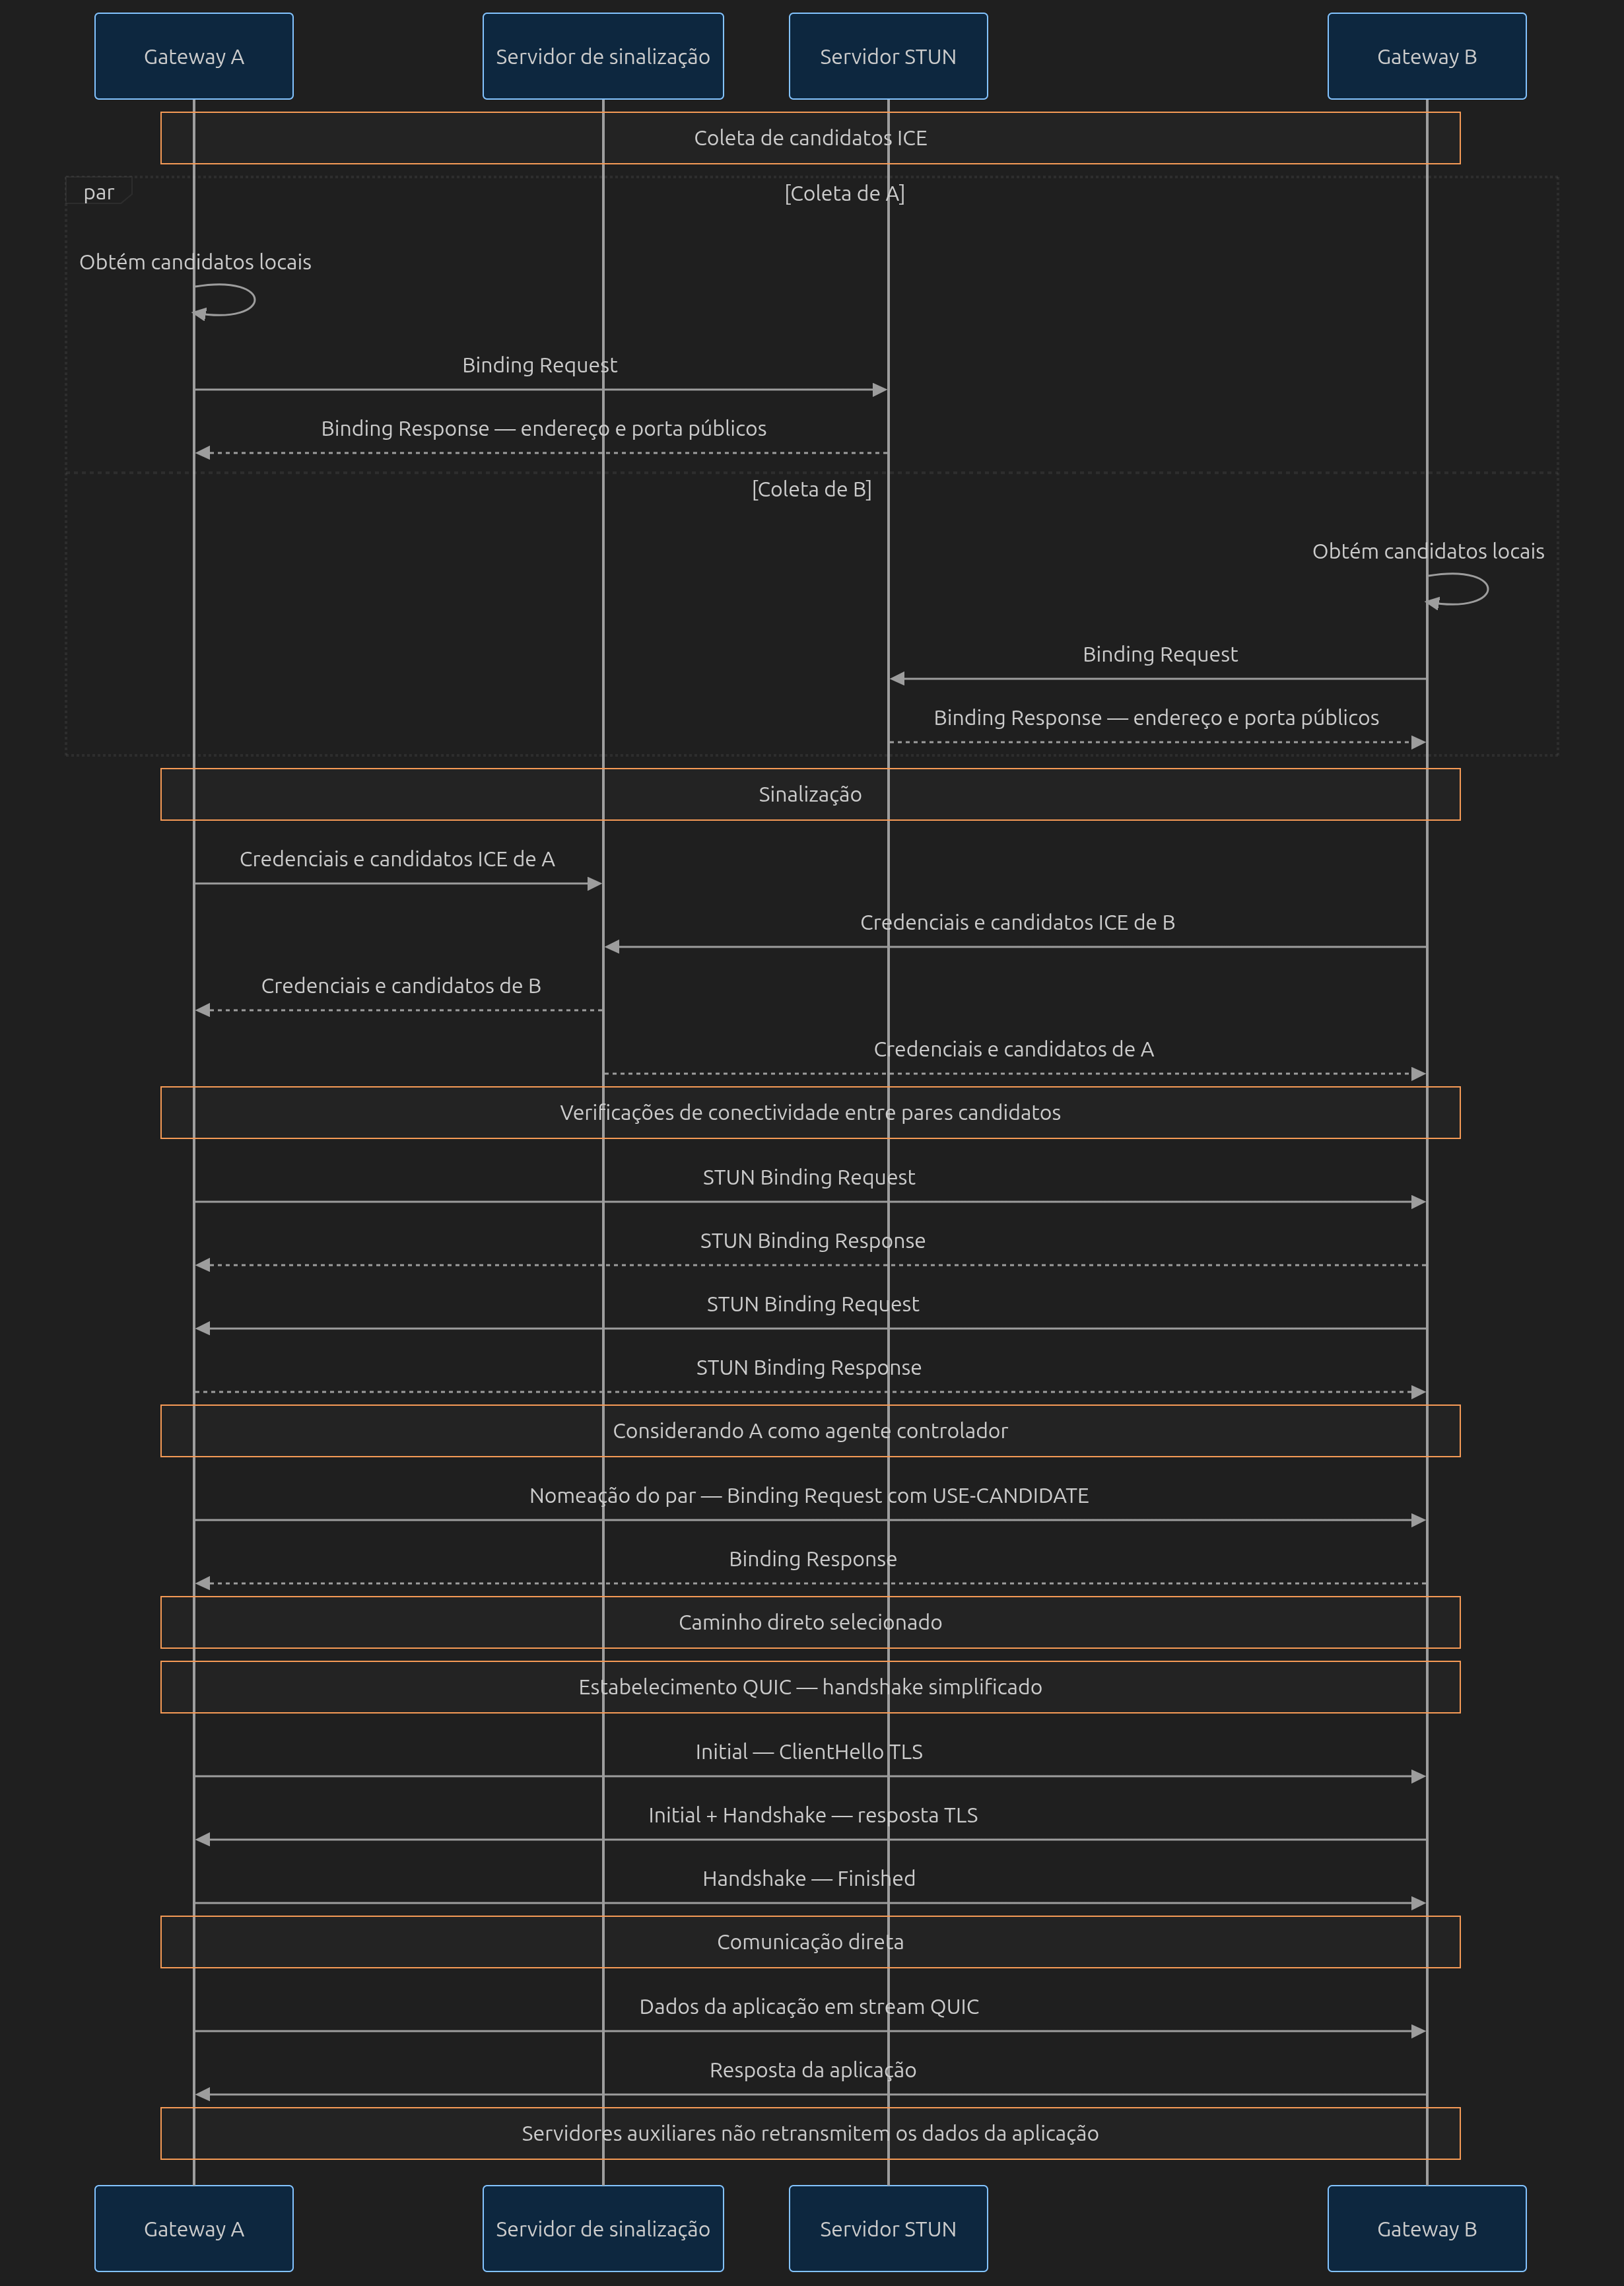
\includegraphics[width=0.8\textwidth]{fig/results/logic/flow_ice.png}
    \caption{Diagrama de tempo das etapas de comunicação utilizando o Protocolo ICE em união com o protocolo QUIC.}
    \label{fig:non_centralized_quic_flow}
\end{figure}

Importante lembrar que, ao utilizar um servidor TURN como \textit{fallback} -- isto é, caso a comunicação utilizando técnicas de \textit{hole punching} falhe --, ainda existiria um nível de indireção associado ao processo de estabelecimento, manutenção de conexão e troca de mensagens, acrescentando um custo adicional à comunicação.

\subsection{Comunicação com servidor intermediário especializado}

Ao se utilizar um servidor especializado, remove-se a obrigação do processamento em borda, o que aumenta a infraestrutura necessária. Para esta análise, o foco estará completamente nas etapas de conexão e no custo lógico de envio de mensagens entre os \textit{peers}; ainda assim, é importante manter em vista o custo infraestrutural envolvido, dado que a manutenção desse servidor também tem um custo. Nesta abordagem com um servidor intermediário, os dois \textit{peers} precisarão se conectar ao servidor, e, a partir disso, pacotes serão trocados entre eles. Suponha-se também um cenário ideal, no qual a comunicação entre \textit{peer} e servidor é feita por meio de um protocolo que já integra mecanismos de garantia de confidencialidade ao seu processo de conexão, como o QUIC -- caso fosse utilizado TCP/TLS, haveria ainda um custo adicional associado ao \textit{3-way handshake} do TLS.

A Figura~\ref{fig:centralized_server_quic_flow} descreve cada uma das etapas associadas a essa comunicação, sendo perceptível a diferença em relação ao fluxo descrito na Figura~\ref{fig:non_centralized_quic_flow}, principalmente quanto ao custo do uso do ICE nas etapas de estabelecimento da conexão da abordagem P2P. Em contrapartida, após o estabelecimento da conexão P2P, as mensagens são enviadas diretamente entre os pares, enquanto na abordagem com servidor especializado existe sempre um nível de indireção associado à retransmissão pelo servidor.

\begin{figure}[!ht]
    \centering
    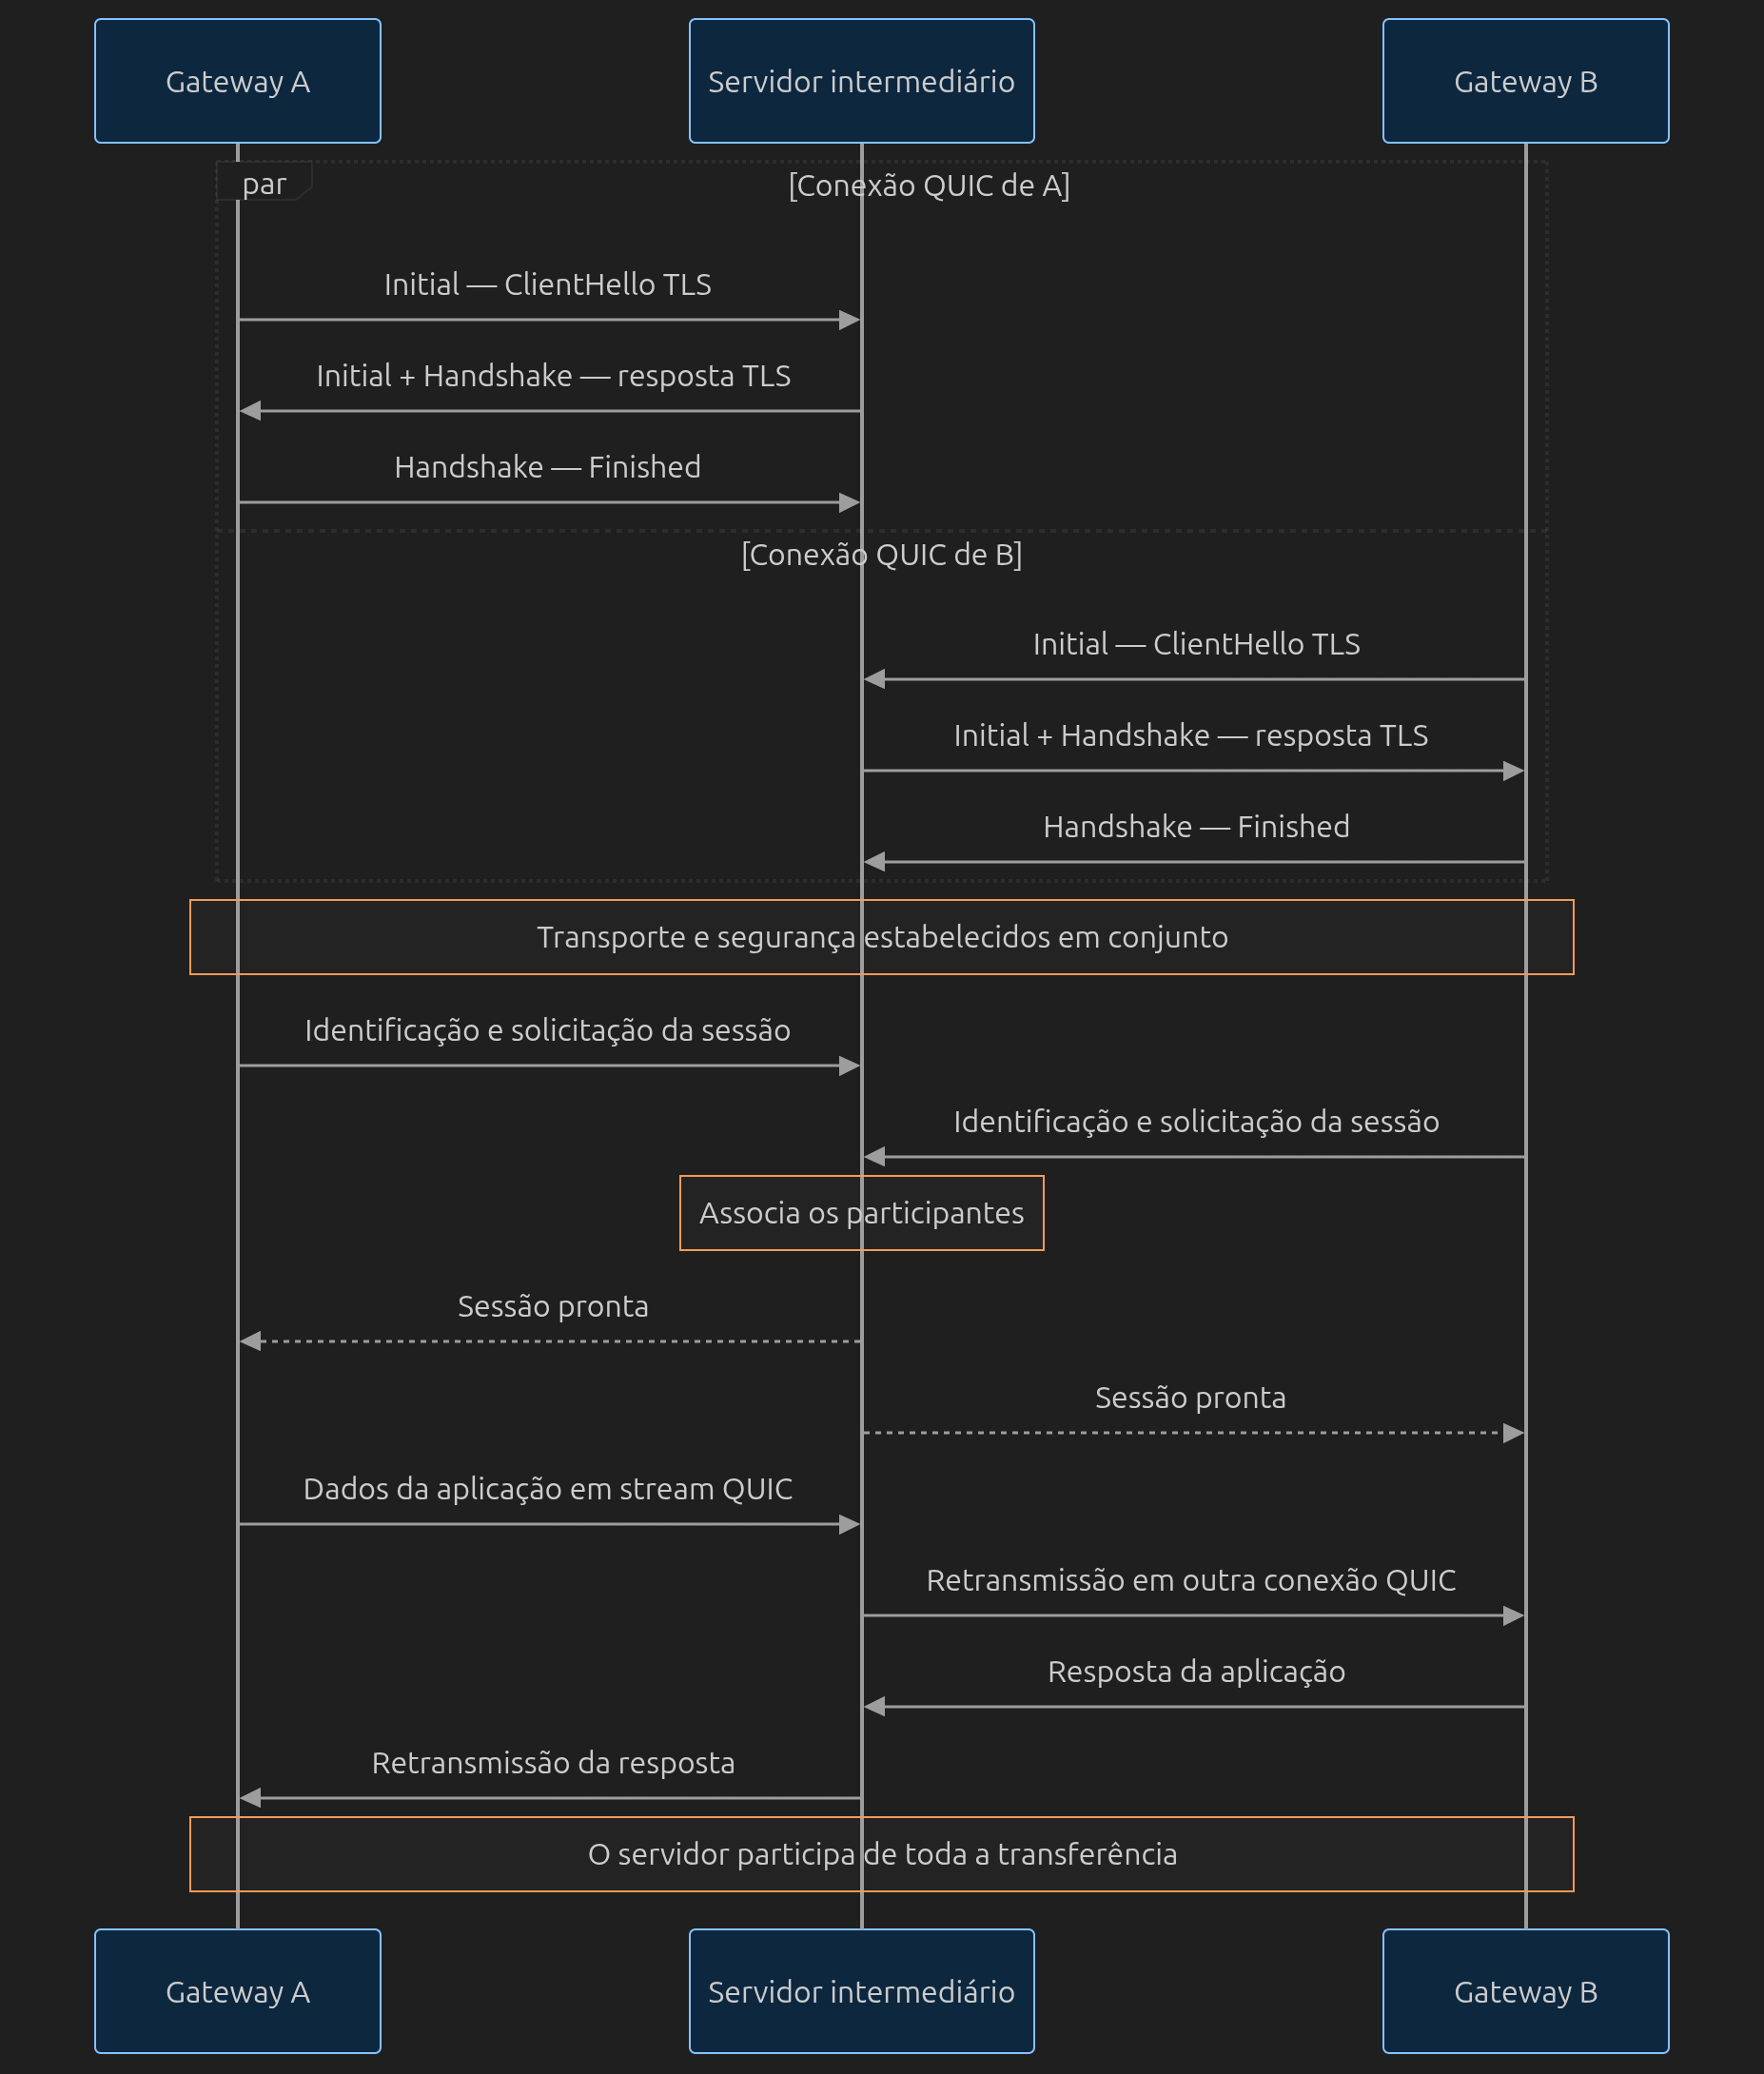
\includegraphics[width=0.8\textwidth]{fig/results/logic/centralized_server_quic_flow.png}
    \caption{Diagrama de tempo das etapas de comunicação utilizando um servidor especializado.}
    \label{fig:centralized_server_quic_flow}
\end{figure}

\subsection{Comunicação P2P com TCP hole punching}

Ao se utilizar TCP \textit{hole punching} sobre ICE, como descrito por \citep{rfc6544}, a comunicação entre os \textit{peers} ocorre de forma semelhante ao ICE para UDP descrito na Seção~\ref{sec:ice}. Entretanto, como o TCP não permite o envio de dados antes da existência de uma conexão estabelecida, é necessário realizar o TCP \textit{hole punching} de forma prévia à realização dos \textit{connectivity checks}; desta forma, os \textit{connectivity checks} mantêm como função principal a autenticação de cada par, e não mais a própria verificação de conectividade. Este fluxo pode ser visto na Figura~\ref{fig:non_centralized_ice_tcp_flow}.

\begin{figure}[!ht]
    \centering
    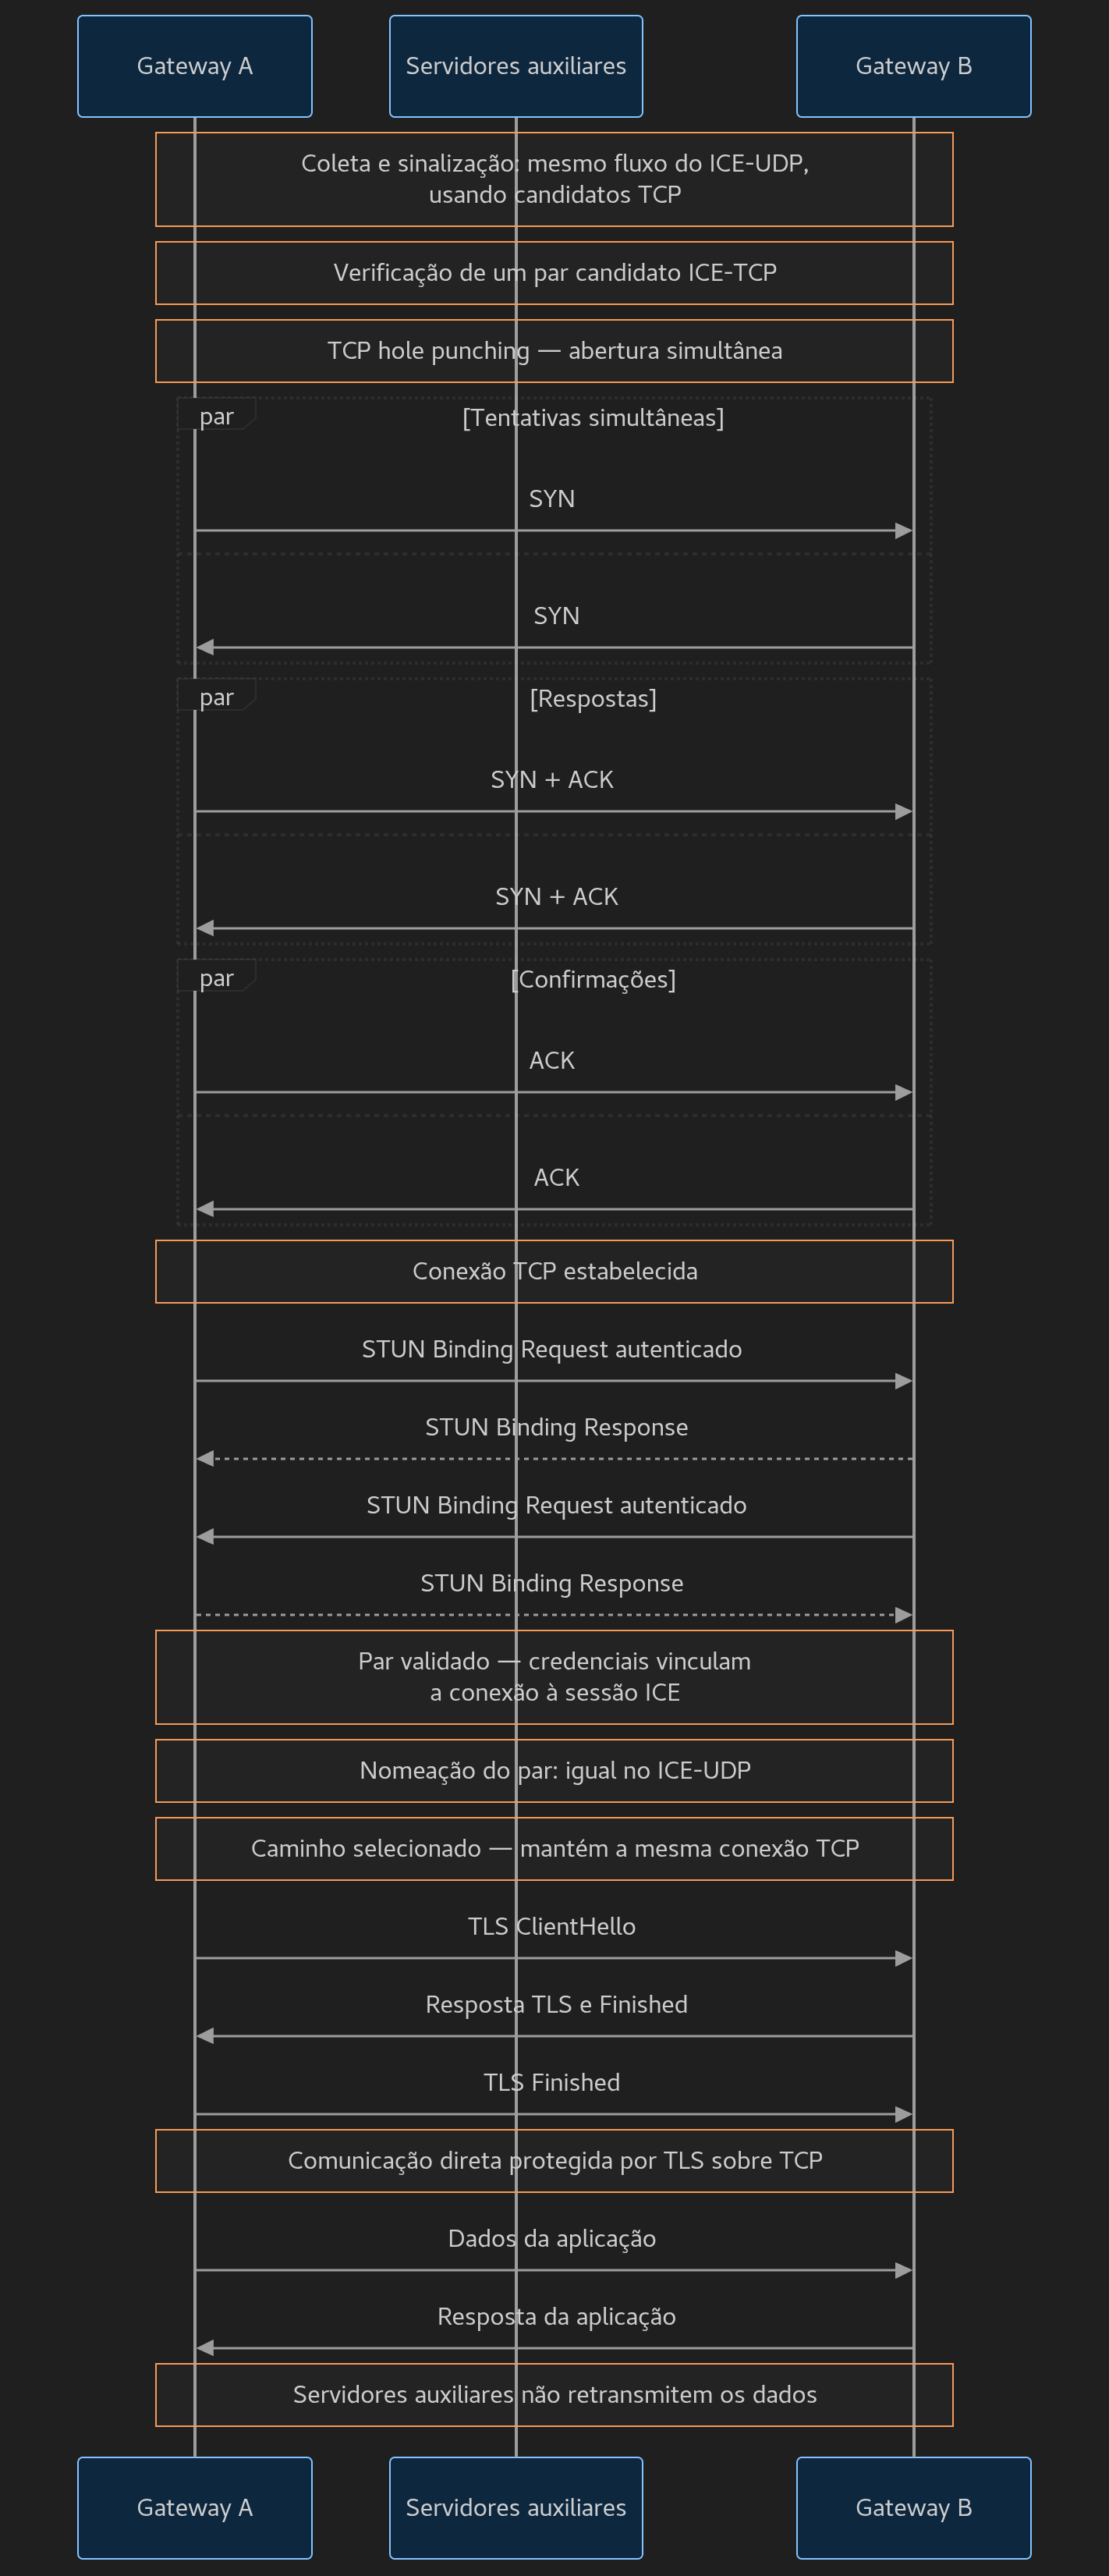
\includegraphics[width=0.5\textwidth]{fig/results/logic/flow_ice_tcp.png}
    \caption{Diagrama de tempo das etapas de comunicação utilizando ICE com TCP \textit{hole punching}.}
    \label{fig:non_centralized_ice_tcp_flow}
\end{figure}

\subsection{Comparação conceitual entre as abordagens}

Ao se utilizar uma conexão direta com o servidor, como proposto na Figura~\ref{fig:centralized_server_quic_flow}, o próprio servidor passa a ter acesso aos dados da aplicação, sem garantia de confidencialidade, dado que ele possui as chaves privadas tanto da conexão com o \textit{gateway}/\textit{peer} A quanto do \textit{gateway}/\textit{peer} B. Isto implica a necessidade de uma camada adicional de proteção dos dados de aplicação sobre essa comunicação, que não pode ser provida apenas pela camada de transporte. No caso do uso de um servidor TURN como \textit{fallback} da abordagem P2P, isto não ocorre: os dados enviados ao servidor são tunelados via TURN, e não por meio de uma conexão QUIC direta com o servidor, ou seja, a conexão QUIC permanece estabelecida de ponta a ponta entre os \textit{peers}, e o servidor TURN apenas retransmite os pacotes já cifrados.

Além disso, por se tratar de um servidor especializado, caso haja a queda deste, não há um servidor secundário que possa ser consultado para garantir a disponibilidade do serviço, o que não ocorre nas abordagens P2P, pois a solução é genérica e depende apenas de outro servidor que implemente o protocolo (não dependendo, por exemplo, de acesso direto a um banco de dados ou de alguma gerência específica).

Como visto por \citep{ford2005peer}, grande parte dos dispositivos NAT aceita técnicas de \textit{hole punching}, o que reduz a ocorrência da necessidade de uso de um servidor \textit{relay}/TURN nas abordagens P2P, tornando o cenário de indireção descrito como desvantagem da abordagem centralizada menos frequente na prática do que poderia parecer à primeira vista.

Ao utilizar técnicas de TCP \textit{hole punching}, é possível notar pela Figura~\ref{fig:non_centralized_ice_tcp_flow} que o estabelecimento da comunicação fica ainda mais lento: além da validação de candidatos, ainda é necessária a realização de uma dupla conexão TCP simultânea, adicionando mais dois \textit{3-way handshakes}. Além disso, a criptografia depende do TLS, que roda de forma separada do TCP, adicionando ainda outro \textit{handshake}.

Do ponto de vista operacional, as conexões TCP também podem ser consideradas mais frágeis por manterem metadados da conexão, como o número de sequência, expostos em texto claro, ao contrário do QUIC, que, como visto na Seção~\ref{sec:quic_header_protection}, protege criptograficamente essas informações mesmo no cabeçalho dos pacotes. Além disso, como visto por \citep{ford2005peer}, o TCP hole punching tem aproximadamente 20\% menos chance de efetivamente estabelecer a conexão do que o próprio UDP hole punching, além de possuir grandes dependências de sincronização, descritas na Seção~\ref{sec:tcp_hole_punching}.

\chapter{Conclusão}
\label{chap:conclusion}

%\bibliographystyle{ppgcc-alpha}
%\bibliographystyle{ppgcc-num}
\bibliographystyle{apalike}
\bibliography{ref.bib}

\appendix
%\include{src/atch_authProtocol}
%\include{src/atch_packetHandlerFSM}
%\include{src/atch_sbcci22}
%\include{src/atch_iscas23}

\anexos

%\includepdf[pages=-, pagecommand=\thispagestyle{headings}, addtotoc={1,chapter,Attachment A, pdf-sbcci}]{papers/sbcci22.pdf}





\end{document}
